\documentclass[aspectratio=169,12pt]{beamer}
\usepackage[utf8]{inputenc}
\usepackage[T5]{fontenc}
\usepackage[vietnamese]{babel}
\usepackage{lmodern}
\usepackage{graphicx}
\usepackage{booktabs}
\usepackage{tabularx}
\usepackage{multicol}
\usepackage{tikz}
\usepackage{xcolor}

\usetheme{Madrid}
\usefonttheme{professionalfonts}

% --- Custom Colors & Settings ---
\definecolor{UBrandBlue}{RGB}{0, 71, 155}
\definecolor{UBrandGold}{RGB}{255, 184, 28}
\setbeamercolor{palette primary}{bg=UBrandBlue,fg=white}
\setbeamercolor{palette secondary}{bg=UBrandGold,fg=black}
\setbeamercolor{palette tertiary}{bg=UBrandBlue!80!black,fg=white}
\setbeamercolor{title}{bg=UBrandBlue,fg=white}
\setbeamercolor{item}{fg=UBrandBlue}


\title[Thực hành - Chương 03]{Động lực và Mục tiêu Phân tích Dữ liệu}
\subtitle{Motivations and Objectives for Data Analysis}
\author[Giảng viên]{Trí tuệ Nhân tạo cho Kế toán (AI in Accounting)}
\institute[Đại học]{Khoa Kế toán - Kiểm toán}
\date{Bài giảng Thực hành 03}

\begin{document}

\begin{frame}
    \titlepage
\end{frame}

\begin{frame}{Góc nhìn Chuyên gia (Professional Insight)}
\begin{itemize}
    \item \textbf{Tầm quan trọng của Động lực và Mục tiêu:} Trong bất kỳ dự án phân tích dữ liệu nào, việc xác định rõ động lực và mục tiêu là bước khởi đầu mang tính quyết định.
    \item \textbf{Định hướng phân tích:} Giống như một chiếc la bàn, mục tiêu giúp kế toán viên không bị lạc lối giữa 'rừng' dữ liệu khổng lồ và phức tạp.
    \item \textbf{Tạo ra giá trị thực sự:} Nếu không có mục tiêu kinh doanh rõ ràng, các mô hình dữ liệu phức tạp nhất cũng trở nên vô nghĩa.
    \item \textbf{Sự phù hợp (Alignment):} Đảm bảo kết quả phân tích gắn liền với chiến lược của ban lãnh đạo và yêu cầu của các bên liên quan.
\end{itemize}
\end{frame}

\begin{frame}{Lộ trình Chương (Chapter Roadmap)}
\begin{itemize}
    \item \textbf{LO 3.1:} Mối quan hệ giữa Động lực, Mục tiêu và Câu hỏi Phân tích.
    \item \textbf{LO 3.2:} Phát triển Câu hỏi Mô tả (Điều gì đã xảy ra?).
    \item \textbf{LO 3.3:} Phát triển Câu hỏi Chẩn đoán (Tại sao lại xảy ra?).
    \item \textbf{LO 3.4:} Phát triển Câu hỏi Dự đoán (Điều gì sẽ xảy ra?).
    \item \textbf{LO 3.5:} Phát triển Câu hỏi Đề xuất (Chúng ta nên làm gì?).
    \item \textbf{LO 3.6:} Động lực và Mục tiêu trong Thực tiễn Nghề nghiệp Kế toán.
\end{itemize}
\end{frame}

\begin{frame}{3.1 Động lực định hình câu hỏi phân tích như thế nào?}
\begin{itemize}
    \item \textbf{Động lực (Motivation):} Là lý do sâu xa khởi tạo dự án phân tích dữ liệu. Nó phản ánh một nhu cầu chưa được đáp ứng hoặc một khoảng trống trong quy trình hiện tại.
    \item \textbf{Tác động đến quy trình:} Động lực sẽ quyết định cách chúng ta tiếp cận dữ liệu, lựa chọn công cụ và xác định mức độ chi tiết của phân tích.
    \item \textbf{Cơ sở cho Câu hỏi Phân tích:} Một động lực mạnh mẽ sẽ trực tiếp dẫn dắt đến việc đặt ra các câu hỏi phân tích sắc bén và đi đúng vào trọng tâm của vấn đề nghiệp vụ.
\end{itemize}
\end{frame}

\begin{frame}{Mục tiêu Rõ ràng (Clear Objectives)}
\begin{itemize}
    \item \textbf{Chuyển hóa Động lực thành Mục tiêu:} Từ một động lực chung chung (VD: "Cải thiện doanh số"), chúng ta cần một mục tiêu cụ thể (VD: "Phân tích doanh số theo từng khu vực để tìm ra vùng có hiệu suất kém nhất").
    \item \textbf{Tính tập trung:} Mục tiêu rõ ràng loại bỏ các phân tích dư thừa không cần thiết (Noise) và tiết kiệm tài nguyên.
    \item \textbf{Xây dựng bộ chỉ số đo lường:} Mục tiêu giúp định nghĩa các KPI (Key Performance Indicators) để đánh giá mức độ thành công của dự án.
\end{itemize}
\end{frame}

\begin{frame}{Xác định Mục tiêu (Determine the Objective)}
\begin{itemize}
    \item \textbf{Quy tắc SMART:} Mục tiêu phân tích cần đạt được các tiêu chí: Cụ thể (Specific), Đo lường được (Measurable), Có thể đạt được (Achievable), Thực tế (Realistic) và Có thời hạn (Time-bound).
    \item \textbf{Tính lặp lại (Iterative):} Mục tiêu có thể thay đổi và tinh chỉnh khi dữ liệu bắt đầu được khám phá và bộc lộ những góc nhìn mới.
    \item \textbf{Sự tham gia của các bên liên quan:} Đảm bảo sự đồng thuận giữa kế toán viên, nhà phân tích và nhà quản trị đối với mục tiêu được đề ra.
\end{itemize}
\end{frame}

\begin{frame}{Kết nối Động lực với Mục tiêu}
\begin{itemize}
    \item \textbf{Ví dụ trong Kiểm toán:}
    \item \textbf{Động lực:} Rủi ro sai sót trọng yếu đối với các khoản phải thu thương mại tăng cao trong bối cảnh suy thoái kinh tế.
    \item \textbf{Mục tiêu:} Phân tích tuổi nợ của toàn bộ danh mục khách hàng để trích lập dự phòng phải thu khó đòi chính xác.
    \item \textbf{Câu hỏi Phân tích:} "Tỷ lệ nợ quá hạn trên 90 ngày của các khách hàng tại khu vực A là bao nhiêu?".
\end{itemize}
\end{frame}

\begin{frame}{ILLUSTRATION 3.1}

    \begin{figure}[h]
        \centering
        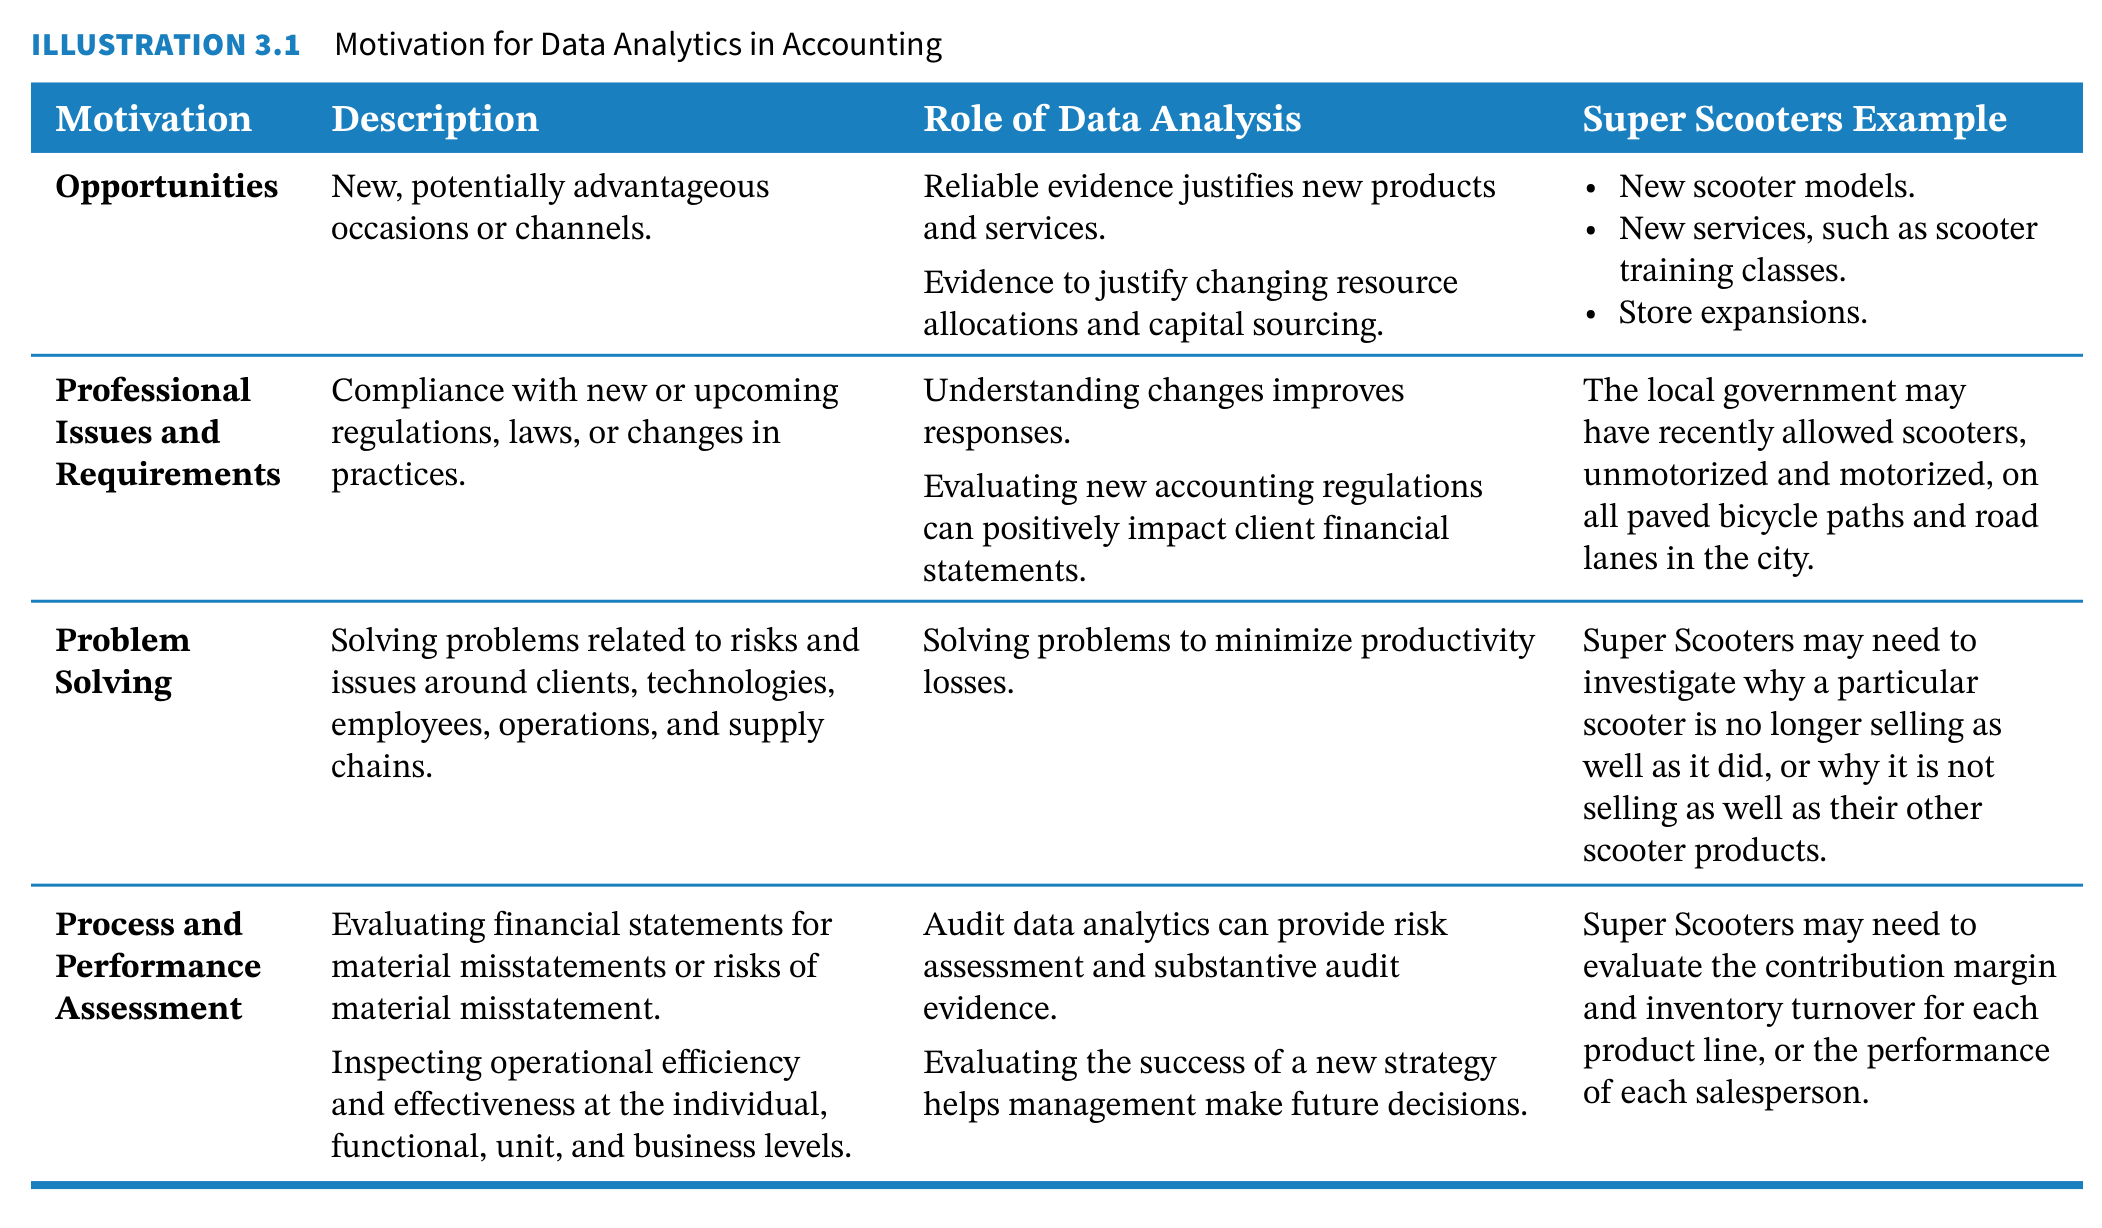
\includegraphics[width=0.95\textwidth,height=0.75\textheight,keepaspectratio]{../textbookForPractice/Figures/Ch_03/ILLUSTRATION 3.1.png}
    \end{figure}
\end{frame}

\begin{frame}{ILLUSTRATION 3.2}

    \begin{figure}[h]
        \centering
        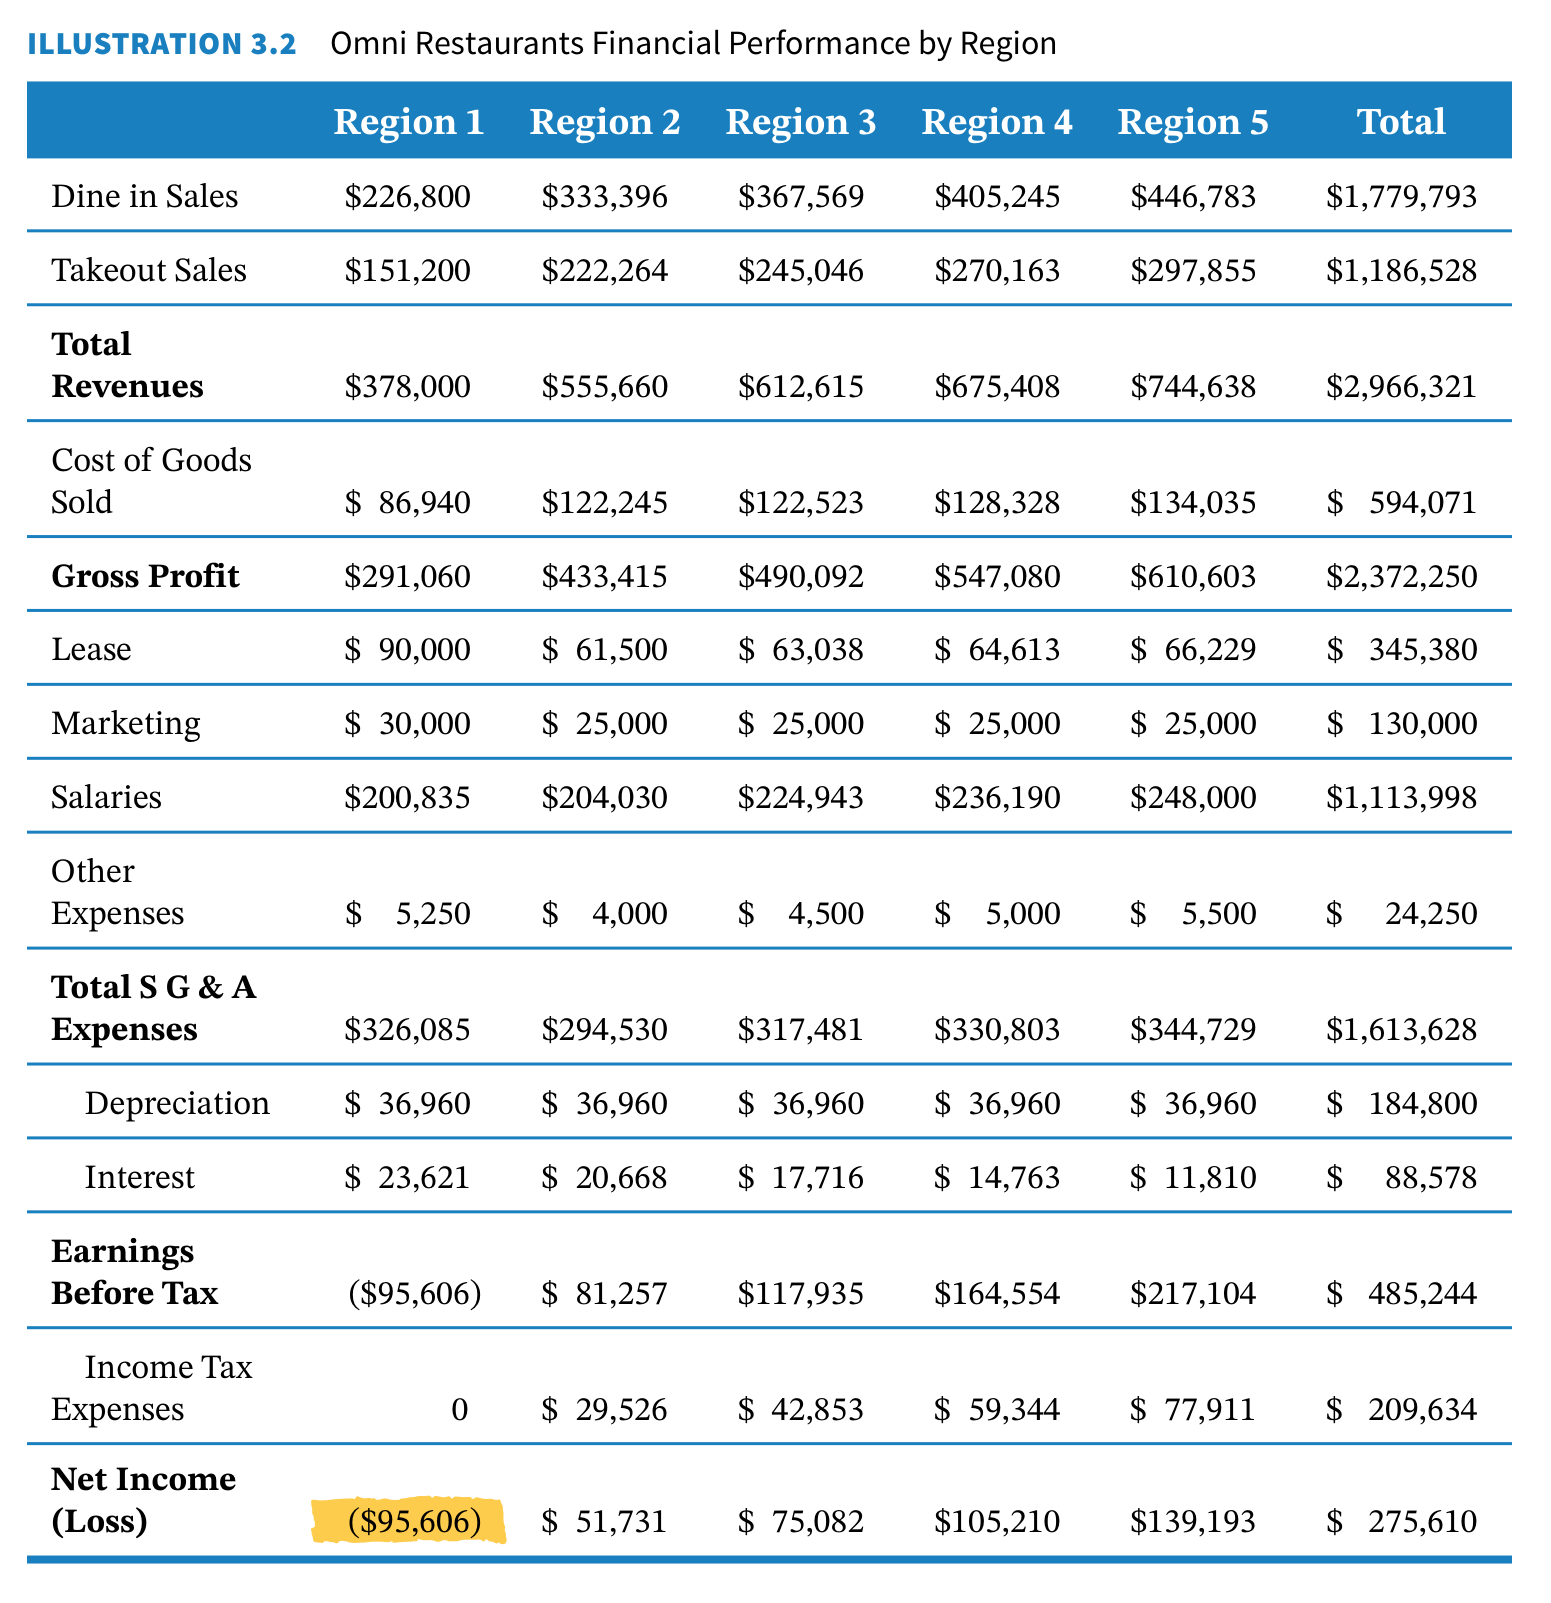
\includegraphics[width=0.95\textwidth,height=0.75\textheight,keepaspectratio]{../textbookForPractice/Figures/Ch_03/ILLUSTRATION 3.2.png}
    \end{figure}
\end{frame}

\begin{frame}{ILLUSTRATION 3.3}

    \begin{figure}[h]
        \centering
        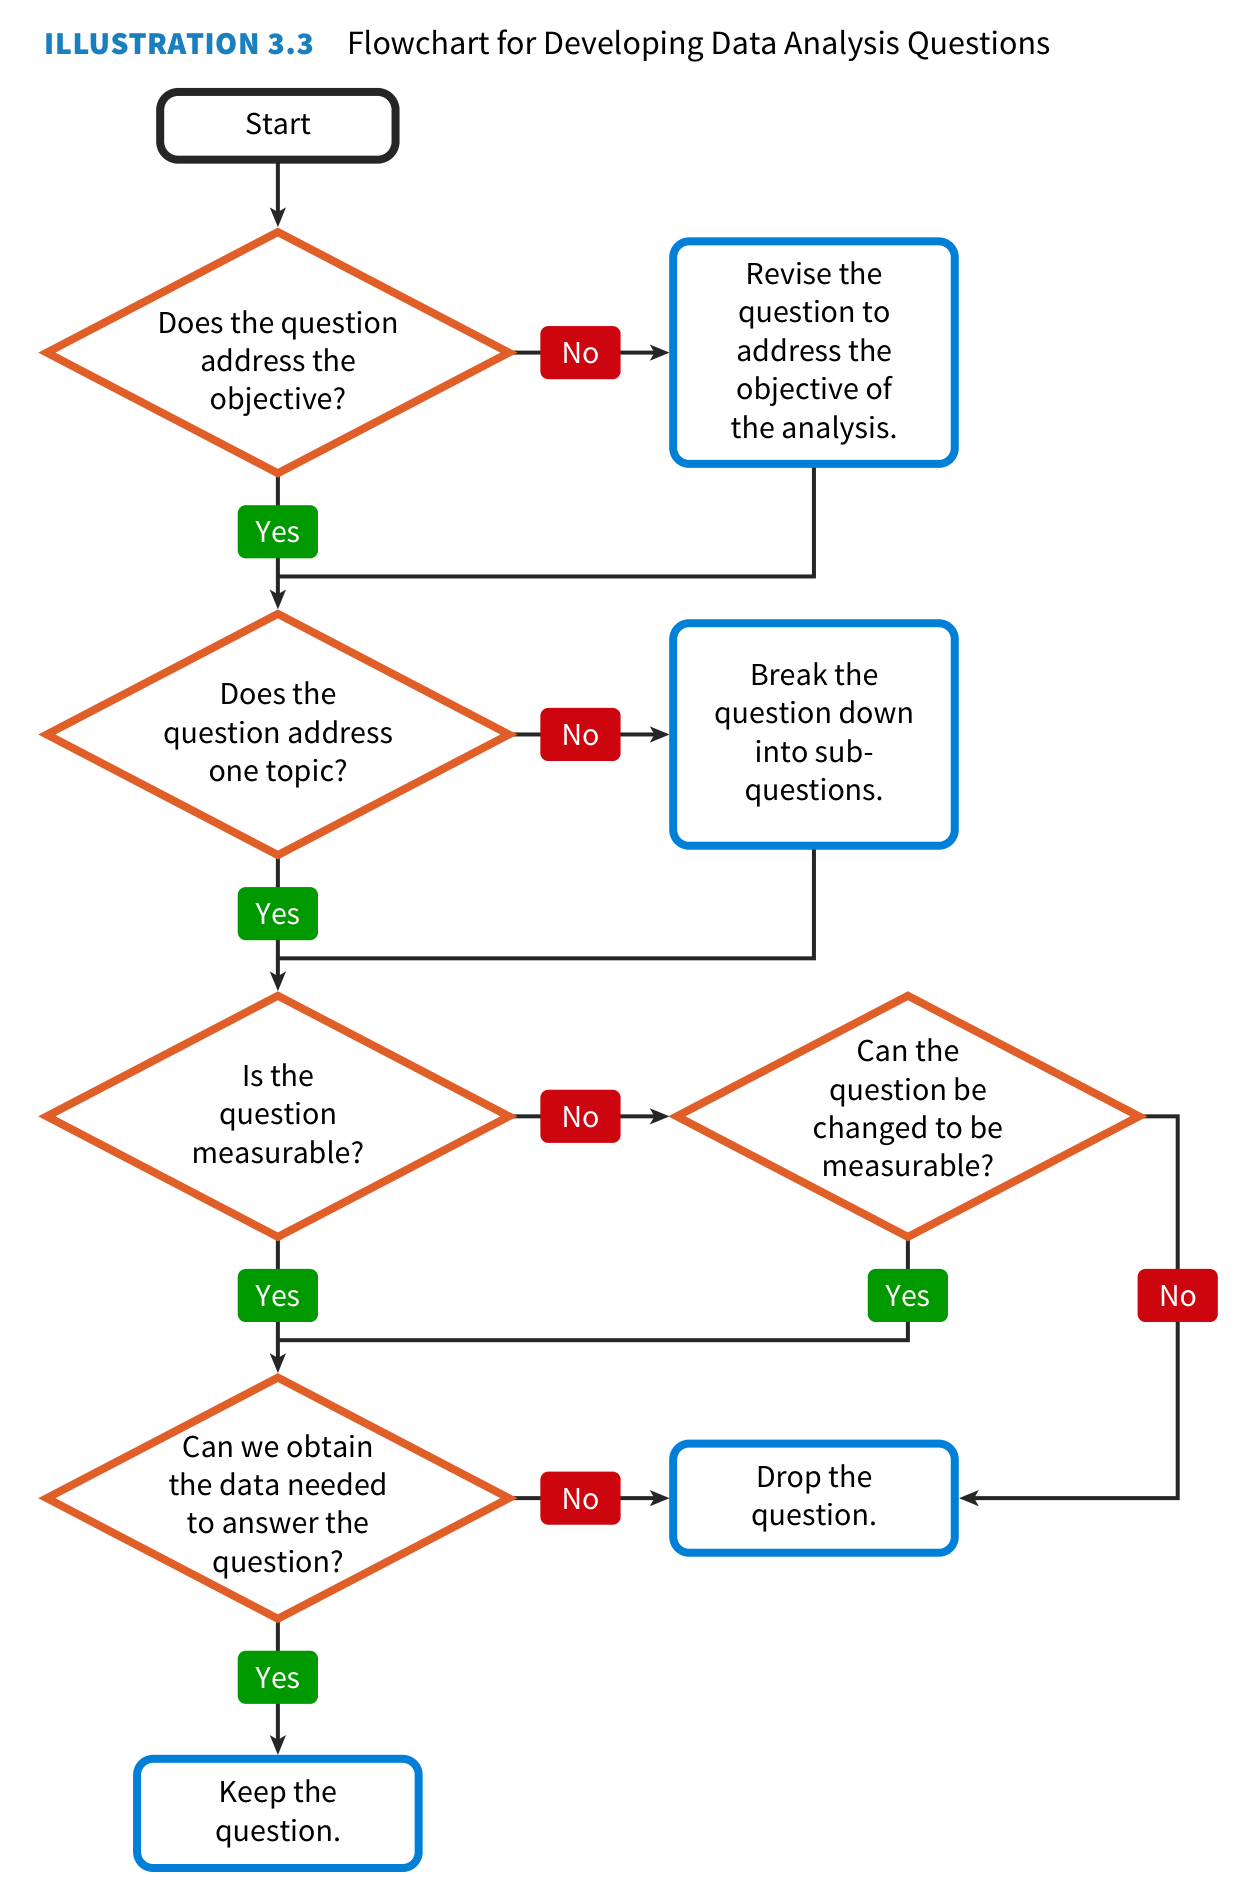
\includegraphics[width=0.95\textwidth,height=0.75\textheight,keepaspectratio]{../textbookForPractice/Figures/Ch_03/ILLUSTRATION 3.3.png}
    \end{figure}
\end{frame}

\begin{frame}{ILLUSTRATION 3.4}

    \begin{figure}[h]
        \centering
        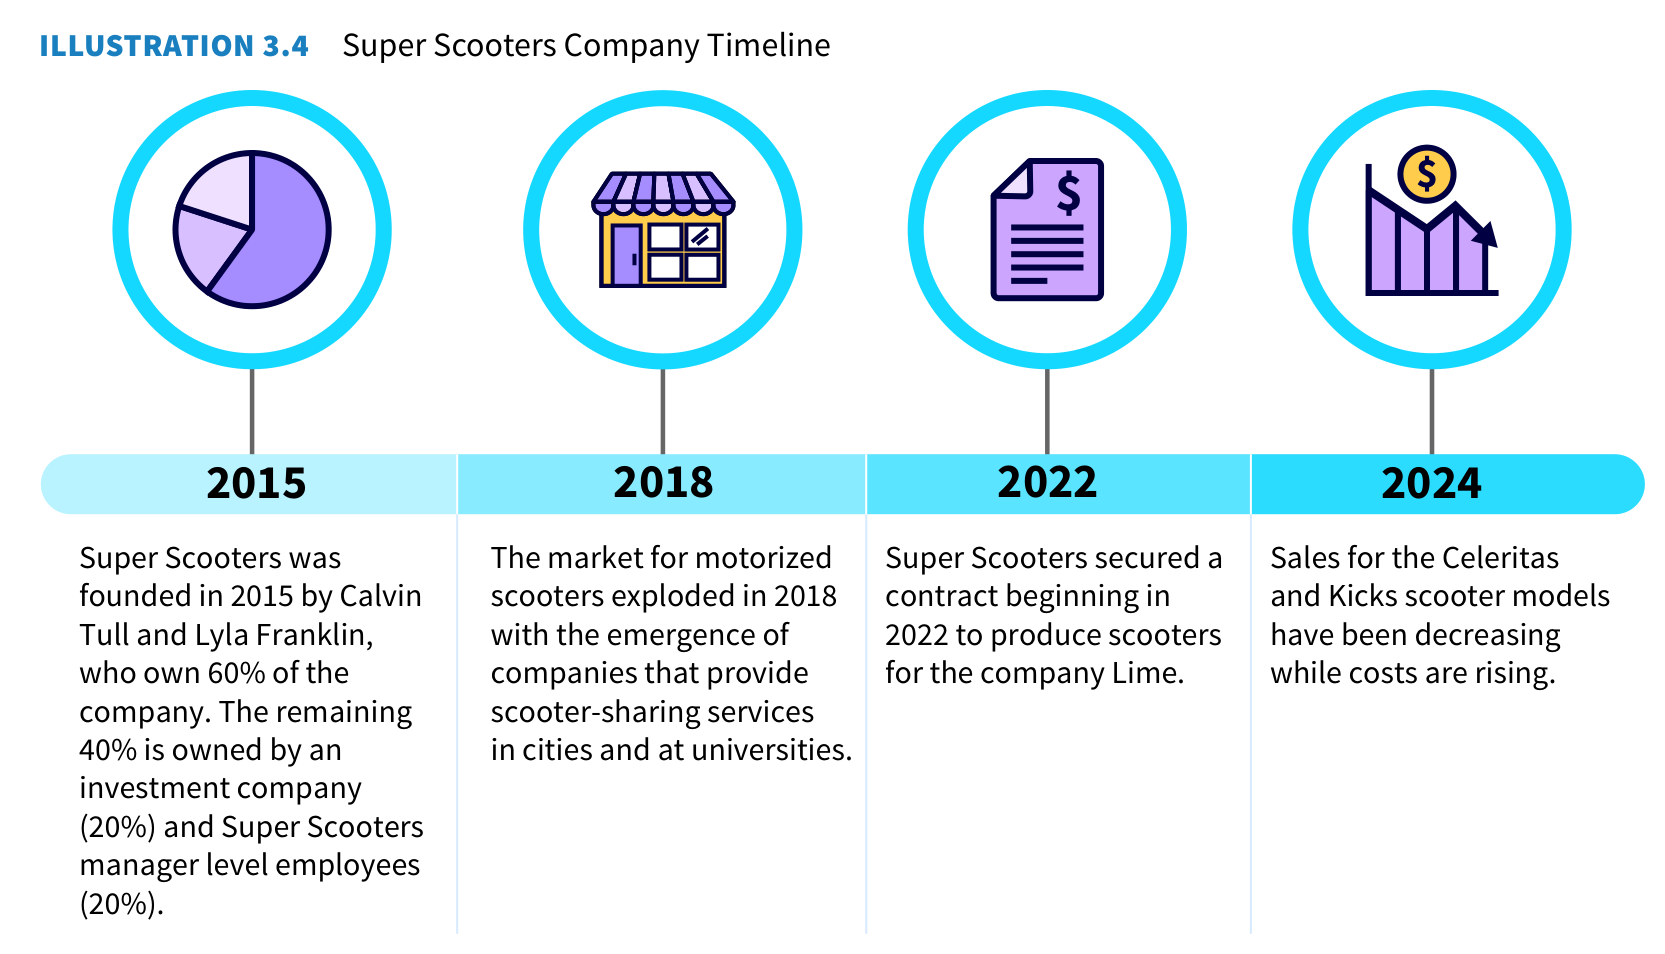
\includegraphics[width=0.95\textwidth,height=0.75\textheight,keepaspectratio]{../textbookForPractice/Figures/Ch_03/ILLUSTRATION 3.4.png}
    \end{figure}
\end{frame}

\begin{frame}{ILLUSTRATION 3.5}

    \begin{figure}[h]
        \centering
        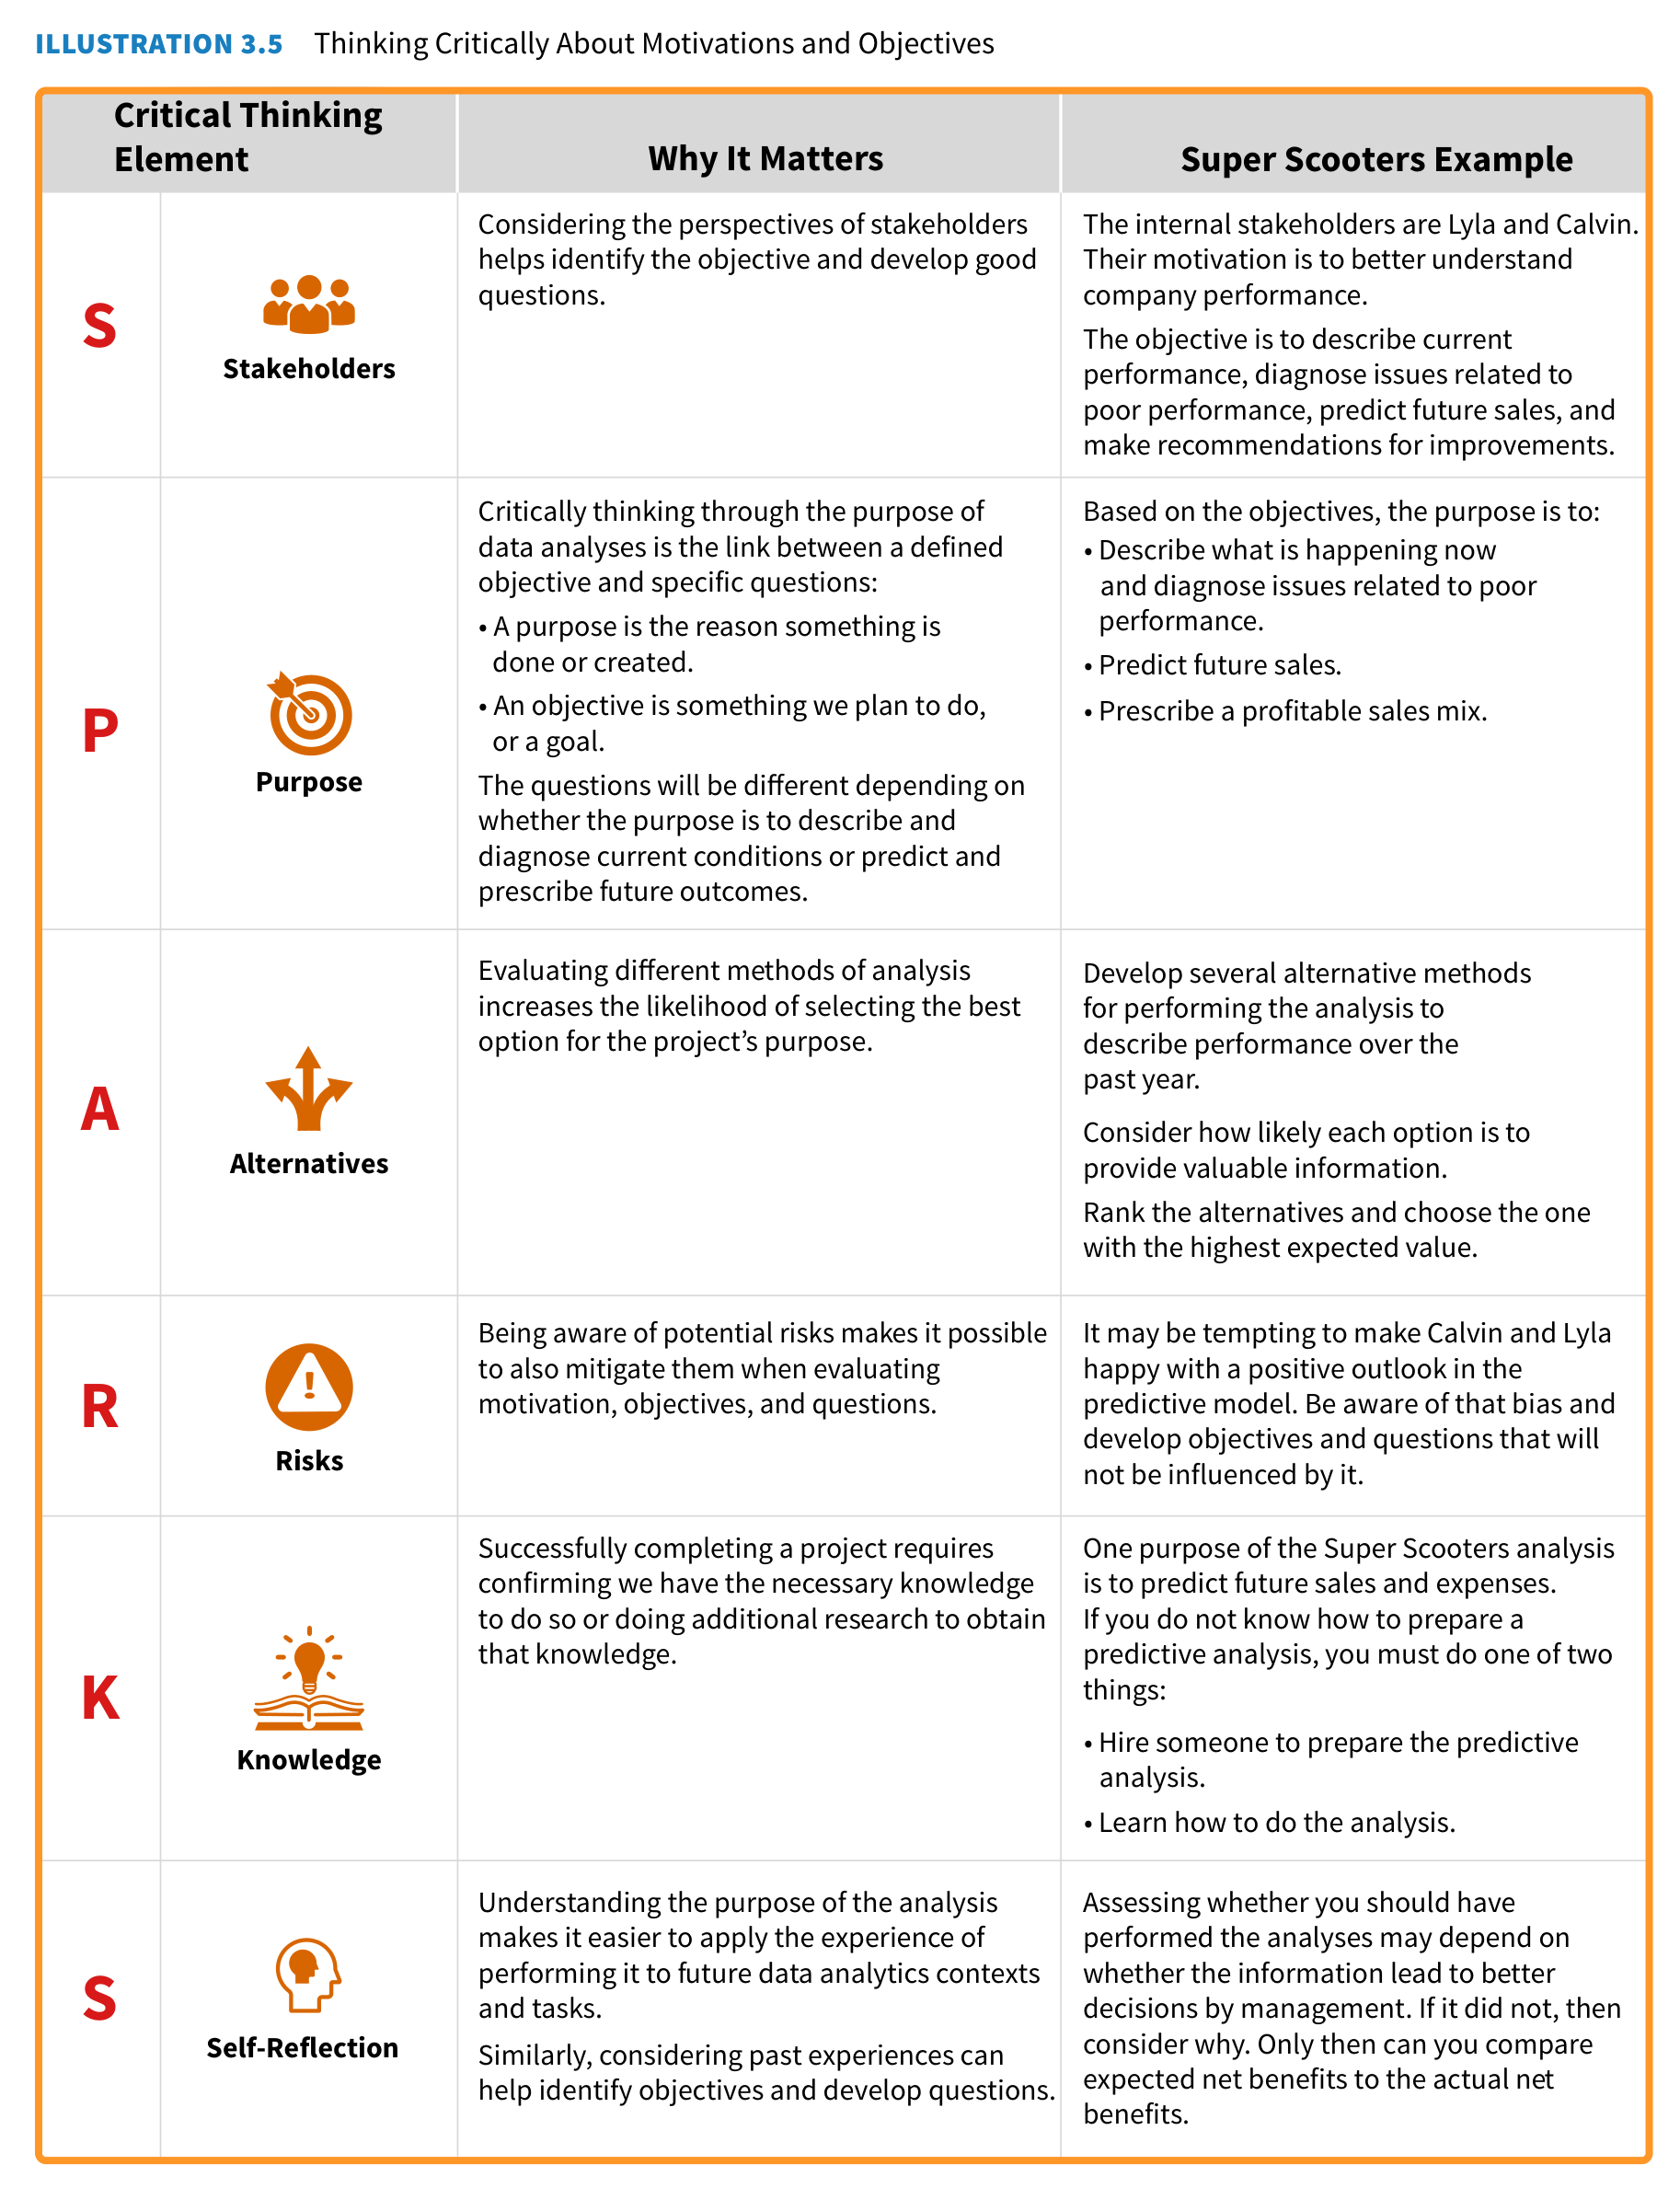
\includegraphics[width=0.95\textwidth,height=0.75\textheight,keepaspectratio]{../textbookForPractice/Figures/Ch_03/ILLUSTRATION 3.5.png}
    \end{figure}
\end{frame}

\begin{frame}{ILLUSTRATION 3.6}

    \begin{figure}[h]
        \centering
        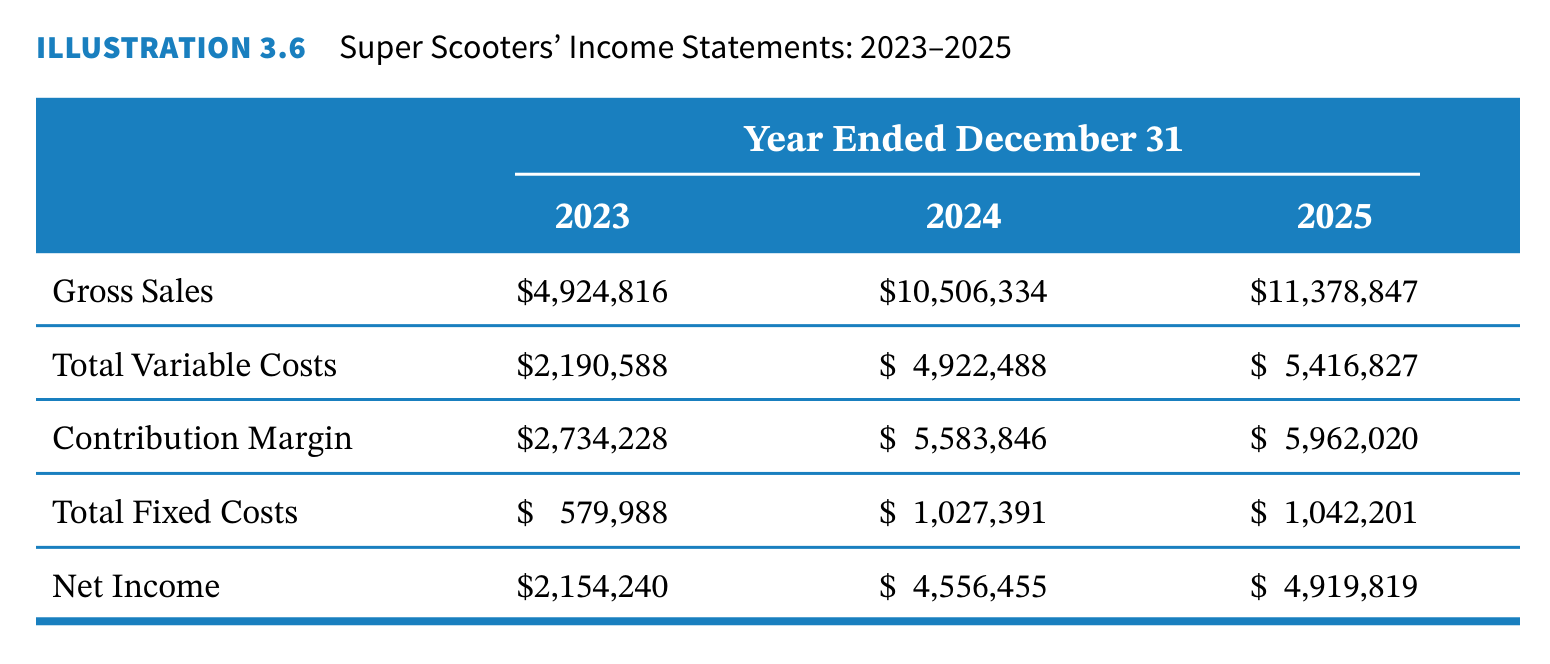
\includegraphics[width=0.95\textwidth,height=0.75\textheight,keepaspectratio]{../textbookForPractice/Figures/Ch_03/ILLUSTRATION 3.6.png}
    \end{figure}
\end{frame}

\begin{frame}{ILLUSTRATION 3.7}

    \begin{figure}[h]
        \centering
        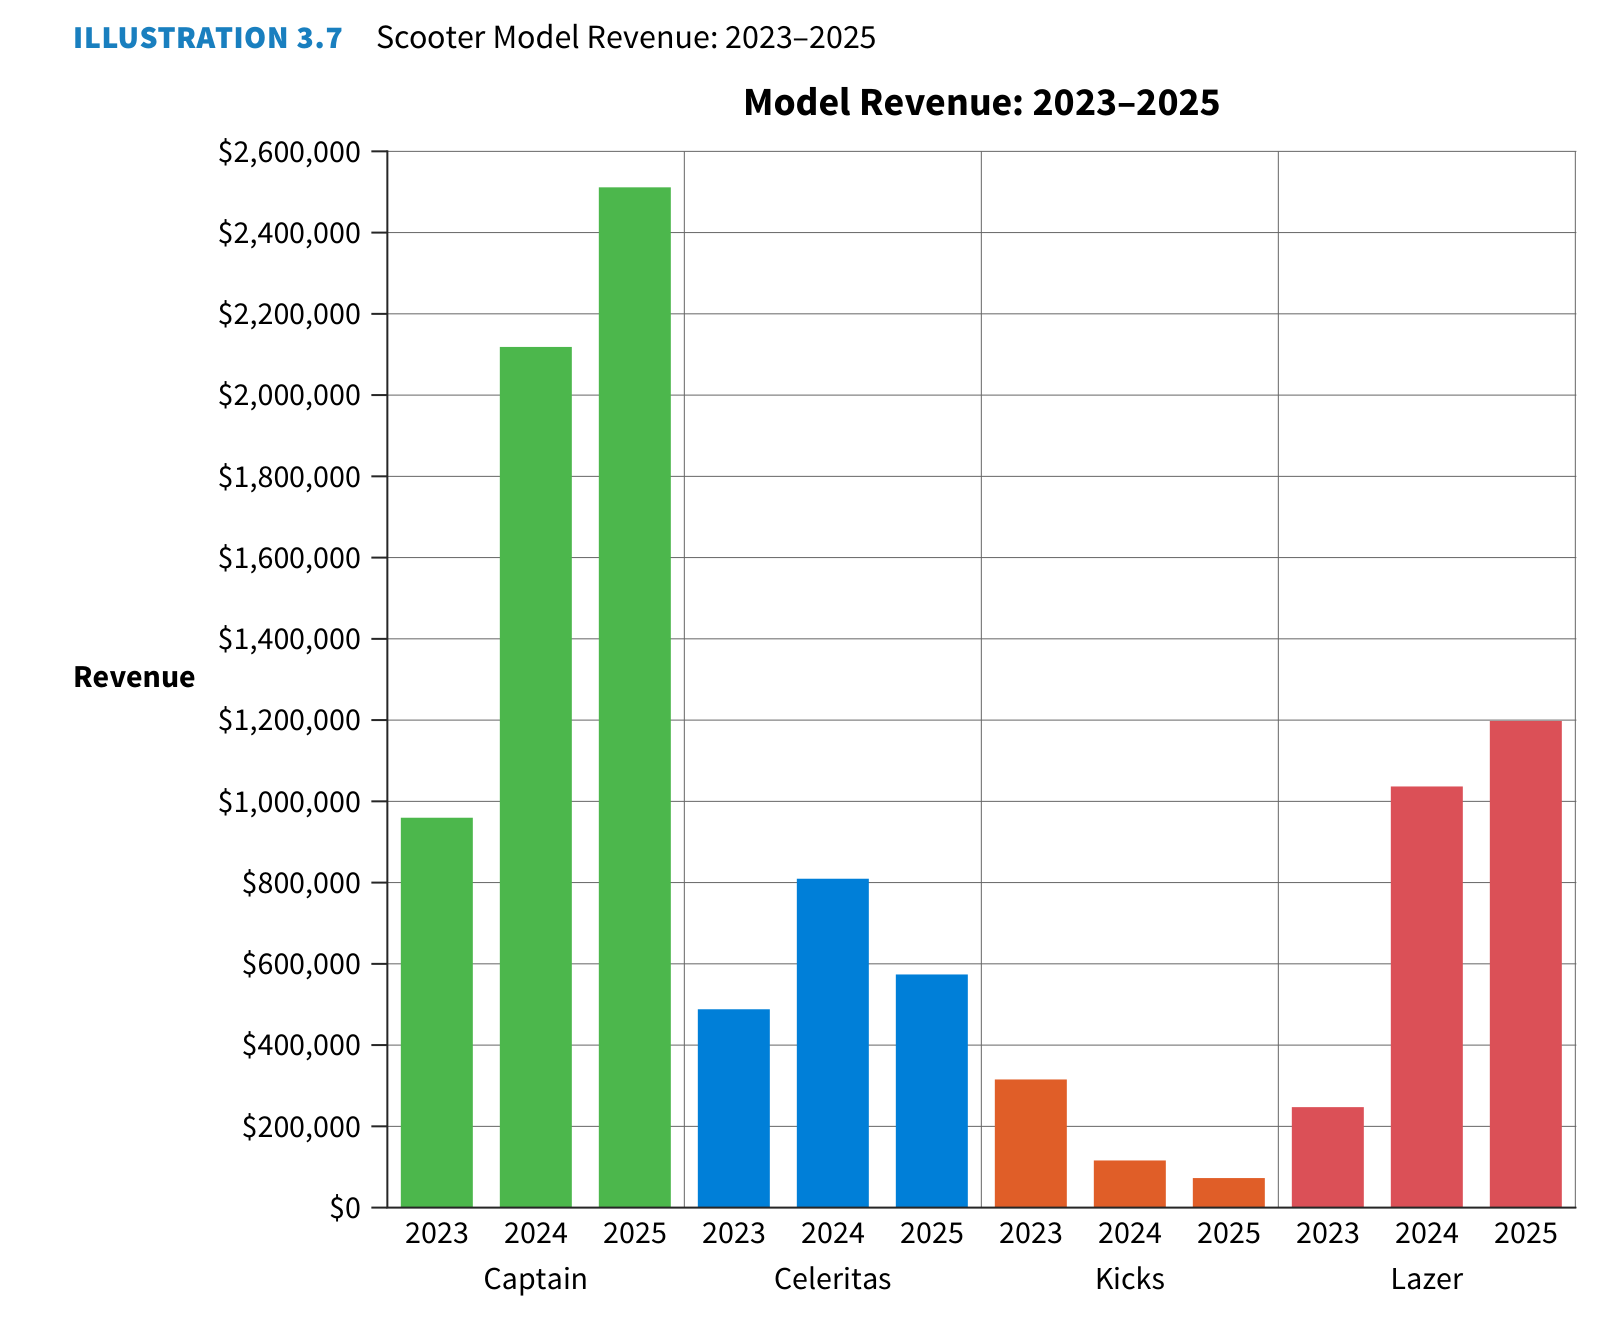
\includegraphics[width=0.95\textwidth,height=0.75\textheight,keepaspectratio]{../textbookForPractice/Figures/Ch_03/ILLUSTRATION 3.7.png}
    \end{figure}
\end{frame}

\begin{frame}{ILLUSTRATION 3.8}

    \begin{figure}[h]
        \centering
        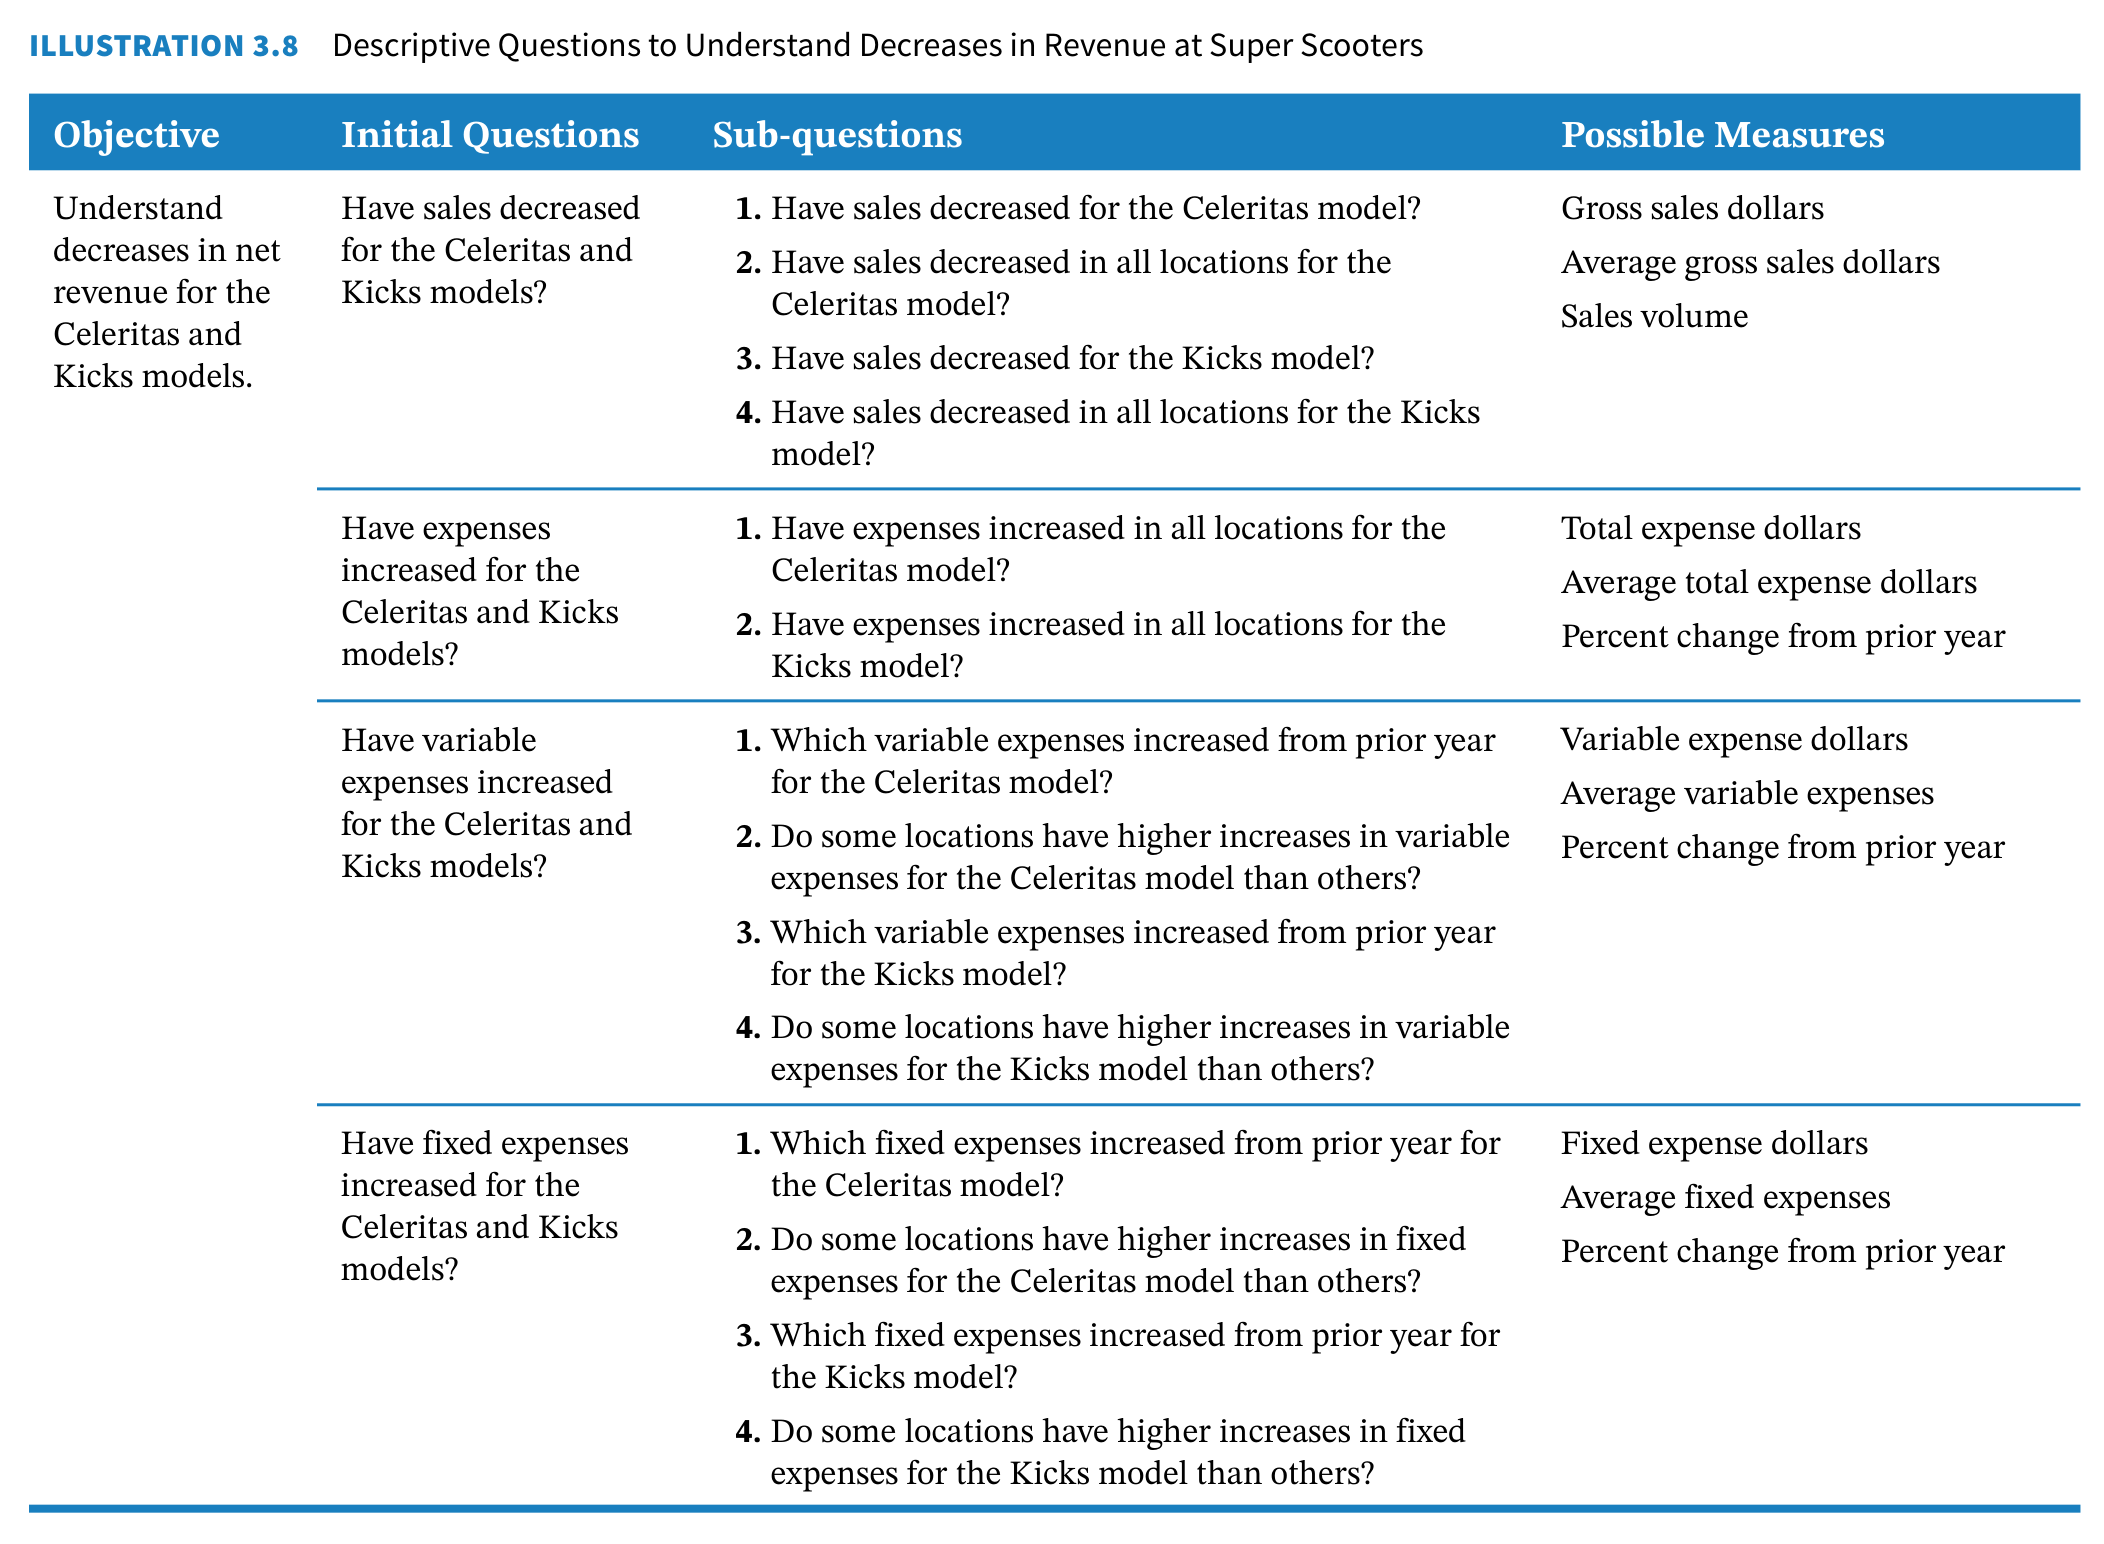
\includegraphics[width=0.95\textwidth,height=0.75\textheight,keepaspectratio]{../textbookForPractice/Figures/Ch_03/ILLUSTRATION 3.8.png}
    \end{figure}
\end{frame}

\begin{frame}{ILLUSTRATION 3.9}

    \begin{figure}[h]
        \centering
        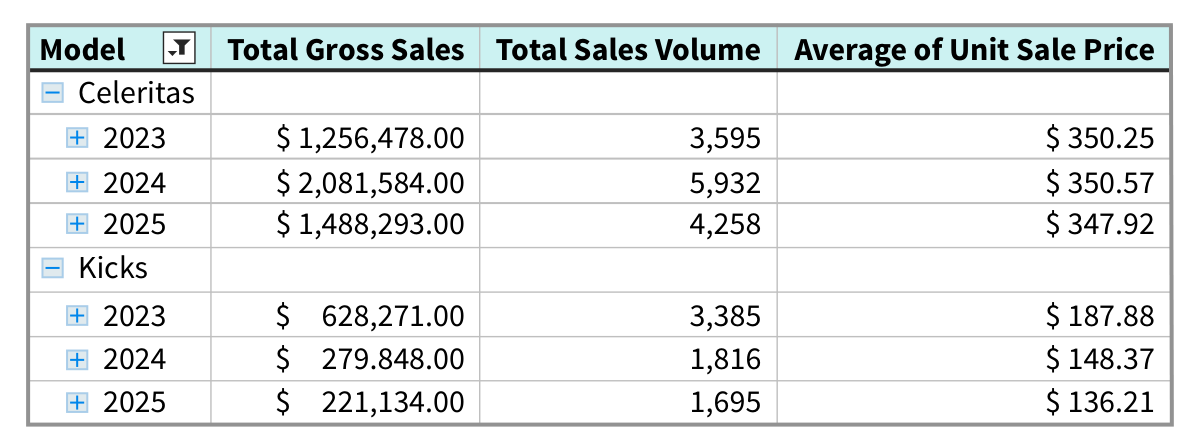
\includegraphics[width=0.95\textwidth,height=0.75\textheight,keepaspectratio]{../textbookForPractice/Figures/Ch_03/ILLUSTRATION 3.9.png}
    \end{figure}
\end{frame}

\begin{frame}{3.2 Làm thế nào để phát triển Câu hỏi Mô tả?}
\begin{itemize}
    \item \textbf{Câu hỏi Mô tả (Descriptive Questions):} Là nền tảng của mọi quá trình phân tích dữ liệu. Chúng tập trung vào việc tóm tắt thông tin đã diễn ra trong quá khứ.
    \item \textbf{Trọng tâm cốt lõi:} Tìm câu trả lời cho câu hỏi \textbf{"Điều gì đã xảy ra?"} (What happened?).
    \item \textbf{Vai trò:} Giúp tạo ra một bức tranh toàn cảnh về tình hình tài chính và hoạt động của doanh nghiệp trước khi đi sâu vào phân tích nguyên nhân hay dự đoán tương lai.
\end{itemize}
\end{frame}

\begin{frame}{Đặc điểm của Câu hỏi Mô tả}
\begin{itemize}
    \item \textbf{Bản chất:} Tập trung vào dữ liệu lịch sử (Historical data) như doanh số bán hàng, chi phí nhân công, hoặc dòng tiền trong quý trước.
    \item \textbf{Kết quả đầu ra:} Thường dưới dạng báo cáo định kỳ (Dashboards, Báo cáo tài chính) hoặc các bảng tóm tắt số liệu.
    \item \textbf{Công cụ phổ biến:} Các chỉ số thống kê mô tả (Mean, Median, Mode, Variance) và các biểu đồ cơ bản (Bar chart, Line chart).
\end{itemize}
\end{frame}

\begin{frame}{Phân loại Câu hỏi Mô tả trong Kế toán}
\begin{itemize}
    \item \textbf{Theo dõi biến động:} Doanh thu tháng này thay đổi như thế nào so với cùng kỳ năm trước?
    \item \textbf{Phân loại và Nhóm:} Số lượng giao dịch vượt quá định mức phê duyệt là bao nhiêu?
    \item \textbf{Tóm tắt sự kiện:} Đâu là 5 khách hàng mang lại tỷ suất lợi nhuận lớn nhất trong năm?
    \item \textbf{Chỉ số hiệu suất:} Chi phí sản xuất trung bình trên một đơn vị sản phẩm là bao nhiêu?
\end{itemize}
\end{frame}

\begin{frame}{Ví dụ Phân tích Mô tả (Kế toán Tài chính)}
\begin{itemize}
    \item \textbf{Bối cảnh:} Một doanh nghiệp bán lẻ muốn hiểu rõ hơn về hành vi mua hàng của khách hàng trong dịp lễ hội.
    \item \textbf{Câu hỏi Mô tả:} Tổng giá trị đơn hàng trung bình trong tháng 12 là bao nhiêu? Tỷ lệ trả hàng sau dịp lễ là bao nhiêu \%?
    \item \textbf{Hành động Kế toán:} Trích xuất dữ liệu từ hệ thống ERP, loại bỏ dữ liệu nhiễu và sử dụng Pivot Table để tổng hợp doanh thu theo từng ngành hàng.
\end{itemize}
\end{frame}

\begin{frame}{Dữ liệu bán hàng \& Trực quan hóa}
\begin{itemize}
    \item \textbf{Trực quan hóa Dữ liệu (Data Visualization):} Chuyển đổi các bảng số liệu khô khan thành biểu đồ trực quan, giúp nhà quản lý nắm bắt thông tin ngay lập tức.
    \item \textbf{Biểu đồ đường (Line Chart):} Hiển thị xu hướng doanh thu theo thời gian.
    \item \textbf{Biểu đồ cột (Bar Chart):} So sánh doanh thu giữa các khu vực địa lý hoặc cửa hàng.
    \item \textbf{Biểu đồ tròn (Pie Chart):} Thể hiện tỷ trọng của từng nhóm sản phẩm trong tổng doanh thu.
\end{itemize}
\end{frame}

\begin{frame}{ILLUSTRATION 3.10}

    \begin{figure}[h]
        \centering
        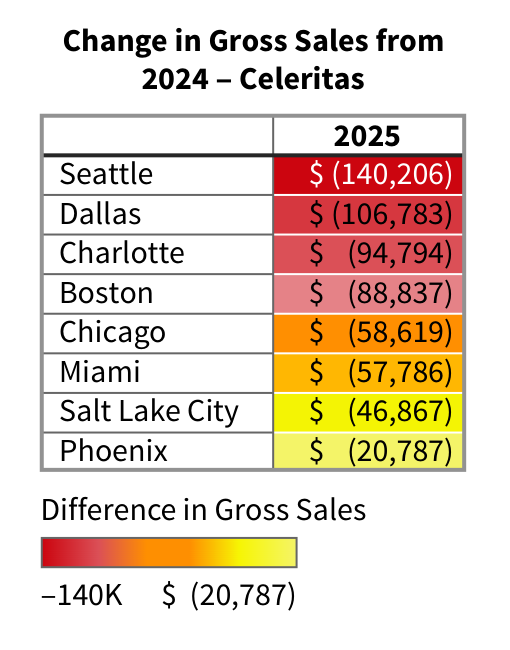
\includegraphics[width=0.95\textwidth,height=0.75\textheight,keepaspectratio]{../textbookForPractice/Figures/Ch_03/ILLUSTRATION 3.10.png}
    \end{figure}
\end{frame}

\begin{frame}{ILLUSTRATION 3.11}

    \begin{figure}[h]
        \centering
        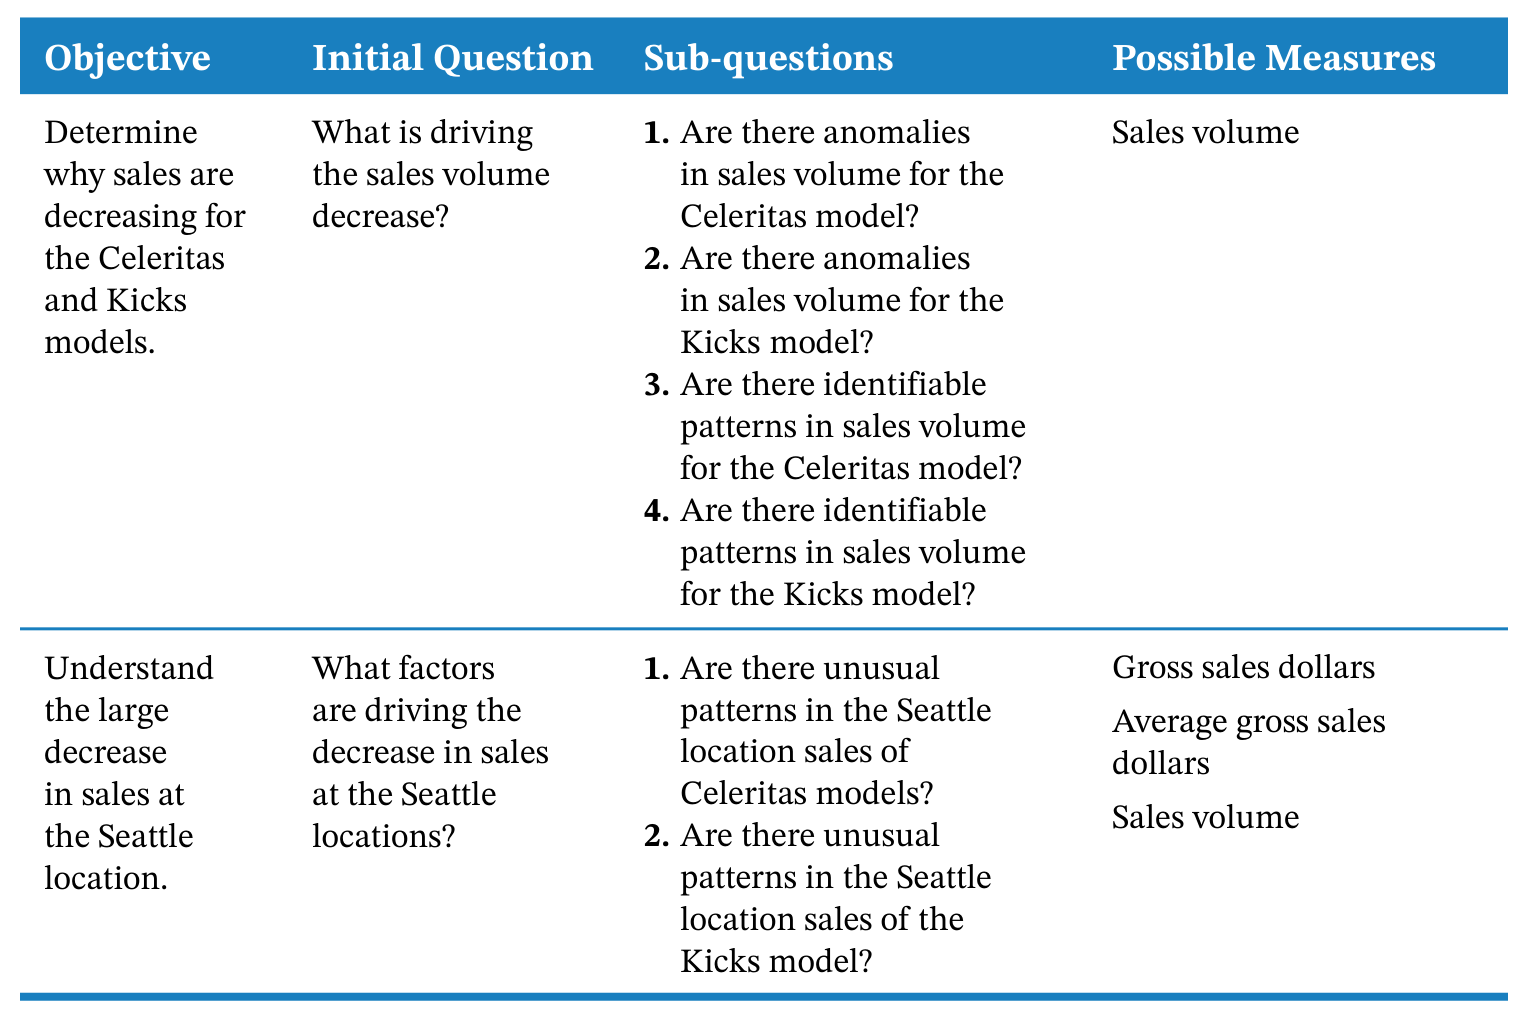
\includegraphics[width=0.95\textwidth,height=0.75\textheight,keepaspectratio]{../textbookForPractice/Figures/Ch_03/ILLUSTRATION 3.11.png}
    \end{figure}
\end{frame}

\begin{frame}{ILLUSTRATION 3.12}

    \begin{figure}[h]
        \centering
        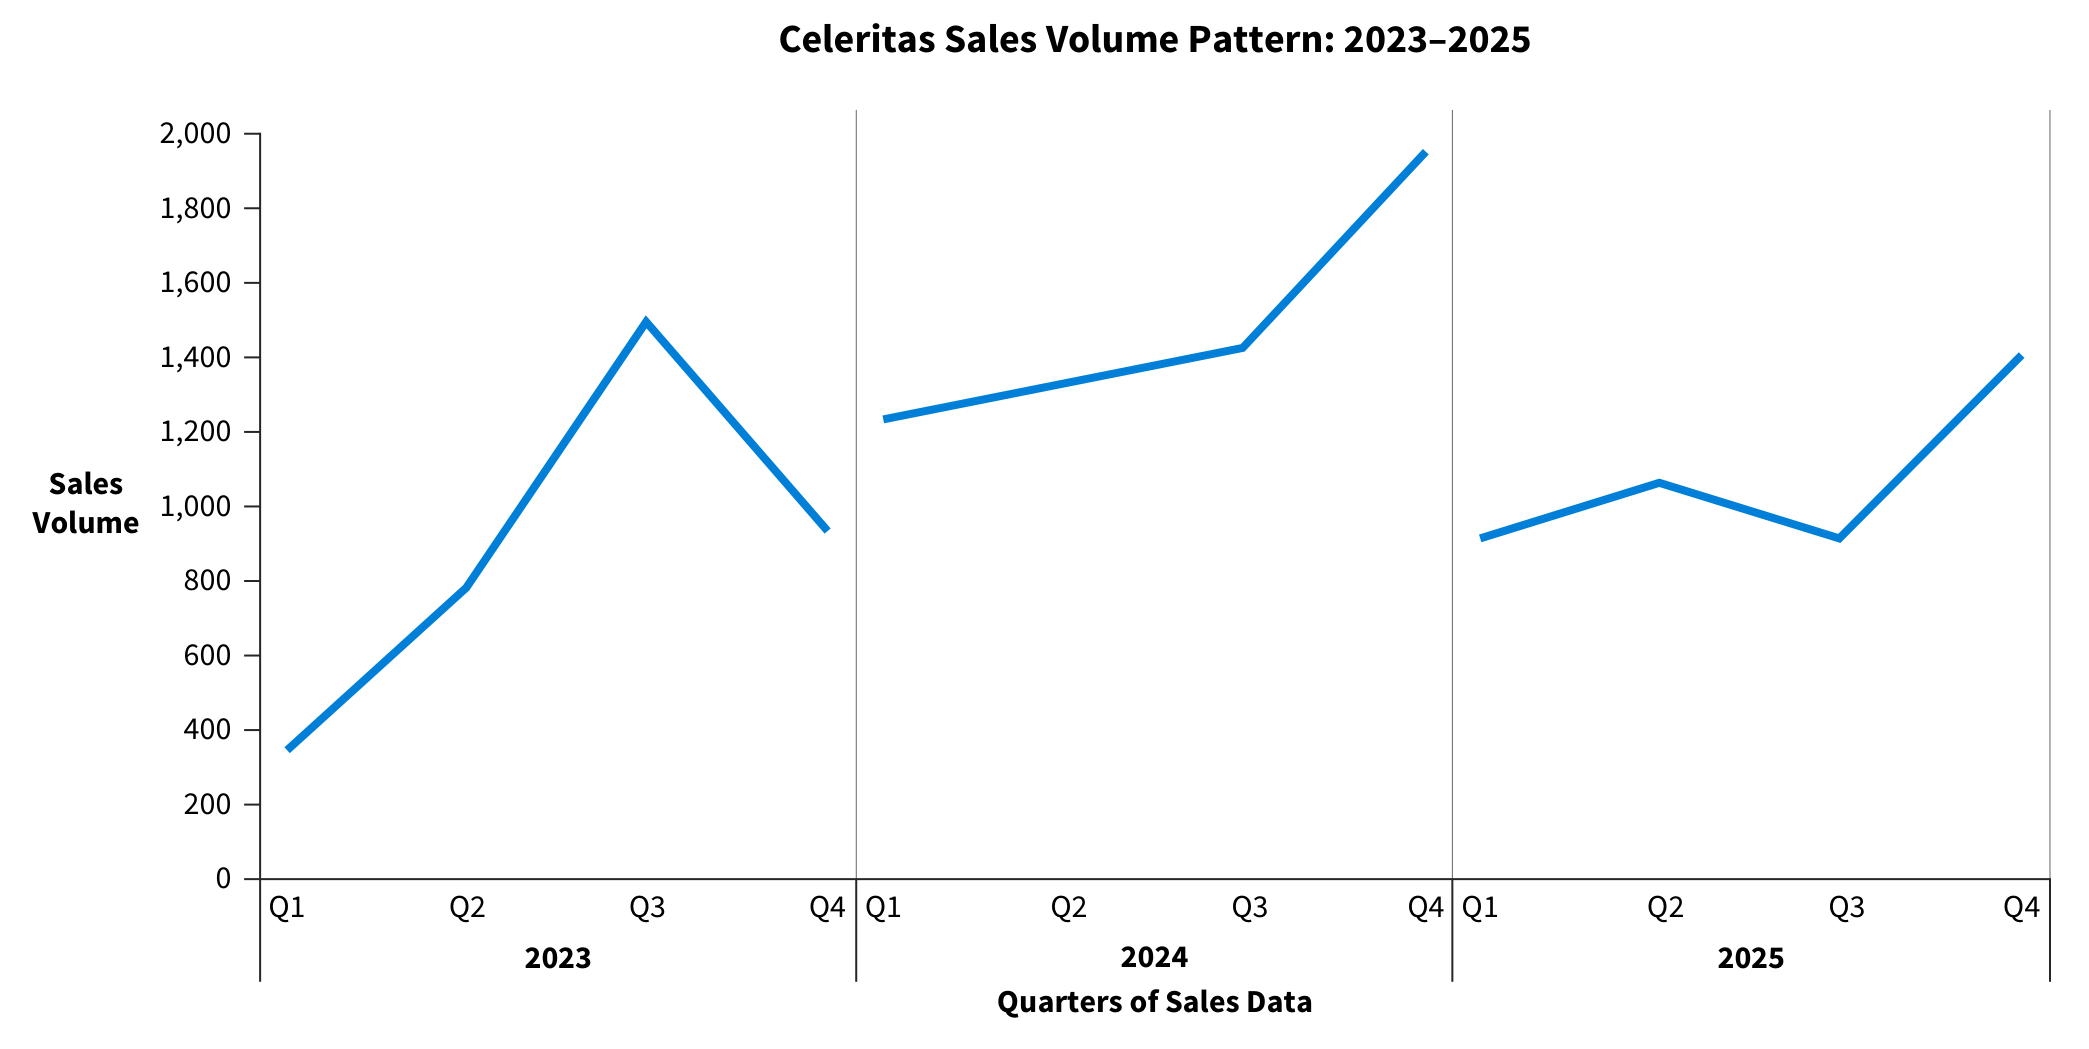
\includegraphics[width=0.95\textwidth,height=0.75\textheight,keepaspectratio]{../textbookForPractice/Figures/Ch_03/ILLUSTRATION 3.12.png}
    \end{figure}
\end{frame}

\begin{frame}{ILLUSTRATION 3.13}

    \begin{figure}[h]
        \centering
        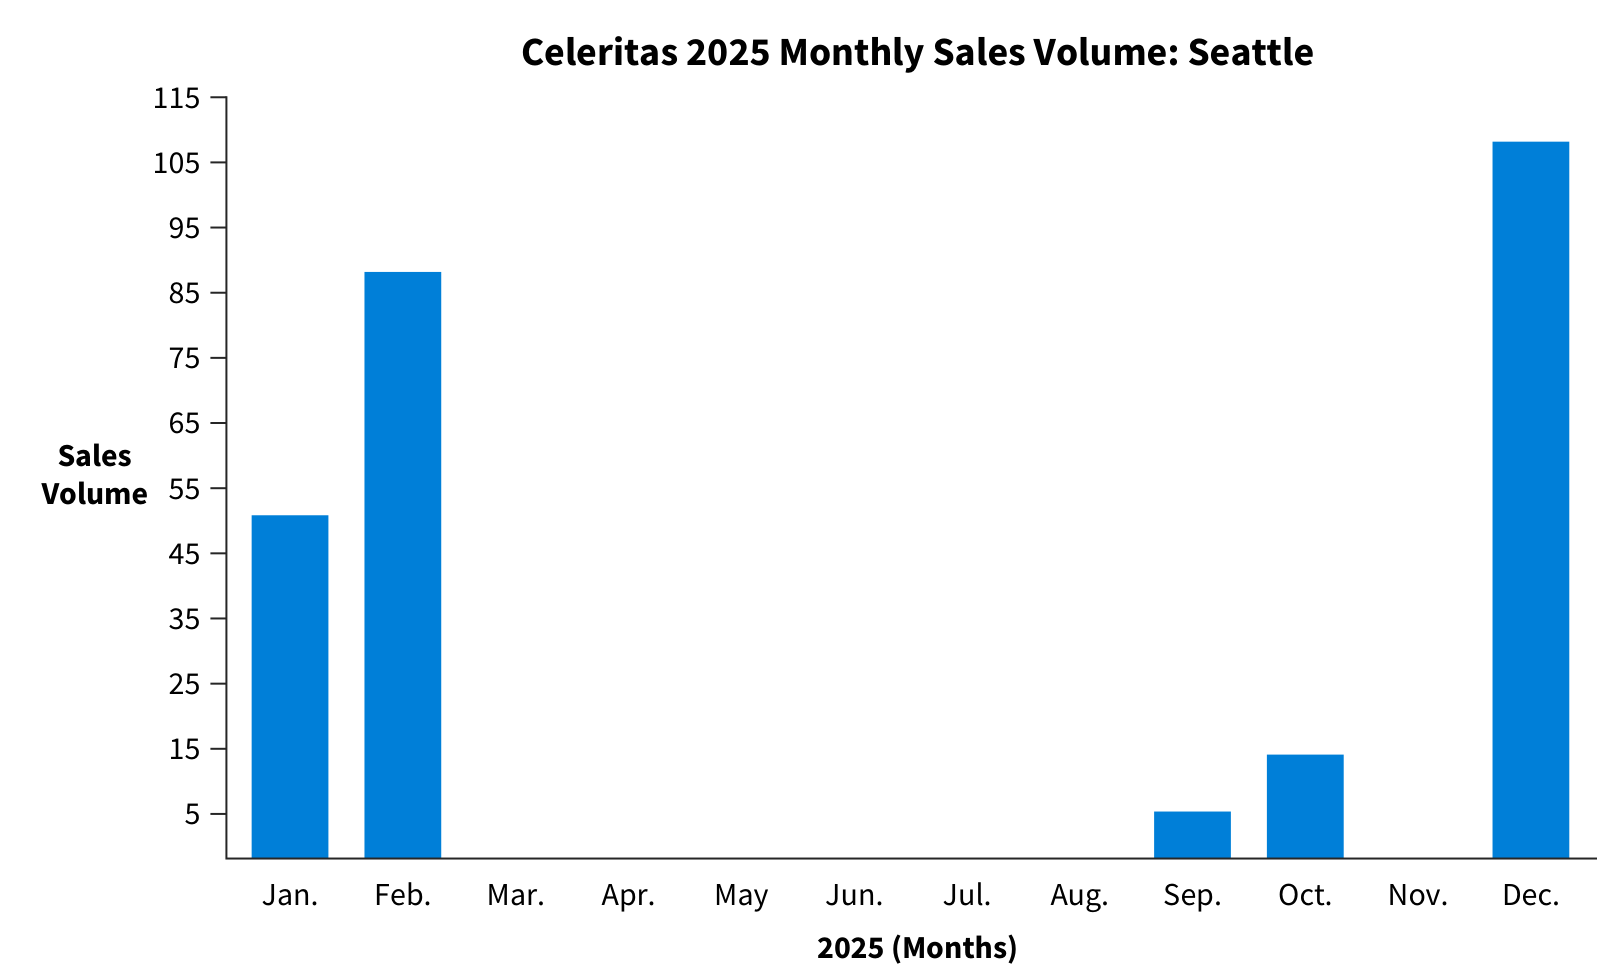
\includegraphics[width=0.95\textwidth,height=0.75\textheight,keepaspectratio]{../textbookForPractice/Figures/Ch_03/ILLUSTRATION 3.13.png}
    \end{figure}
\end{frame}

\begin{frame}{ILLUSTRATION 3.14}

    \begin{figure}[h]
        \centering
        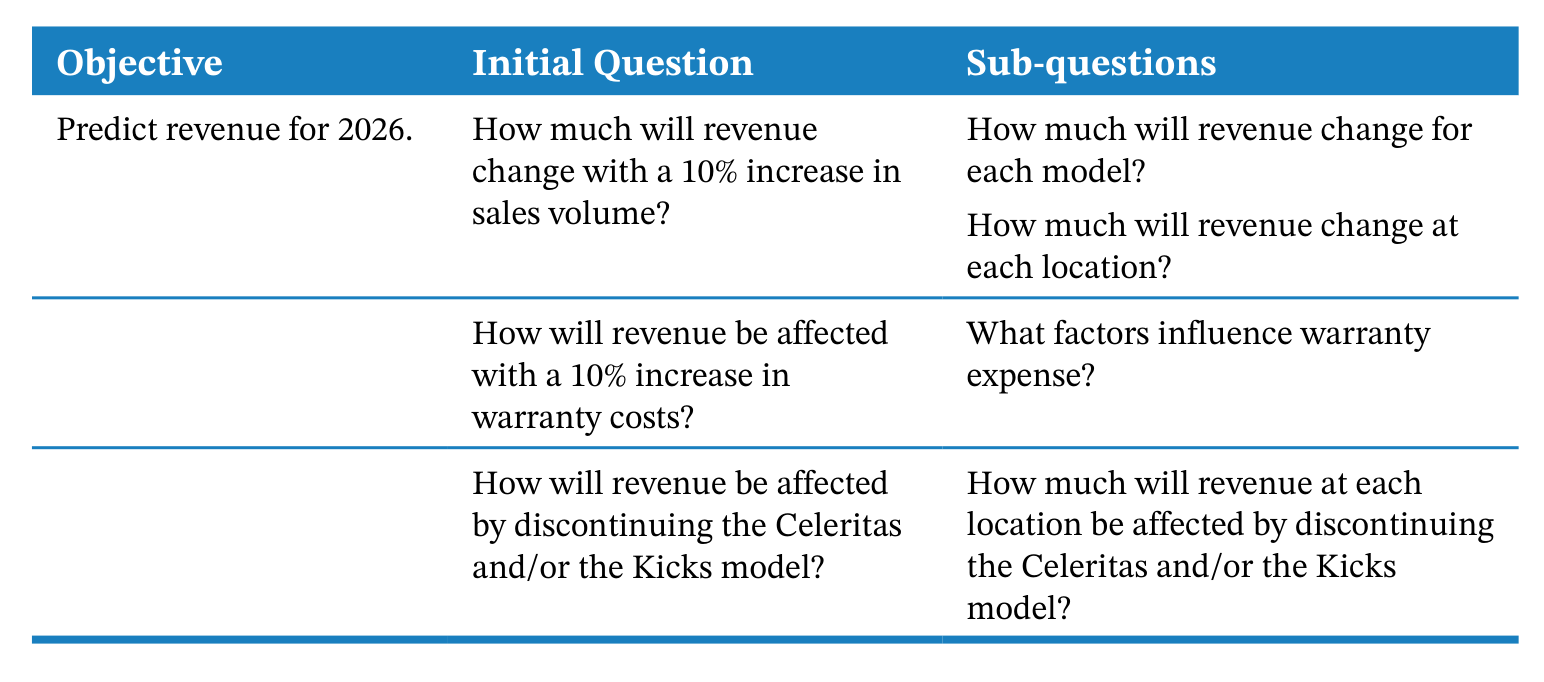
\includegraphics[width=0.95\textwidth,height=0.75\textheight,keepaspectratio]{../textbookForPractice/Figures/Ch_03/ILLUSTRATION 3.14.png}
    \end{figure}
\end{frame}

\begin{frame}{ILLUSTRATION 3.15}

    \begin{figure}[h]
        \centering
        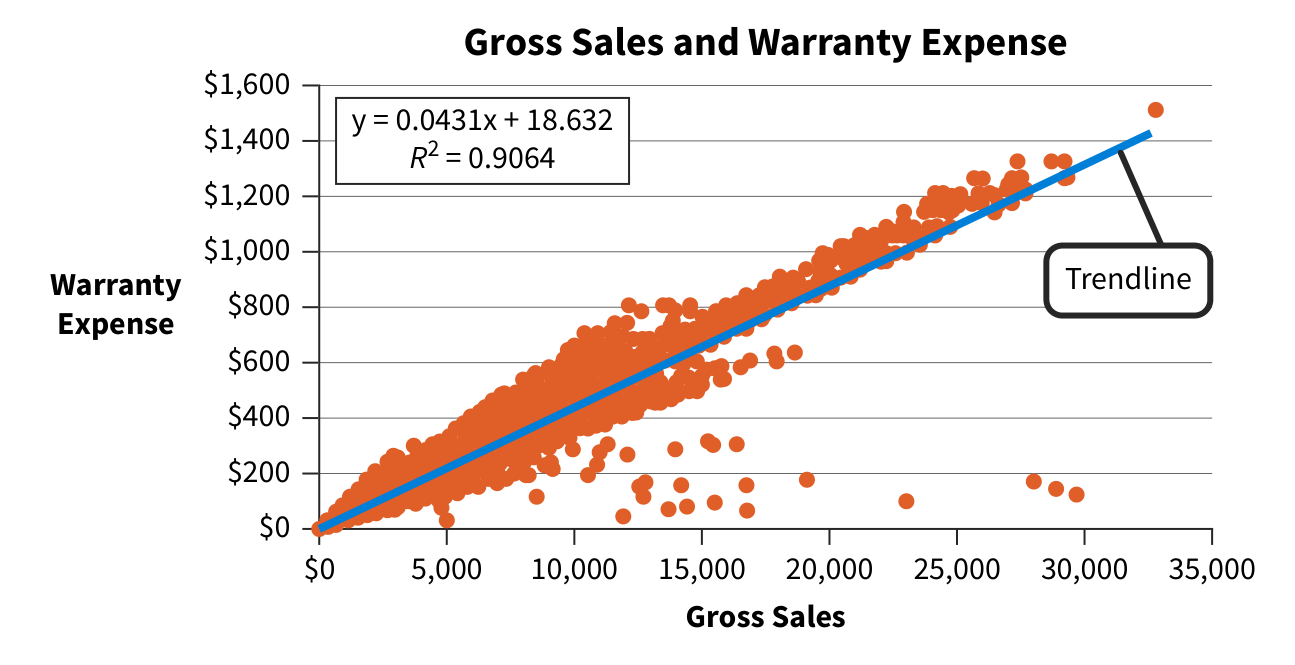
\includegraphics[width=0.95\textwidth,height=0.75\textheight,keepaspectratio]{../textbookForPractice/Figures/Ch_03/ILLUSTRATION 3.15.png}
    \end{figure}
\end{frame}

\begin{frame}{ILLUSTRATION 3.16}

    \begin{figure}[h]
        \centering
        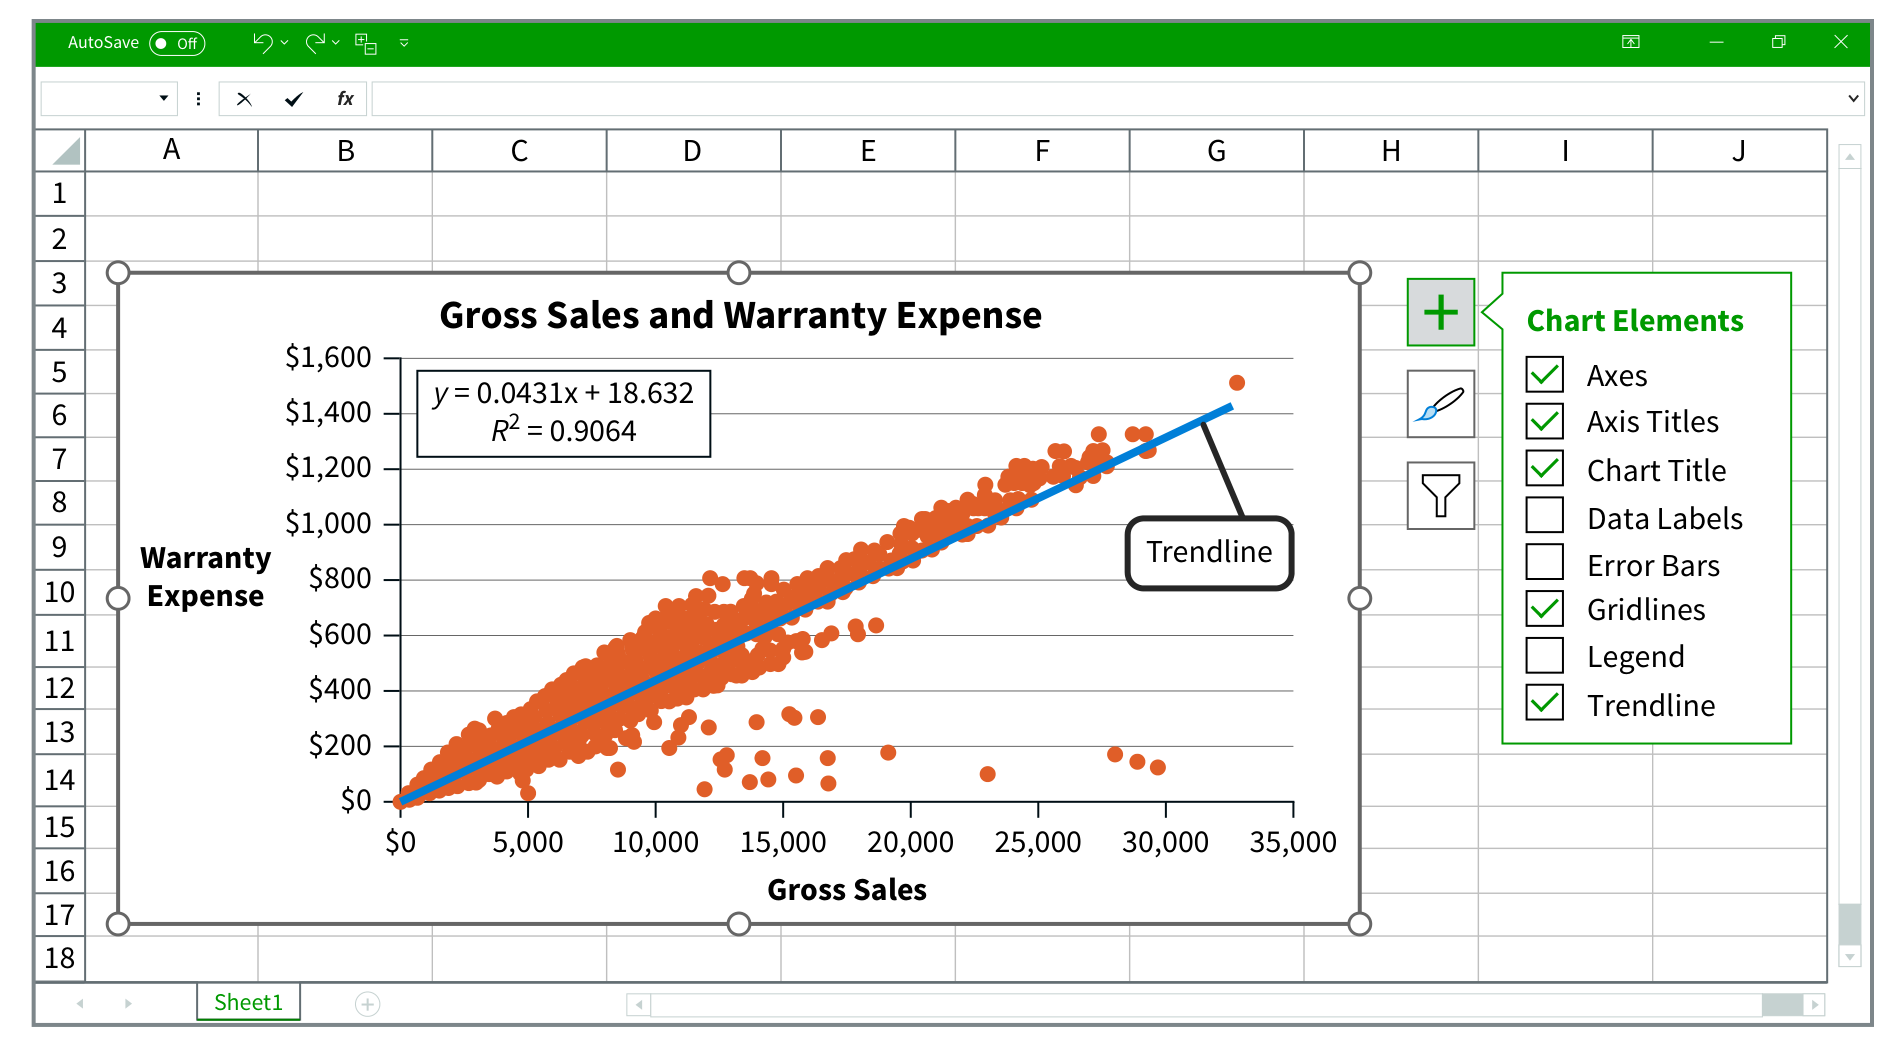
\includegraphics[width=0.95\textwidth,height=0.75\textheight,keepaspectratio]{../textbookForPractice/Figures/Ch_03/ILLUSTRATION 3.16.png}
    \end{figure}
\end{frame}

\begin{frame}{ILLUSTRATION 3.17}

    \begin{figure}[h]
        \centering
        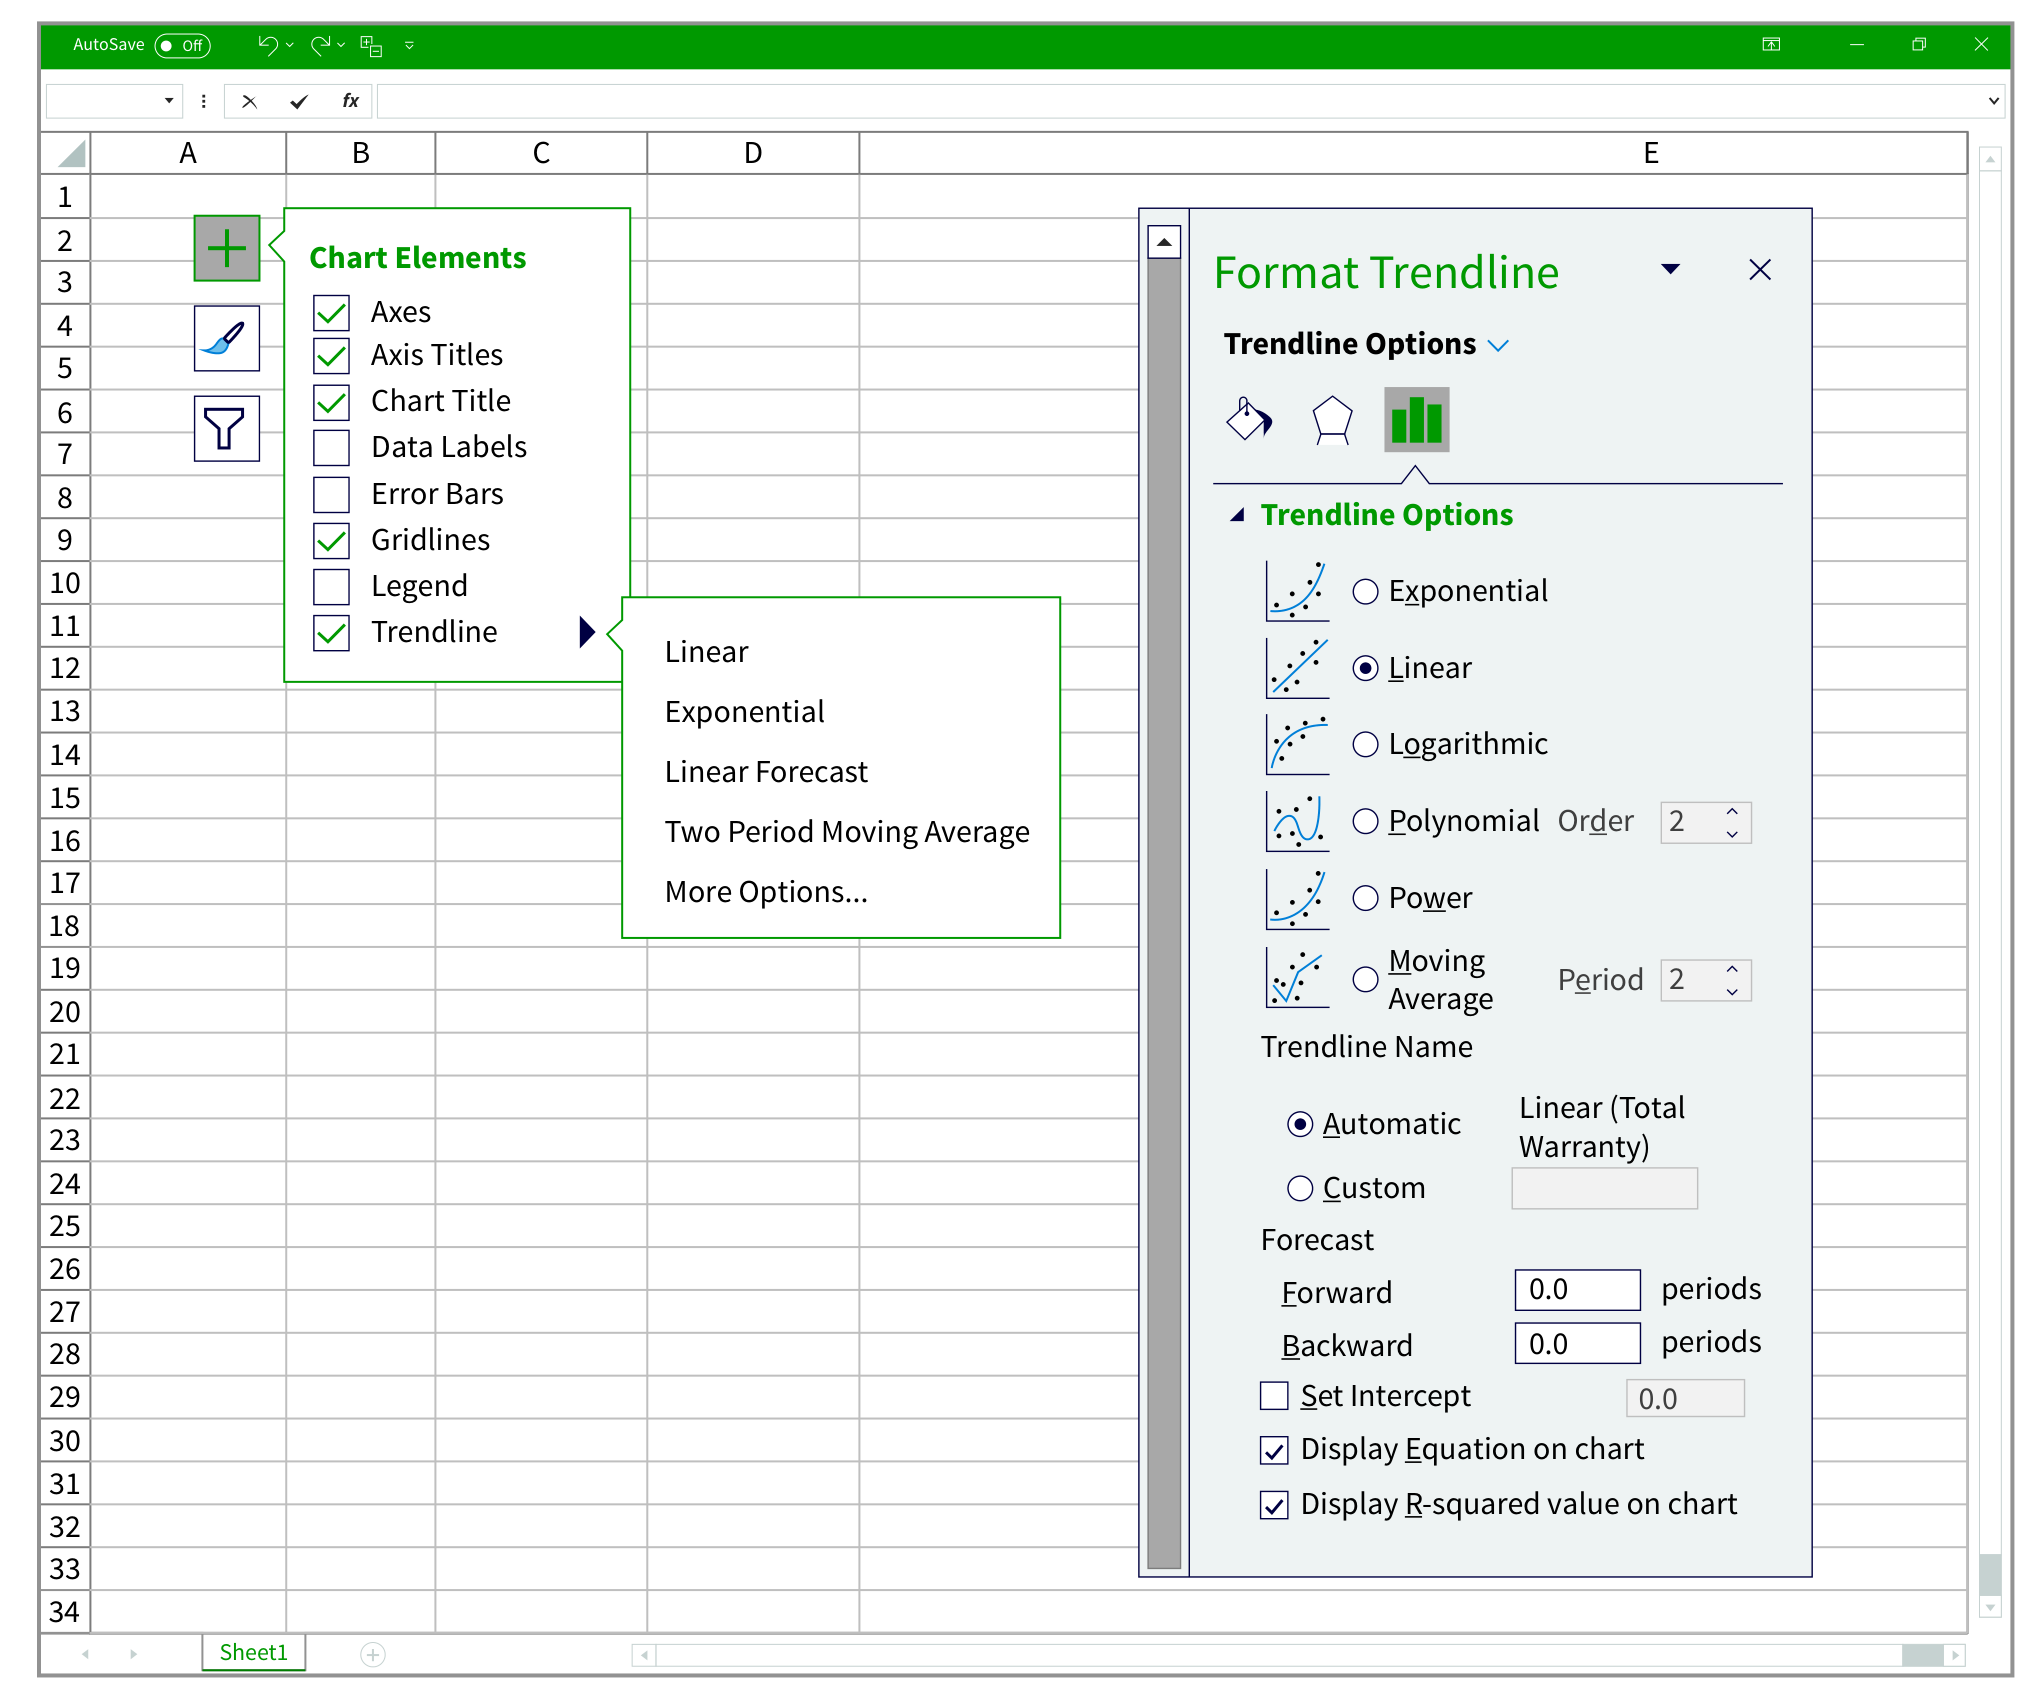
\includegraphics[width=0.95\textwidth,height=0.75\textheight,keepaspectratio]{../textbookForPractice/Figures/Ch_03/ILLUSTRATION 3.17.png}
    \end{figure}
\end{frame}

\begin{frame}{ILLUSTRATION 3.18}

    \begin{figure}[h]
        \centering
        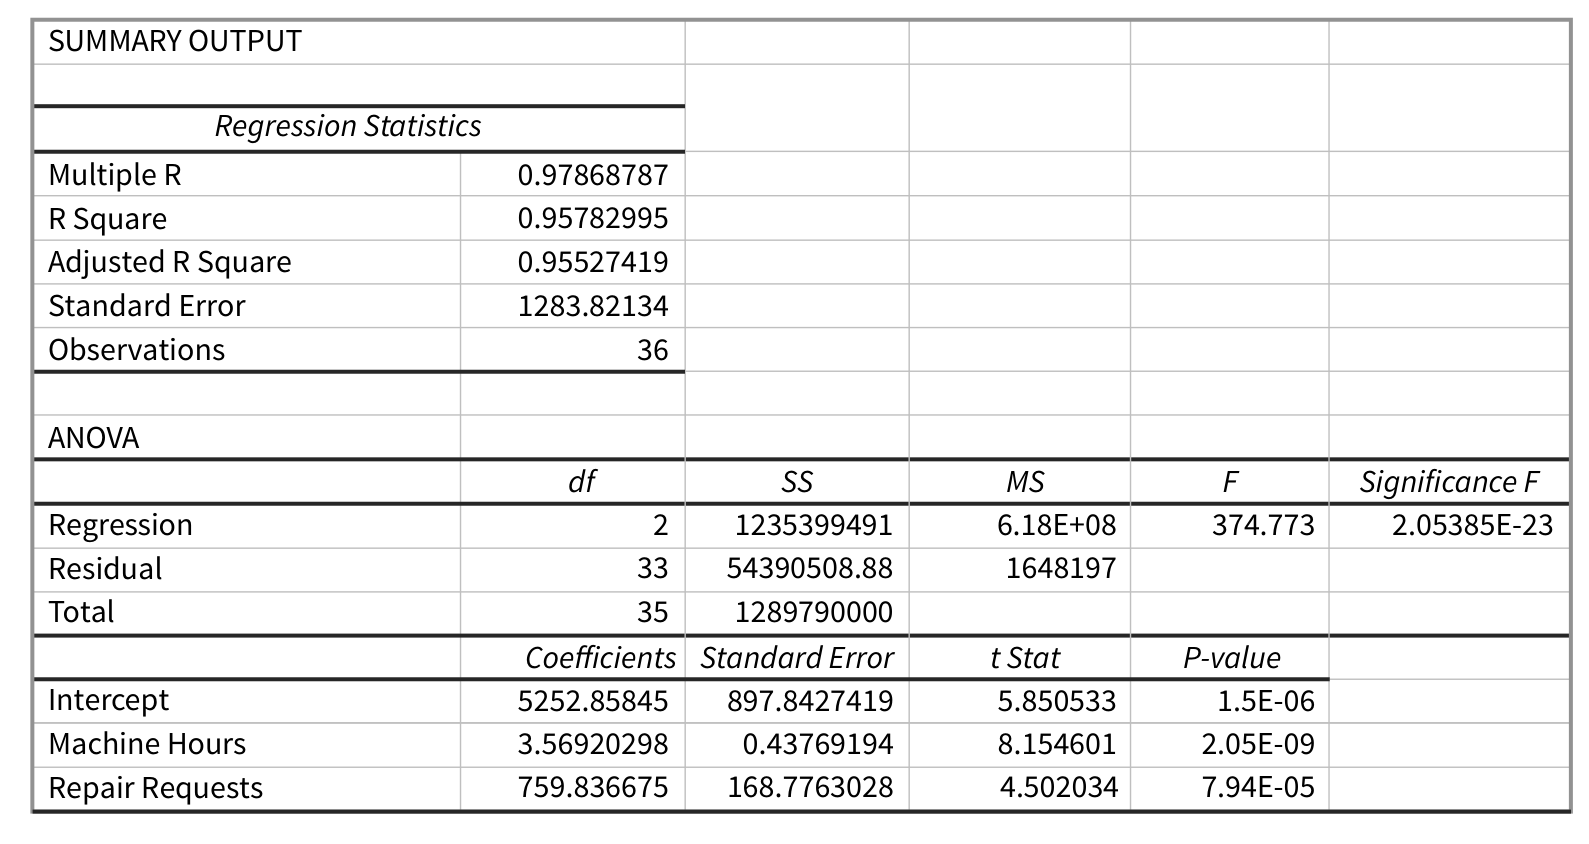
\includegraphics[width=0.95\textwidth,height=0.75\textheight,keepaspectratio]{../textbookForPractice/Figures/Ch_03/ILLUSTRATION 3.18.png}
    \end{figure}
\end{frame}

\begin{frame}{Apply It 3.2}

    \begin{figure}[h]
        \centering
        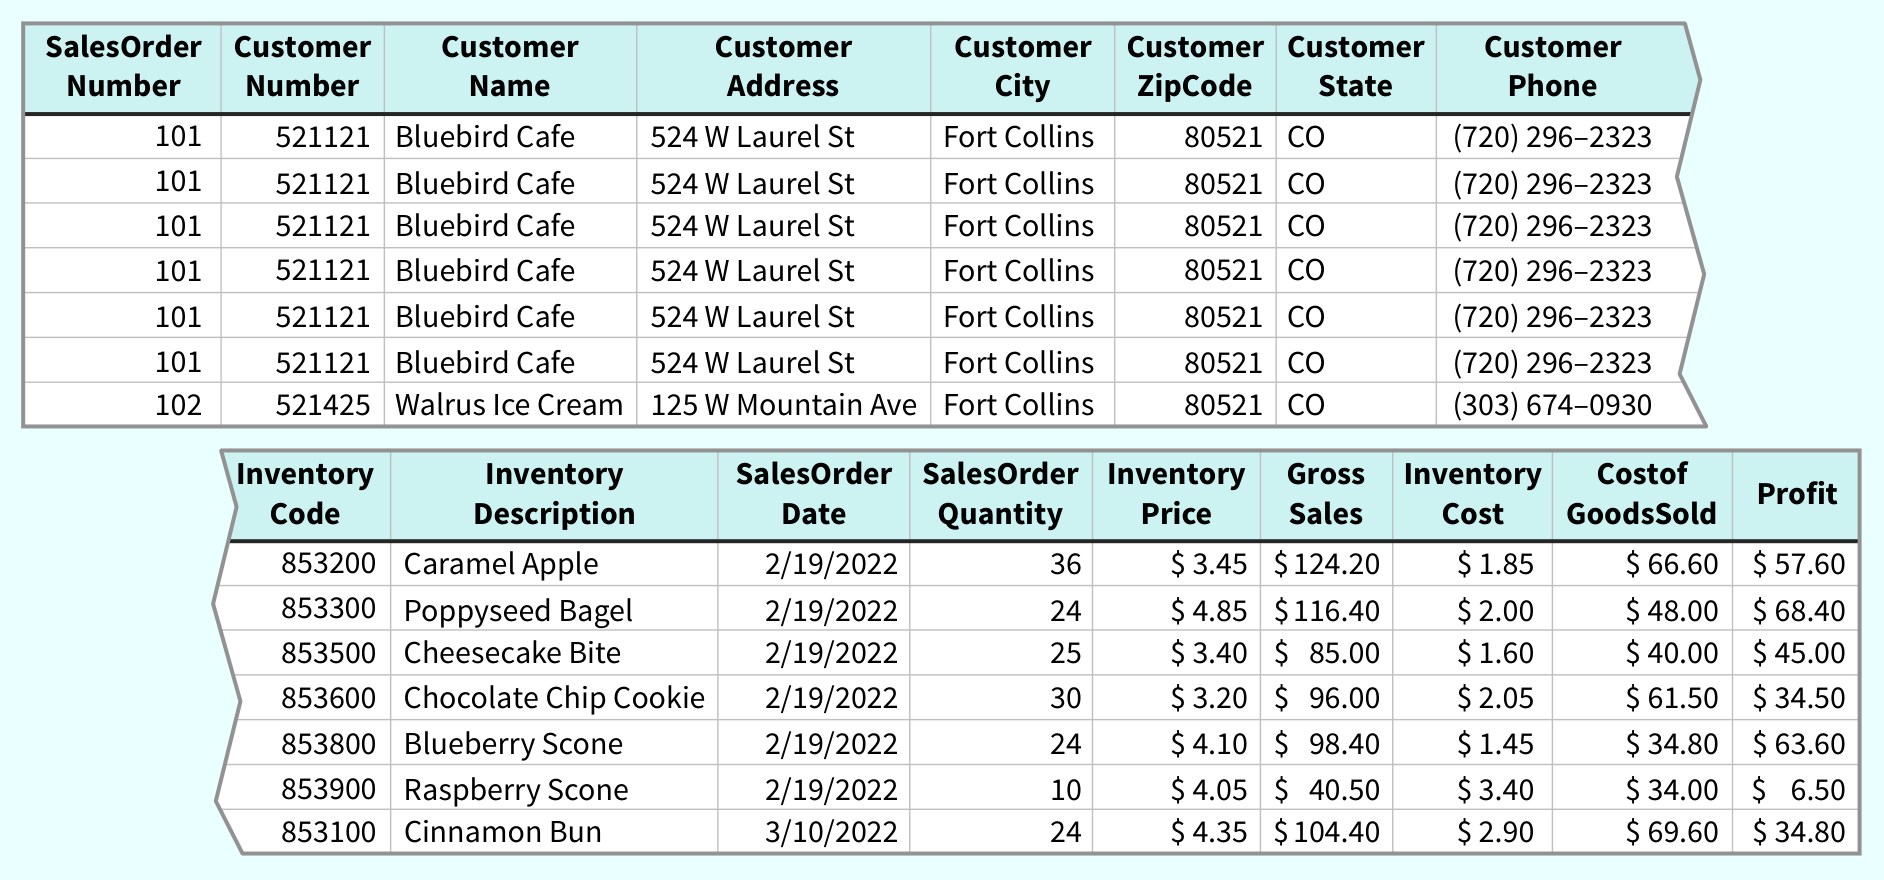
\includegraphics[width=0.95\textwidth,height=0.75\textheight,keepaspectratio]{../textbookForPractice/Figures/Ch_03/Apply It 3.2.png}
    \end{figure}
\end{frame}

\begin{frame}{3.3 Làm thế nào để phát triển Câu hỏi Chẩn đoán?}
\begin{itemize}
    \item \textbf{Câu hỏi Chẩn đoán (Diagnostic Questions):} Bước tiến tiếp theo sau phân tích mô tả. Khi đã biết "điều gì" xảy ra, chúng ta cần tìm hiểu lý do.
    \item \textbf{Trọng tâm cốt lõi:} Tìm câu trả lời cho câu hỏi \textbf{"Tại sao nó lại xảy ra?"} (Why did it happen?).
    \item \textbf{Vai trò:} Đi tìm nguyên nhân gốc rễ (Root Cause Analysis) của các biến động bất thường, các xu hướng hoặc các mô hình ẩn trong dữ liệu kế toán.
\end{itemize}
\end{frame}

\begin{frame}{Đặc điểm của Câu hỏi Chẩn đoán}
\begin{itemize}
    \item \textbf{Phát hiện bất thường (Anomaly Detection):} Tìm kiếm các giá trị ngoại lai (Outliers) có thể là dấu hiệu của sai sót hoặc gian lận.
    \item \textbf{Phân tích tương quan (Correlation Analysis):} Xác định mối quan hệ giữa các biến số (VD: chi phí quảng cáo tăng có thực sự làm tăng doanh thu không?).
    \item \textbf{So sánh (Benchmarking):} So sánh dữ liệu thực tế với ngân sách dự kiến hoặc trung bình ngành để đánh giá chênh lệch.
\end{itemize}
\end{frame}

\begin{frame}{Đào sâu vào Dữ liệu (Drill-down)}
\begin{itemize}
    \item \textbf{Kỹ thuật Drill-down:} Đi từ mức độ tổng hợp cao (High-level summary) xuống mức độ chi tiết (Granular details) để tìm nguyên nhân.
    \item \textbf{Ví dụ:} Nếu biên lợi nhuận gộp toàn công ty giảm, kế toán viên sẽ "drill-down" để xem biên lợi nhuận của từng chi nhánh, sau đó đến từng dòng sản phẩm, và cuối cùng là từng hóa đơn mua nguyên vật liệu.
    \item \textbf{Phân tích đa chiều:} Đánh giá dữ liệu dựa trên nhiều khía cạnh khác nhau như thời gian, địa điểm, sản phẩm.
\end{itemize}
\end{frame}

\begin{frame}{Ví dụ Phân tích Chẩn đoán (Kiểm toán)}
\begin{itemize}
    \item \textbf{Bối cảnh:} Kiểm toán viên phát hiện doanh thu bán hàng trong tháng 12 tăng đột biến 30\% so với trung bình các tháng khác.
    \item \textbf{Câu hỏi Chẩn đoán:} "Tại sao doanh thu lại tăng bất thường vào cuối năm tài chính? Có sự ghi nhận khống doanh thu (Channel Stuffing) không?".
    \item \textbf{Hành động Kiểm toán:} Phân tích chi tiết các bút toán doanh thu cuối tháng, đối chiếu với phiếu xuất kho và chứng từ giao hàng để tìm ra nguyên nhân.
\end{itemize}
\end{frame}

\begin{frame}{Minh họa dữ liệu và trực quan hóa cảnh báo}
\begin{itemize}
    \item \textbf{Bảng điều khiển (Dashboards) cảnh báo:} Các hệ thống phân tích hiện đại có thể tự động highlight các dữ liệu vượt ngưỡng cho phép.
    \item \textbf{Biểu đồ phân tán (Scatter Plot):} Rất hữu ích để phát hiện các giá trị ngoại lai trong hàng triệu giao dịch.
    \item \textbf{Phân tích Benford (Benford's Law):} Ứng dụng trong kiểm toán để trực quan hóa sự phân bố bất thường của các chữ số đầu tiên trong tập dữ liệu kế toán nhằm tìm kiếm dấu hiệu gian lận.
\end{itemize}
\end{frame}

\begin{frame}{ILLUSTRATION 3.19}

    \begin{figure}[h]
        \centering
        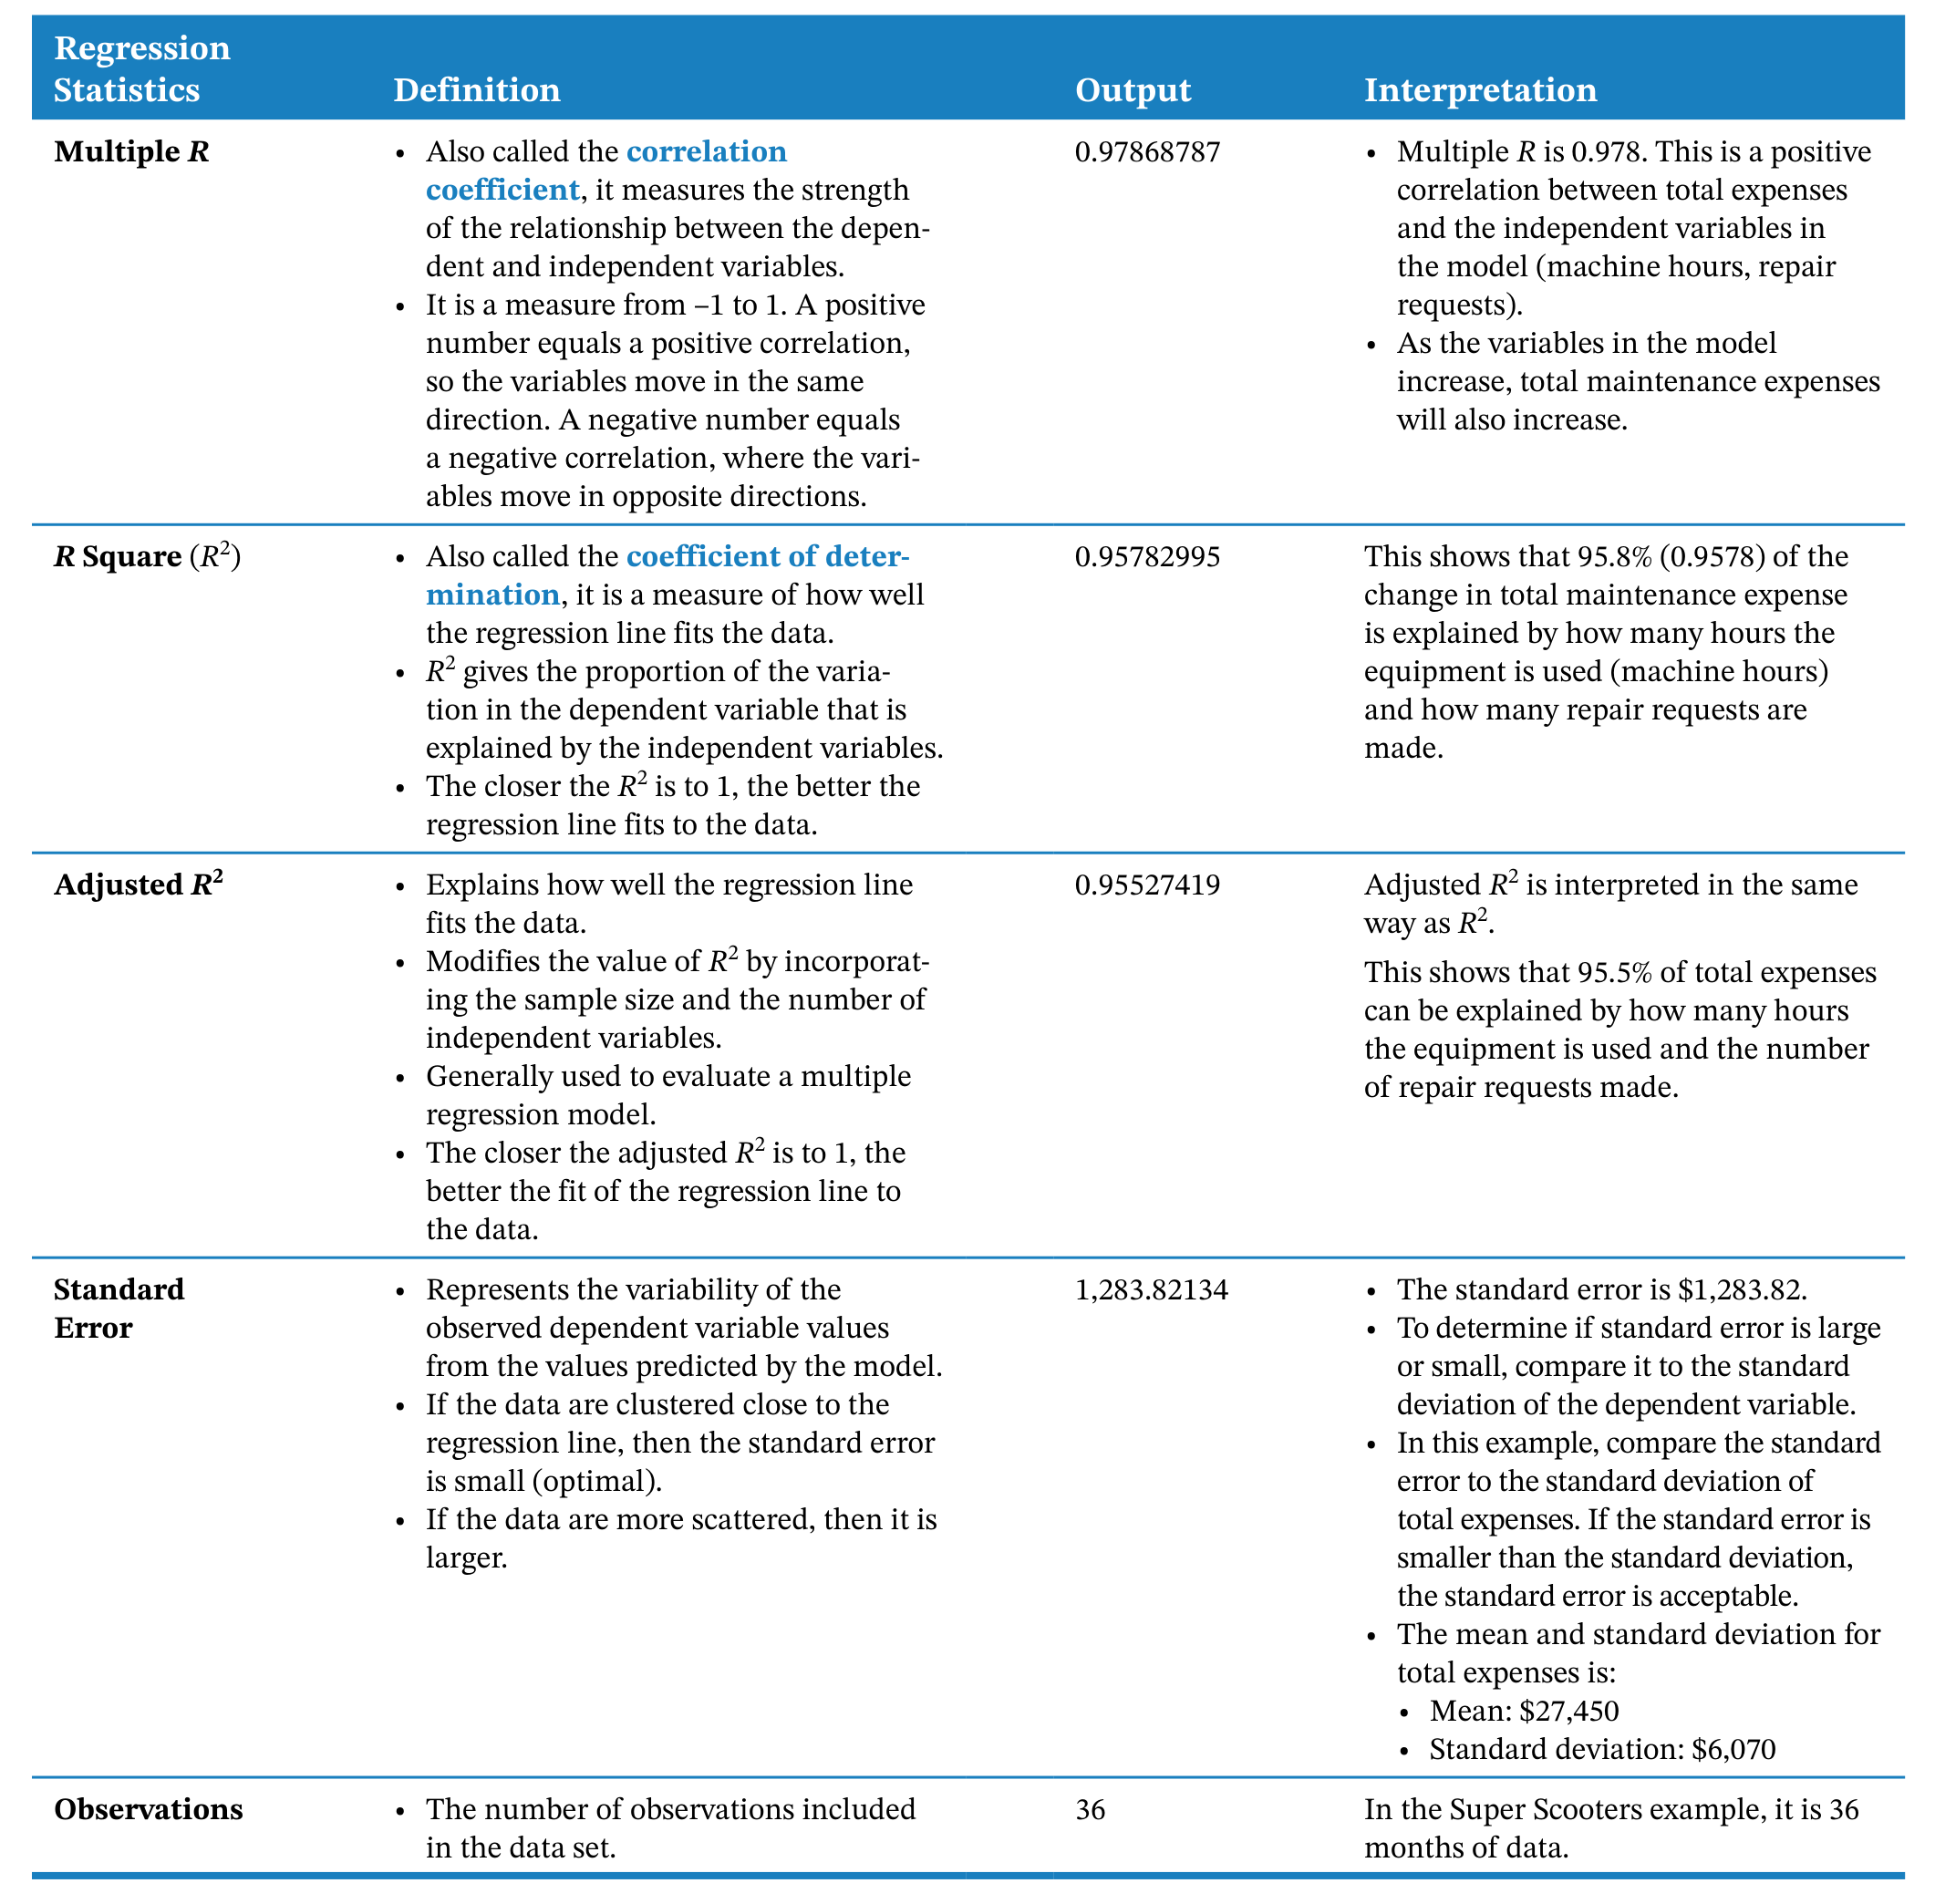
\includegraphics[width=0.95\textwidth,height=0.75\textheight,keepaspectratio]{../textbookForPractice/Figures/Ch_03/ILLUSTRATION 3.19.png}
    \end{figure}
\end{frame}

\begin{frame}{ILLUSTRATION 3.20}

    \begin{figure}[h]
        \centering
        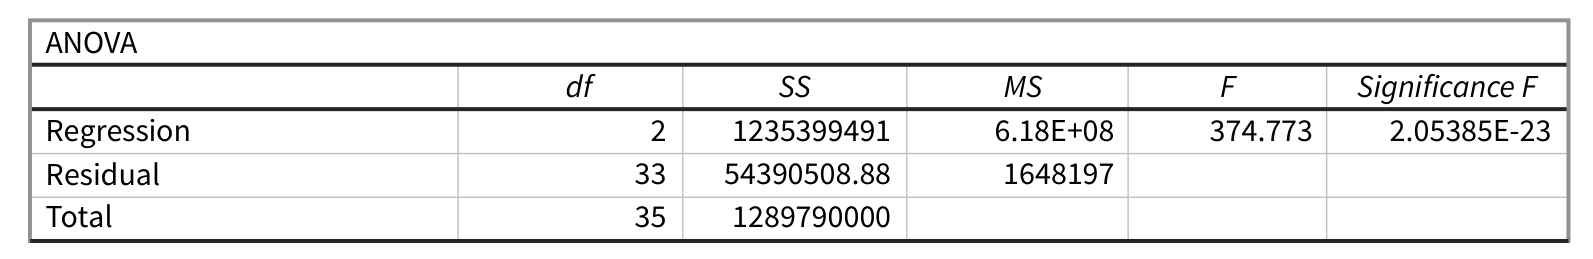
\includegraphics[width=0.95\textwidth,height=0.75\textheight,keepaspectratio]{../textbookForPractice/Figures/Ch_03/ILLUSTRATION 3.20.png}
    \end{figure}
\end{frame}

\begin{frame}{ILLUSTRATION 3.21}

    \begin{figure}[h]
        \centering
        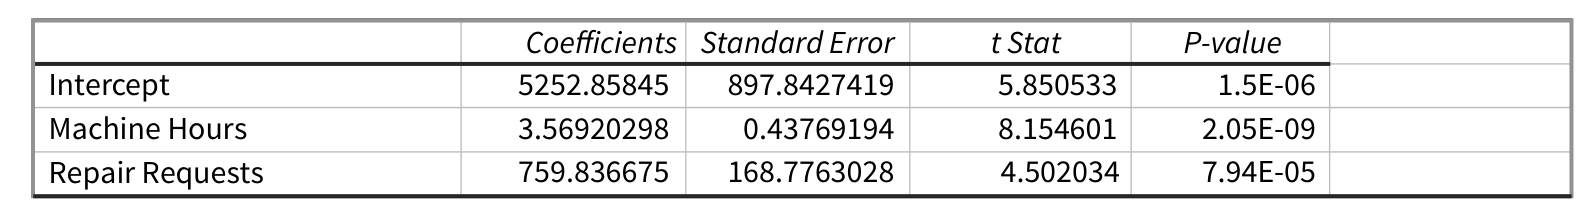
\includegraphics[width=0.95\textwidth,height=0.75\textheight,keepaspectratio]{../textbookForPractice/Figures/Ch_03/ILLUSTRATION 3.21.png}
    \end{figure}
\end{frame}

\begin{frame}{ILLUSTRATION 3.22}

    \begin{figure}[h]
        \centering
        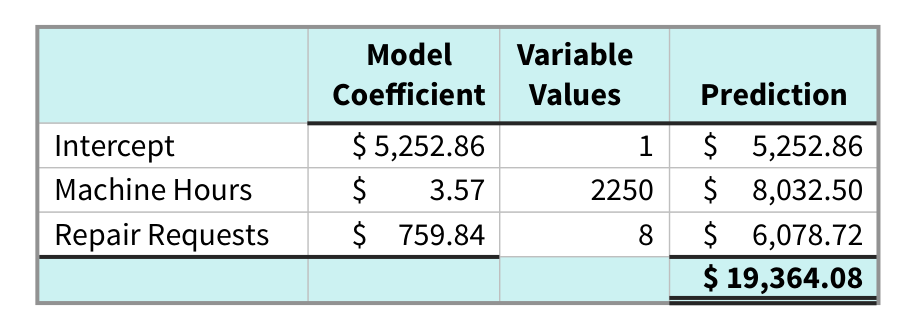
\includegraphics[width=0.95\textwidth,height=0.75\textheight,keepaspectratio]{../textbookForPractice/Figures/Ch_03/ILLUSTRATION 3.22.png}
    \end{figure}
\end{frame}

\begin{frame}{ILLUSTRATION 3.23}

    \begin{figure}[h]
        \centering
        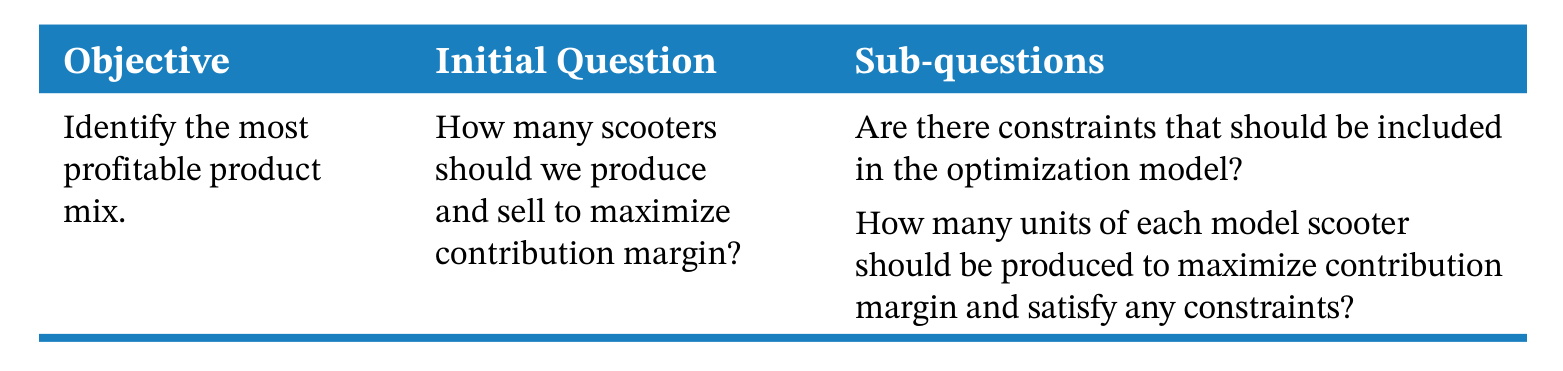
\includegraphics[width=0.95\textwidth,height=0.75\textheight,keepaspectratio]{../textbookForPractice/Figures/Ch_03/ILLUSTRATION 3.23.png}
    \end{figure}
\end{frame}

\begin{frame}{ILLUSTRATION 3.24}

    \begin{figure}[h]
        \centering
        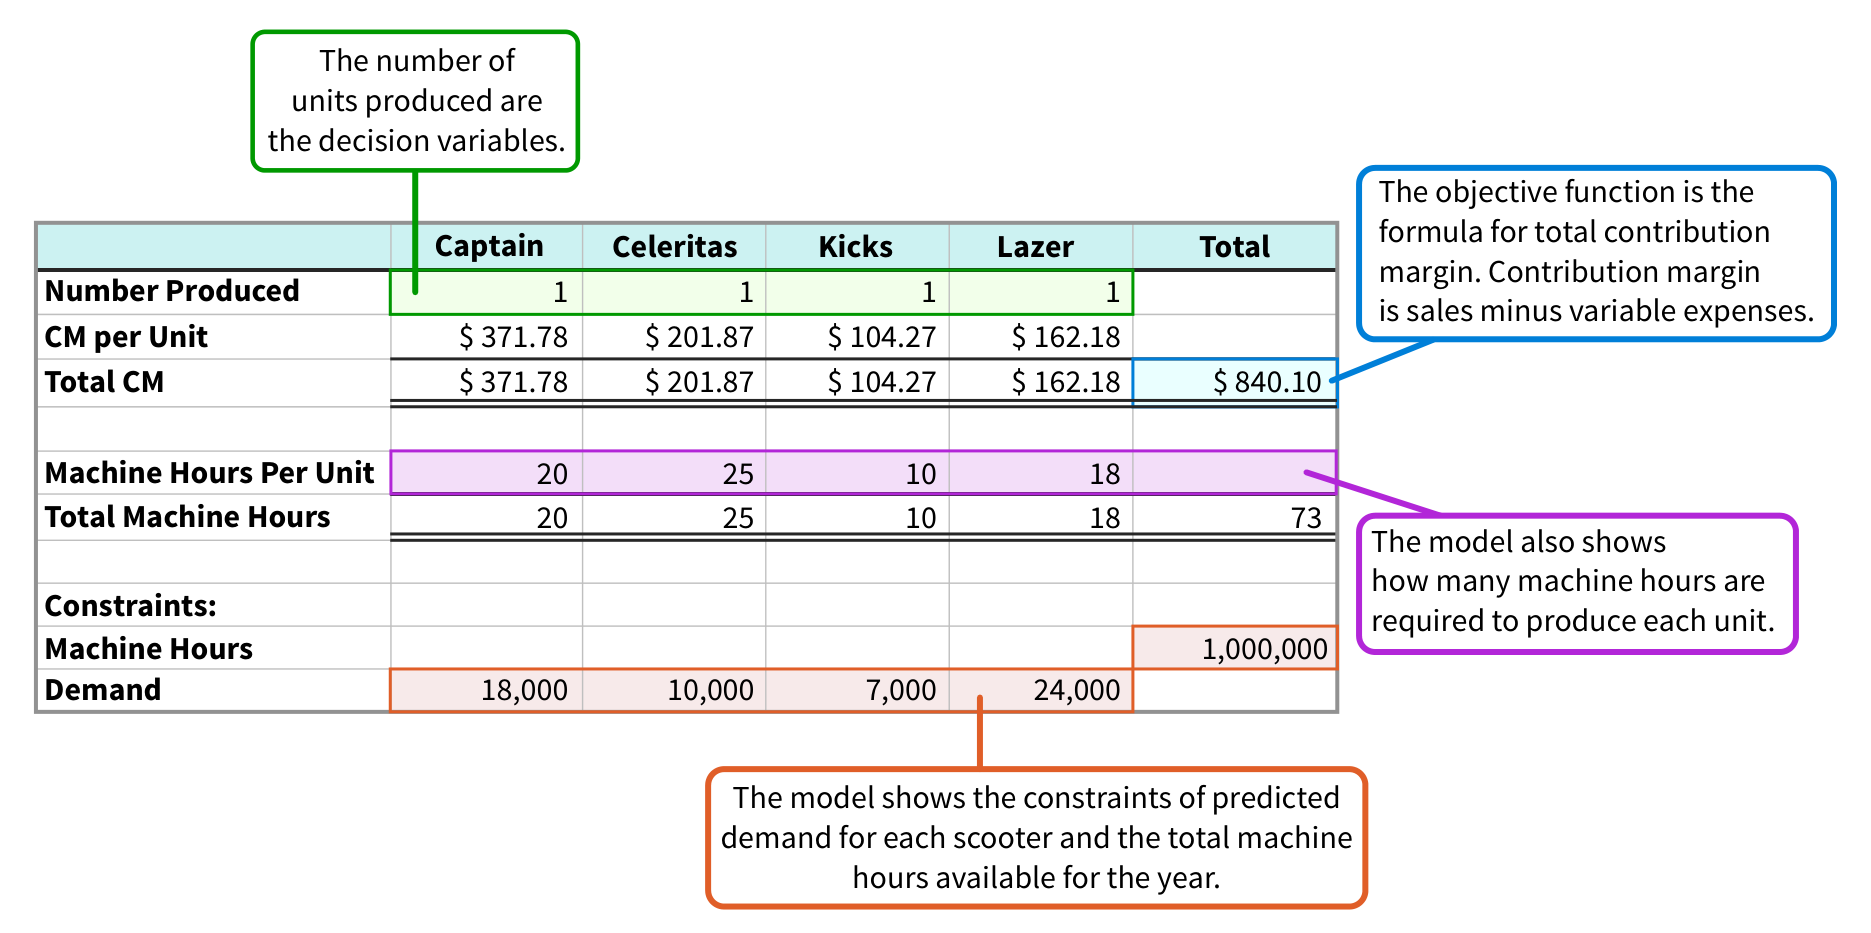
\includegraphics[width=0.95\textwidth,height=0.75\textheight,keepaspectratio]{../textbookForPractice/Figures/Ch_03/ILLUSTRATION 3.24.png}
    \end{figure}
\end{frame}

\begin{frame}{ILLUSTRATION 3.25}

    \begin{figure}[h]
        \centering
        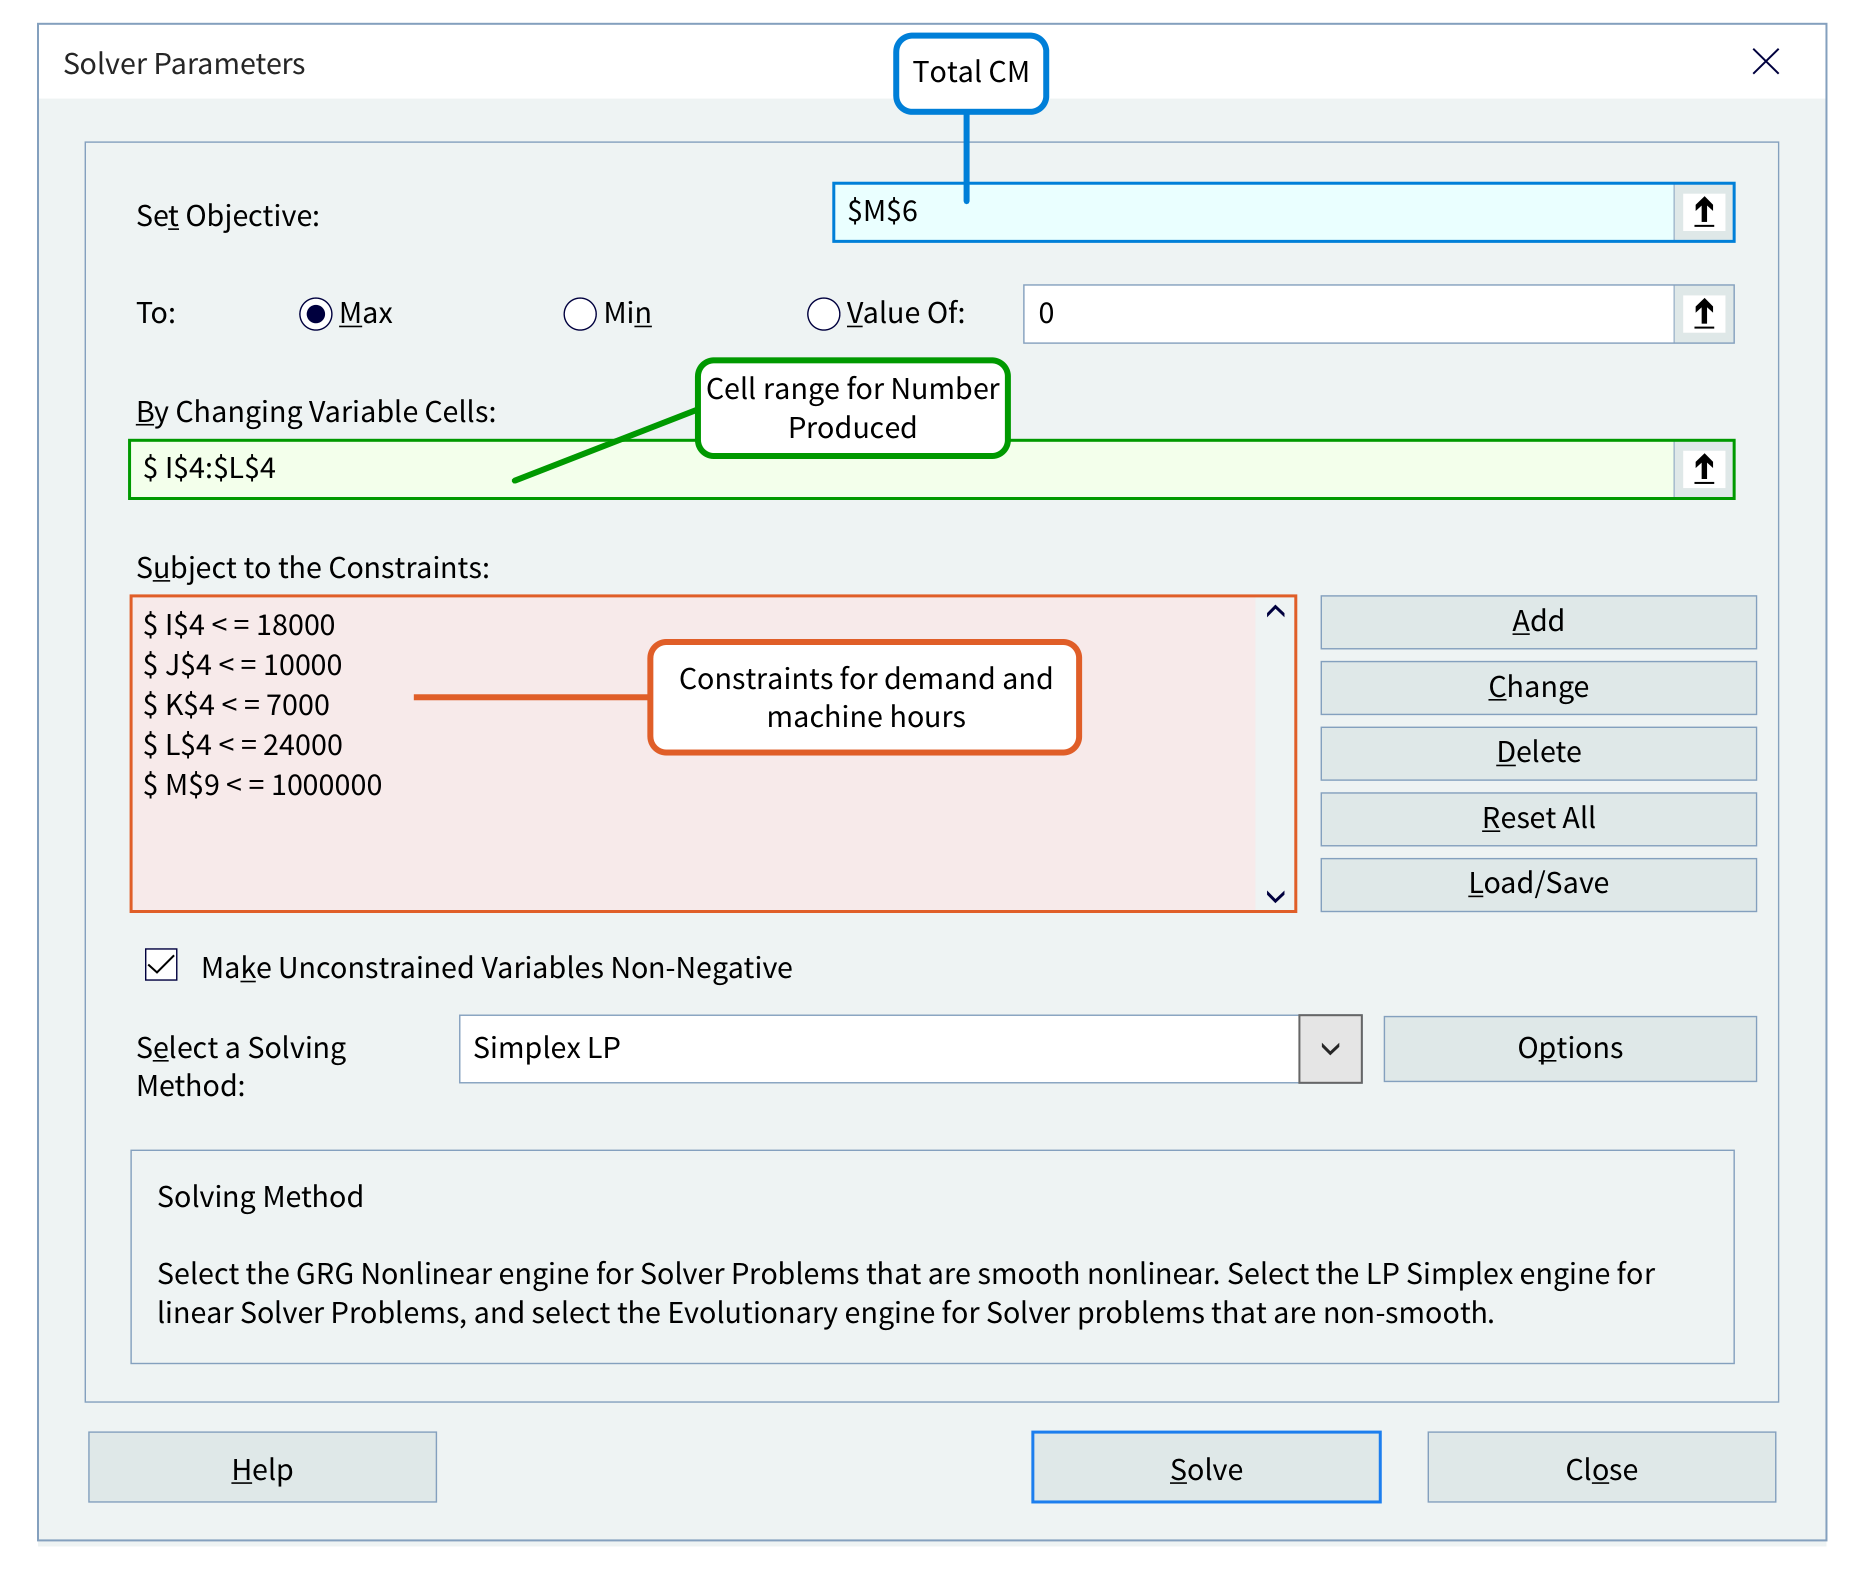
\includegraphics[width=0.95\textwidth,height=0.75\textheight,keepaspectratio]{../textbookForPractice/Figures/Ch_03/ILLUSTRATION 3.25.png}
    \end{figure}
\end{frame}

\begin{frame}{ILLUSTRATION 3.25\_1}

    \begin{figure}[h]
        \centering
        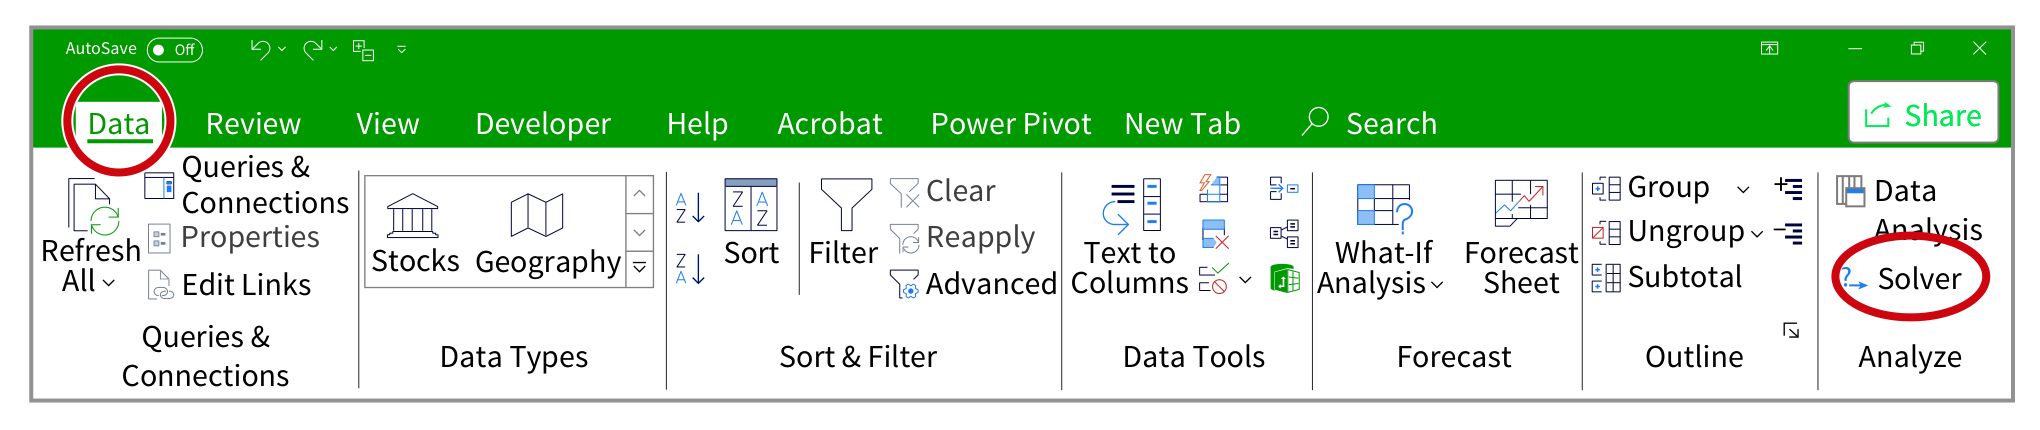
\includegraphics[width=0.95\textwidth,height=0.75\textheight,keepaspectratio]{../textbookForPractice/Figures/Ch_03/ILLUSTRATION 3.25_1.png}
    \end{figure}
\end{frame}

\begin{frame}{ILLUSTRATION 3.26}

    \begin{figure}[h]
        \centering
        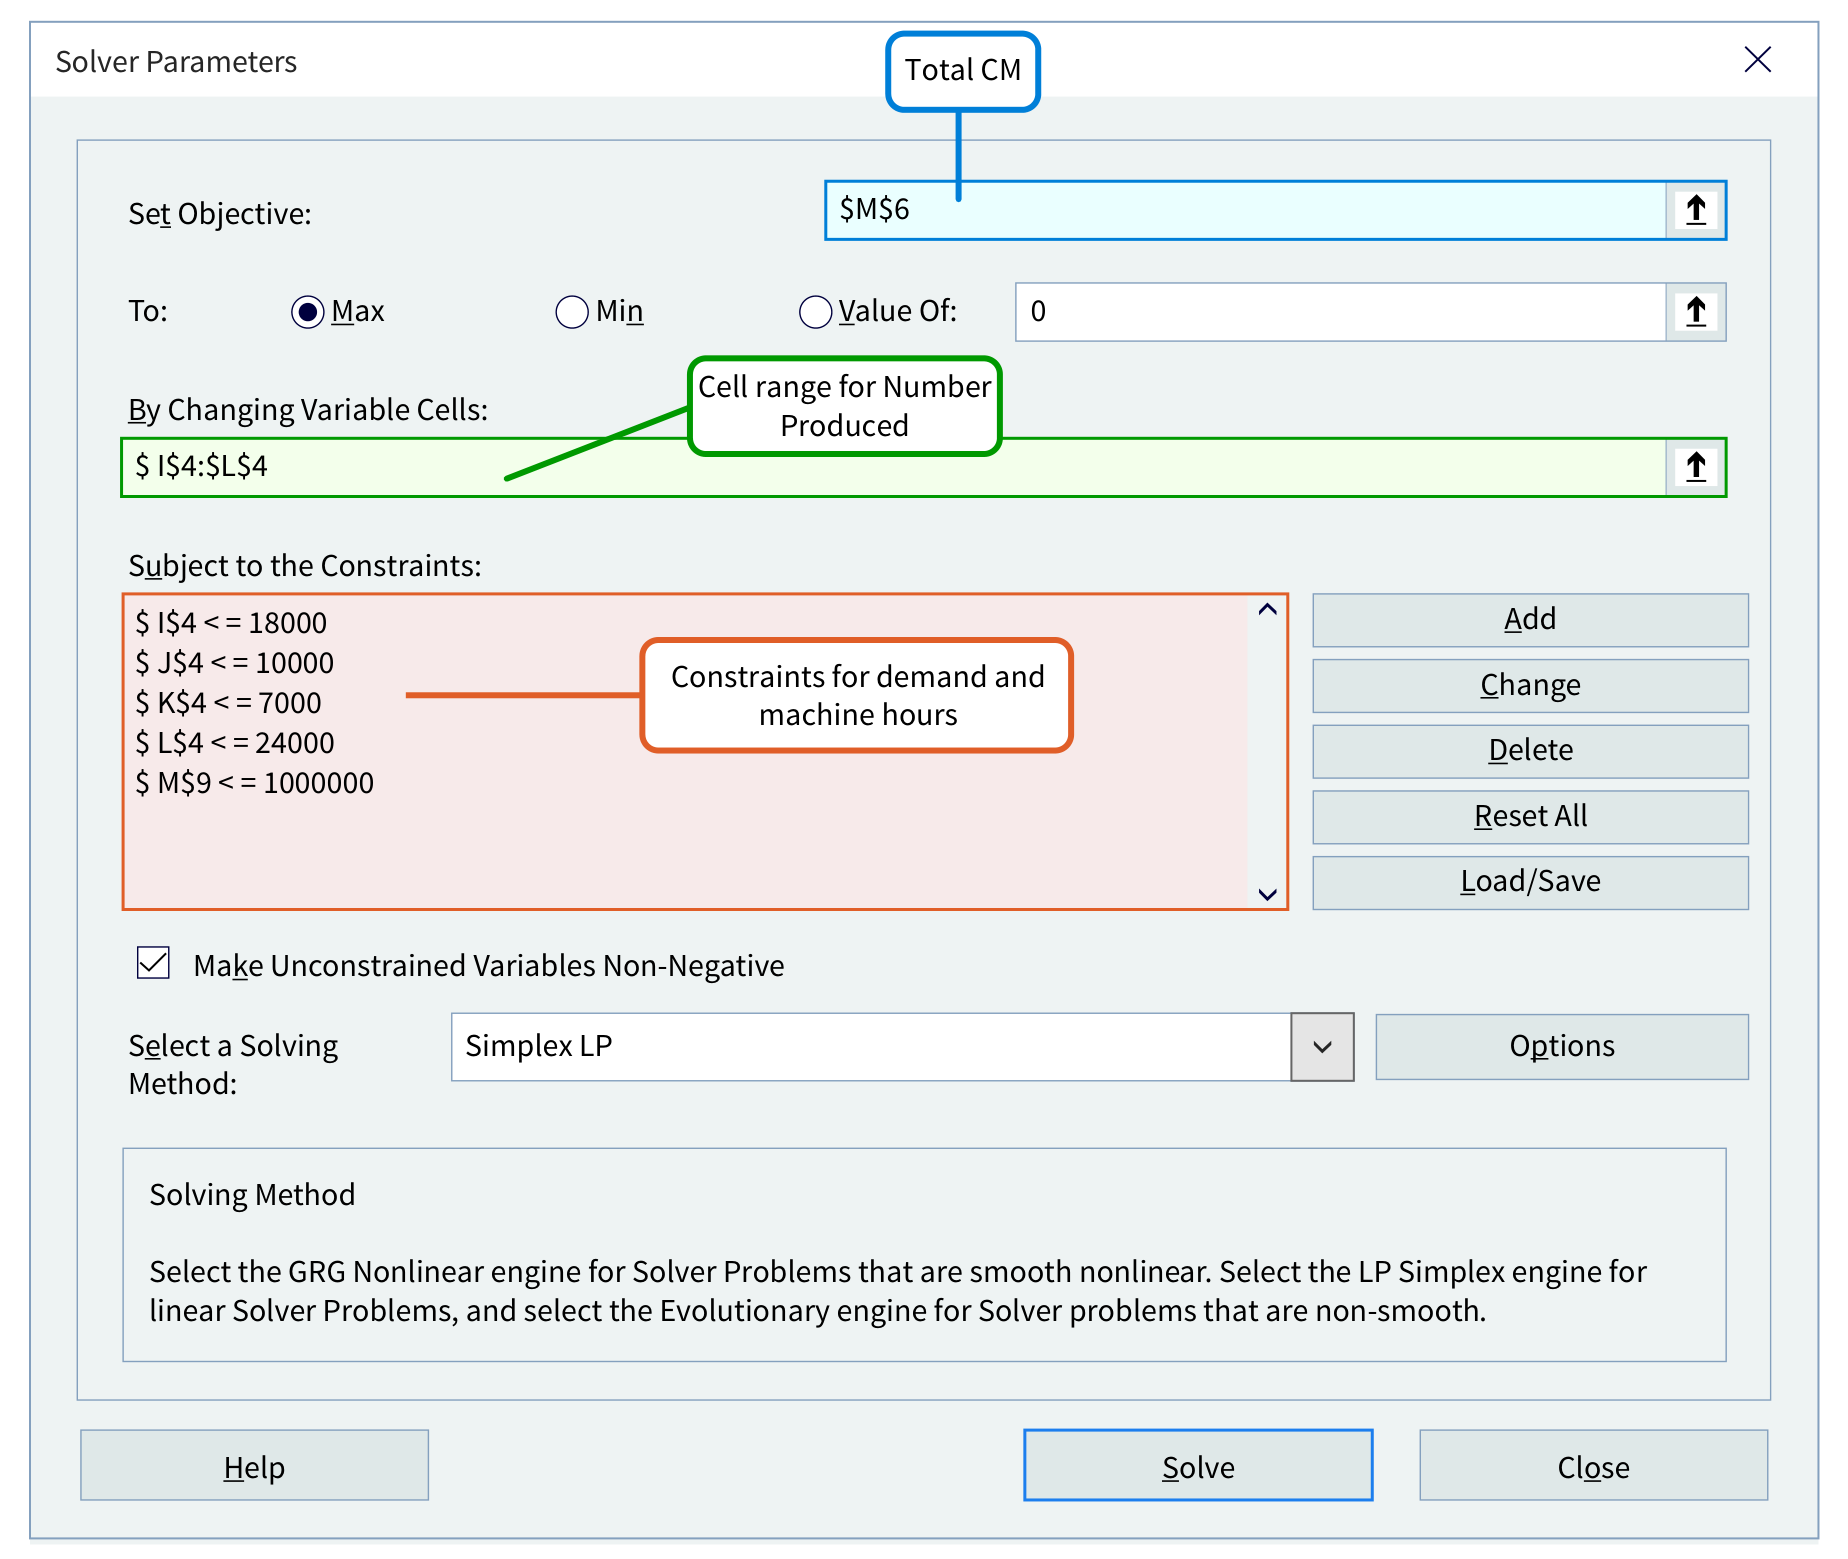
\includegraphics[width=0.95\textwidth,height=0.75\textheight,keepaspectratio]{../textbookForPractice/Figures/Ch_03/ILLUSTRATION 3.26.png}
    \end{figure}
\end{frame}

\begin{frame}{Apply It 3.3}

    \begin{figure}[h]
        \centering
        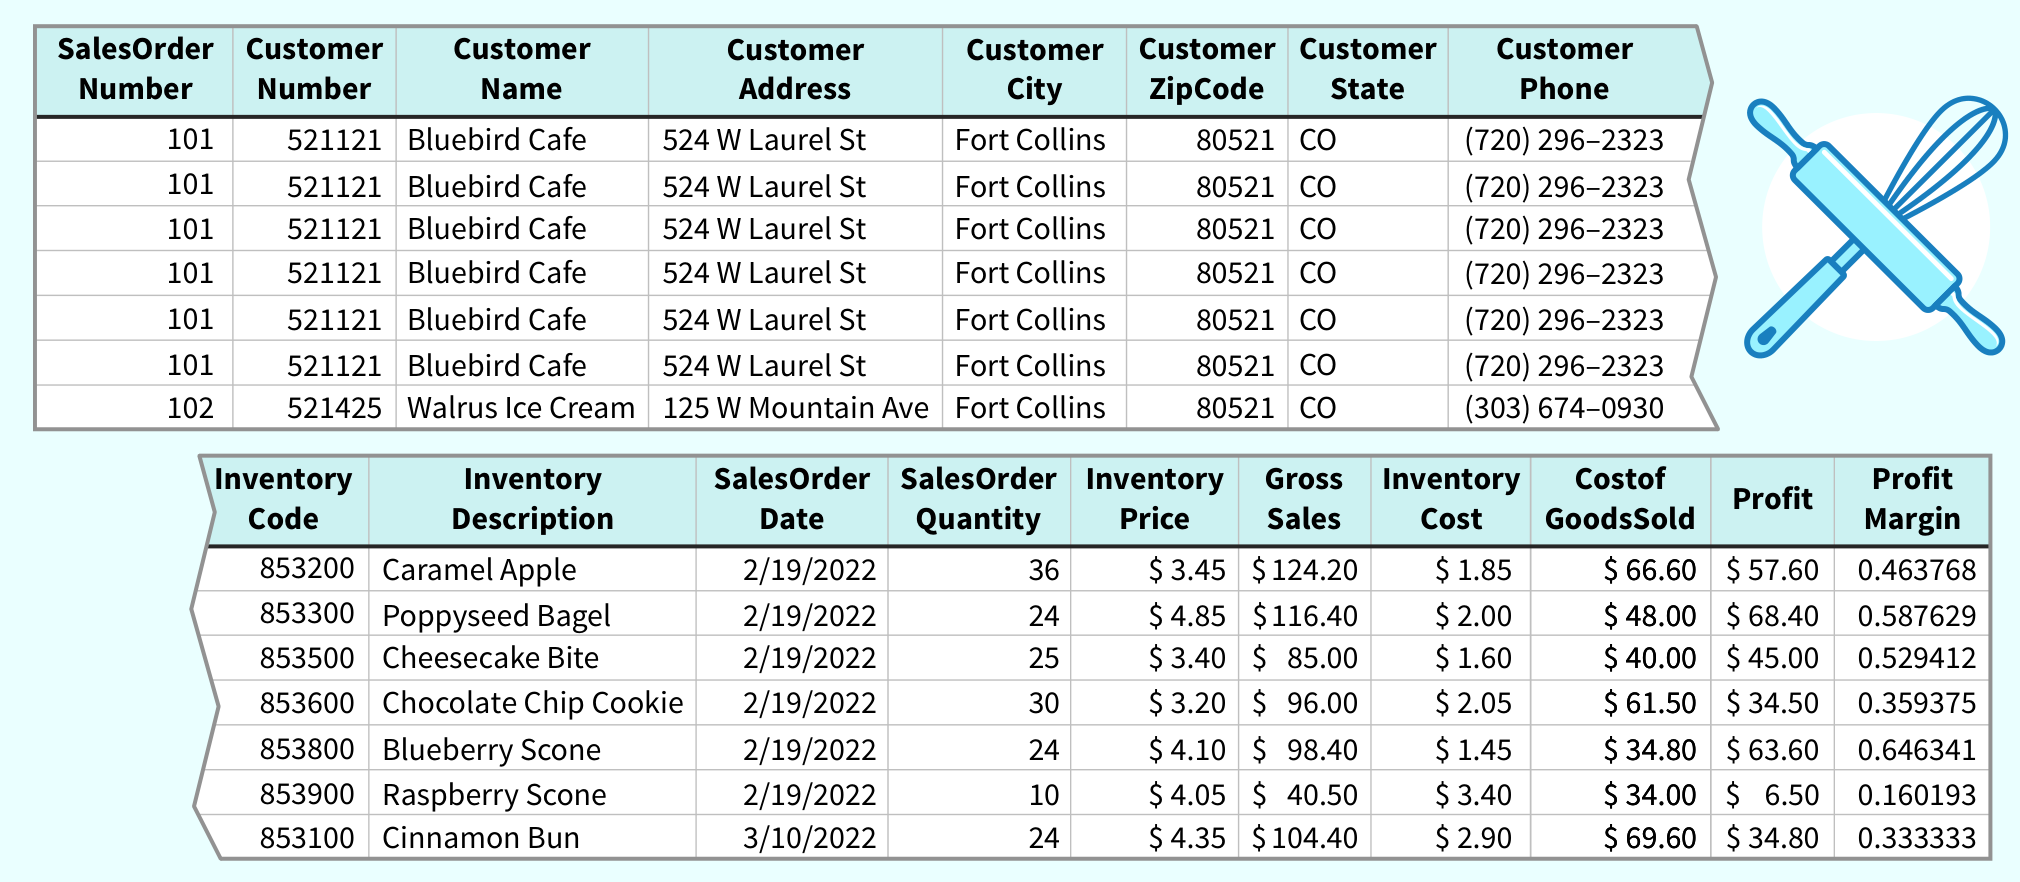
\includegraphics[width=0.95\textwidth,height=0.75\textheight,keepaspectratio]{../textbookForPractice/Figures/Ch_03/Apply It 3.3.png}
    \end{figure}
\end{frame}

\begin{frame}{3.4 Làm thế nào để phát triển Câu hỏi Dự đoán?}
\begin{itemize}
    \item \textbf{Câu hỏi Dự đoán (Predictive Questions):} Sử dụng dữ liệu lịch sử kết hợp với các thuật toán thống kê và học máy (Machine Learning) để hướng về tương lai.
    \item \textbf{Trọng tâm cốt lõi:} Tìm câu trả lời cho câu hỏi \textbf{"Điều gì sẽ xảy ra trong tương lai?"} (What will happen?).
    \item \textbf{Vai trò:} Giúp doanh nghiệp chuyển từ tư duy phản ứng (Reactive) sang tư duy chủ động (Proactive) trong việc lập kế hoạch và quản trị rủi ro.
\end{itemize}
\end{frame}

\begin{frame}{Đặc điểm của Câu hỏi Dự đoán}
\begin{itemize}
    \item \textbf{Xác suất và Rủi ro:} Phân tích dự đoán không cung cấp câu trả lời chắc chắn 100\%, mà nó cung cấp một xác suất về khả năng xảy ra của một sự kiện.
    \item \textbf{Dữ liệu đầu vào:} Đòi hỏi một lượng lớn dữ liệu lịch sử chất lượng cao để "huấn luyện" mô hình dự báo.
    \item \textbf{Ví dụ điển hình:} Dự báo rủi ro phá sản, dự báo dòng tiền tương lai, hoặc đánh giá khả năng vỡ nợ của khách hàng vay tín dụng.
\end{itemize}
\end{frame}

\begin{frame}{Mô hình Phân loại và Dự báo}
\begin{itemize}
    \item \textbf{Phân loại (Classification):} Dự đoán biến phụ thuộc mang tính phân loại. VD: Khách hàng này "Có khả năng vỡ nợ" hay "Không vỡ nợ"? Giao dịch này là "Gian lận" hay "Hợp lệ"?
    \item \textbf{Dự báo (Forecasting):} Dự đoán biến phụ thuộc mang tính liên tục (số lượng). VD: Doanh thu tháng tới sẽ đạt bao nhiêu tỷ đồng?
    \item \textbf{Hồi quy (Regression):} Phương pháp thống kê phổ biến để dự đoán giá trị liên tục dựa trên mối quan hệ giữa các biến độc lập và biến phụ thuộc.
\end{itemize}
\end{frame}

\begin{frame}{Ví dụ Phân tích Dự đoán (Kế toán Quản trị)}
\begin{itemize}
    \item \textbf{Bối cảnh:} Quản lý sản xuất muốn lên kế hoạch nhập nguyên vật liệu cho quý 3.
    \item \textbf{Câu hỏi Dự đoán:} "Sản lượng bán ra của sản phẩm A trong tháng 7, 8 và 9 dự kiến là bao nhiêu dựa trên xu hướng bán hàng của 3 năm qua và các yếu tố kinh tế vĩ mô?".
    \item \textbf{Hành động:} Kế toán quản trị xây dựng mô hình phân tích chuỗi thời gian (Time-series analysis) để dự báo nhu cầu thị trường, từ đó tối ưu hóa chi phí tồn kho.
\end{itemize}
\end{frame}

\begin{frame}{Đánh giá xu hướng chuỗi thời gian}
\begin{itemize}
    \item \textbf{Chuỗi thời gian (Time Series):} Là một chuỗi các điểm dữ liệu được thu thập theo các khoảng thời gian đều đặn (như theo ngày, tuần, tháng).
    \item \textbf{Thành phần của xu hướng:} Bao gồm Xu hướng chung (Trend), Tính mùa vụ (Seasonality), Tính chu kỳ (Cyclicality) và Biến động ngẫu nhiên (Noise).
    \item \textbf{Ứng dụng thực tiễn:} Loại bỏ yếu tố mùa vụ để dự đoán chính xác tốc độ tăng trưởng doanh thu thực sự của một mảng kinh doanh.
\end{itemize}
\end{frame}

\begin{frame}{Trực quan hóa dữ liệu dự đoán}
\begin{itemize}
    \item \textbf{Biểu đồ dự báo (Forecast Charts):} Thường sử dụng biểu đồ đường với một dải "khoảng tin cậy" (Confidence Interval) bao quanh đường dự báo để thể hiện mức độ rủi ro.
    \item \textbf{Cây quyết định (Decision Trees):} Trực quan hóa các mô hình phân loại để minh họa các điều kiện rẽ nhánh dẫn đến một kết quả (Ví dụ: Các yếu tố dẫn đến nghi ngờ gian lận).
\end{itemize}
\end{frame}

\begin{frame}{ILLUSTRATION 3.27}

    \begin{figure}[h]
        \centering
        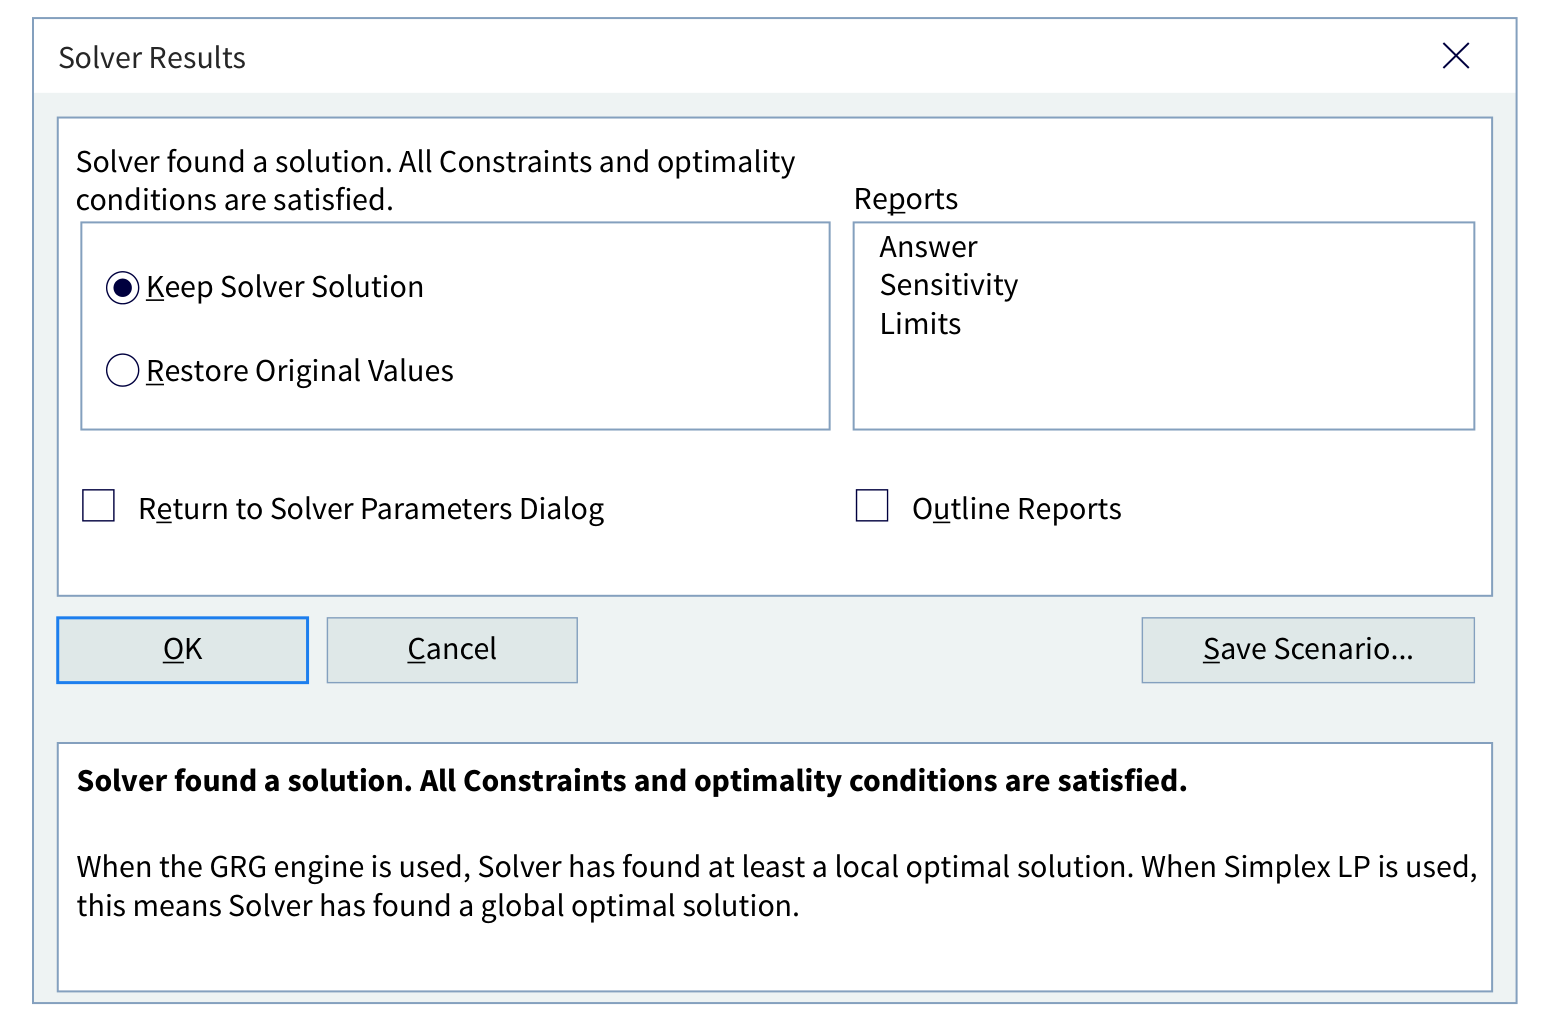
\includegraphics[width=0.95\textwidth,height=0.75\textheight,keepaspectratio]{../textbookForPractice/Figures/Ch_03/ILLUSTRATION 3.27.png}
    \end{figure}
\end{frame}

\begin{frame}{ILLUSTRATION 3.27\_1}

    \begin{figure}[h]
        \centering
        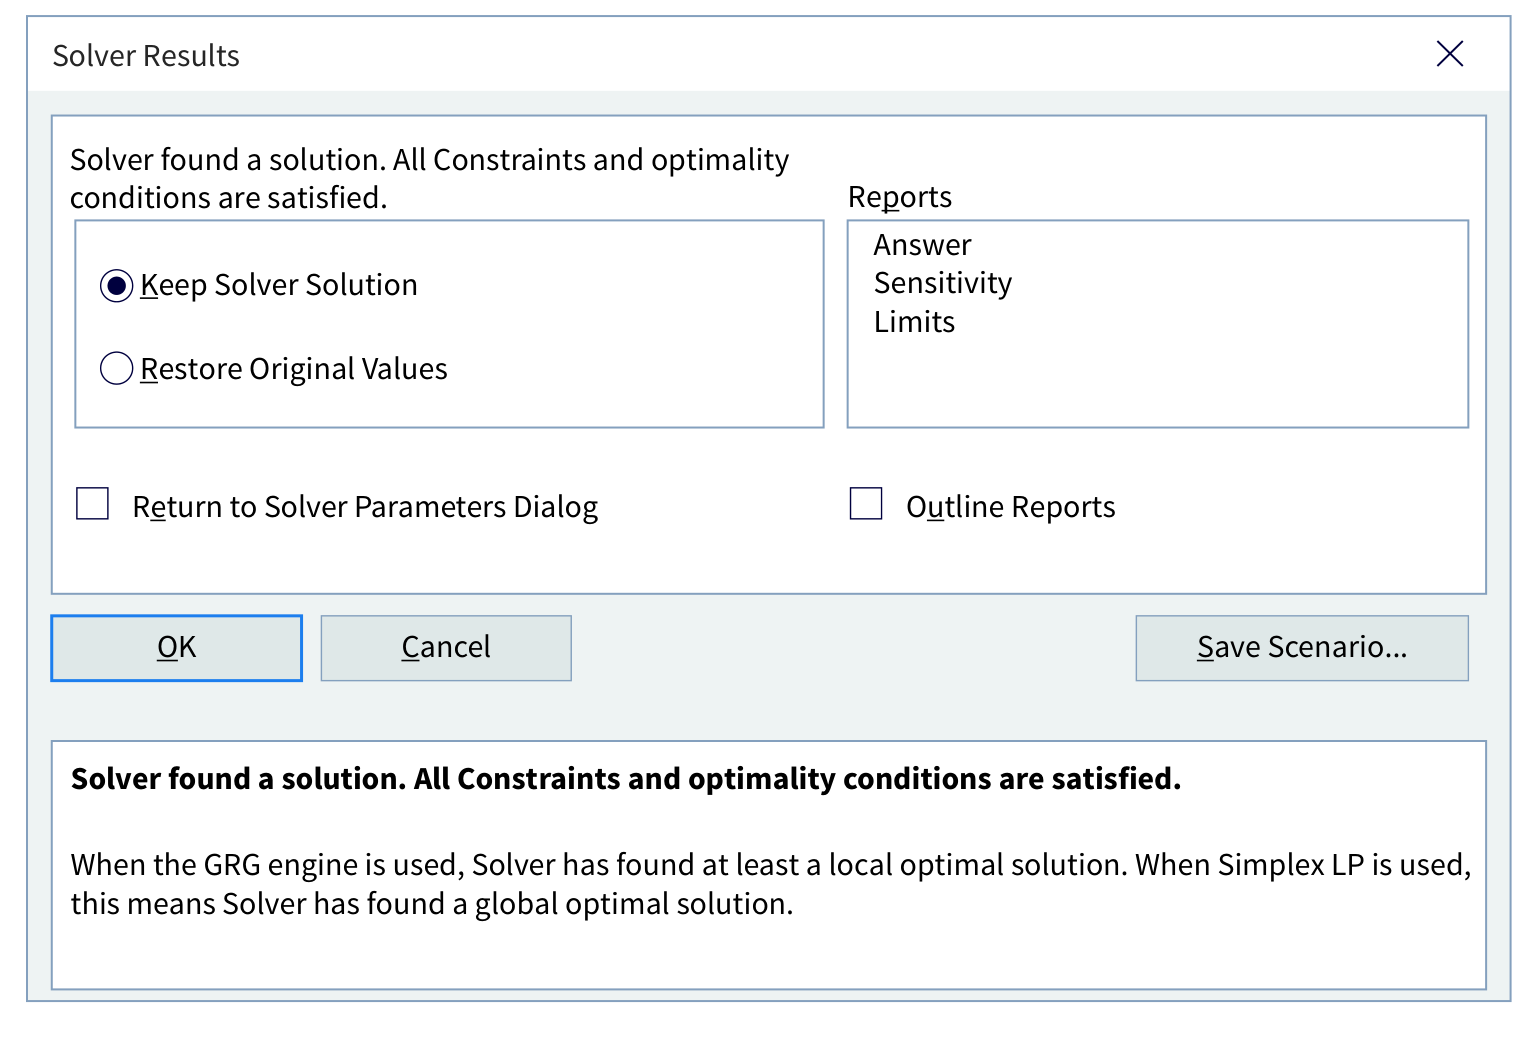
\includegraphics[width=0.95\textwidth,height=0.75\textheight,keepaspectratio]{../textbookForPractice/Figures/Ch_03/ILLUSTRATION 3.27_1.png}
    \end{figure}
\end{frame}

\begin{frame}{ILLUSTRATION 3.28}

    \begin{figure}[h]
        \centering
        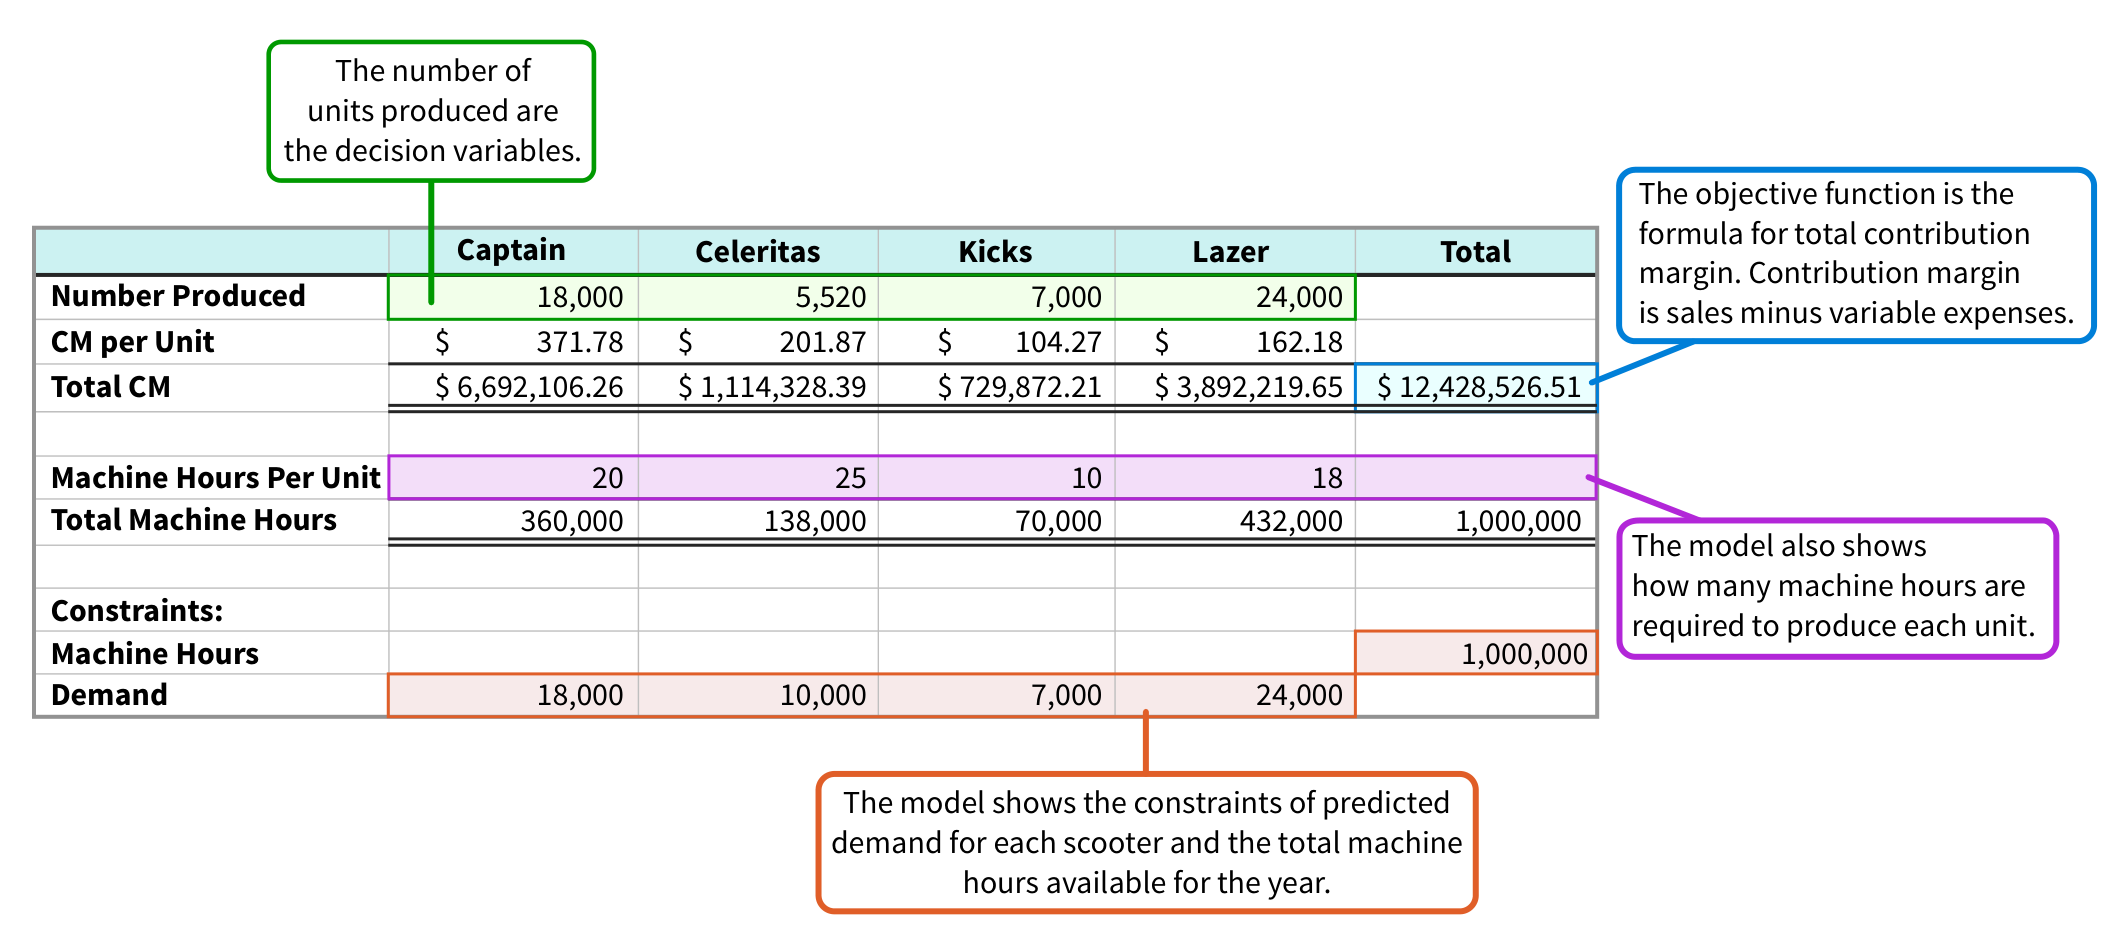
\includegraphics[width=0.95\textwidth,height=0.75\textheight,keepaspectratio]{../textbookForPractice/Figures/Ch_03/ILLUSTRATION 3.28.png}
    \end{figure}
\end{frame}

\begin{frame}{ILLUSTRATION 3.28\_1}

    \begin{figure}[h]
        \centering
        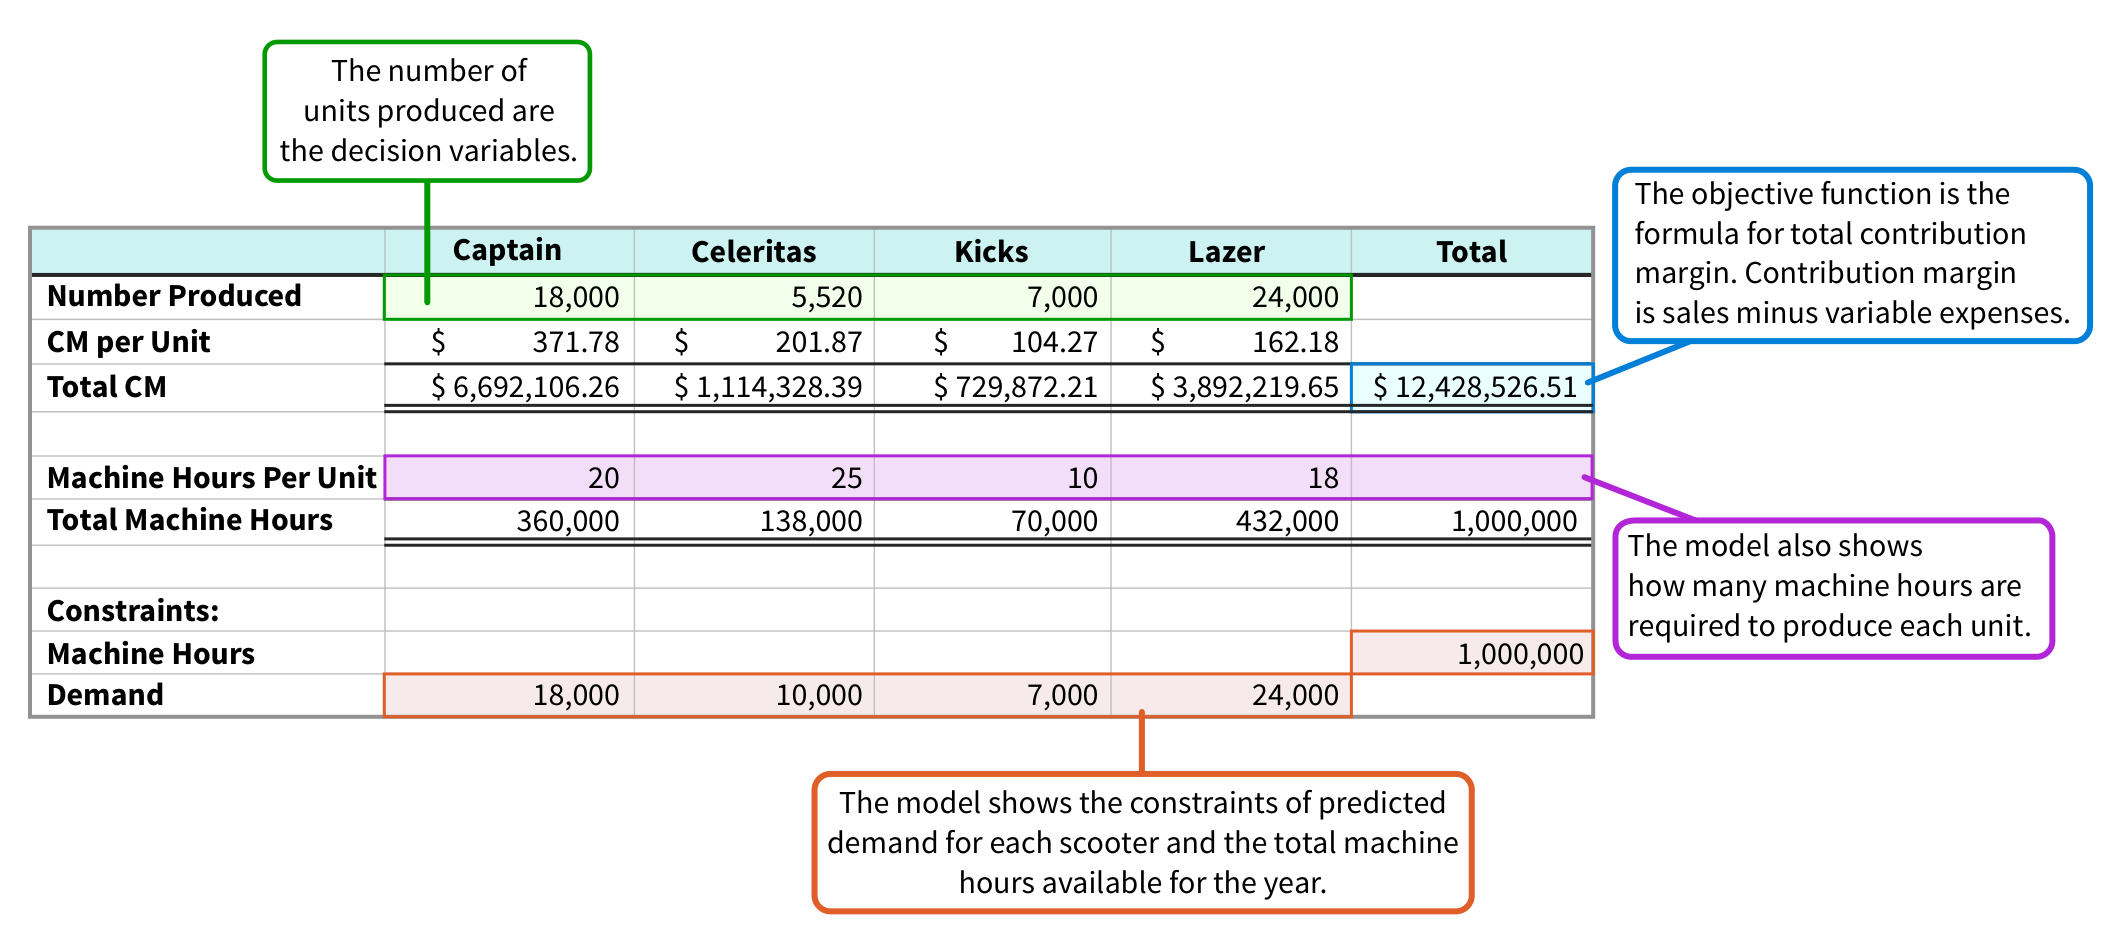
\includegraphics[width=0.95\textwidth,height=0.75\textheight,keepaspectratio]{../textbookForPractice/Figures/Ch_03/ILLUSTRATION 3.28_1.png}
    \end{figure}
\end{frame}

\begin{frame}{ILLUSTRATION 3.29}

    \begin{figure}[h]
        \centering
        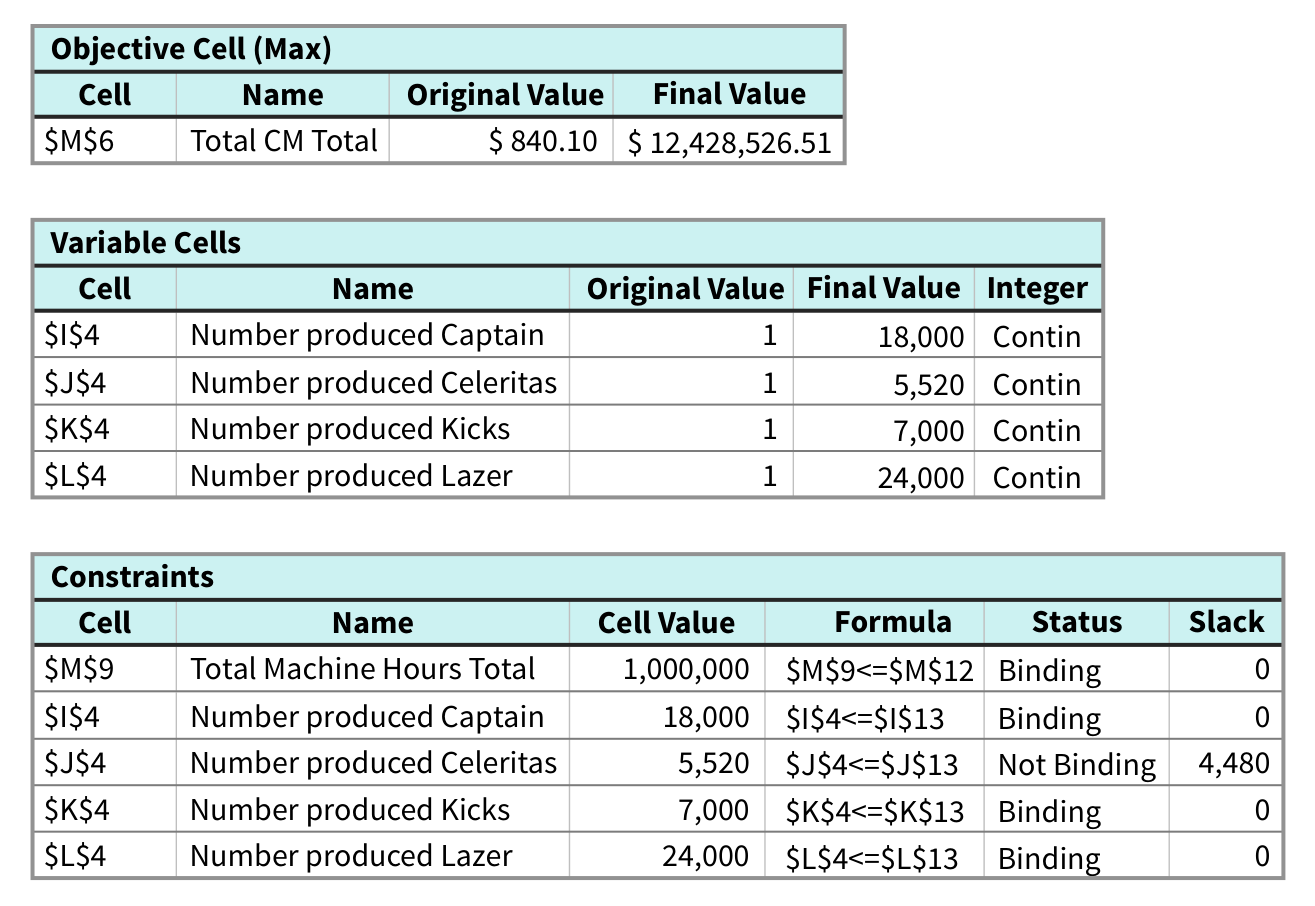
\includegraphics[width=0.95\textwidth,height=0.75\textheight,keepaspectratio]{../textbookForPractice/Figures/Ch_03/ILLUSTRATION 3.29.png}
    \end{figure}
\end{frame}

\begin{frame}{ILLUSTRATION 3.30}

    \begin{figure}[h]
        \centering
        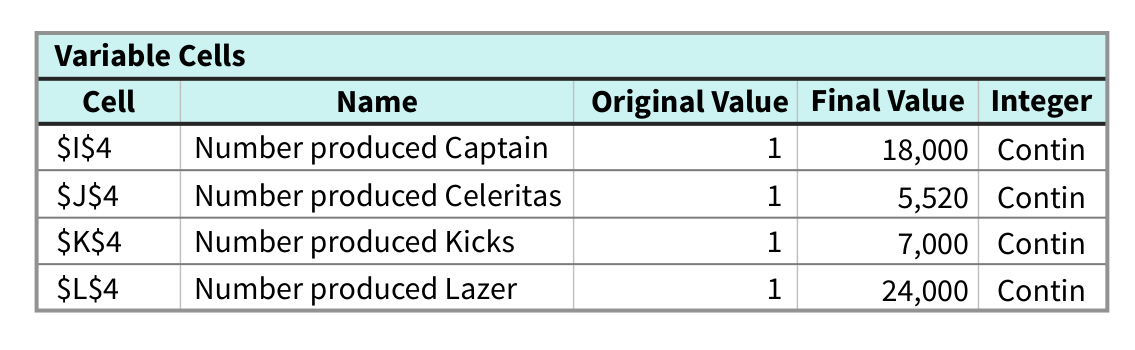
\includegraphics[width=0.95\textwidth,height=0.75\textheight,keepaspectratio]{../textbookForPractice/Figures/Ch_03/ILLUSTRATION 3.30.png}
    \end{figure}
\end{frame}

\begin{frame}{ILLUSTRATION 3.31}

    \begin{figure}[h]
        \centering
        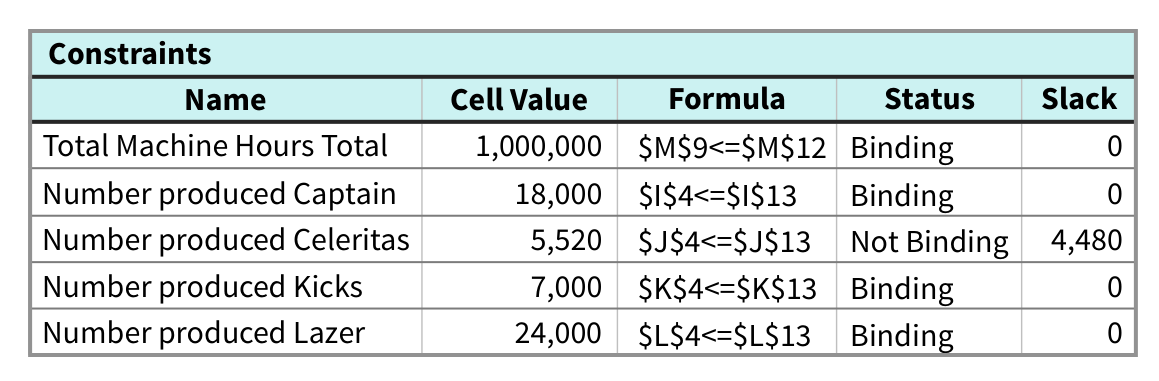
\includegraphics[width=0.95\textwidth,height=0.75\textheight,keepaspectratio]{../textbookForPractice/Figures/Ch_03/ILLUSTRATION 3.31.png}
    \end{figure}
\end{frame}

\begin{frame}{ILLUSTRATION 3.32}

    \begin{figure}[h]
        \centering
        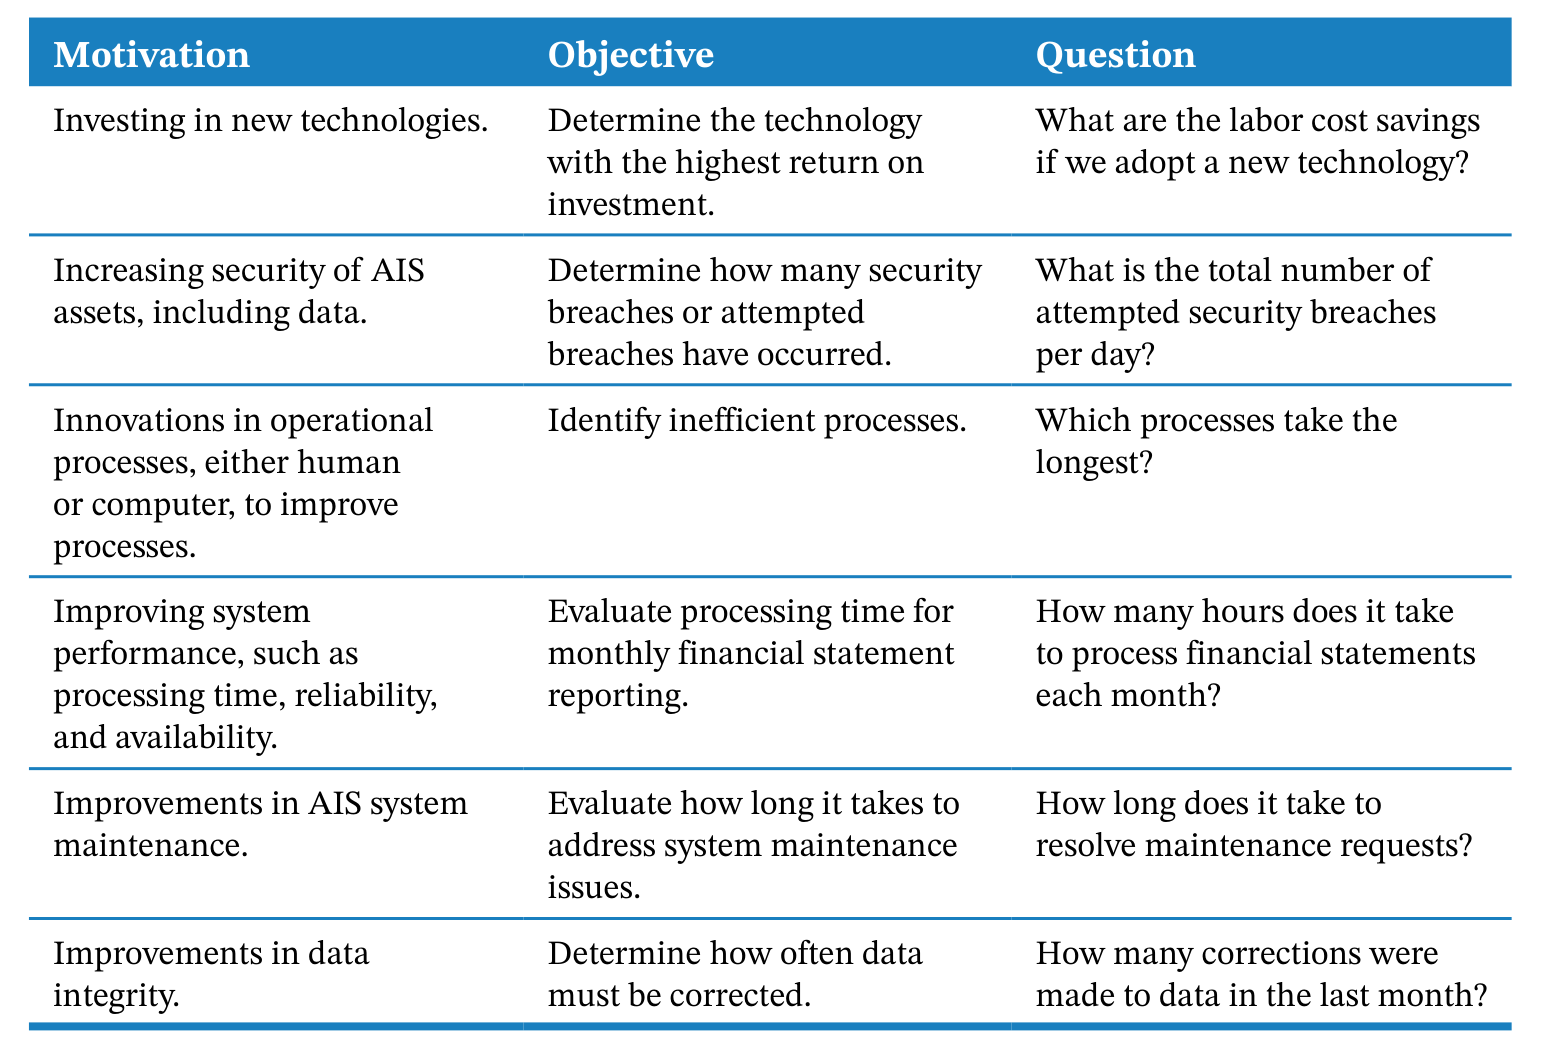
\includegraphics[width=0.95\textwidth,height=0.75\textheight,keepaspectratio]{../textbookForPractice/Figures/Ch_03/ILLUSTRATION 3.32.png}
    \end{figure}
\end{frame}

\begin{frame}{ILLUSTRATION 3.33}

    \begin{figure}[h]
        \centering
        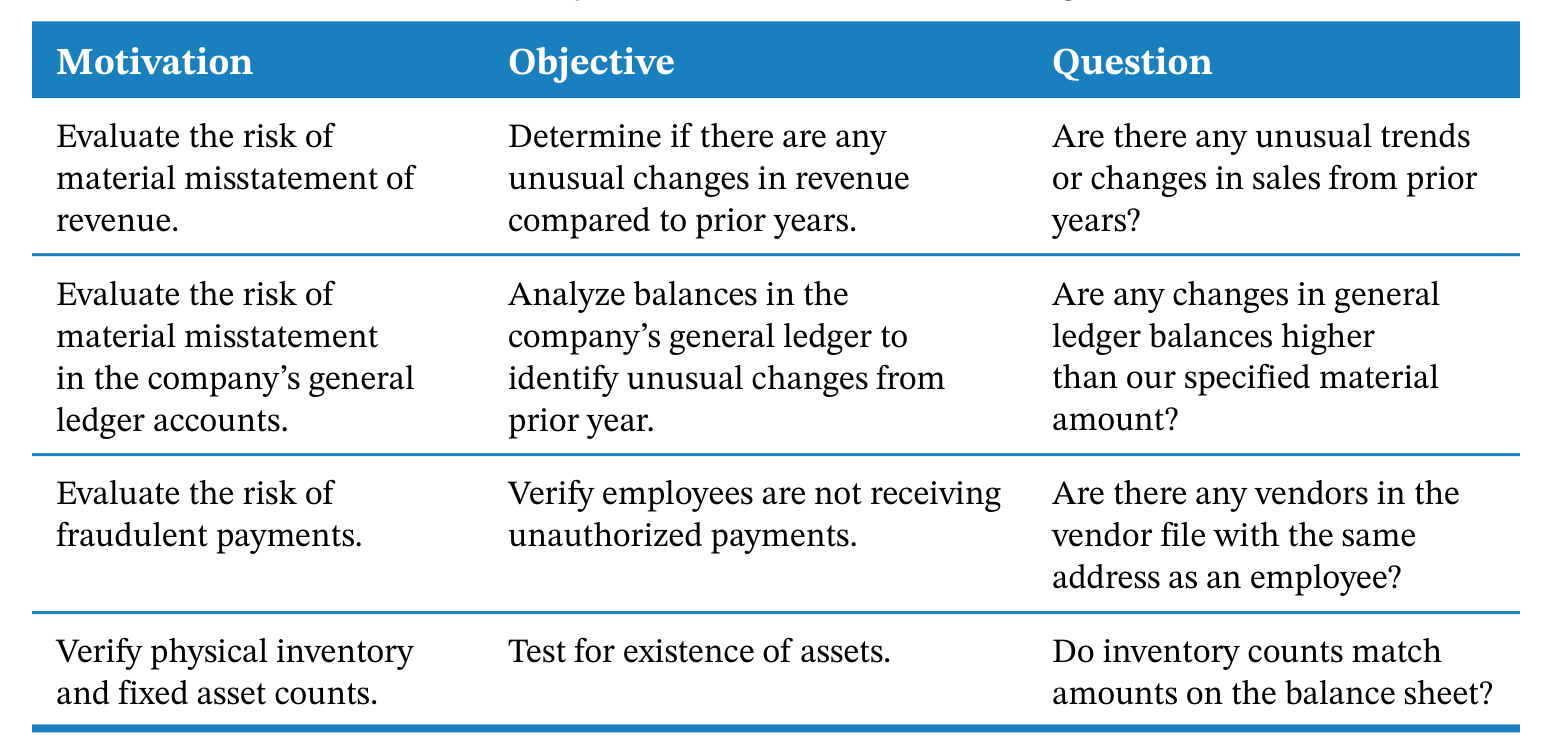
\includegraphics[width=0.95\textwidth,height=0.75\textheight,keepaspectratio]{../textbookForPractice/Figures/Ch_03/ILLUSTRATION 3.33.png}
    \end{figure}
\end{frame}

\begin{frame}{Apply It 3.4}

    \begin{figure}[h]
        \centering
        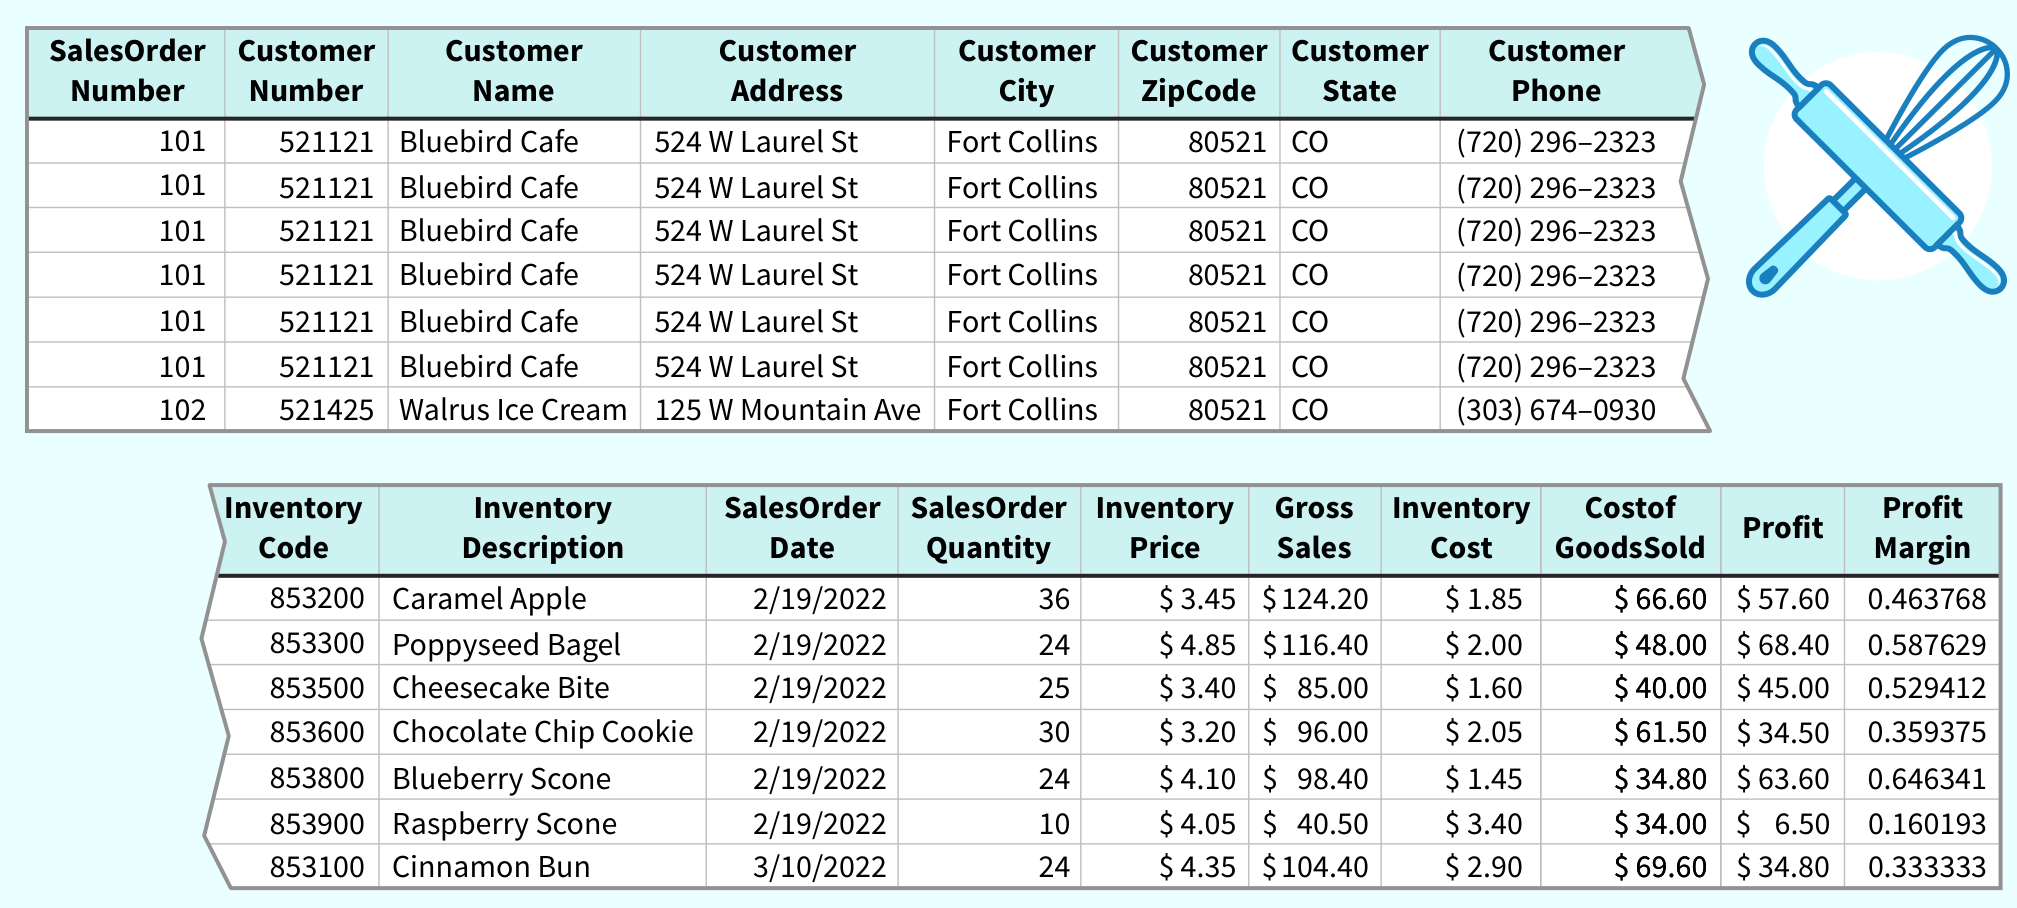
\includegraphics[width=0.95\textwidth,height=0.75\textheight,keepaspectratio]{../textbookForPractice/Figures/Ch_03/Apply It 3.4.png}
    \end{figure}
\end{frame}

\begin{frame}{3.5 Làm thế nào để phát triển Câu hỏi Đề xuất?}
\begin{itemize}
    \item \textbf{Câu hỏi Đề xuất (Prescriptive Questions):} Là đỉnh cao của phân tích dữ liệu trưởng thành. Nó cung cấp lời khuyên hoặc gợi ý hành động tự động.
    \item \textbf{Trọng tâm cốt lõi:} Tìm câu trả lời cho câu hỏi \textbf{"Chúng ta nên làm gì?"} (What should we do?).
    \item \textbf{Vai trò:} Không chỉ dự đoán điều gì sẽ xảy ra mà còn đưa ra giải pháp tối ưu nhất nhằm tối đa hóa lợi ích hoặc tối thiểu hóa rủi ro cho doanh nghiệp.
\end{itemize}
\end{frame}

\begin{frame}{Đặc điểm của Câu hỏi Đề xuất}
\begin{itemize}
    \item \textbf{Bản chất Tối ưu hóa:} Giải quyết các bài toán có nhiều ràng buộc (Constraints) tài nguyên như nguồn vốn, năng suất máy móc, nhân lực.
    \item \textbf{Hỗ trợ Trí tuệ Nhân tạo (AI):} Phân tích đề xuất sử dụng rất nhiều thuật toán tối ưu hóa, học máy và hệ chuyên gia để đưa ra các kịch bản hành động.
    \item \textbf{Mục đích cuối cùng:} Ra quyết định tự động hoặc hỗ trợ ra quyết định với mức độ tin cậy cực cao.
\end{itemize}
\end{frame}

\begin{frame}{Phân tích What-If và Tối ưu hóa}
\begin{itemize}
    \item \textbf{Phân tích What-If (Kịch bản):} Đánh giá kết quả của mục tiêu sẽ thay đổi như thế nào nếu chúng ta thay đổi một hoặc nhiều giả định đầu vào. (Ví dụ: Lợi nhuận sẽ ra sao nếu chi phí nguyên liệu tăng 10\%?).
    \item \textbf{Tối ưu hóa (Optimization):} Tìm kiếm điểm "Cực trị" (Tối đa hóa hoặc Tối thiểu hóa) dựa trên hàm mục tiêu và các ràng buộc. Thuật toán quy hoạch tuyến tính (Linear Programming) là một công cụ phổ biến.
\end{itemize}
\end{frame}

\begin{frame}{Ví dụ Phân tích Đề xuất (Kế toán Quản trị)}
\begin{itemize}
    \item \textbf{Bối cảnh:} Công ty sản xuất 3 loại sản phẩm khác nhau trên cùng một dây chuyền, nhưng tổng số giờ máy chạy tối đa trong tháng bị giới hạn ở mức 10,000 giờ.
    \item \textbf{Câu hỏi Đề xuất:} "Phối thức bán hàng (Sales Mix) tối ưu nào sẽ mang lại tổng lợi nhuận cao nhất cho công ty trong điều kiện hạn chế về giờ máy?".
    \item \textbf{Hành động:} Thiết lập mô hình toán học sử dụng Excel Solver để tìm ra chính xác số lượng từng sản phẩm cần sản xuất.
\end{itemize}
\end{frame}

\begin{frame}{Giải quyết bài toán ràng buộc nguồn lực}
\begin{itemize}
    \item \textbf{Xác định Hàm Mục tiêu (Objective Function):} Thường là Tối đa hóa Lợi nhuận gộp, Tối đa hóa Dòng tiền, hoặc Tối thiểu hóa Chi phí.
    \item \textbf{Xác định Biến quyết định (Decision Variables):} Số lượng sản phẩm sản xuất, Mức giá bán, Khối lượng nguyên liệu mua...
    \item \textbf{Xác định Ràng buộc (Constraints):} Hạn mức tín dụng, Công suất máy, Nhu cầu thị trường, Giới hạn ngân sách.
\end{itemize}
\end{frame}

\begin{frame}{Trực quan hóa kết quả phân tích Đề xuất}
\begin{itemize}
    \item \textbf{Biểu đồ Độ nhạy (Tornado Charts):} Rất hiệu quả để thể hiện các biến số nào có tác động lớn nhất đến kết quả mục tiêu.
    \item \textbf{Bảng dữ liệu Kịch bản (Scenario Data Tables):} So sánh song song các chỉ số tài chính giữa các Kịch bản Tốt nhất, Xấu nhất, và Khả năng cao nhất.
\end{itemize}
\end{frame}

\begin{frame}{ILLUSTRATION 3.34}

    \begin{figure}[h]
        \centering
        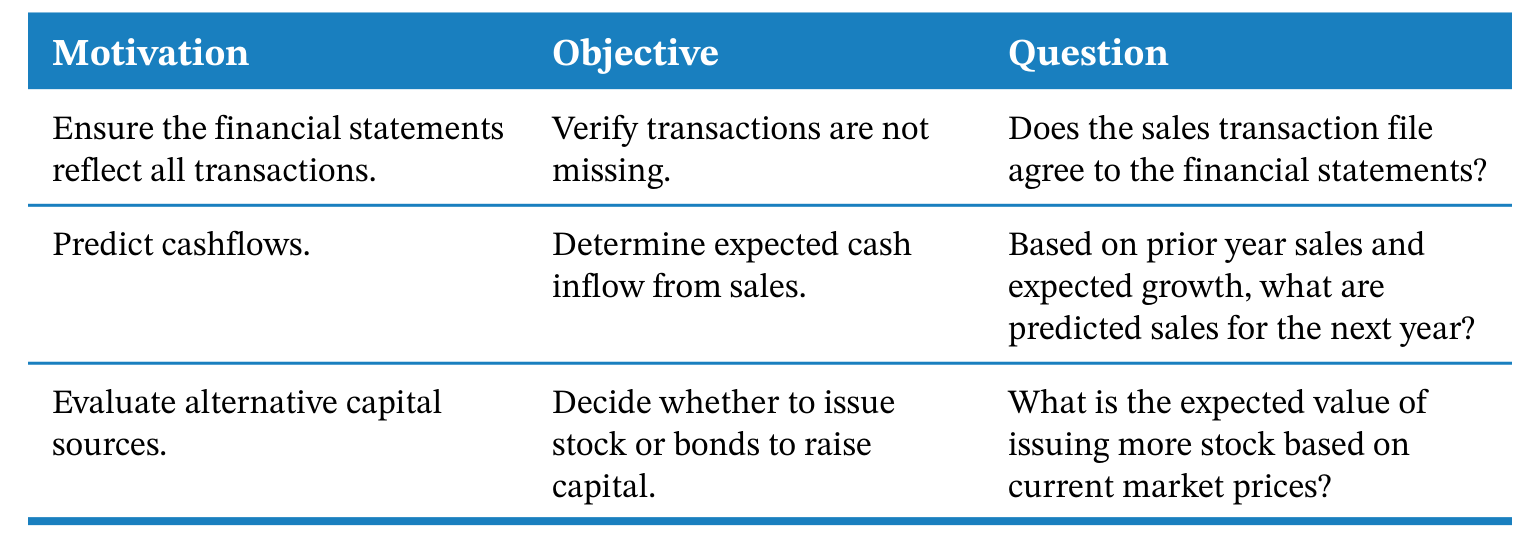
\includegraphics[width=0.95\textwidth,height=0.75\textheight,keepaspectratio]{../textbookForPractice/Figures/Ch_03/ILLUSTRATION 3.34.png}
    \end{figure}
\end{frame}

\begin{frame}{ILLUSTRATION 3.35}

    \begin{figure}[h]
        \centering
        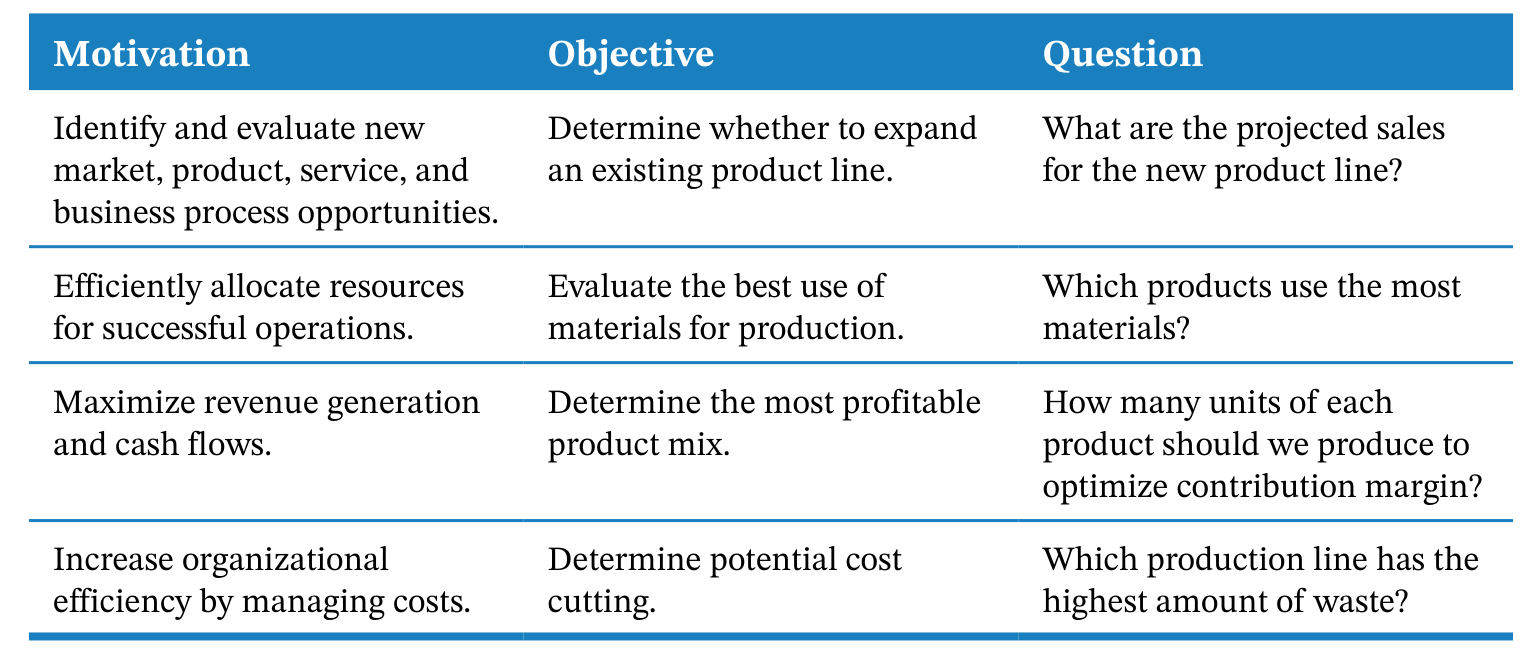
\includegraphics[width=0.95\textwidth,height=0.75\textheight,keepaspectratio]{../textbookForPractice/Figures/Ch_03/ILLUSTRATION 3.35.png}
    \end{figure}
\end{frame}

\begin{frame}{ILLUSTRATION 3.36}

    \begin{figure}[h]
        \centering
        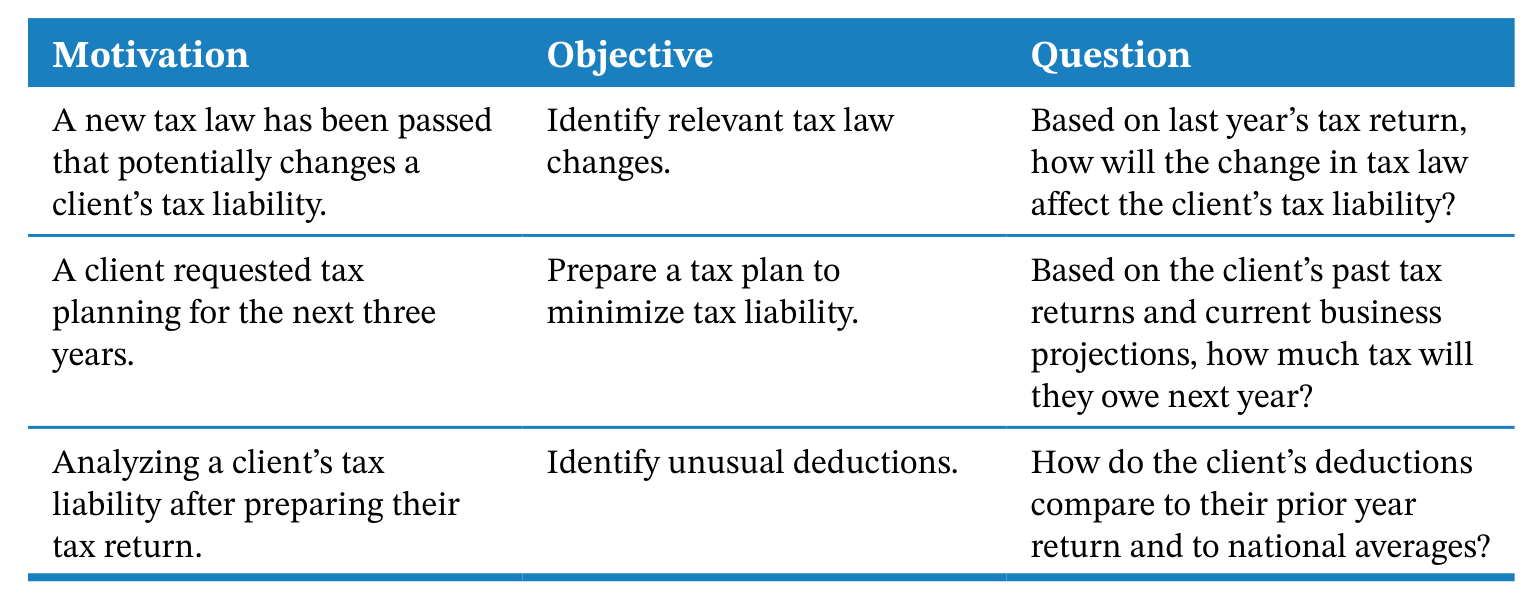
\includegraphics[width=0.95\textwidth,height=0.75\textheight,keepaspectratio]{../textbookForPractice/Figures/Ch_03/ILLUSTRATION 3.36.png}
    \end{figure}
\end{frame}

\begin{frame}{ILLUSTRATION 3.37}

    \begin{figure}[h]
        \centering
        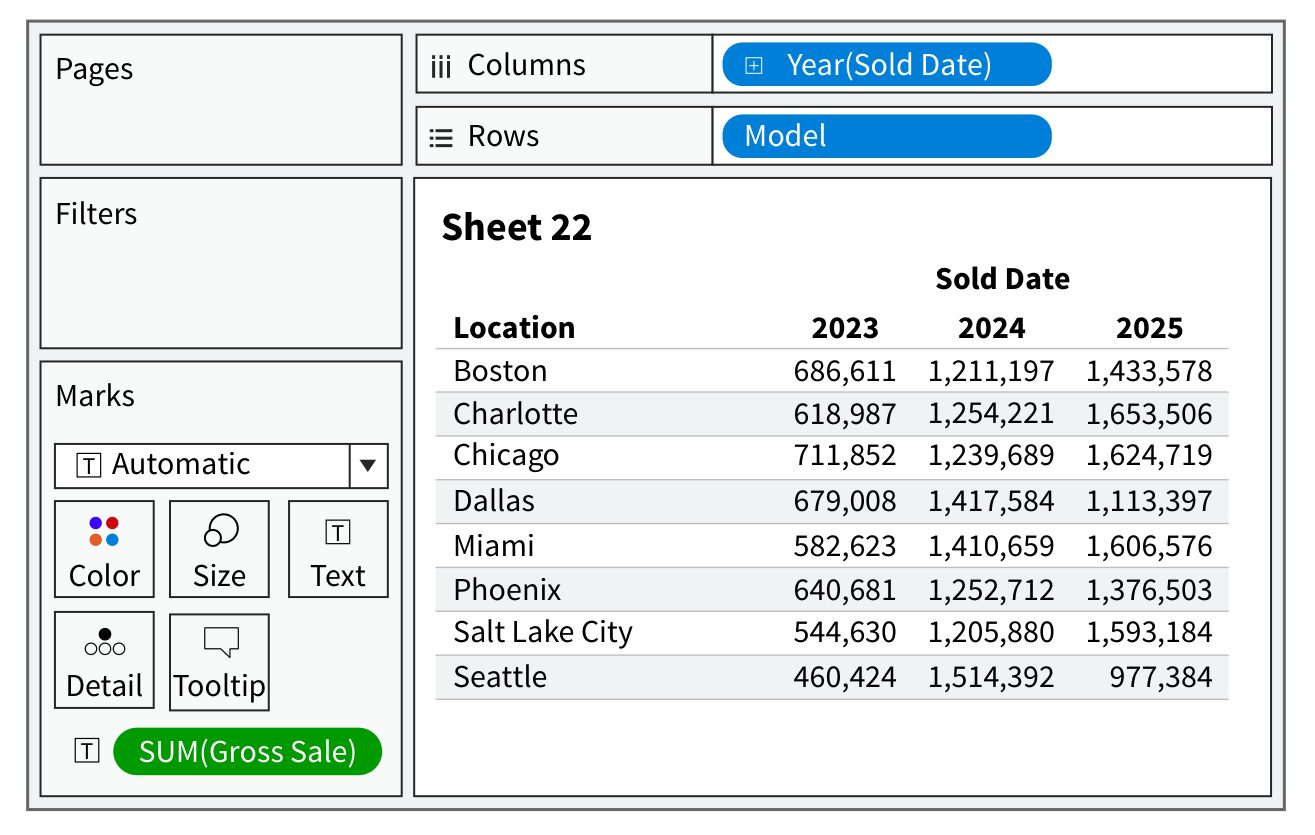
\includegraphics[width=0.95\textwidth,height=0.75\textheight,keepaspectratio]{../textbookForPractice/Figures/Ch_03/ILLUSTRATION 3.37.png}
    \end{figure}
\end{frame}

\begin{frame}{ILLUSTRATION 3.37\_1}

    \begin{figure}[h]
        \centering
        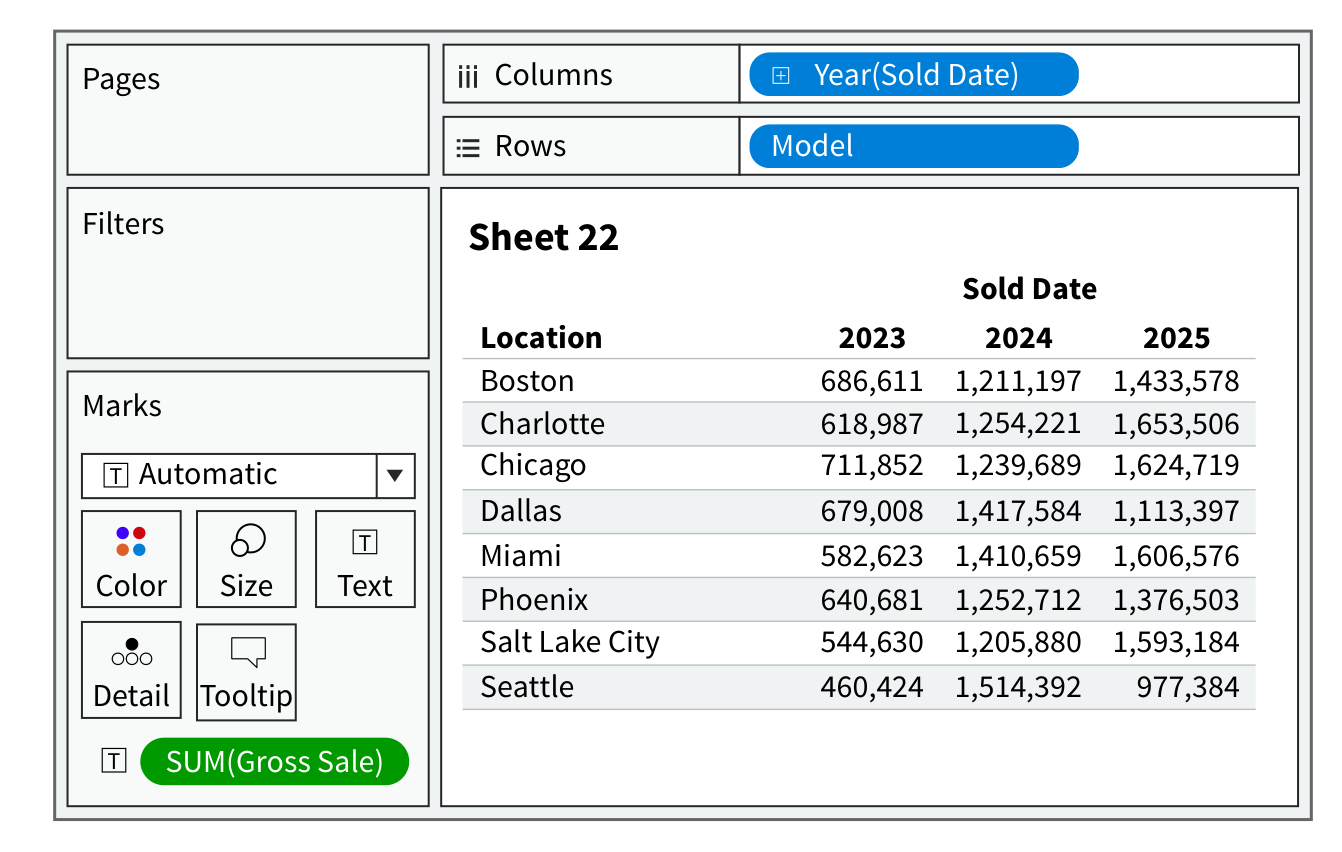
\includegraphics[width=0.95\textwidth,height=0.75\textheight,keepaspectratio]{../textbookForPractice/Figures/Ch_03/ILLUSTRATION 3.37_1.png}
    \end{figure}
\end{frame}

\begin{frame}{ILLUSTRATION 3.38}

    \begin{figure}[h]
        \centering
        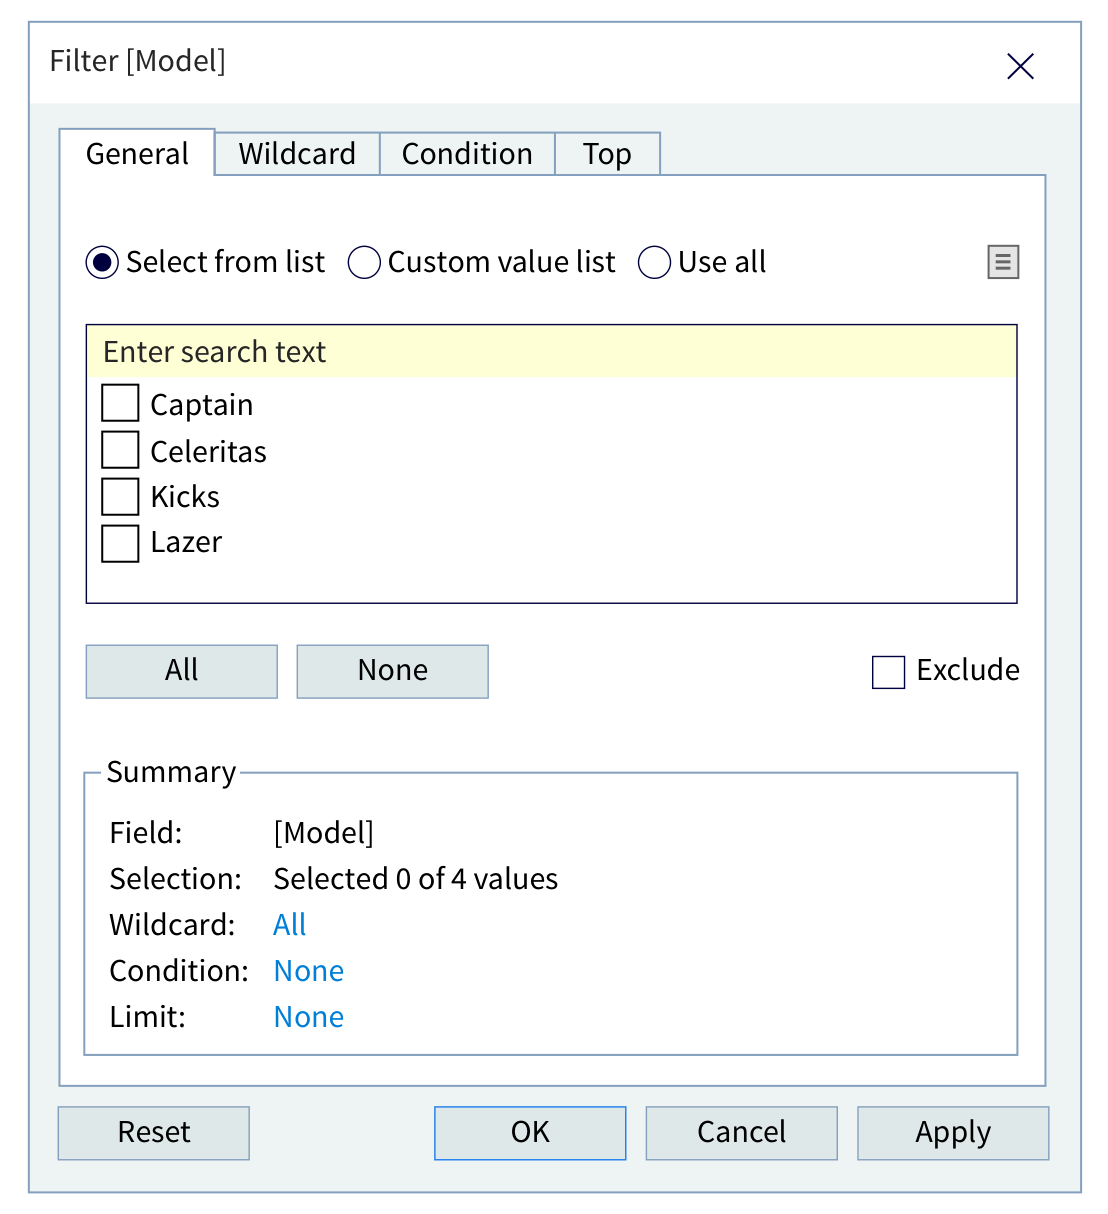
\includegraphics[width=0.95\textwidth,height=0.75\textheight,keepaspectratio]{../textbookForPractice/Figures/Ch_03/ILLUSTRATION 3.38.png}
    \end{figure}
\end{frame}

\begin{frame}{ILLUSTRATION 3.38\_1}

    \begin{figure}[h]
        \centering
        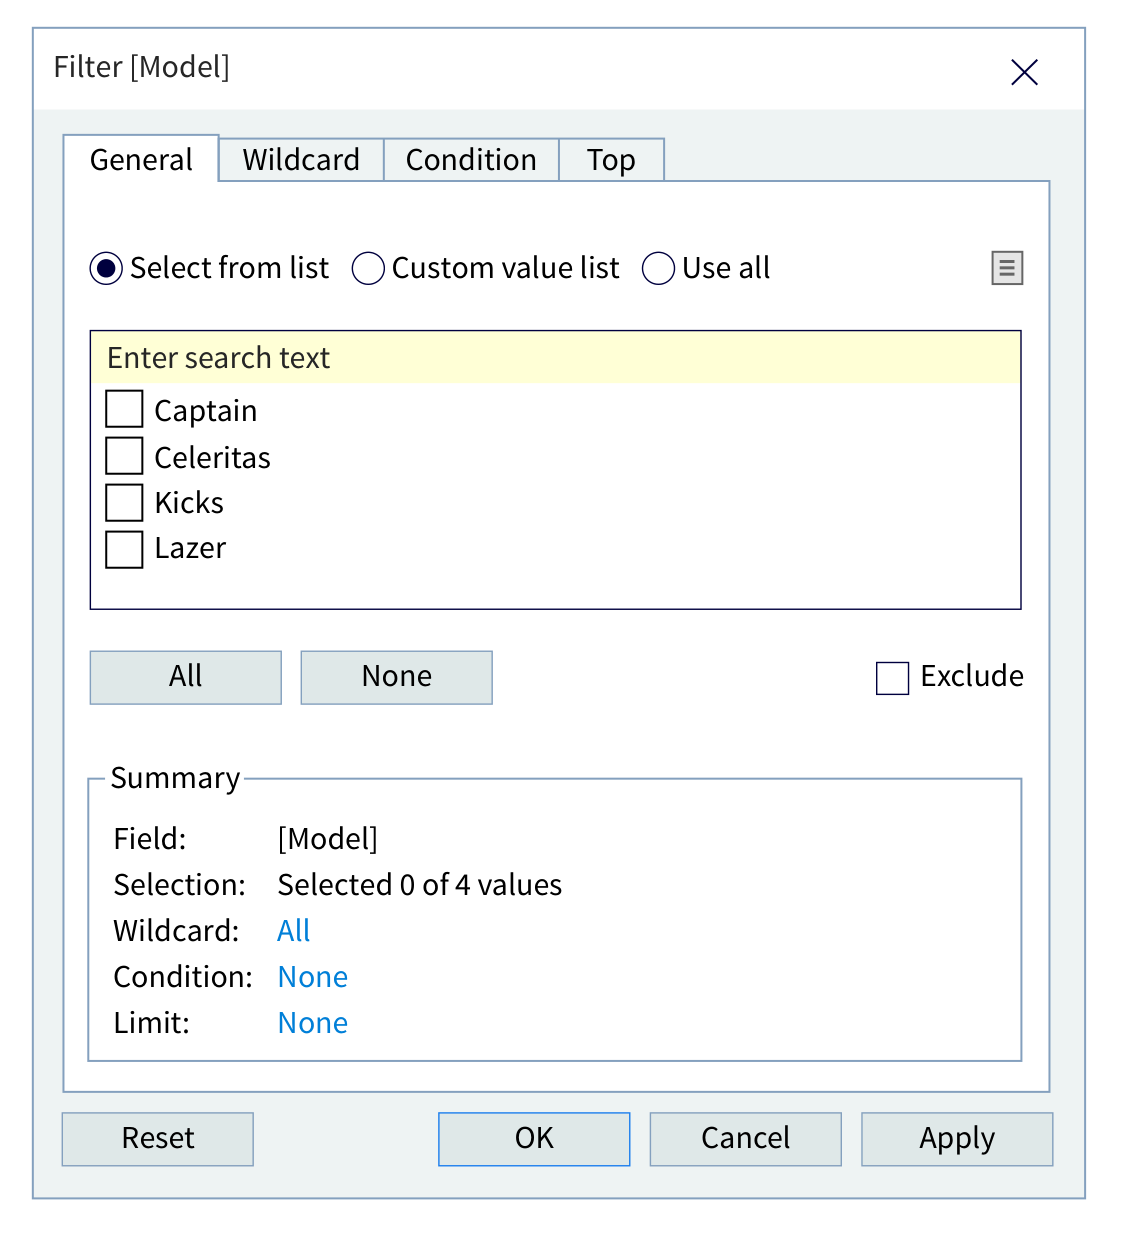
\includegraphics[width=0.95\textwidth,height=0.75\textheight,keepaspectratio]{../textbookForPractice/Figures/Ch_03/ILLUSTRATION 3.38_1.png}
    \end{figure}
\end{frame}

\begin{frame}{ILLUSTRATION 3.39}

    \begin{figure}[h]
        \centering
        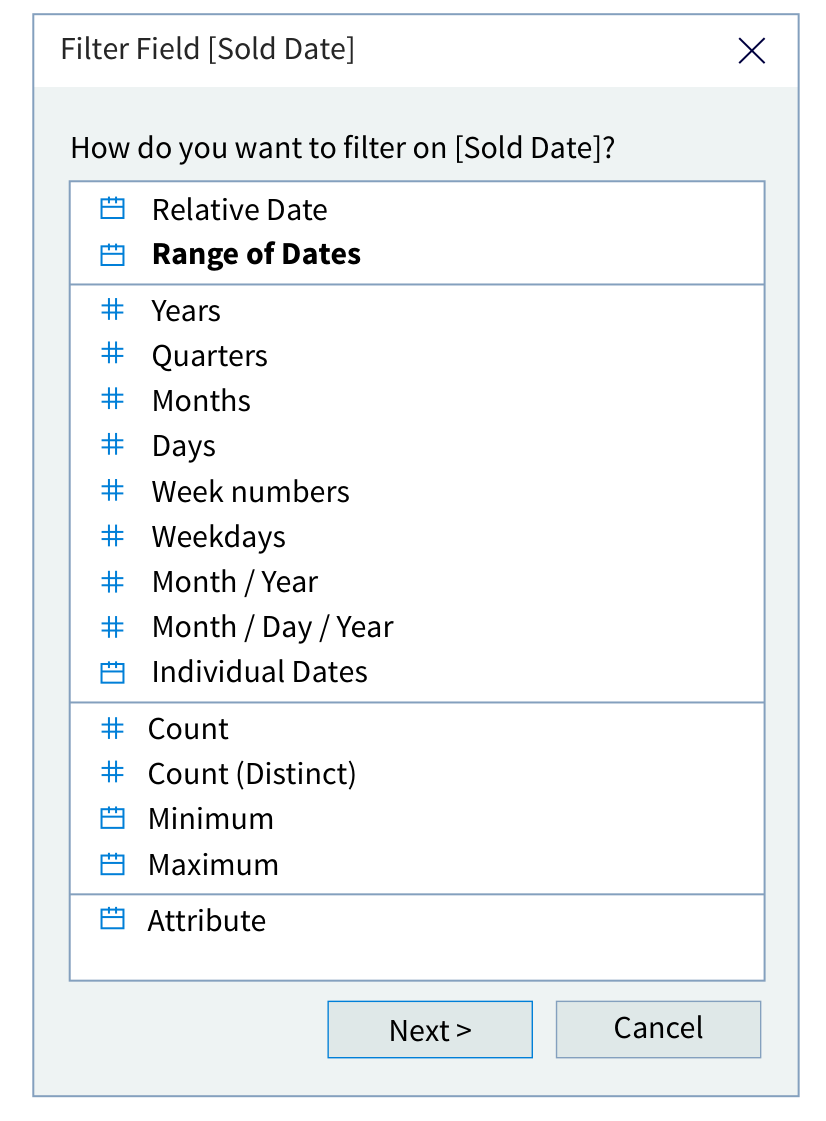
\includegraphics[width=0.95\textwidth,height=0.75\textheight,keepaspectratio]{../textbookForPractice/Figures/Ch_03/ILLUSTRATION 3.39.png}
    \end{figure}
\end{frame}

\begin{frame}{ILLUSTRATION 3.40}

    \begin{figure}[h]
        \centering
        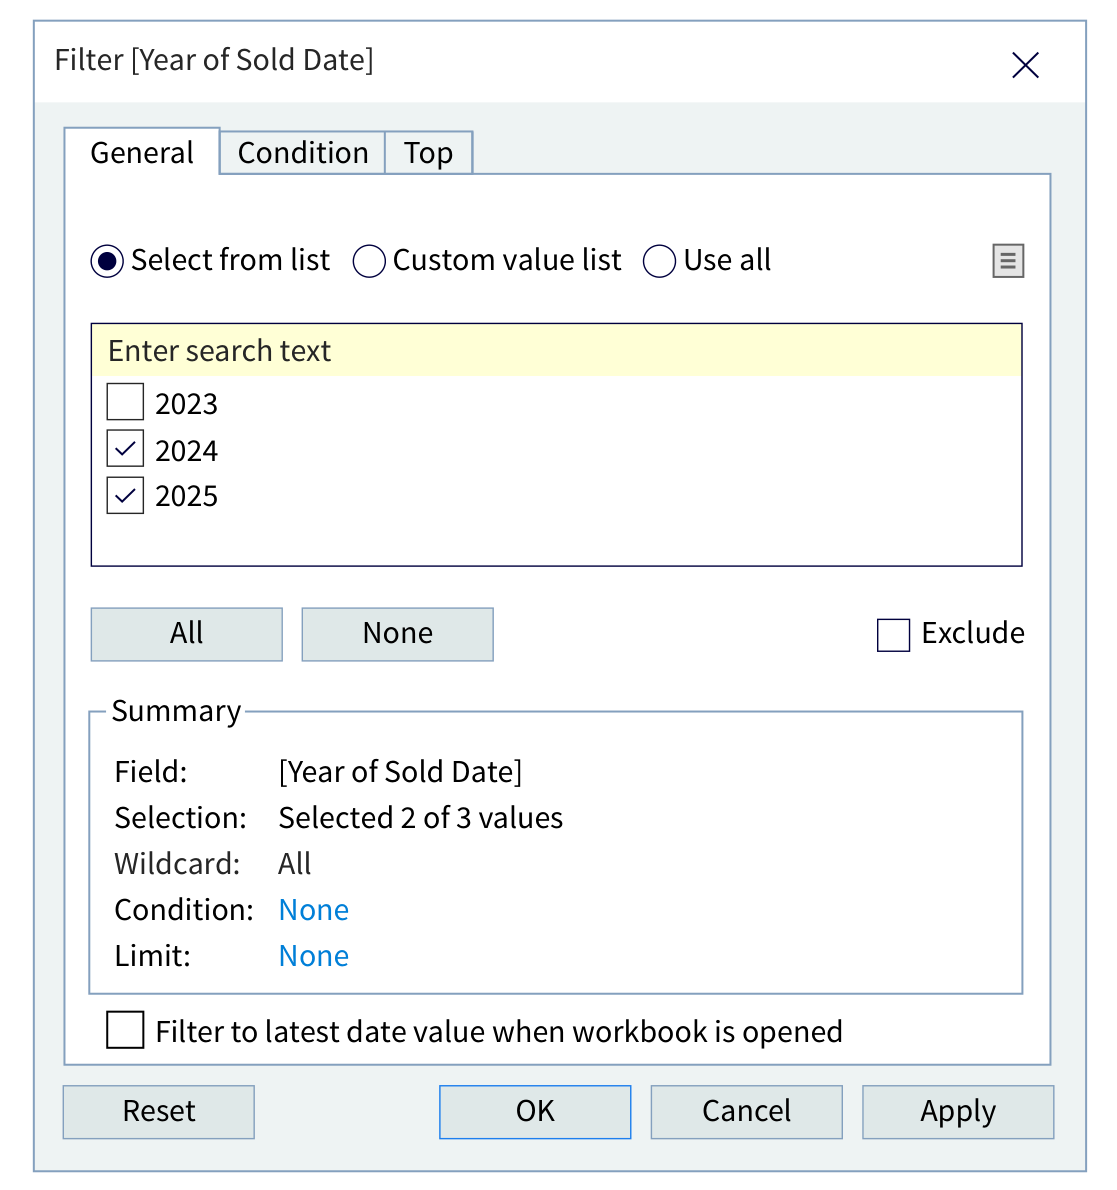
\includegraphics[width=0.95\textwidth,height=0.75\textheight,keepaspectratio]{../textbookForPractice/Figures/Ch_03/ILLUSTRATION 3.40.png}
    \end{figure}
\end{frame}

\begin{frame}{3.6 Ứng dụng trong Thực tiễn Nghề nghiệp}
\begin{itemize}
    \item \textbf{Sự giao thoa (Intersection):} Việc đặt câu hỏi phân tích không tách rời khỏi lĩnh vực chuyên môn của kế toán. Mỗi lĩnh vực có những đặc thù riêng biệt.
    \item \textbf{Tư duy tích hợp:} Kế toán viên thời kỳ 4.0 cần kết hợp giữa năng lực chuyên môn nghiệp vụ (Domain Knowledge) với các kỹ năng phân tích dữ liệu hiện đại (Analytics Skills).
    \item Các slide tiếp theo sẽ phân tích sâu việc ứng dụng câu hỏi phân tích vào 4 trụ cột của ngành: AIS, Kiểm toán, Kế toán Tài chính và Kế toán Quản trị.
\end{itemize}
\end{frame}

\begin{frame}{Hệ thống Thông tin Kế toán (AIS)}
\begin{itemize}
    \item \textbf{Động lực:} Đảm bảo hệ thống hoạt động hiệu quả, an toàn và toàn vẹn dữ liệu.
    \item \textbf{Mô tả:} Có bao nhiêu người dùng có quyền admin trong hệ thống ERP?
    \item \textbf{Chẩn đoán:} Tại sao thời gian xử lý một lệnh thanh toán lại tăng gấp đôi trong tháng qua?
    \item \textbf{Dự đoán:} Hệ thống máy chủ có nguy cơ bị quá tải vào dịp quyết toán cuối năm hay không?
    \item \textbf{Đề xuất:} Cần nâng cấp những module nào để tối ưu hóa quy trình luân chuyển chứng từ?
\end{itemize}
\end{frame}

\begin{frame}{Kiểm toán (Auditing)}
\begin{itemize}
    \item \textbf{Động lực:} Thu thập bằng chứng kiểm toán đầy đủ, phù hợp để đánh giá rủi ro và xác nhận BCTC.
    \item \textbf{Mô tả:} Tổng giá trị các bút toán điều chỉnh vào ngày 31/12 là bao nhiêu?
    \item \textbf{Chẩn đoán:} Tại sao tài khoản chi phí quản lý doanh nghiệp lại phát sinh một số lượng lớn các hóa đơn dưới hạn mức phê duyệt? (Chia nhỏ hóa đơn để trốn duyệt).
    \item \textbf{Dự đoán:} Khả năng doanh nghiệp không đáp ứng được giả định hoạt động liên tục (Going concern) trong 12 tháng tới là bao nhiêu?
    \item \textbf{Đề xuất:} Nên thiết kế các thủ tục kiểm toán bổ sung nào để đối phó với rủi ro có gian lận ở khoản mục Hàng Tồn Kho?
\end{itemize}
\end{frame}

\begin{frame}{Kế toán Tài chính (Financial Accounting)}
\begin{itemize}
    \item \textbf{Động lực:} Lập báo cáo tài chính chính xác, tuân thủ chuẩn mực và công bố thông tin minh bạch cho cổ đông.
    \item \textbf{Mô tả:} Lợi nhuận cơ bản trên cổ phiếu (EPS) của công ty trong quý này là bao nhiêu?
    \item \textbf{Chẩn đoán:} Tại sao dòng tiền thuần từ hoạt động kinh doanh lại âm trong khi lợi nhuận kế toán lại dương?
    \item \textbf{Dự đoán:} Doanh thu thuần dự kiến trong quý tiếp theo dựa trên backlog hợp đồng hiện tại là bao nhiêu?
    \item \textbf{Đề xuất:} Doanh nghiệp có nên áp dụng chính sách vốn hóa chi phí lãi vay cho dự án mới để cải thiện tỷ suất sinh lời trên tài sản (ROA) trong ngắn hạn không?
\end{itemize}
\end{frame}

\begin{frame}{Kế toán Quản trị (Managerial Accounting)}
\begin{itemize}
    \item \textbf{Động lực:} Cung cấp thông tin ra quyết định nội bộ để cải thiện hiệu quả và kiểm soát chi phí.
    \item \textbf{Mô tả:} Tỷ lệ biến phí trên doanh thu của dòng sản phẩm X là bao nhiêu?
    \item \textbf{Chẩn đoán:} Tại sao biến động chi phí nguyên vật liệu trực tiếp (Materials Variance) lại không thuận lợi đáng kể ở phân xưởng 2?
    \item \textbf{Dự đoán:} Dựa trên biến động giá dầu thế giới, chi phí vận chuyển logistics của công ty sẽ tăng bao nhiêu \% trong năm tới?
    \item \textbf{Đề xuất:} Cần thay đổi nhà cung cấp hay cải tiến quy trình công nghệ để đạt được mục tiêu chi phí mục tiêu (Target Costing)?
\end{itemize}
\end{frame}

\begin{frame}{Kế toán Thuế (Tax Accounting)}
\begin{itemize}
    \item \textbf{Động lực:} Tuân thủ luật thuế, tối thiểu hóa nghĩa vụ thuế hợp pháp và tránh các rủi ro thanh tra.
    \item \textbf{Mô tả:} Thuế suất hữu hiệu (Effective Tax Rate) của tập đoàn hiện tại là bao nhiêu?
    \item \textbf{Chẩn đoán:} Tại sao số thuế TNDN hoãn lại phải trả lại tăng mạnh trong kỳ này? (Do chênh lệch tạm thời từ khấu hao tài sản).
    \item \textbf{Dự đoán:} Ước tính số thuế thu nhập doanh nghiệp phải nộp trong quý tới để lên kế hoạch dòng tiền nộp thuế.
    \item \textbf{Đề xuất:} Tập đoàn nên cấu trúc các giao dịch liên kết (Transfer Pricing) như thế nào để tối ưu hóa nghĩa vụ thuế toàn cầu nhưng vẫn tuân thủ nguyên tắc giá thị trường (Arm's length)?
\end{itemize}
\end{frame}

\begin{frame}{Ghép nối Động lực với các Lĩnh vực Chuyên môn}
\begin{itemize}
    \item \textbf{Mỗi bài toán - Một chiến lược:} Khi đối mặt với một vấn đề kế toán, việc phân loại đúng lĩnh vực chuyên môn (Thuế, Quản trị, Tài chính...) sẽ giúp xác định đúng cơ sở dữ liệu và hệ phương pháp phân tích.
    \item \textbf{Tư duy giải pháp toàn diện (Holistic Approach):} Một vấn đề thường yêu cầu phải đặt một chuỗi các câu hỏi từ Mô tả $\rightarrow$ Chẩn đoán $\rightarrow$ Dự đoán $\rightarrow$ Đề xuất.
\end{itemize}
\end{frame}

\begin{frame}{Tóm tắt Mục tiêu Học tập 1}
\begin{itemize}
    \item \textbf{LO 3.1:} Hiểu rõ tầm quan trọng của việc xác định động lực và mục tiêu trong phân tích dữ liệu, làm cơ sở định hình các câu hỏi phân tích.
    \item \textbf{LO 3.2:} Phát triển được các Câu hỏi Mô tả nhằm tóm tắt dữ liệu lịch sử ("Điều gì đã xảy ra?").
    \item \textbf{LO 3.3:} Đặt được các Câu hỏi Chẩn đoán nhằm tìm ra nguyên nhân của các vấn đề hoặc xu hướng ("Tại sao nó lại xảy ra?").
\end{itemize}
\end{frame}

\begin{frame}{Tóm tắt Mục tiêu Học tập 2}
\begin{itemize}
    \item \textbf{LO 3.4:} Xây dựng các Câu hỏi Dự đoán để dự báo xu hướng tương lai dựa trên dữ liệu quá khứ ("Điều gì sẽ xảy ra?").
    \item \textbf{LO 3.5:} Phát triển các Câu hỏi Đề xuất nhằm tối ưu hóa quyết định kinh doanh ("Chúng ta nên làm gì?").
    \item \textbf{LO 3.6:} Vận dụng các loại câu hỏi phân tích vào các lĩnh vực chuyên môn cụ thể của kế toán (Kiểm toán, Kế toán Quản trị, Kế toán Thuế...).
\end{itemize}
\end{frame}

\begin{frame}{ILLUSTRATION 3.41}

    \begin{figure}[h]
        \centering
        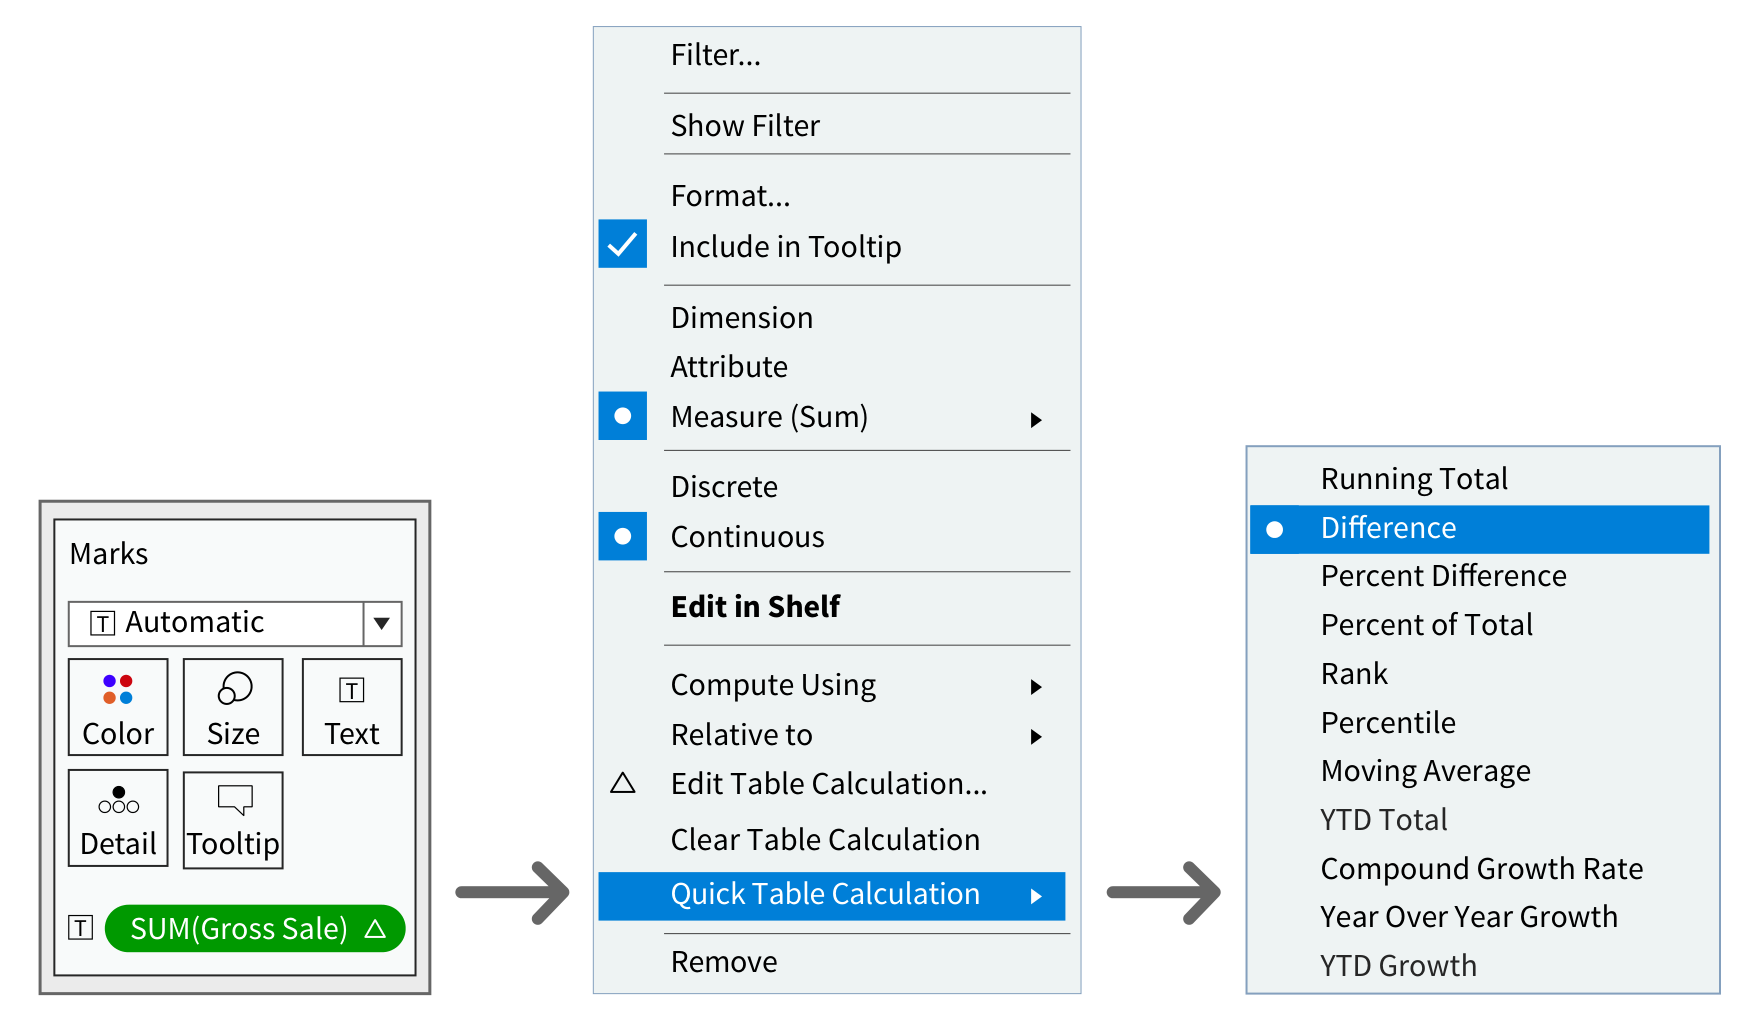
\includegraphics[width=0.95\textwidth,height=0.75\textheight,keepaspectratio]{../textbookForPractice/Figures/Ch_03/ILLUSTRATION 3.41.png}
    \end{figure}
\end{frame}

\begin{frame}{ILLUSTRATION 3.42}

    \begin{figure}[h]
        \centering
        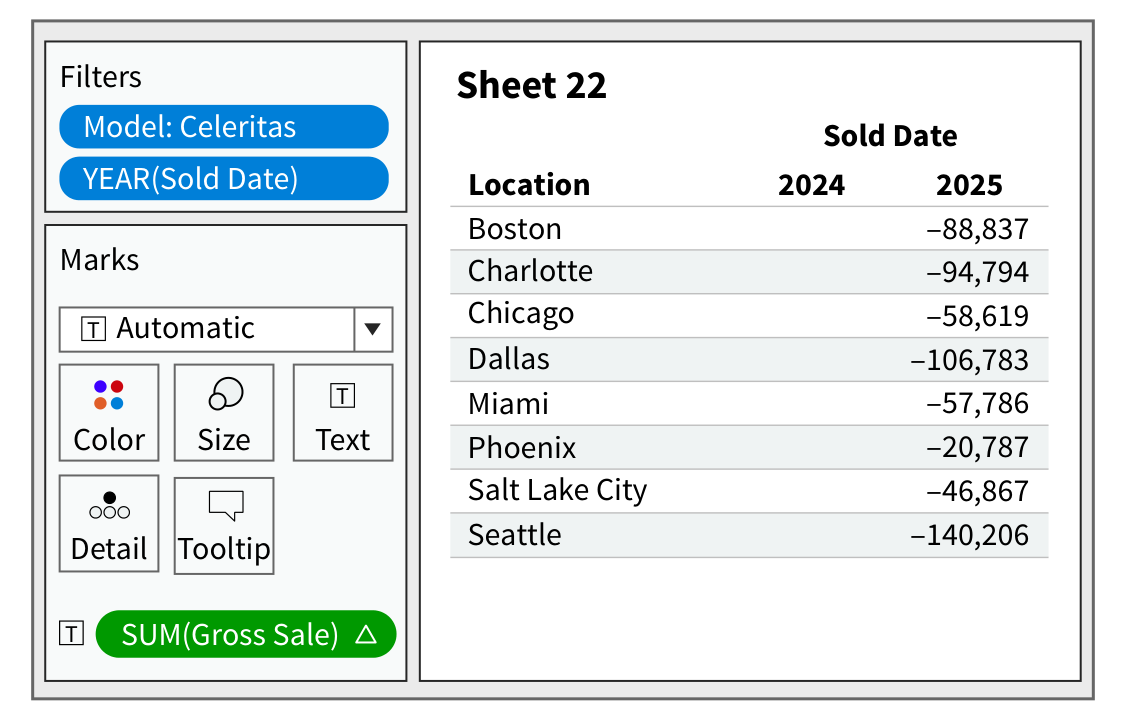
\includegraphics[width=0.95\textwidth,height=0.75\textheight,keepaspectratio]{../textbookForPractice/Figures/Ch_03/ILLUSTRATION 3.42.png}
    \end{figure}
\end{frame}

\begin{frame}{ILLUSTRATION 3.43}

    \begin{figure}[h]
        \centering
        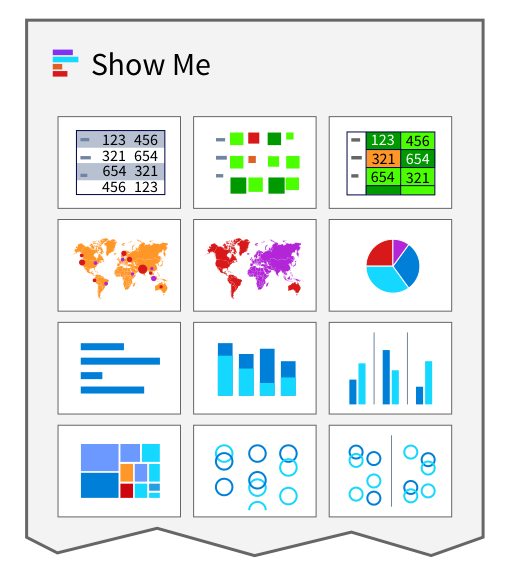
\includegraphics[width=0.95\textwidth,height=0.75\textheight,keepaspectratio]{../textbookForPractice/Figures/Ch_03/ILLUSTRATION 3.43.png}
    \end{figure}
\end{frame}

\begin{frame}{ILLUSTRATION 3.44}

    \begin{figure}[h]
        \centering
        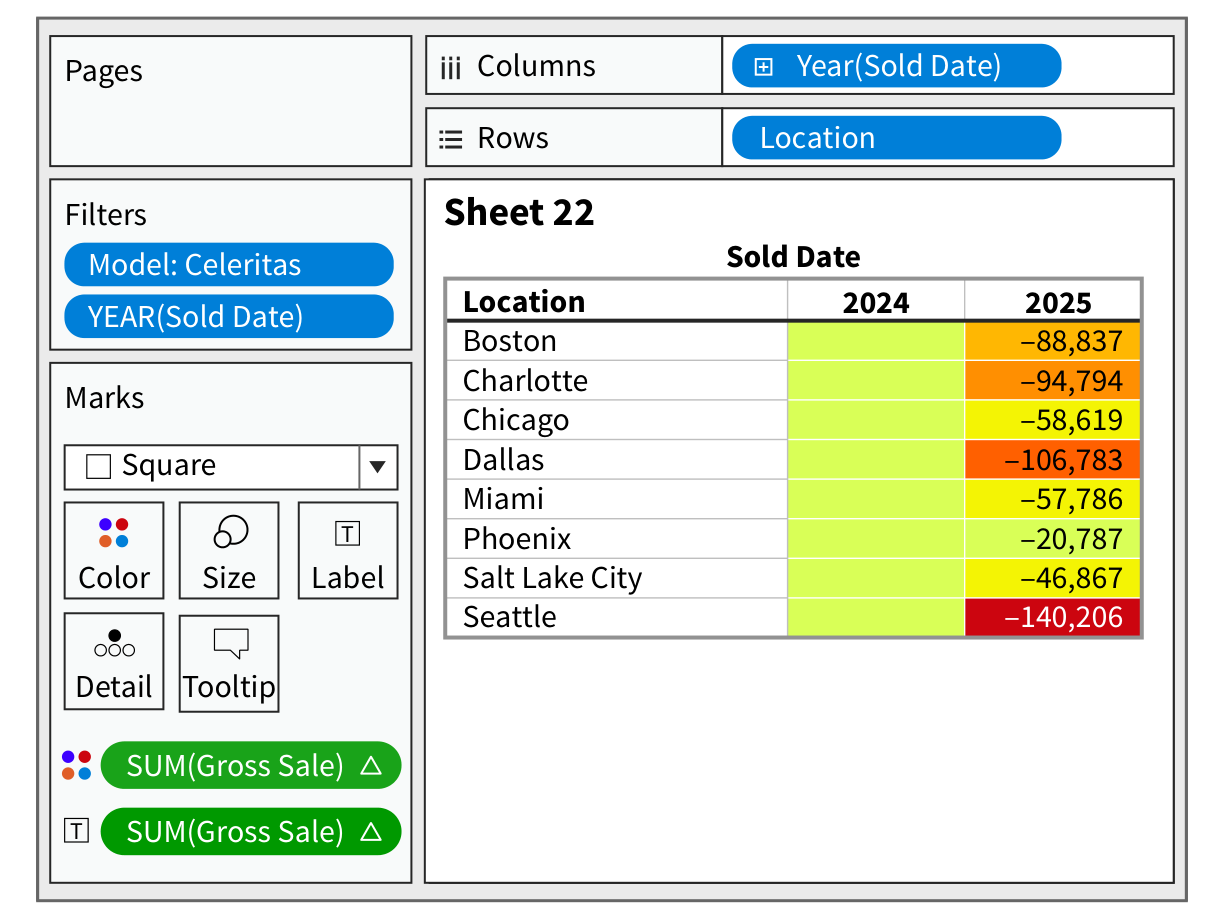
\includegraphics[width=0.95\textwidth,height=0.75\textheight,keepaspectratio]{../textbookForPractice/Figures/Ch_03/ILLUSTRATION 3.44.png}
    \end{figure}
\end{frame}

\begin{frame}{ILLUSTRATION 3.45}

    \begin{figure}[h]
        \centering
        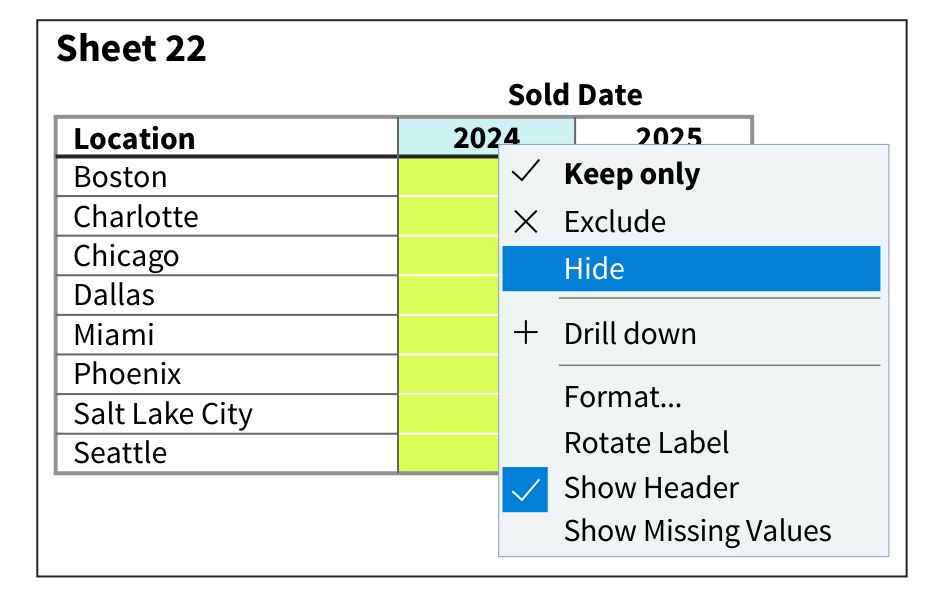
\includegraphics[width=0.95\textwidth,height=0.75\textheight,keepaspectratio]{../textbookForPractice/Figures/Ch_03/ILLUSTRATION 3.45.png}
    \end{figure}
\end{frame}

\begin{frame}{ILLUSTRATION 3.46}

    \begin{figure}[h]
        \centering
        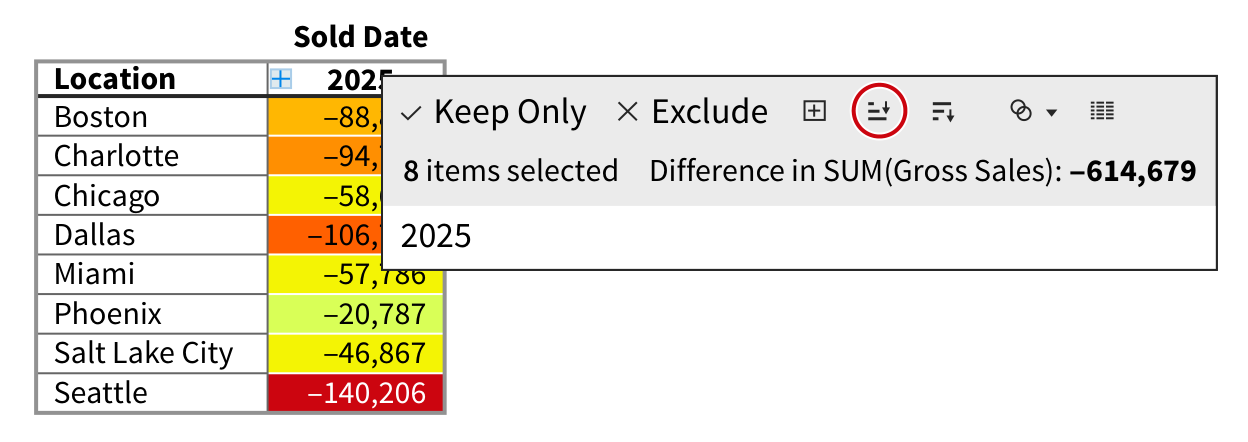
\includegraphics[width=0.95\textwidth,height=0.75\textheight,keepaspectratio]{../textbookForPractice/Figures/Ch_03/ILLUSTRATION 3.46.png}
    \end{figure}
\end{frame}

\begin{frame}{ILLUSTRATION 3.47}

    \begin{figure}[h]
        \centering
        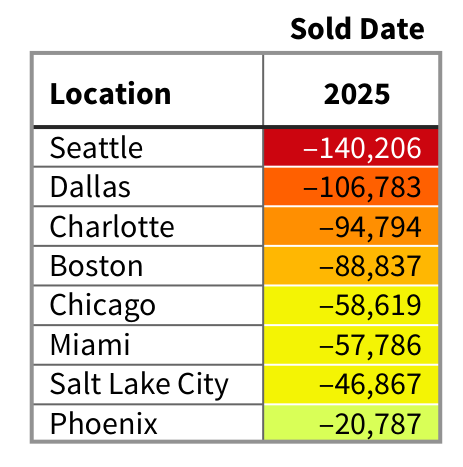
\includegraphics[width=0.95\textwidth,height=0.75\textheight,keepaspectratio]{../textbookForPractice/Figures/Ch_03/ILLUSTRATION 3.47.png}
    \end{figure}
\end{frame}

\begin{frame}{ILLUSTRATION 3.48}

    \begin{figure}[h]
        \centering
        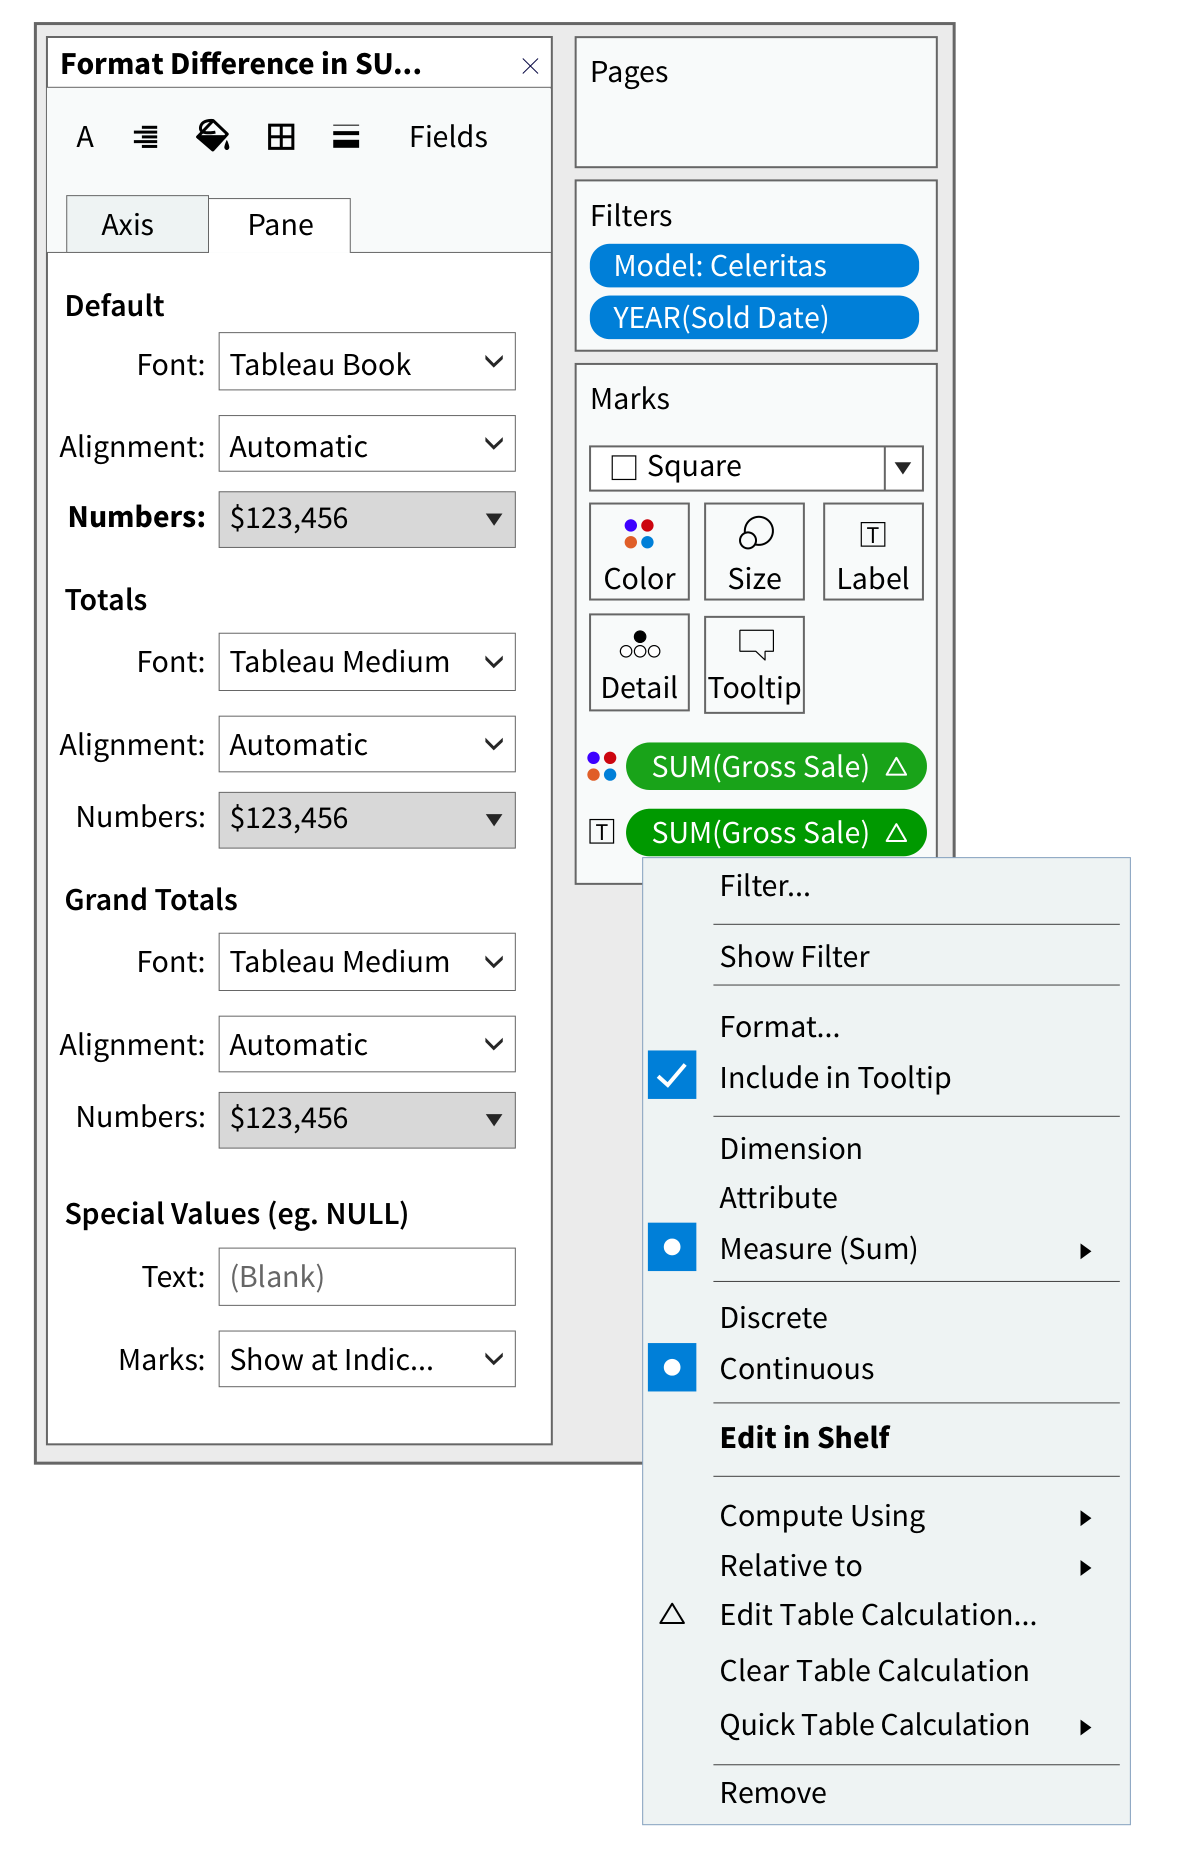
\includegraphics[width=0.95\textwidth,height=0.75\textheight,keepaspectratio]{../textbookForPractice/Figures/Ch_03/ILLUSTRATION 3.48.png}
    \end{figure}
\end{frame}

\begin{frame}{ILLUSTRATION 3.49}

    \begin{figure}[h]
        \centering
        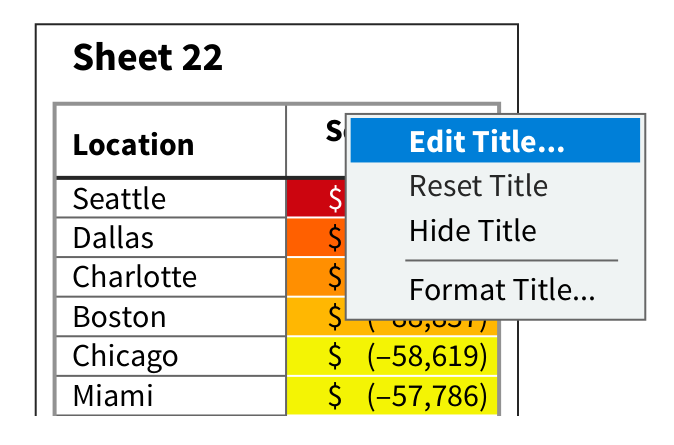
\includegraphics[width=0.95\textwidth,height=0.75\textheight,keepaspectratio]{../textbookForPractice/Figures/Ch_03/ILLUSTRATION 3.49.png}
    \end{figure}
\end{frame}

\begin{frame}{ILLUSTRATION 3.50}

    \begin{figure}[h]
        \centering
        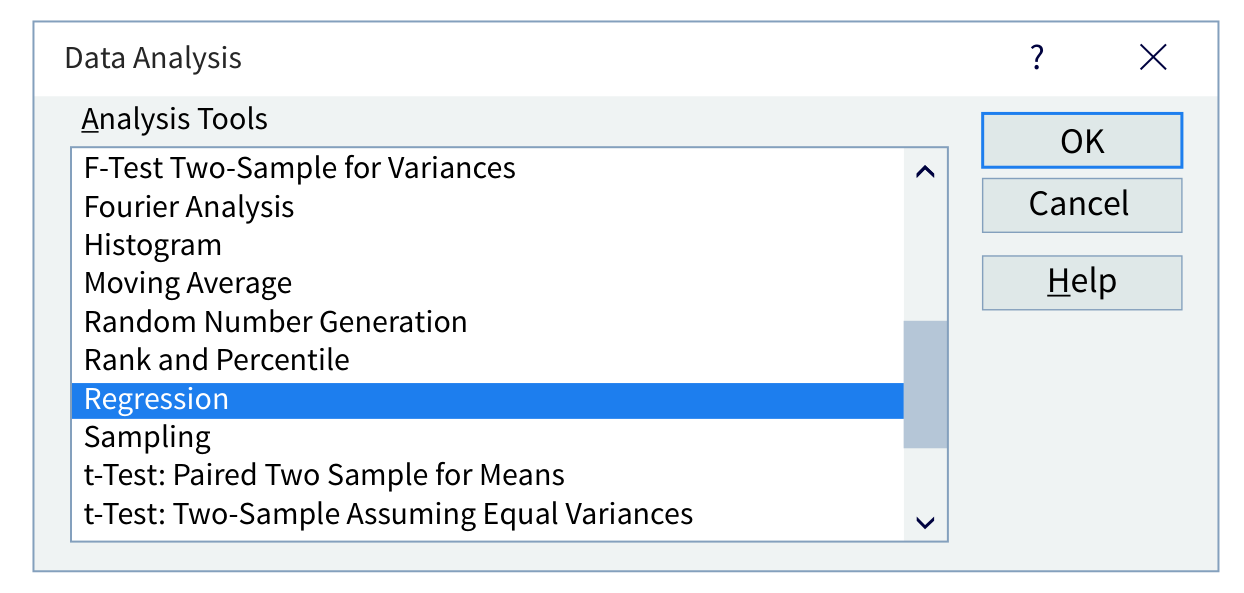
\includegraphics[width=0.95\textwidth,height=0.75\textheight,keepaspectratio]{../textbookForPractice/Figures/Ch_03/ILLUSTRATION 3.50.png}
    \end{figure}
\end{frame}

\begin{frame}{ILLUSTRATION 3.50\_1}

    \begin{figure}[h]
        \centering
        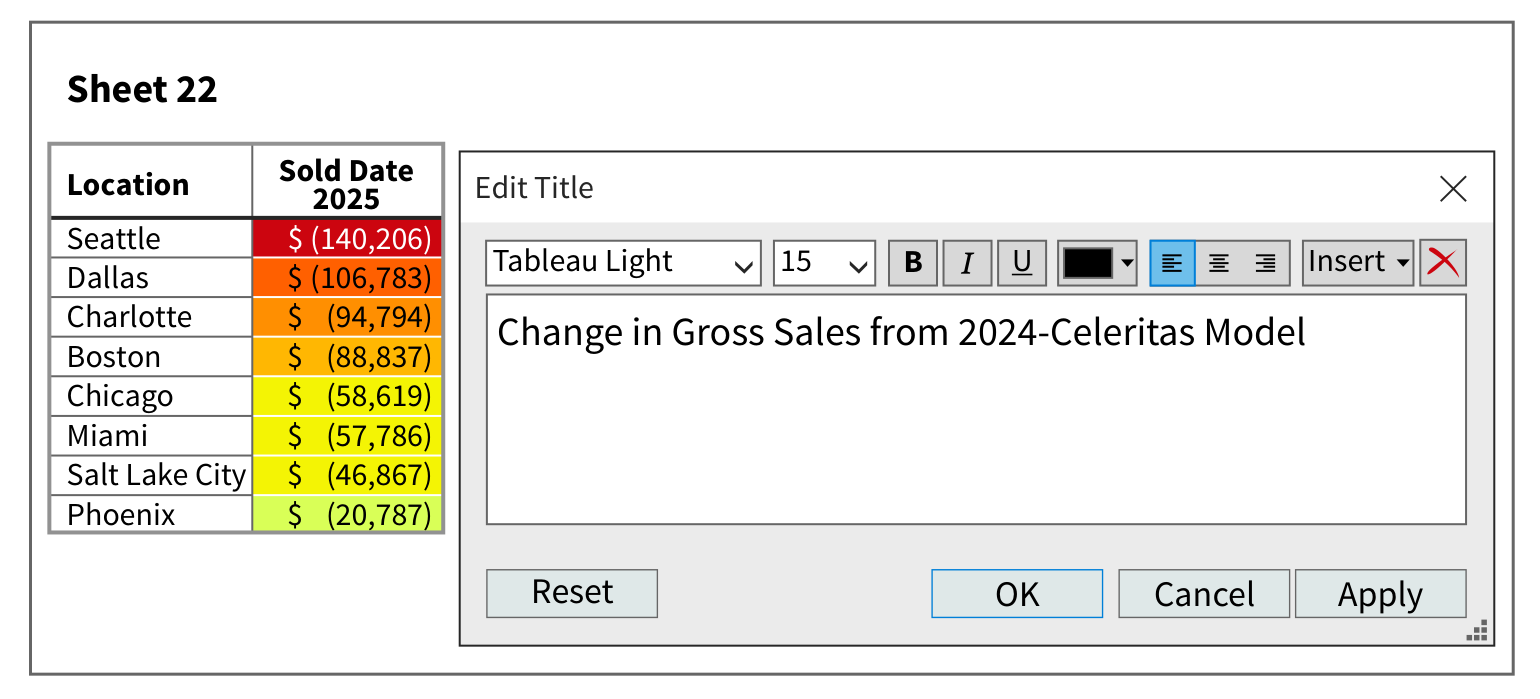
\includegraphics[width=0.95\textwidth,height=0.75\textheight,keepaspectratio]{../textbookForPractice/Figures/Ch_03/ILLUSTRATION 3.50_1.png}
    \end{figure}
\end{frame}

\begin{frame}{ILLUSTRATION 3.51}

    \begin{figure}[h]
        \centering
        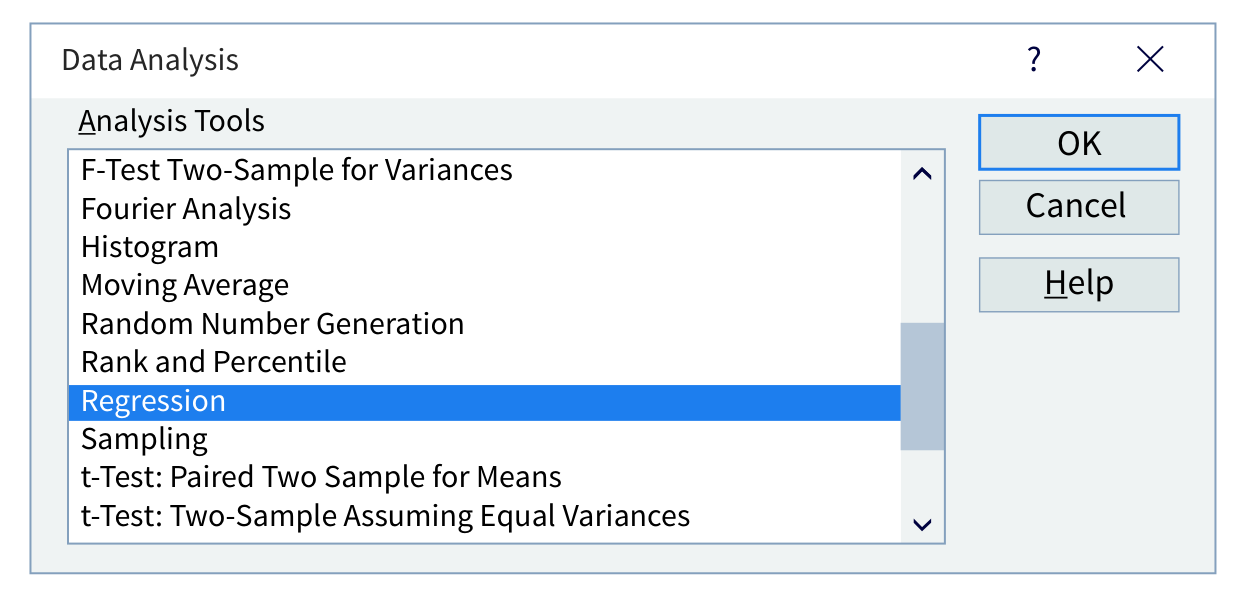
\includegraphics[width=0.95\textwidth,height=0.75\textheight,keepaspectratio]{../textbookForPractice/Figures/Ch_03/ILLUSTRATION 3.51.png}
    \end{figure}
\end{frame}

\begin{frame}{ILLUSTRATION 3.52}

    \begin{figure}[h]
        \centering
        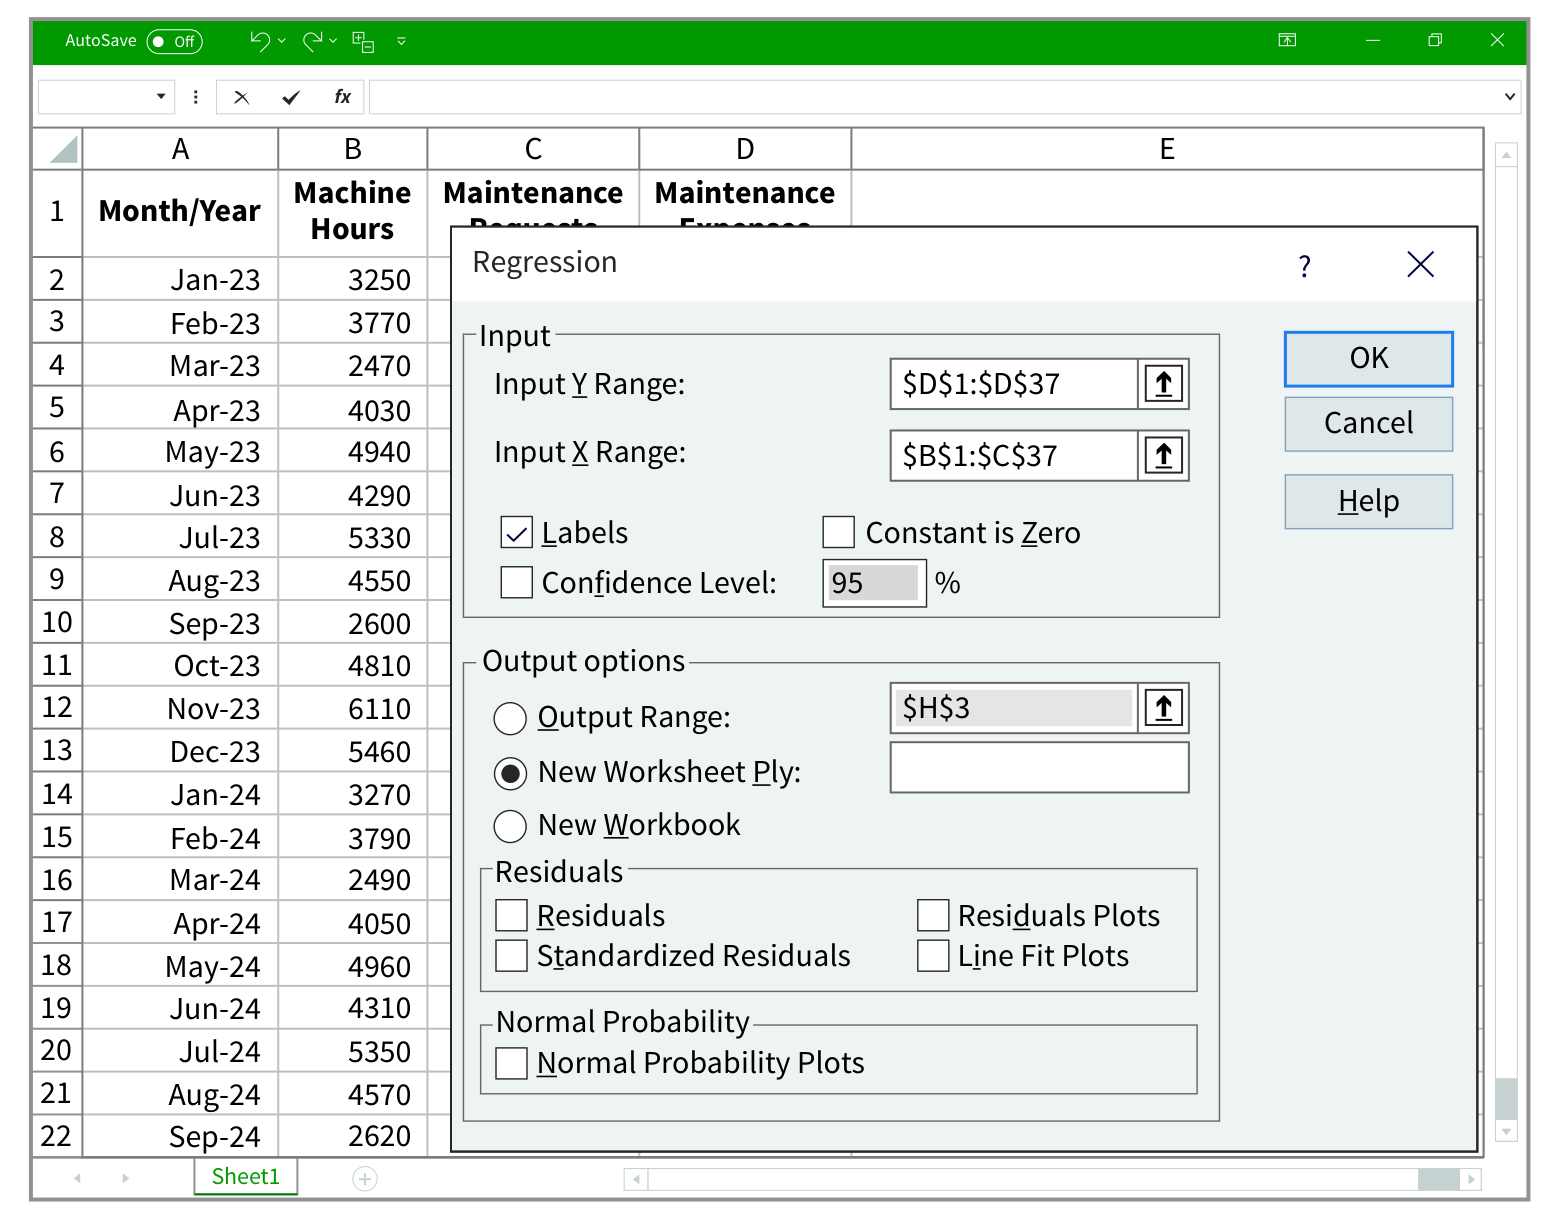
\includegraphics[width=0.95\textwidth,height=0.75\textheight,keepaspectratio]{../textbookForPractice/Figures/Ch_03/ILLUSTRATION 3.52.png}
    \end{figure}
\end{frame}

\begin{frame}{ILLUSTRATION 3.53}

    \begin{figure}[h]
        \centering
        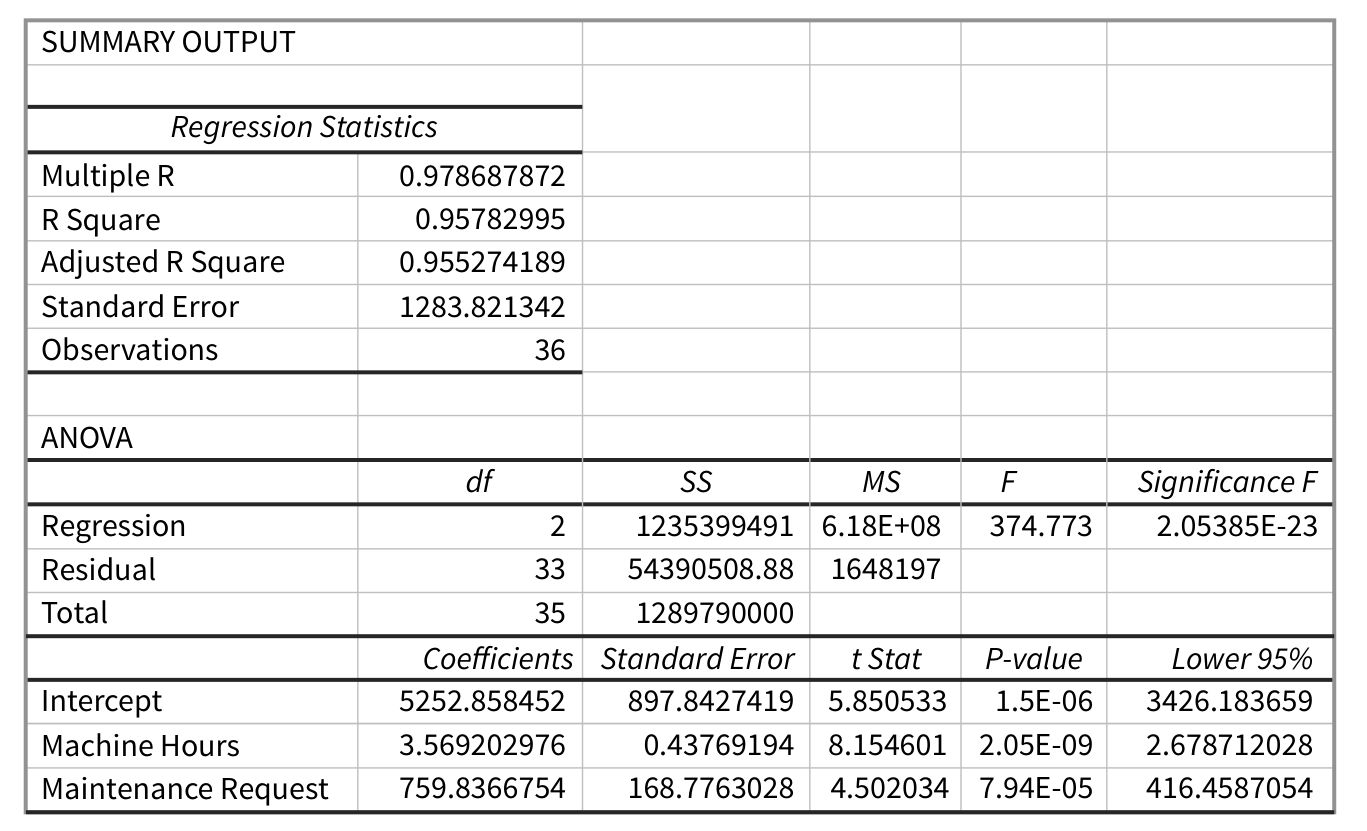
\includegraphics[width=0.95\textwidth,height=0.75\textheight,keepaspectratio]{../textbookForPractice/Figures/Ch_03/ILLUSTRATION 3.53.png}
    \end{figure}
\end{frame}

\begin{frame}{Bài tập Ngắn (Brief Exercises)}
\begin{center}
    \Huge \textbf{Phần Bài tập Ngắn} \\
    \vspace{0.5cm}
    \Large Brief Exercises (BE)
\end{center}
\end{frame}

\begin{frame}{BE 3.1 \& BE 3.2}
    \begin{columns}
        \begin{column}{0.5\textwidth}
            \begin{figure}[h]
                \centering
                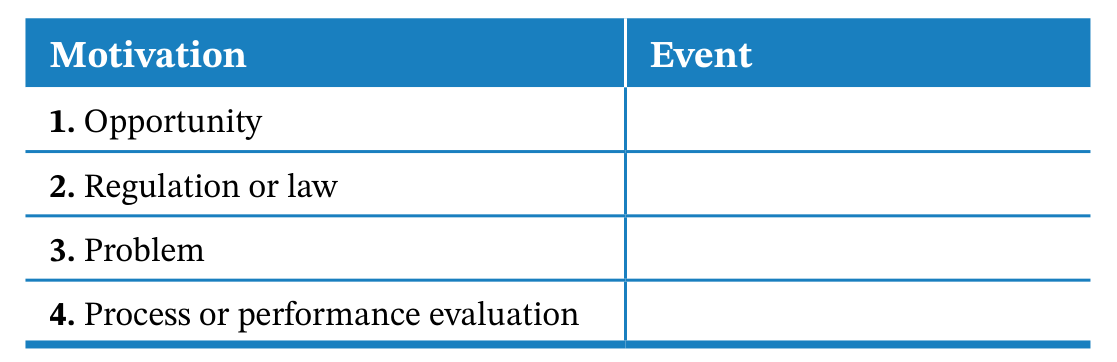
\includegraphics[width=\textwidth,height=0.7\textheight,keepaspectratio]{../textbookForPractice/Figures/Ch_03/BE 3.1.png}
            \end{figure}
        \end{column}
        \begin{column}{0.5\textwidth}
            \begin{figure}[h]
                \centering
                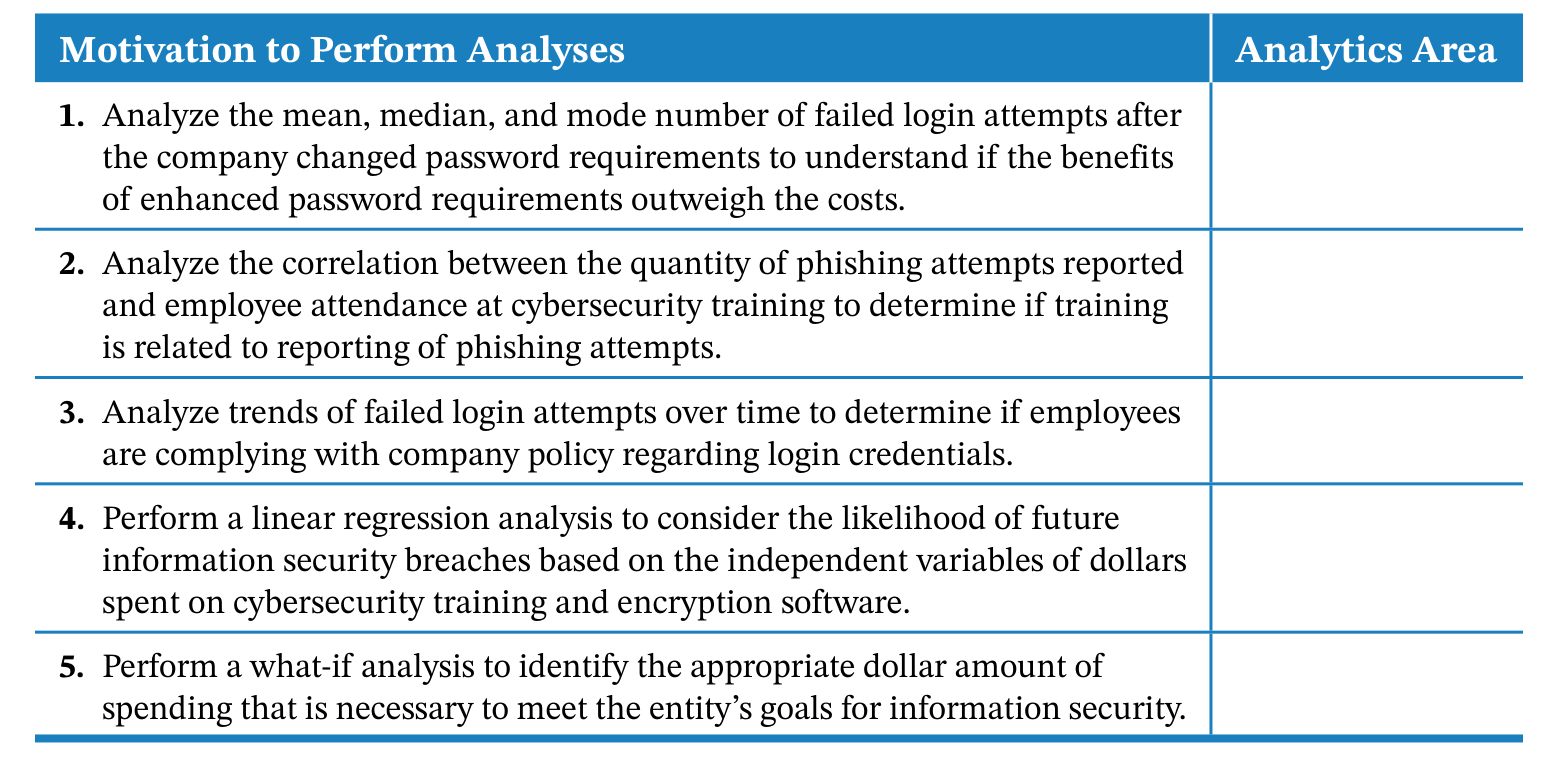
\includegraphics[width=\textwidth,height=0.7\textheight,keepaspectratio]{../textbookForPractice/Figures/Ch_03/BE 3.2.png}
            \end{figure}
        \end{column}
    \end{columns}
\end{frame}

\begin{frame}{BE 3.3 \& BE 3.5}
    \begin{columns}
        \begin{column}{0.5\textwidth}
            \begin{figure}[h]
                \centering
                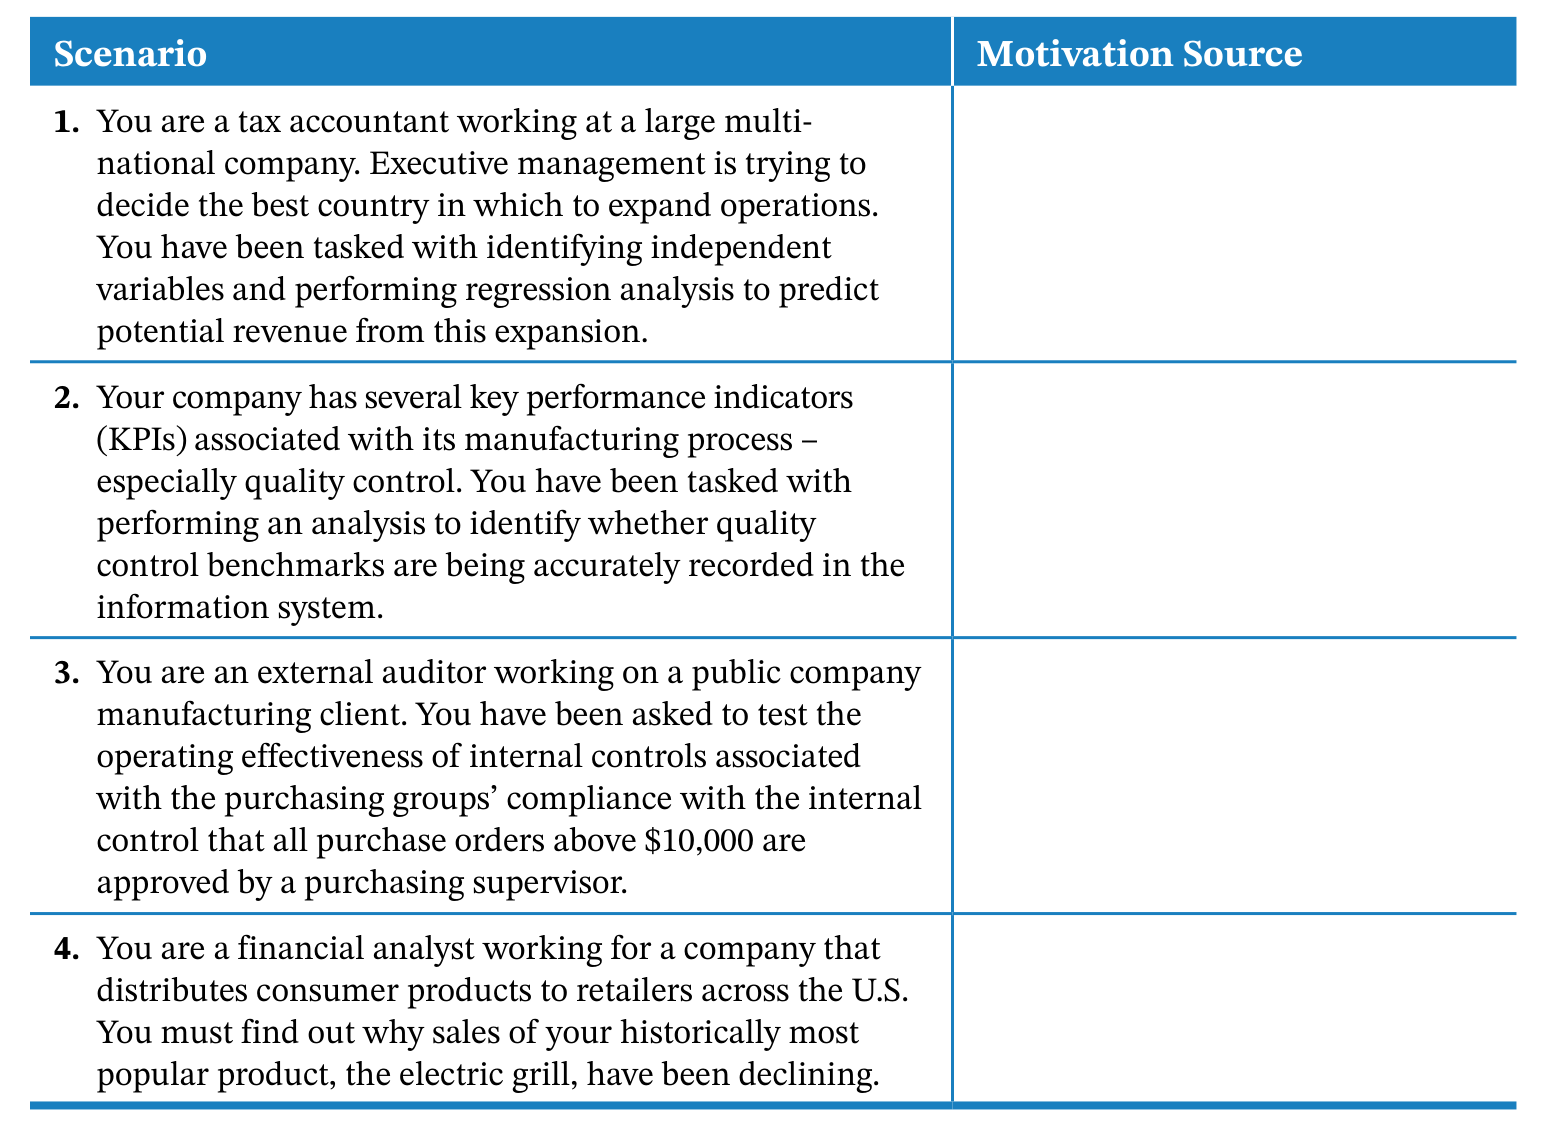
\includegraphics[width=\textwidth,height=0.7\textheight,keepaspectratio]{../textbookForPractice/Figures/Ch_03/BE 3.3.png}
            \end{figure}
        \end{column}
        \begin{column}{0.5\textwidth}
            \begin{figure}[h]
                \centering
                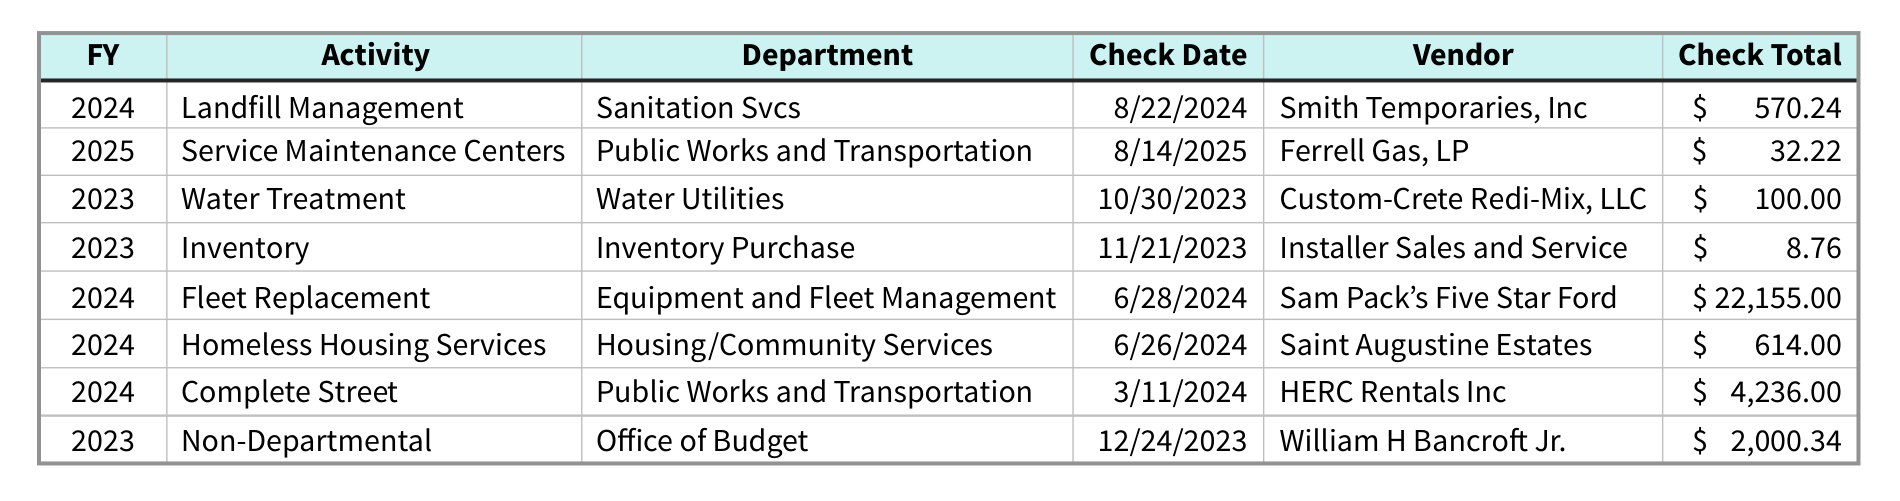
\includegraphics[width=\textwidth,height=0.7\textheight,keepaspectratio]{../textbookForPractice/Figures/Ch_03/BE 3.5.png}
            \end{figure}
        \end{column}
    \end{columns}
\end{frame}

\begin{frame}{BE 3.6 \& BE 3.7}
    \begin{columns}
        \begin{column}{0.5\textwidth}
            \begin{figure}[h]
                \centering
                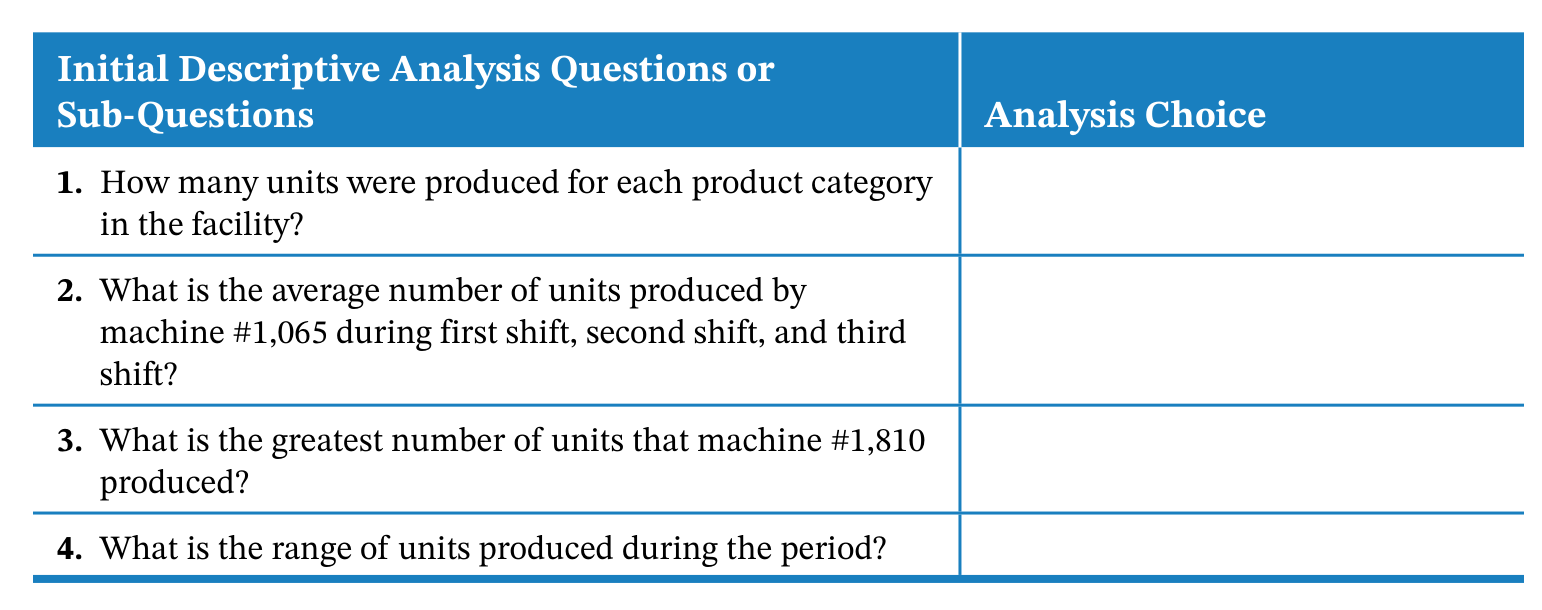
\includegraphics[width=\textwidth,height=0.7\textheight,keepaspectratio]{../textbookForPractice/Figures/Ch_03/BE 3.6.png}
            \end{figure}
        \end{column}
        \begin{column}{0.5\textwidth}
            \begin{figure}[h]
                \centering
                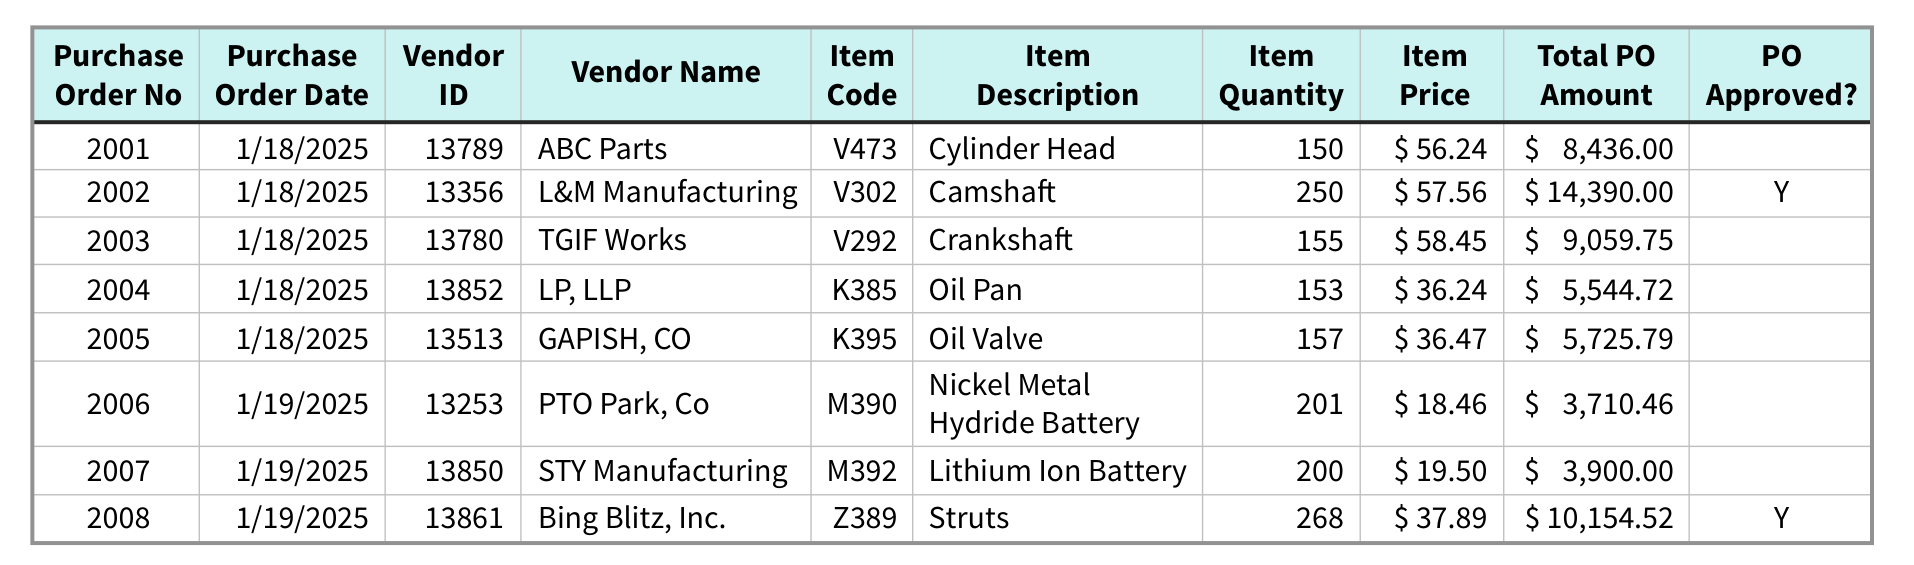
\includegraphics[width=\textwidth,height=0.7\textheight,keepaspectratio]{../textbookForPractice/Figures/Ch_03/BE 3.7.png}
            \end{figure}
        \end{column}
    \end{columns}
\end{frame}

\begin{frame}{BE 3.8 \& BE 3.9}
    \begin{columns}
        \begin{column}{0.5\textwidth}
            \begin{figure}[h]
                \centering
                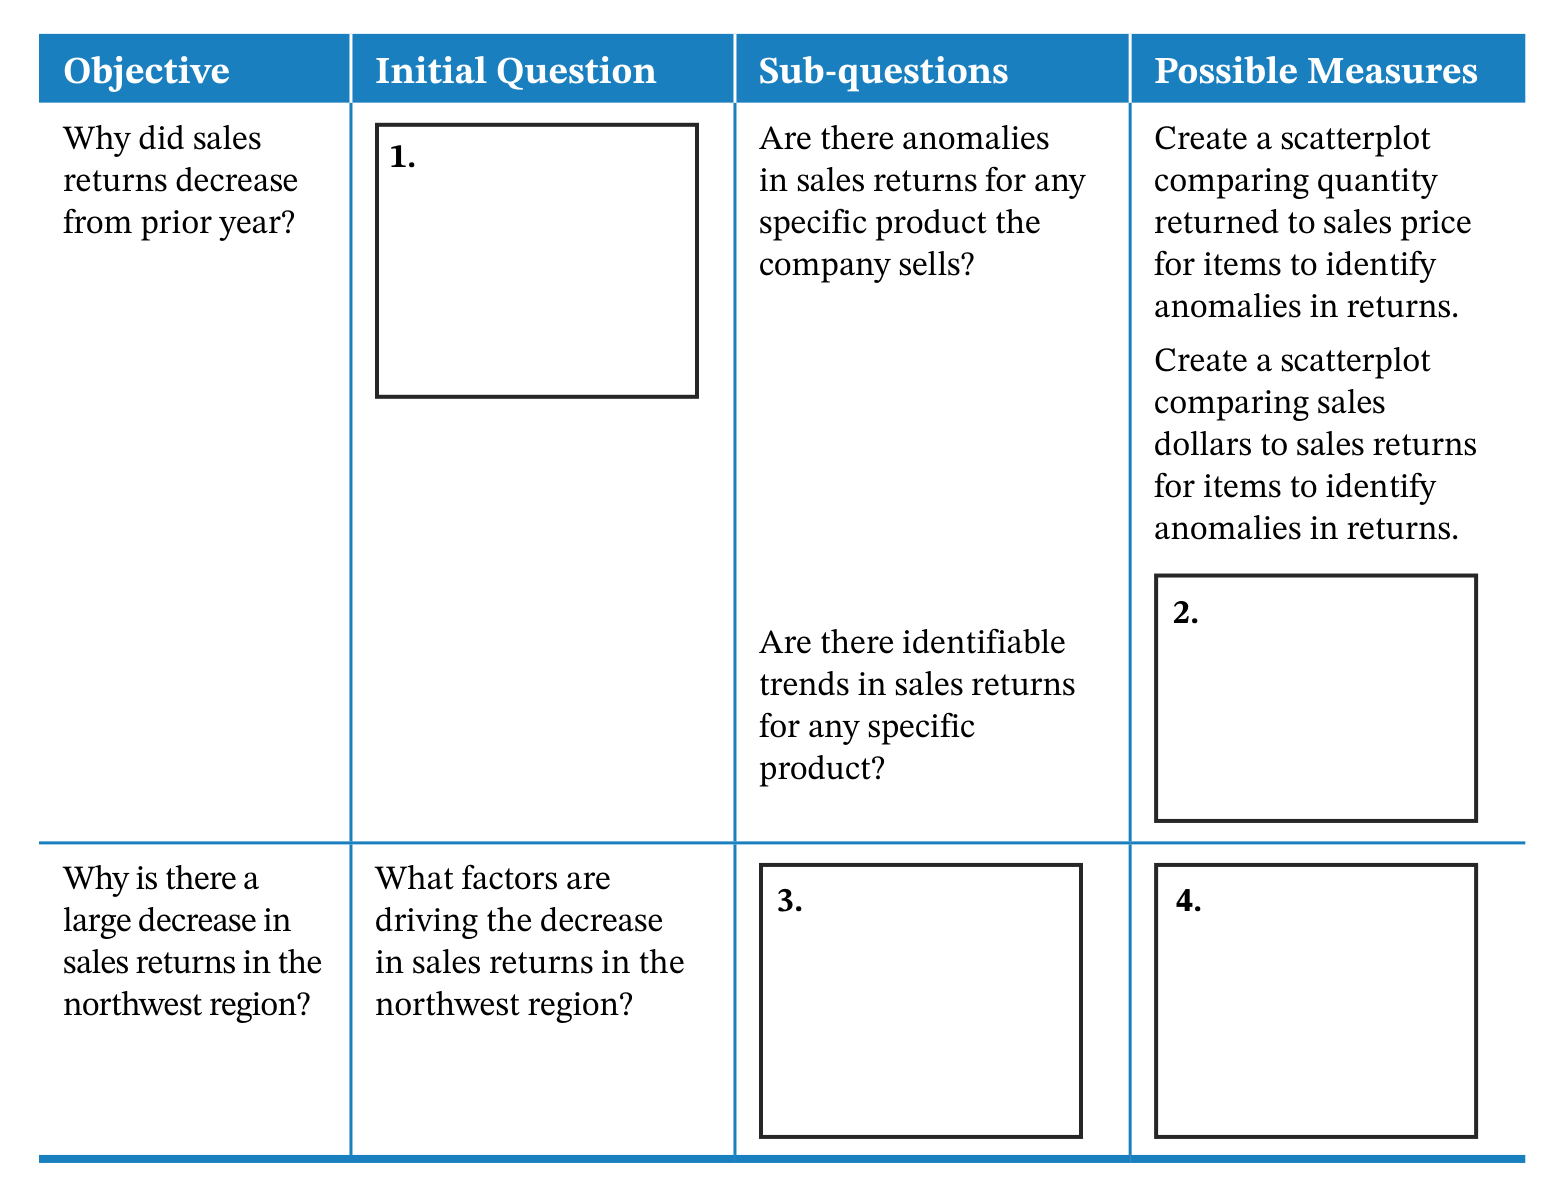
\includegraphics[width=\textwidth,height=0.7\textheight,keepaspectratio]{../textbookForPractice/Figures/Ch_03/BE 3.8.png}
            \end{figure}
        \end{column}
        \begin{column}{0.5\textwidth}
            \begin{figure}[h]
                \centering
                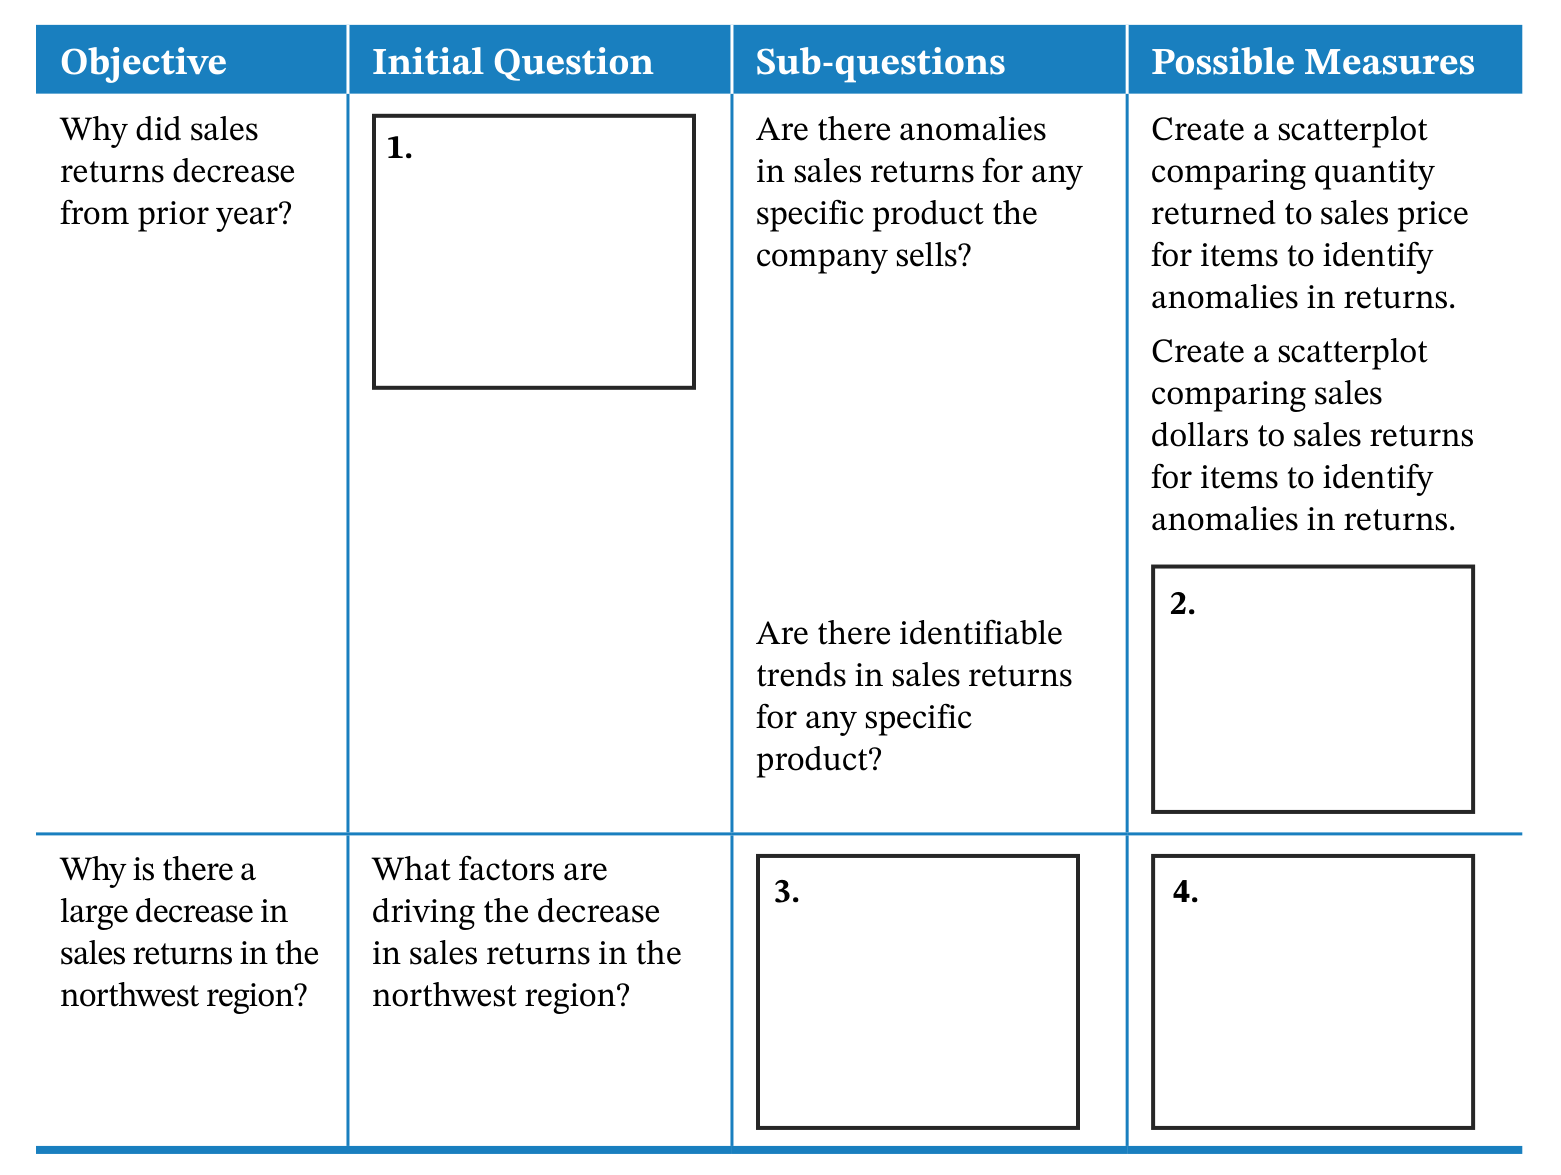
\includegraphics[width=\textwidth,height=0.7\textheight,keepaspectratio]{../textbookForPractice/Figures/Ch_03/BE 3.9.png}
            \end{figure}
        \end{column}
    \end{columns}
\end{frame}

\begin{frame}{BE 3.9\_1 \& BE 3.11}
    \begin{columns}
        \begin{column}{0.5\textwidth}
            \begin{figure}[h]
                \centering
                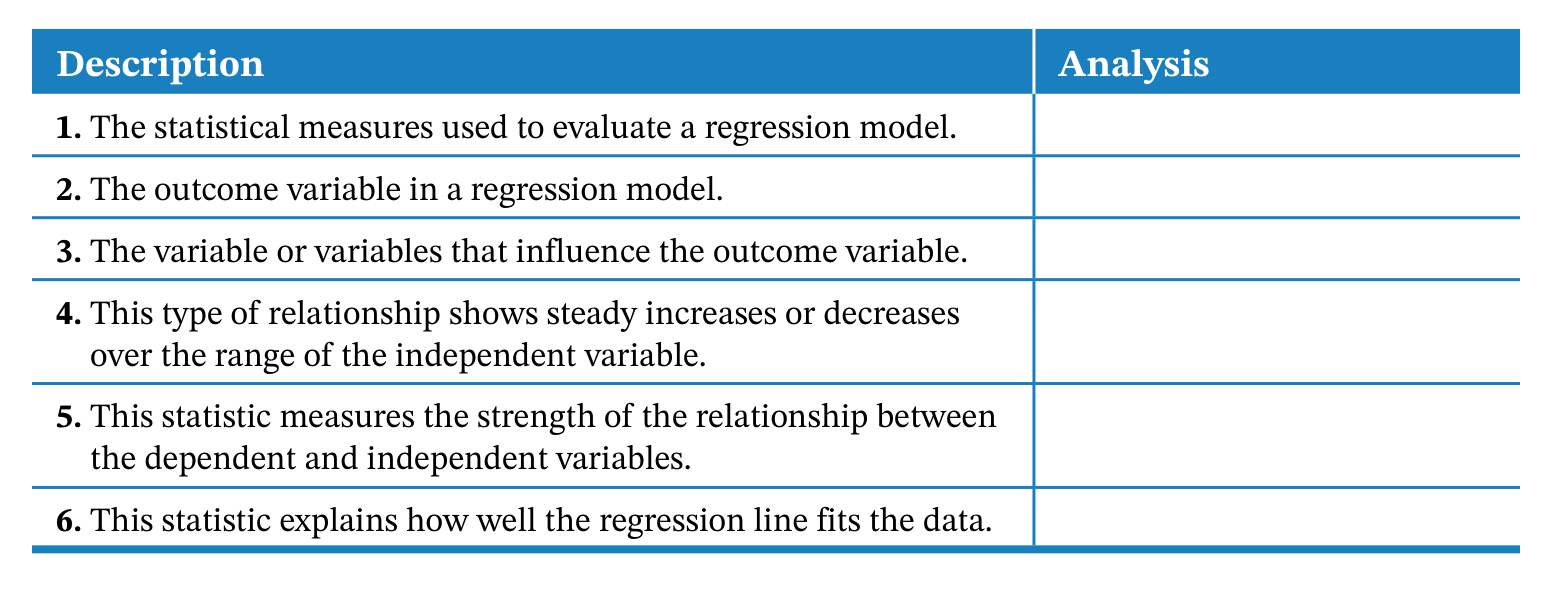
\includegraphics[width=\textwidth,height=0.7\textheight,keepaspectratio]{../textbookForPractice/Figures/Ch_03/BE 3.9_1.png}
            \end{figure}
        \end{column}
        \begin{column}{0.5\textwidth}
            \begin{figure}[h]
                \centering
                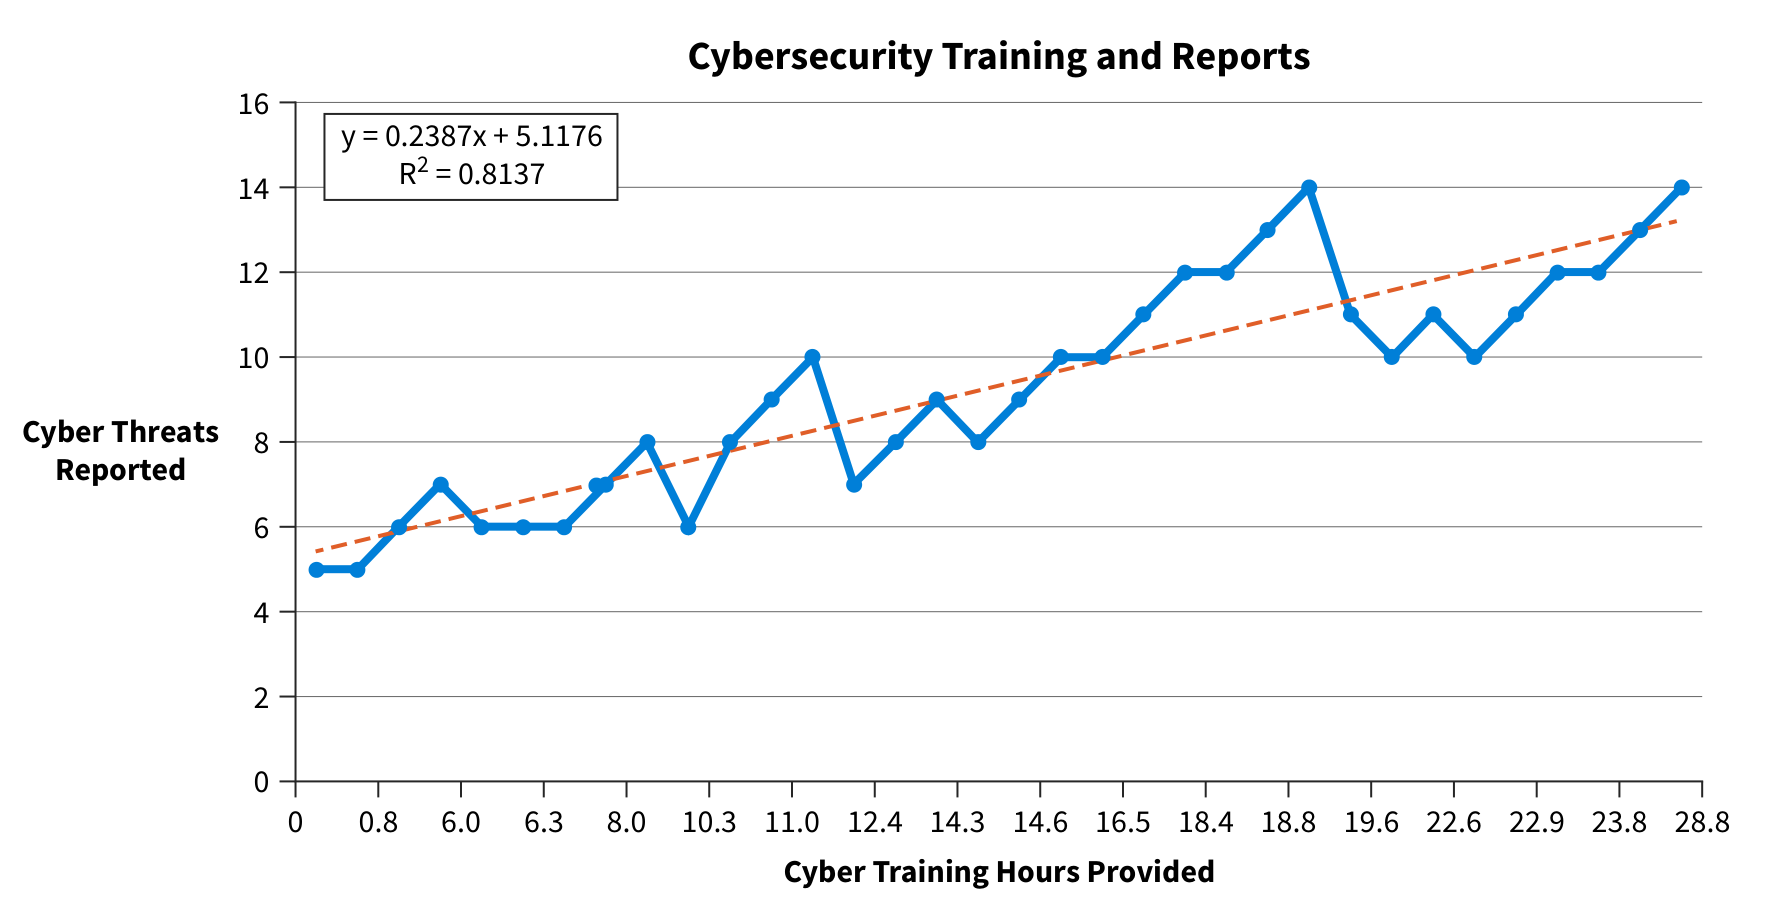
\includegraphics[width=\textwidth,height=0.7\textheight,keepaspectratio]{../textbookForPractice/Figures/Ch_03/BE 3.11.png}
            \end{figure}
        \end{column}
    \end{columns}
\end{frame}

\begin{frame}{BE 3.12 \& BE 3.13}
    \begin{columns}
        \begin{column}{0.5\textwidth}
            \begin{figure}[h]
                \centering
                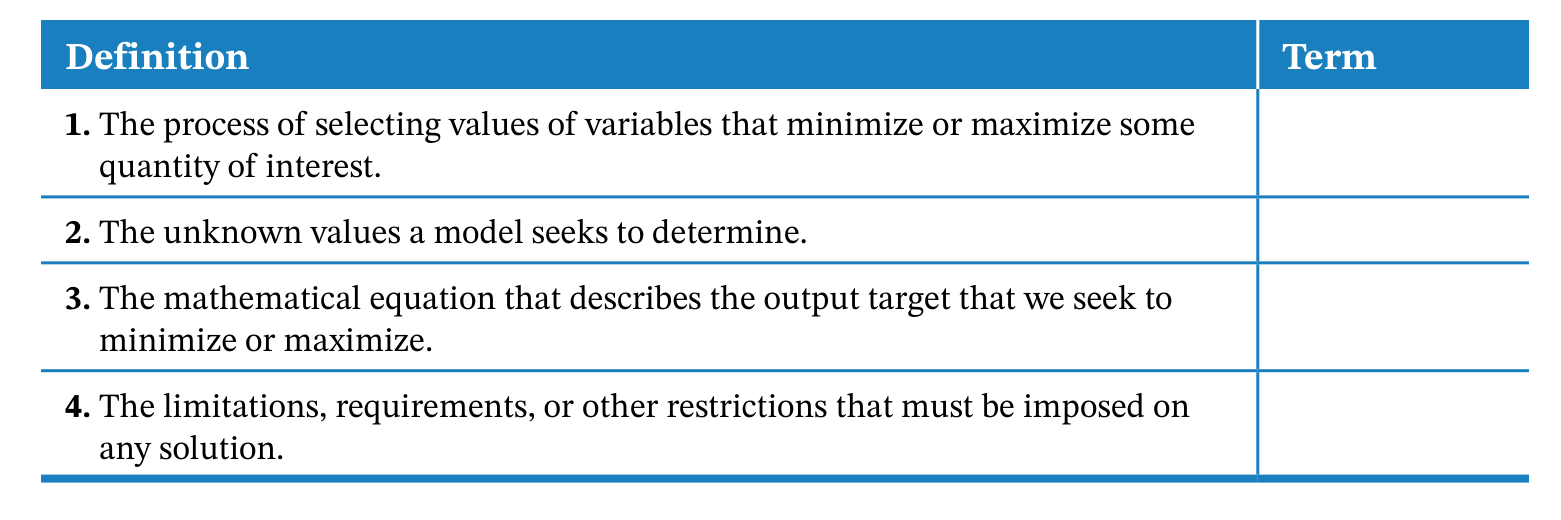
\includegraphics[width=\textwidth,height=0.7\textheight,keepaspectratio]{../textbookForPractice/Figures/Ch_03/BE 3.12.png}
            \end{figure}
        \end{column}
        \begin{column}{0.5\textwidth}
            \begin{figure}[h]
                \centering
                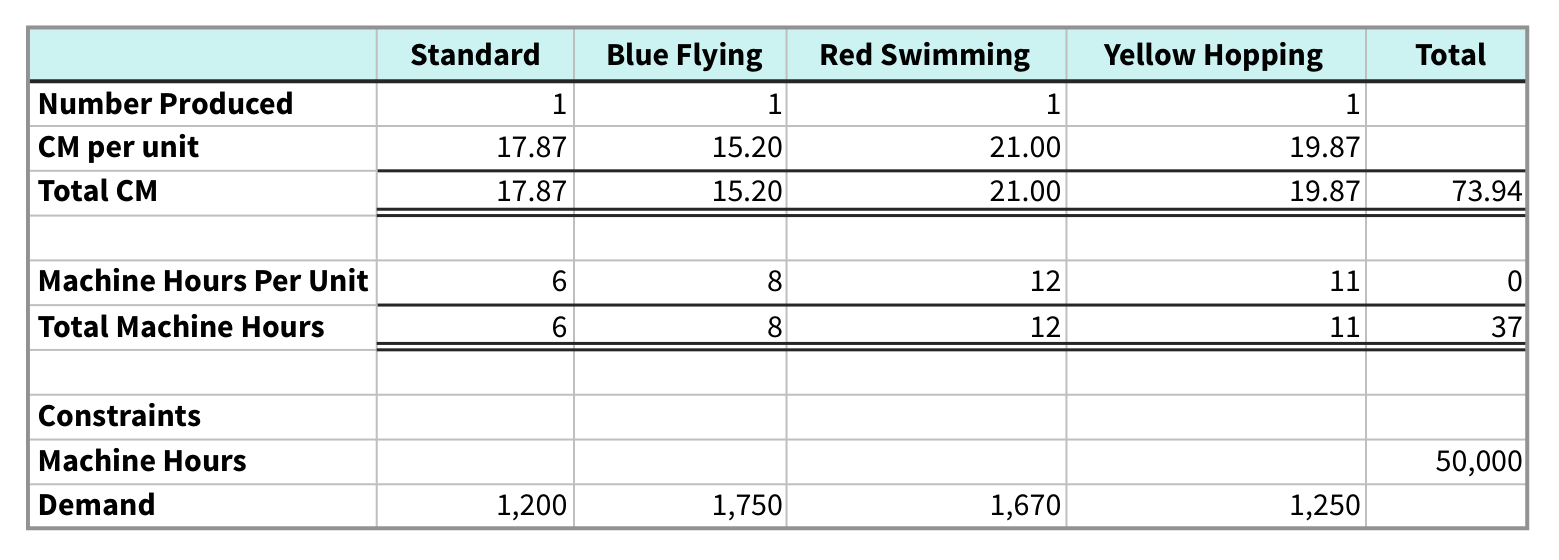
\includegraphics[width=\textwidth,height=0.7\textheight,keepaspectratio]{../textbookForPractice/Figures/Ch_03/BE 3.13.png}
            \end{figure}
        \end{column}
    \end{columns}
\end{frame}

\begin{frame}{BE 3.13\_1 \& BE 3.16}
    \begin{columns}
        \begin{column}{0.5\textwidth}
            \begin{figure}[h]
                \centering
                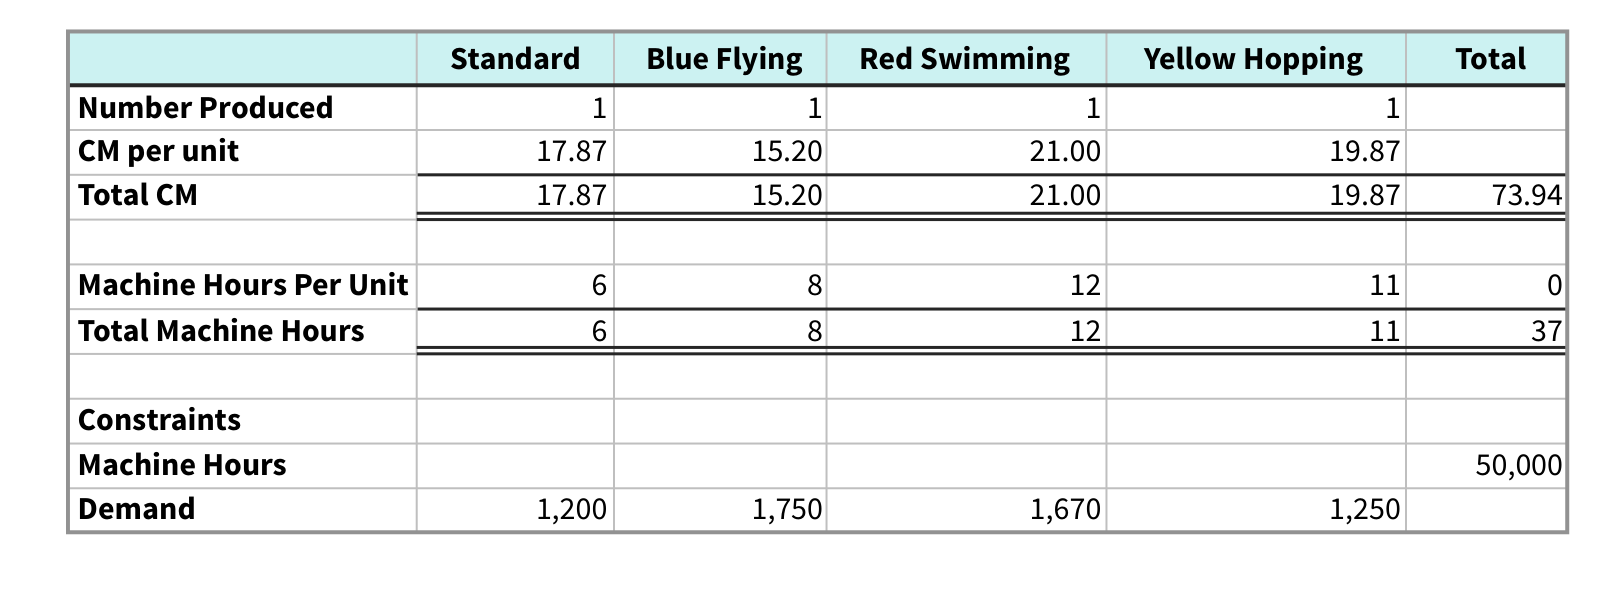
\includegraphics[width=\textwidth,height=0.7\textheight,keepaspectratio]{../textbookForPractice/Figures/Ch_03/BE 3.13_1.png}
            \end{figure}
        \end{column}
        \begin{column}{0.5\textwidth}
            \begin{figure}[h]
                \centering
                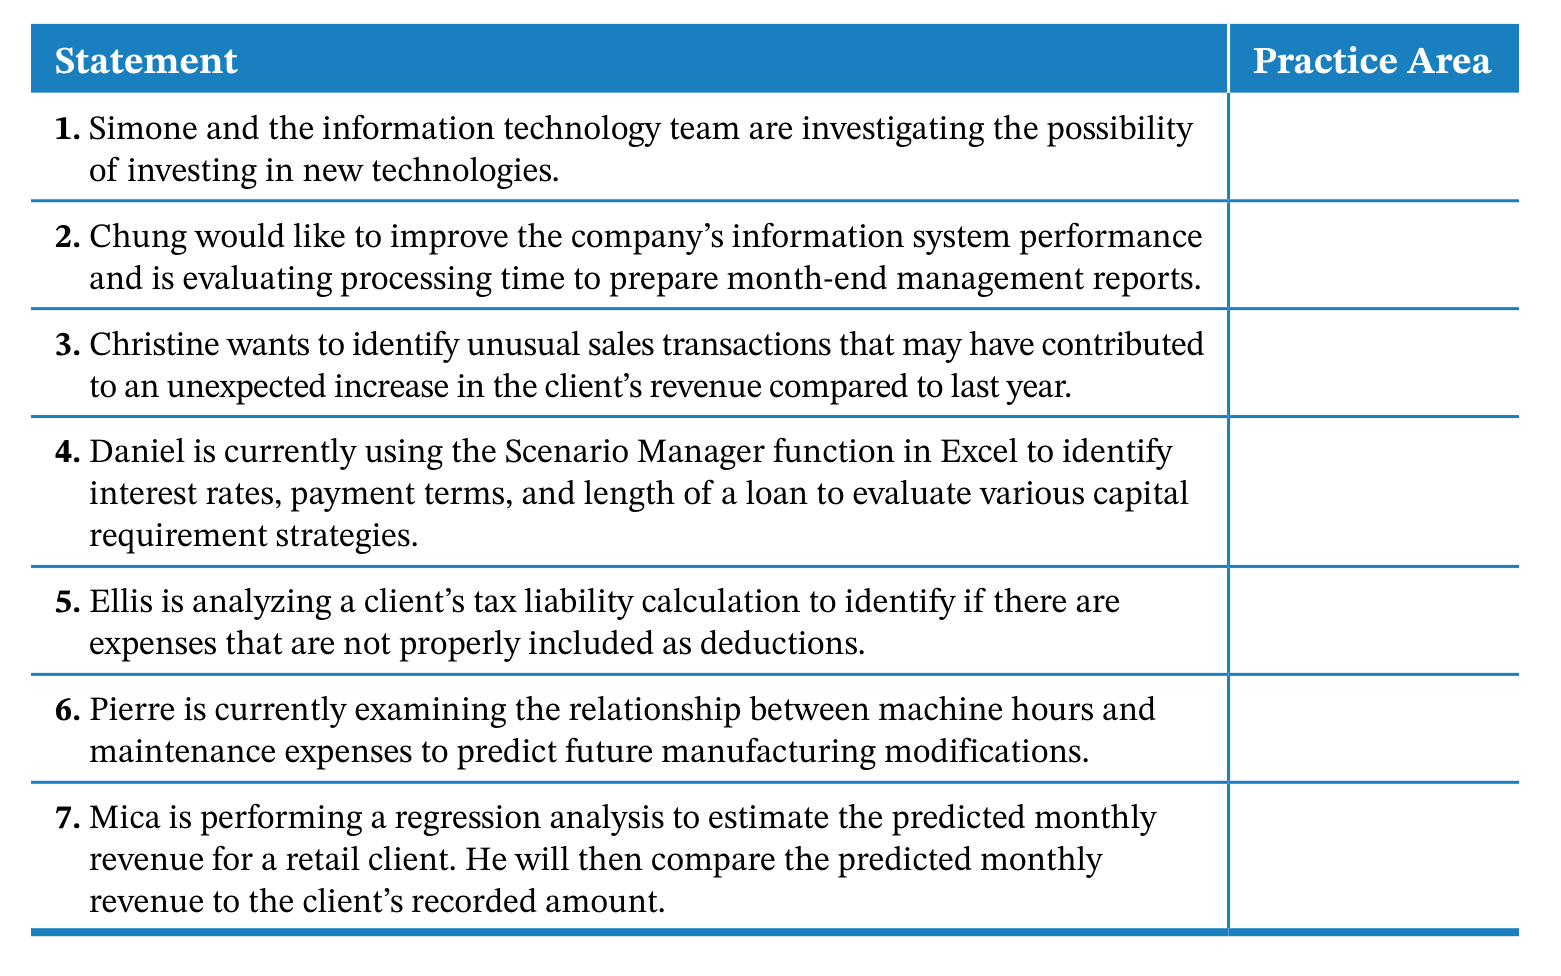
\includegraphics[width=\textwidth,height=0.7\textheight,keepaspectratio]{../textbookForPractice/Figures/Ch_03/BE 3.16.png}
            \end{figure}
        \end{column}
    \end{columns}
\end{frame}

\begin{frame}{Bài tập (Exercises)}
\begin{center}
    \Huge \textbf{Phần Bài tập} \\
    \vspace{0.5cm}
    \Large Exercises (EX)
\end{center}
\end{frame}

\begin{frame}{EX 3.1 \& EX 3.4}
    \begin{columns}
        \begin{column}{0.5\textwidth}
            \begin{figure}[h]
                \centering
                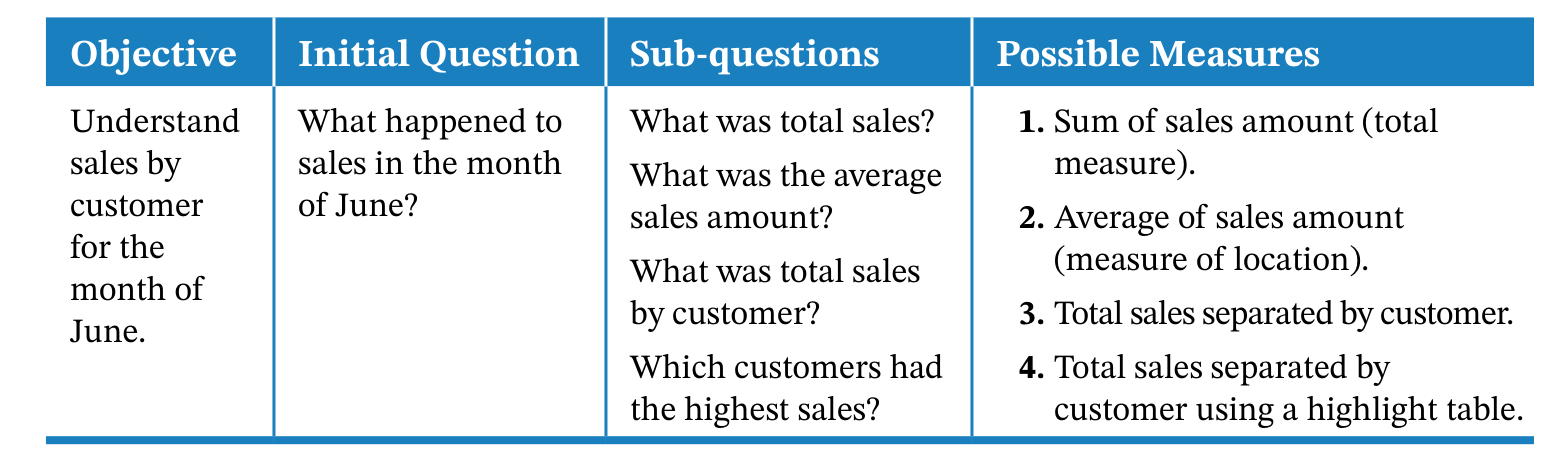
\includegraphics[width=\textwidth,height=0.7\textheight,keepaspectratio]{../textbookForPractice/Figures/Ch_03/EX 3.1.png}
            \end{figure}
        \end{column}
        \begin{column}{0.5\textwidth}
            \begin{figure}[h]
                \centering
                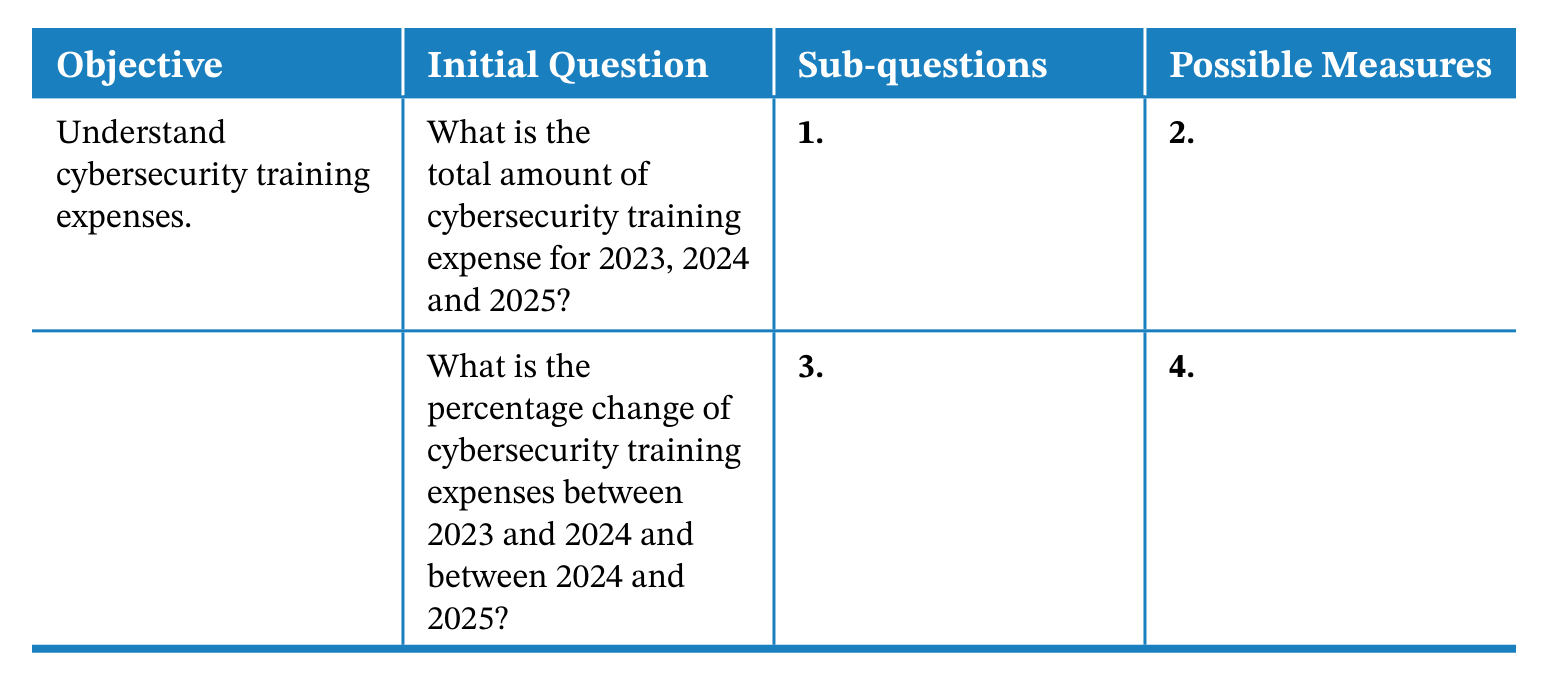
\includegraphics[width=\textwidth,height=0.7\textheight,keepaspectratio]{../textbookForPractice/Figures/Ch_03/EX 3.4.png}
            \end{figure}
        \end{column}
    \end{columns}
\end{frame}

\begin{frame}{EX 3.7A \& EX 3.7B}
    \begin{columns}
        \begin{column}{0.5\textwidth}
            \begin{figure}[h]
                \centering
                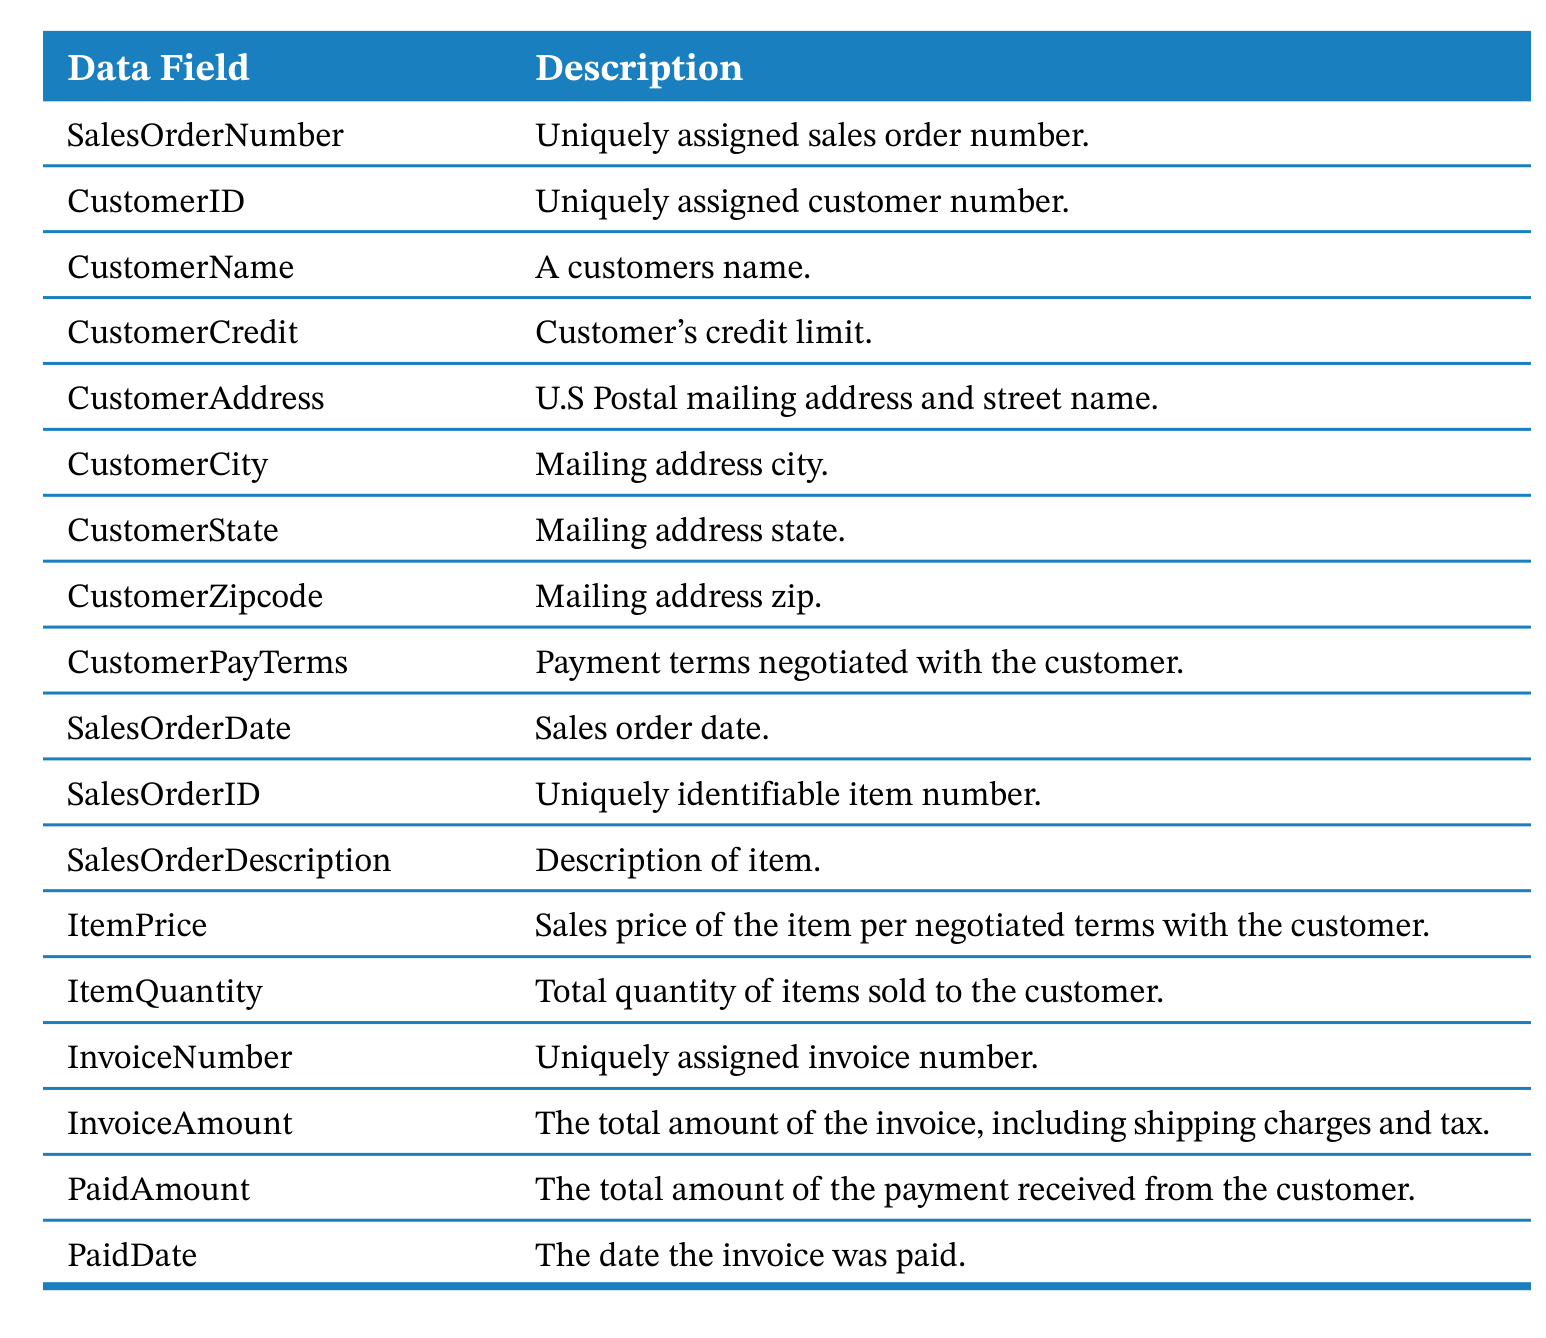
\includegraphics[width=\textwidth,height=0.7\textheight,keepaspectratio]{../textbookForPractice/Figures/Ch_03/EX 3.7A.png}
            \end{figure}
        \end{column}
        \begin{column}{0.5\textwidth}
            \begin{figure}[h]
                \centering
                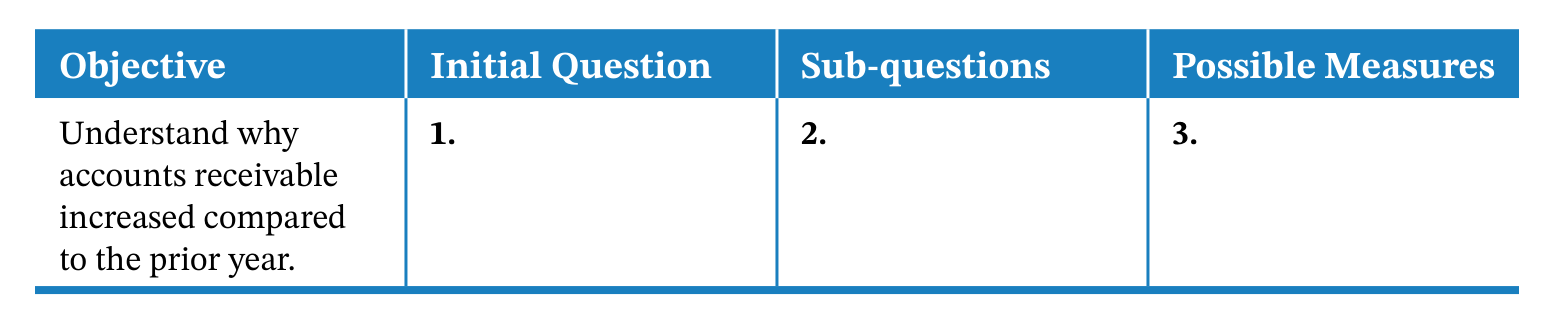
\includegraphics[width=\textwidth,height=0.7\textheight,keepaspectratio]{../textbookForPractice/Figures/Ch_03/EX 3.7B.png}
            \end{figure}
        \end{column}
    \end{columns}
\end{frame}

\begin{frame}{EX 3.8 \& EX 3.8\_1}
    \begin{columns}
        \begin{column}{0.5\textwidth}
            \begin{figure}[h]
                \centering
                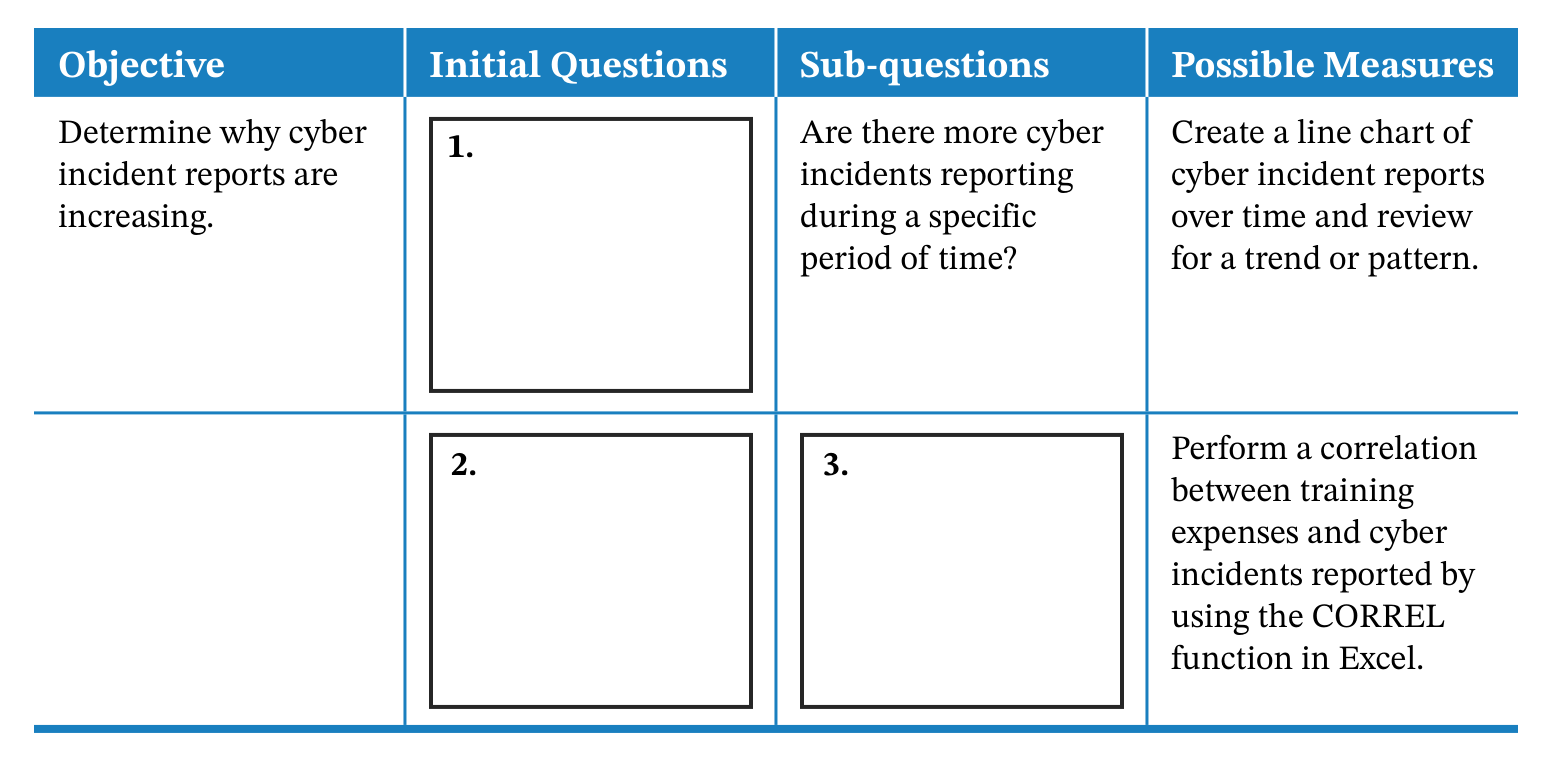
\includegraphics[width=\textwidth,height=0.7\textheight,keepaspectratio]{../textbookForPractice/Figures/Ch_03/EX 3.8.png}
            \end{figure}
        \end{column}
        \begin{column}{0.5\textwidth}
            \begin{figure}[h]
                \centering
                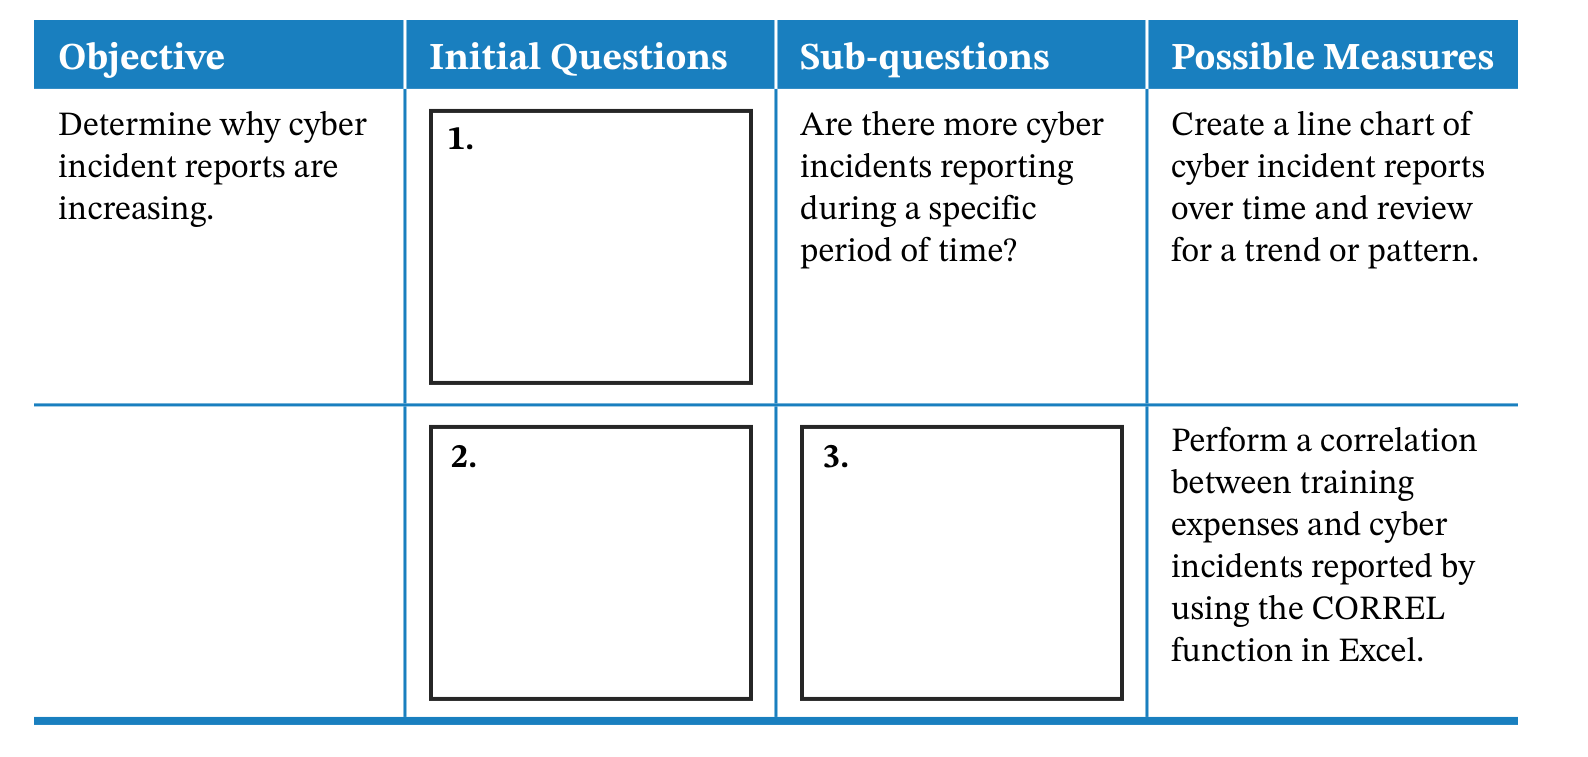
\includegraphics[width=\textwidth,height=0.7\textheight,keepaspectratio]{../textbookForPractice/Figures/Ch_03/EX 3.8_1.png}
            \end{figure}
        \end{column}
    \end{columns}
\end{frame}

\begin{frame}{EX 3.10 \& EX 3.13}
    \begin{columns}
        \begin{column}{0.5\textwidth}
            \begin{figure}[h]
                \centering
                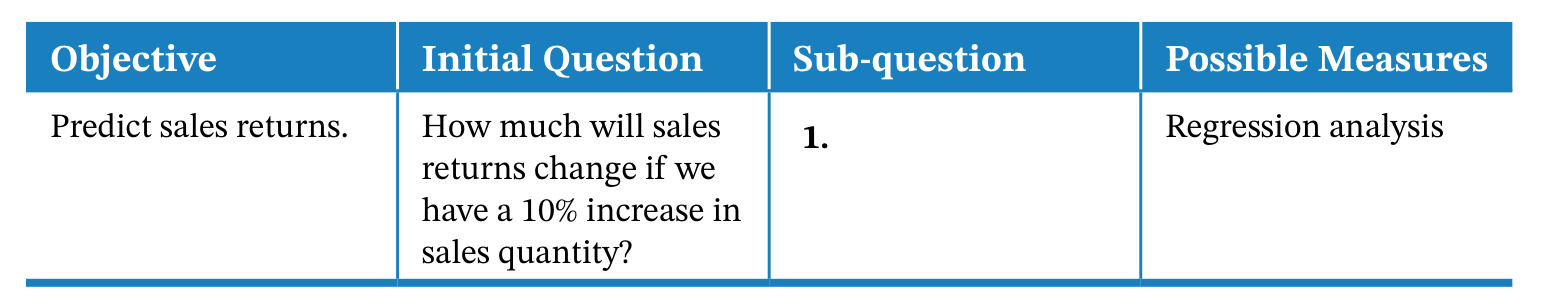
\includegraphics[width=\textwidth,height=0.7\textheight,keepaspectratio]{../textbookForPractice/Figures/Ch_03/EX 3.10.png}
            \end{figure}
        \end{column}
        \begin{column}{0.5\textwidth}
            \begin{figure}[h]
                \centering
                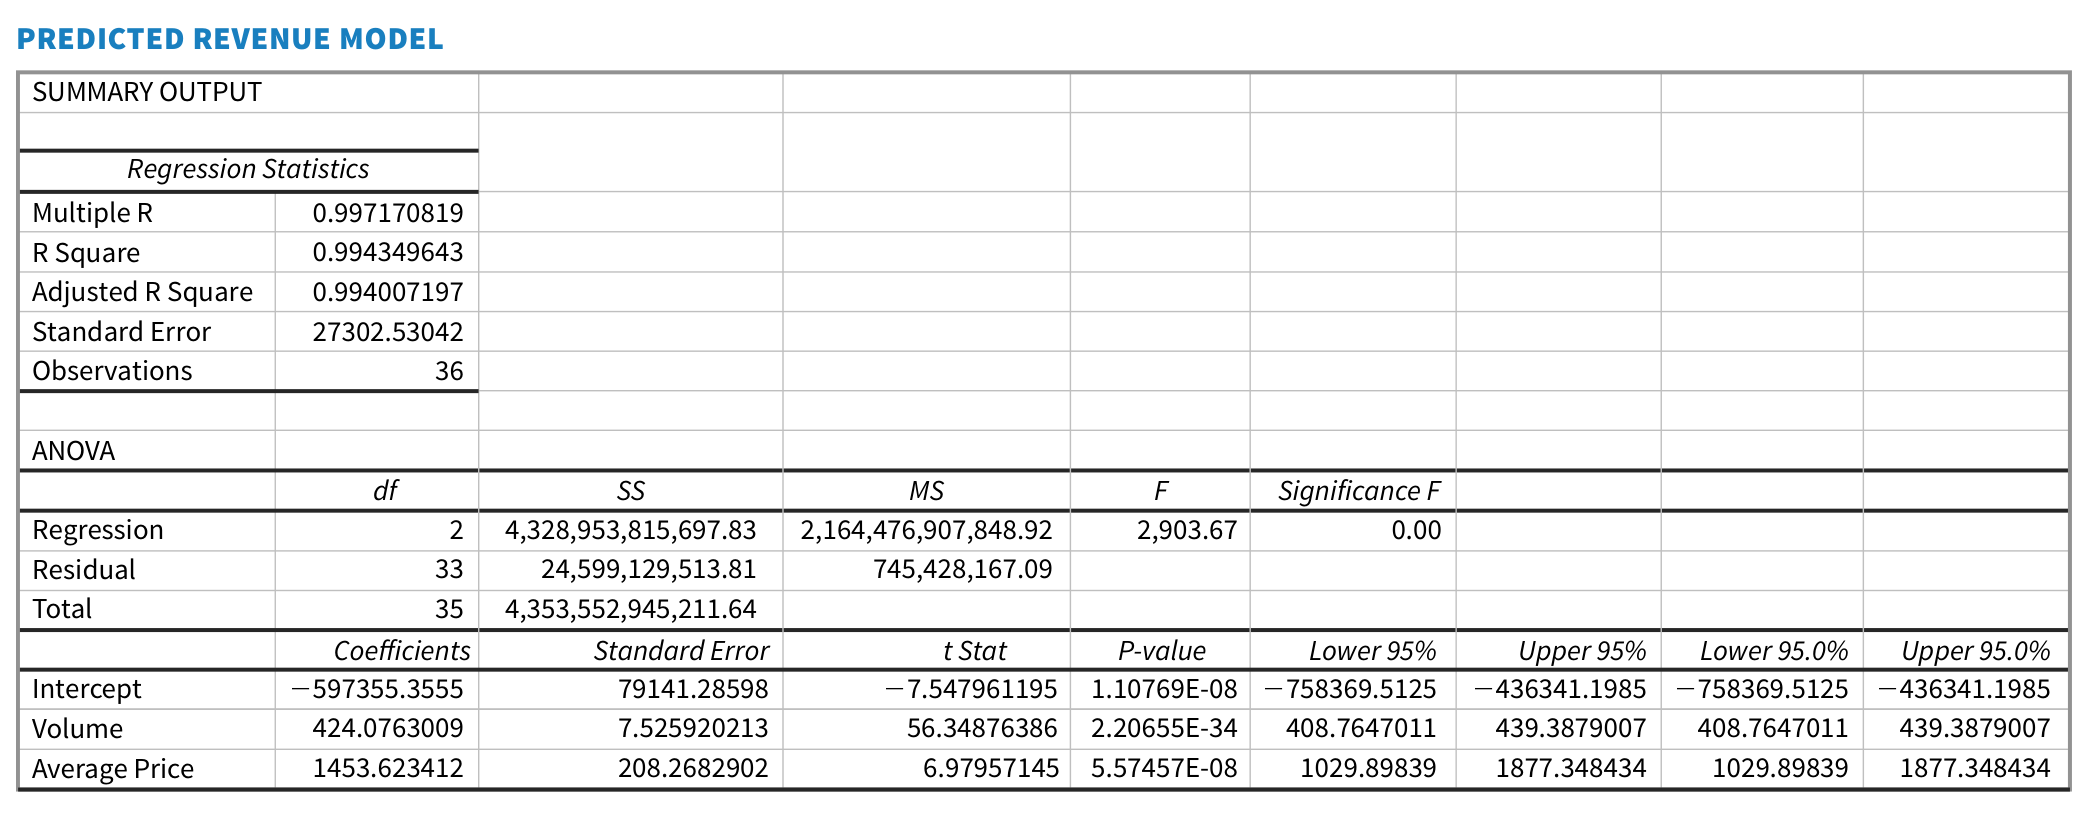
\includegraphics[width=\textwidth,height=0.7\textheight,keepaspectratio]{../textbookForPractice/Figures/Ch_03/EX 3.13.png}
            \end{figure}
        \end{column}
    \end{columns}
\end{frame}

\begin{frame}{EX 3.13\_1 \& EX 3.16}
    \begin{columns}
        \begin{column}{0.5\textwidth}
            \begin{figure}[h]
                \centering
                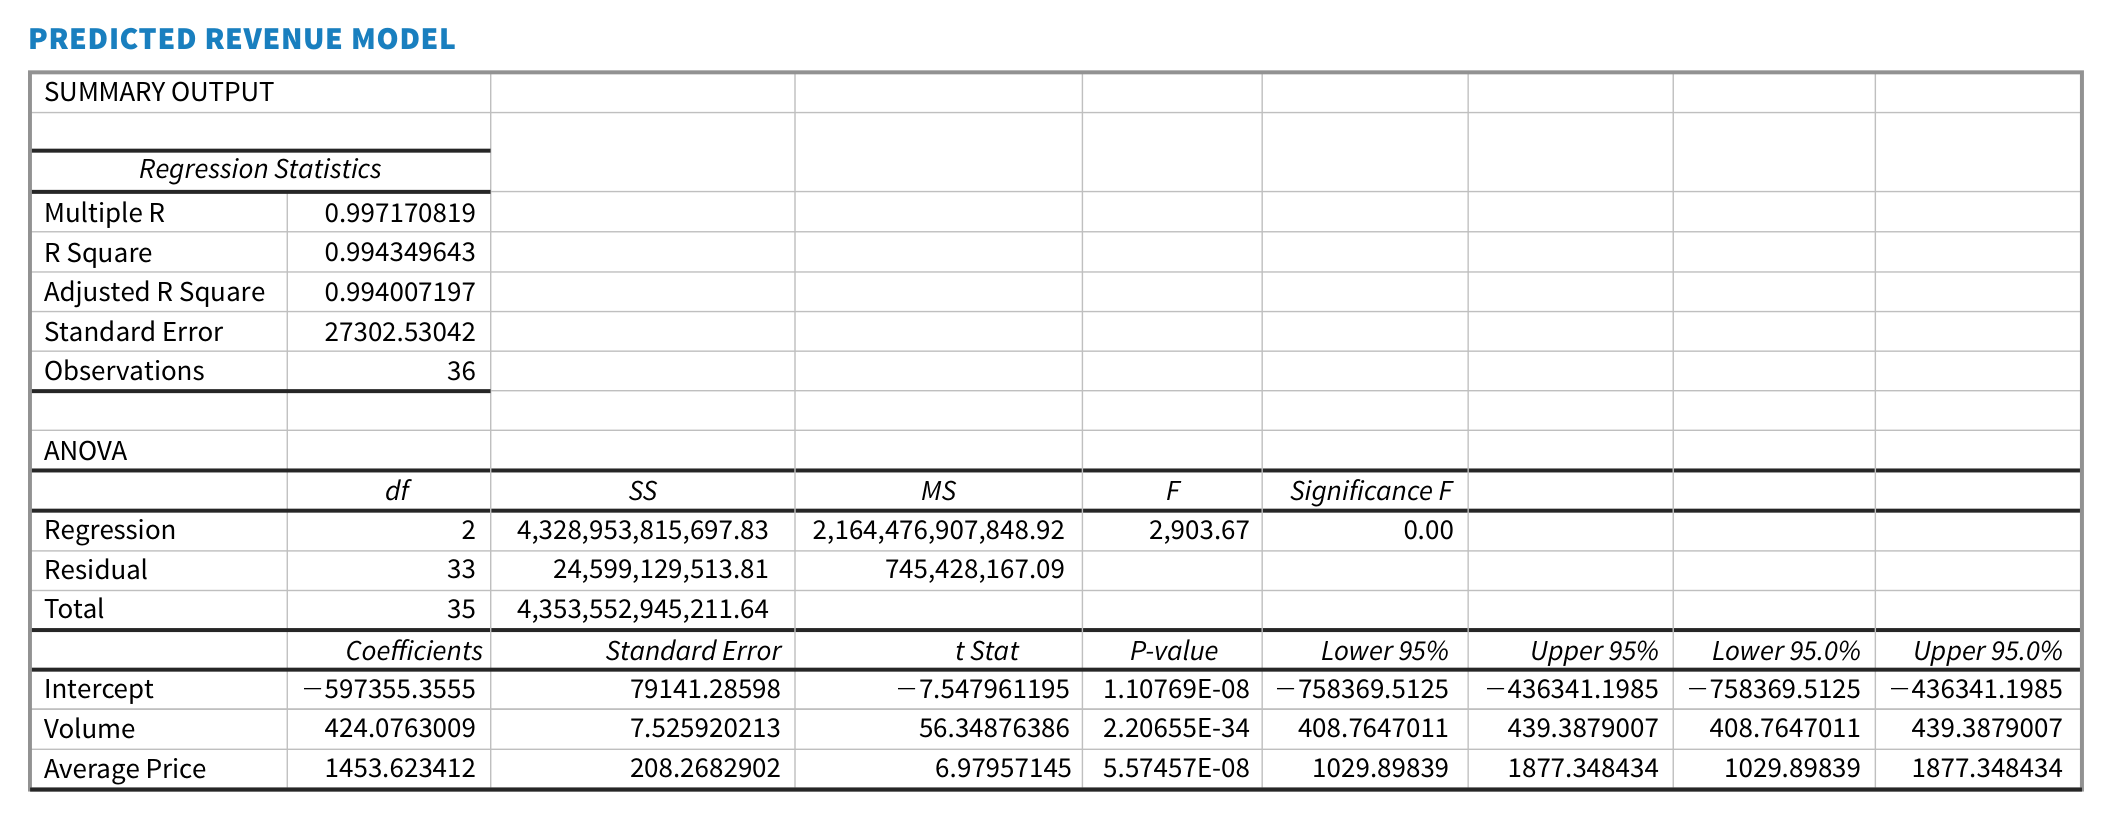
\includegraphics[width=\textwidth,height=0.7\textheight,keepaspectratio]{../textbookForPractice/Figures/Ch_03/EX 3.13_1.png}
            \end{figure}
        \end{column}
        \begin{column}{0.5\textwidth}
            \begin{figure}[h]
                \centering
                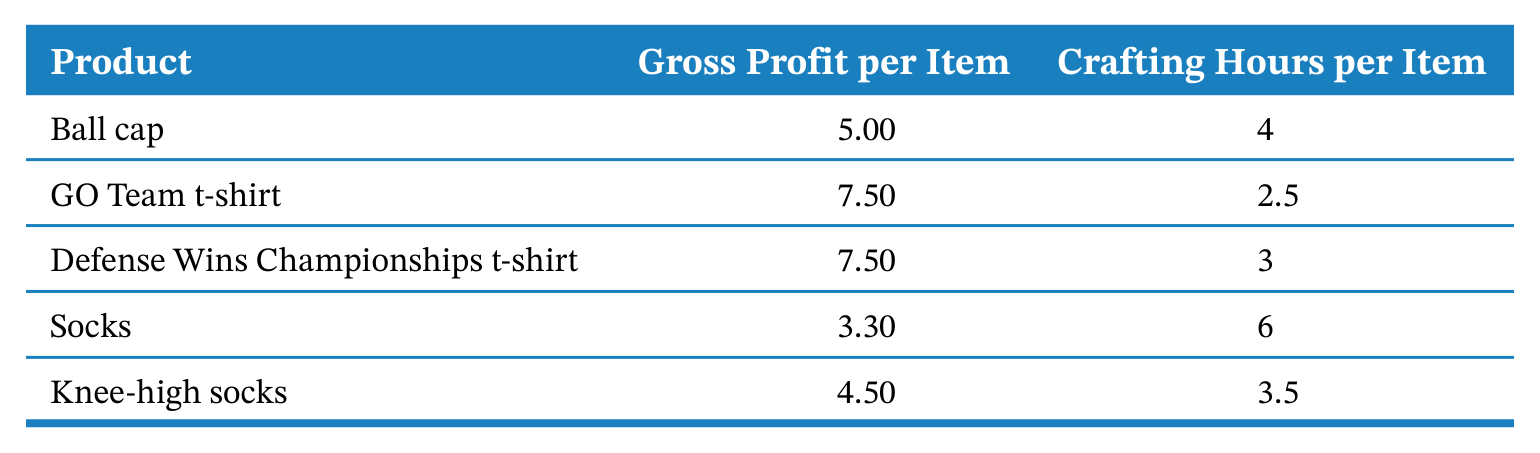
\includegraphics[width=\textwidth,height=0.7\textheight,keepaspectratio]{../textbookForPractice/Figures/Ch_03/EX 3.16.png}
            \end{figure}
        \end{column}
    \end{columns}
\end{frame}

\begin{frame}{EX 3.17}

    \begin{figure}[h]
        \centering
        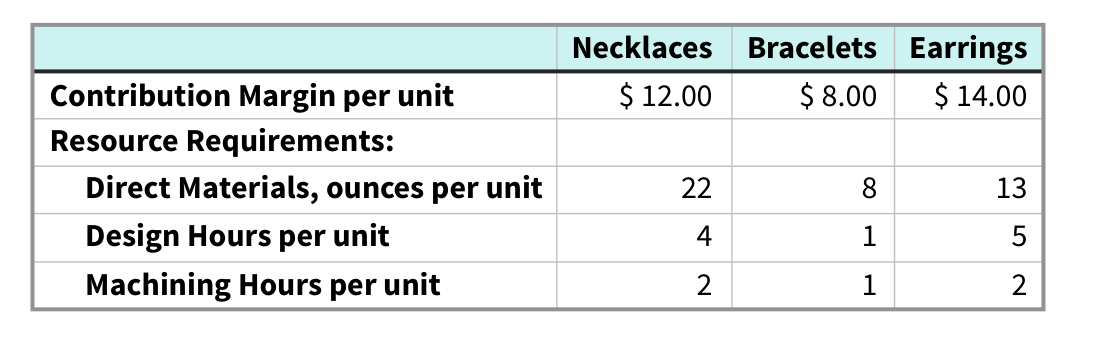
\includegraphics[width=0.95\textwidth,height=0.75\textheight,keepaspectratio]{../textbookForPractice/Figures/Ch_03/EX 3.17.png}
    \end{figure}
\end{frame}

\begin{frame}{Tình huống Ứng dụng (PAC)}
\begin{center}
    \Huge \textbf{Tình huống Ứng dụng Chuyên môn} \\
    \vspace{0.5cm}
    \Large Professional Application Cases (PAC)
\end{center}
\end{frame}

\begin{frame}{PAC 3.1 \& PAC 3.2}
    \begin{columns}
        \begin{column}{0.5\textwidth}
            \begin{figure}[h]
                \centering
                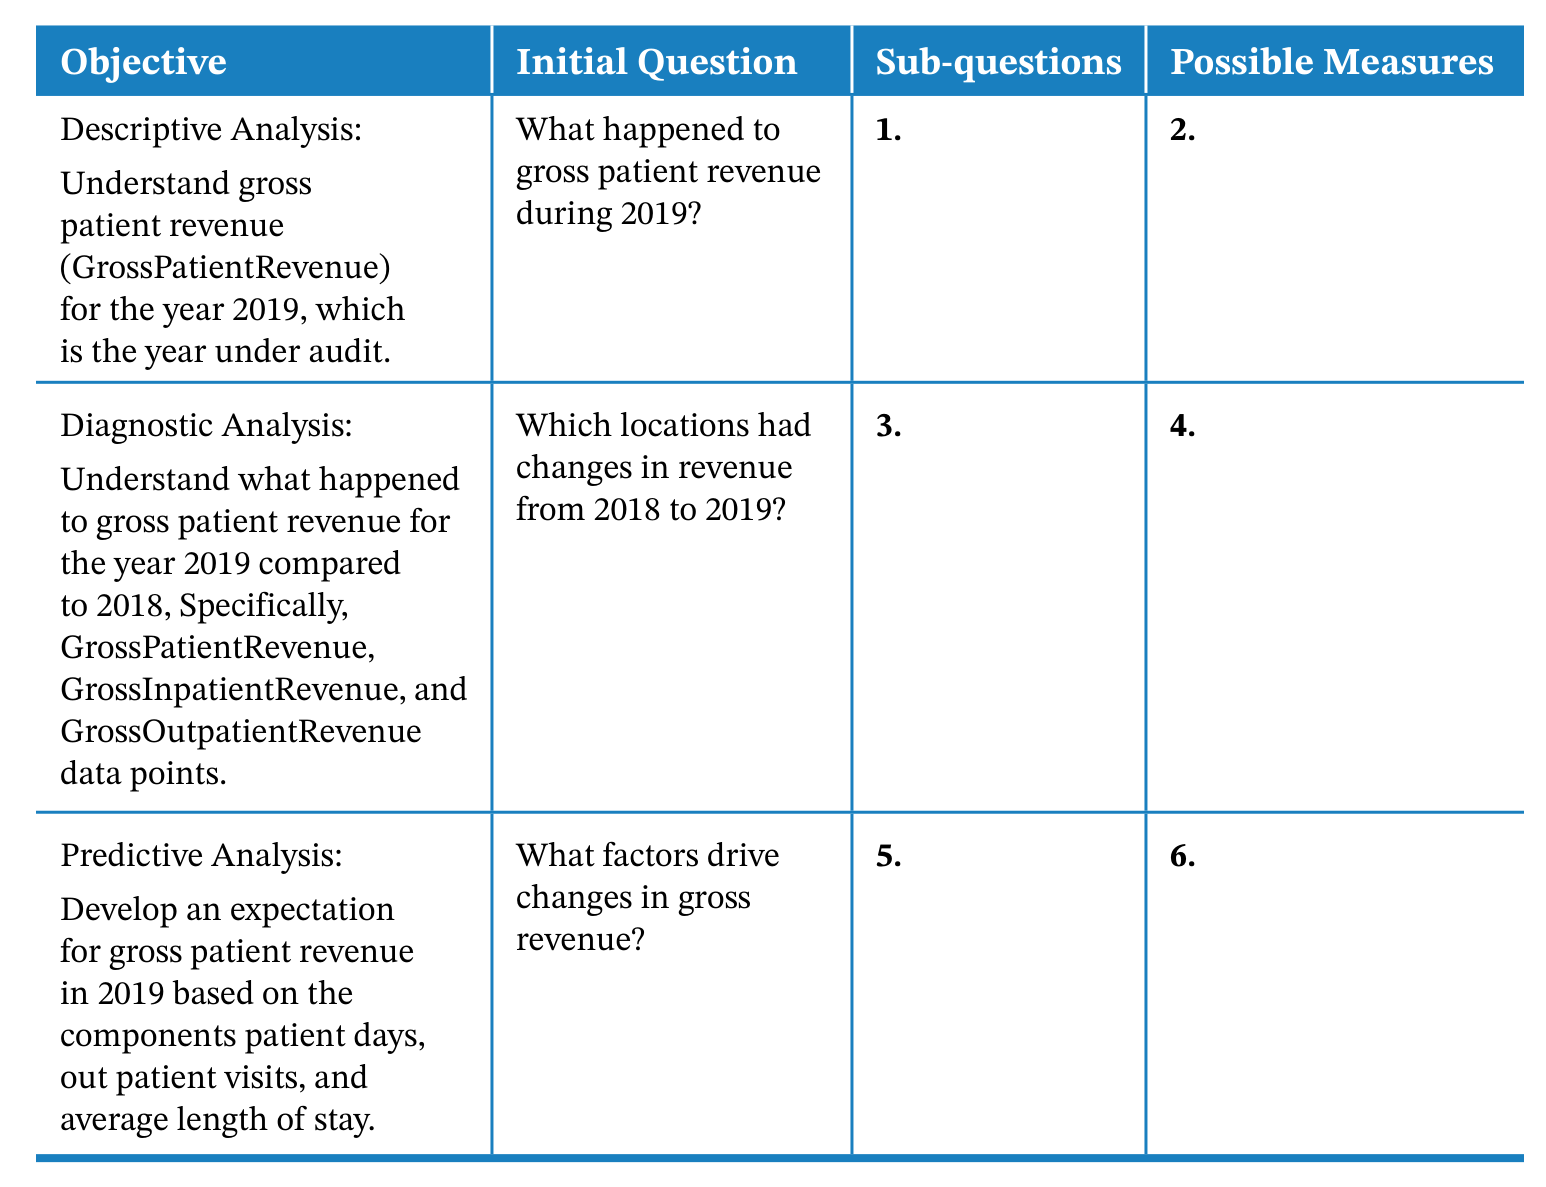
\includegraphics[width=\textwidth,height=0.7\textheight,keepaspectratio]{../textbookForPractice/Figures/Ch_03/PAC 3.1.png}
            \end{figure}
        \end{column}
        \begin{column}{0.5\textwidth}
            \begin{figure}[h]
                \centering
                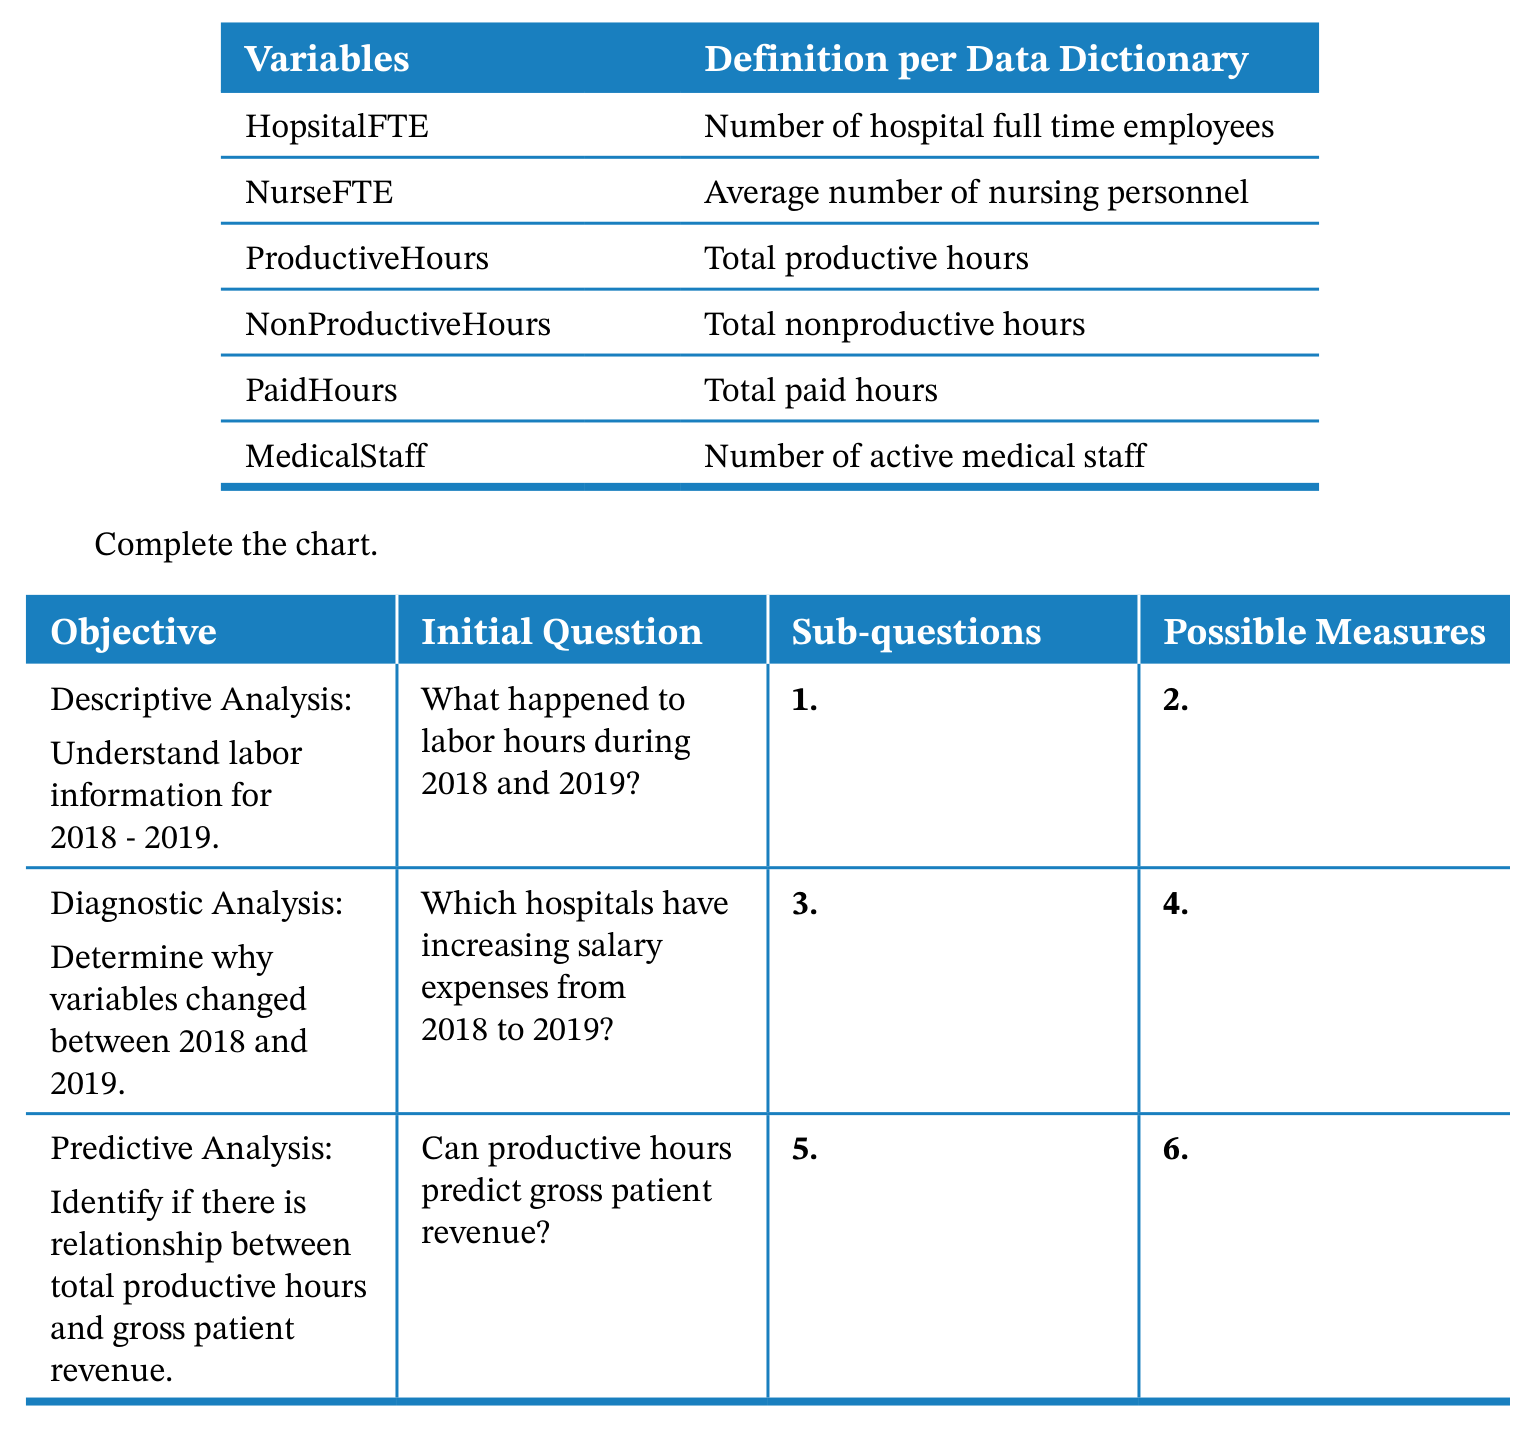
\includegraphics[width=\textwidth,height=0.7\textheight,keepaspectratio]{../textbookForPractice/Figures/Ch_03/PAC 3.2.png}
            \end{figure}
        \end{column}
    \end{columns}
\end{frame}

\begin{frame}{PAC 3.3 \& PAC 3.4}
    \begin{columns}
        \begin{column}{0.5\textwidth}
            \begin{figure}[h]
                \centering
                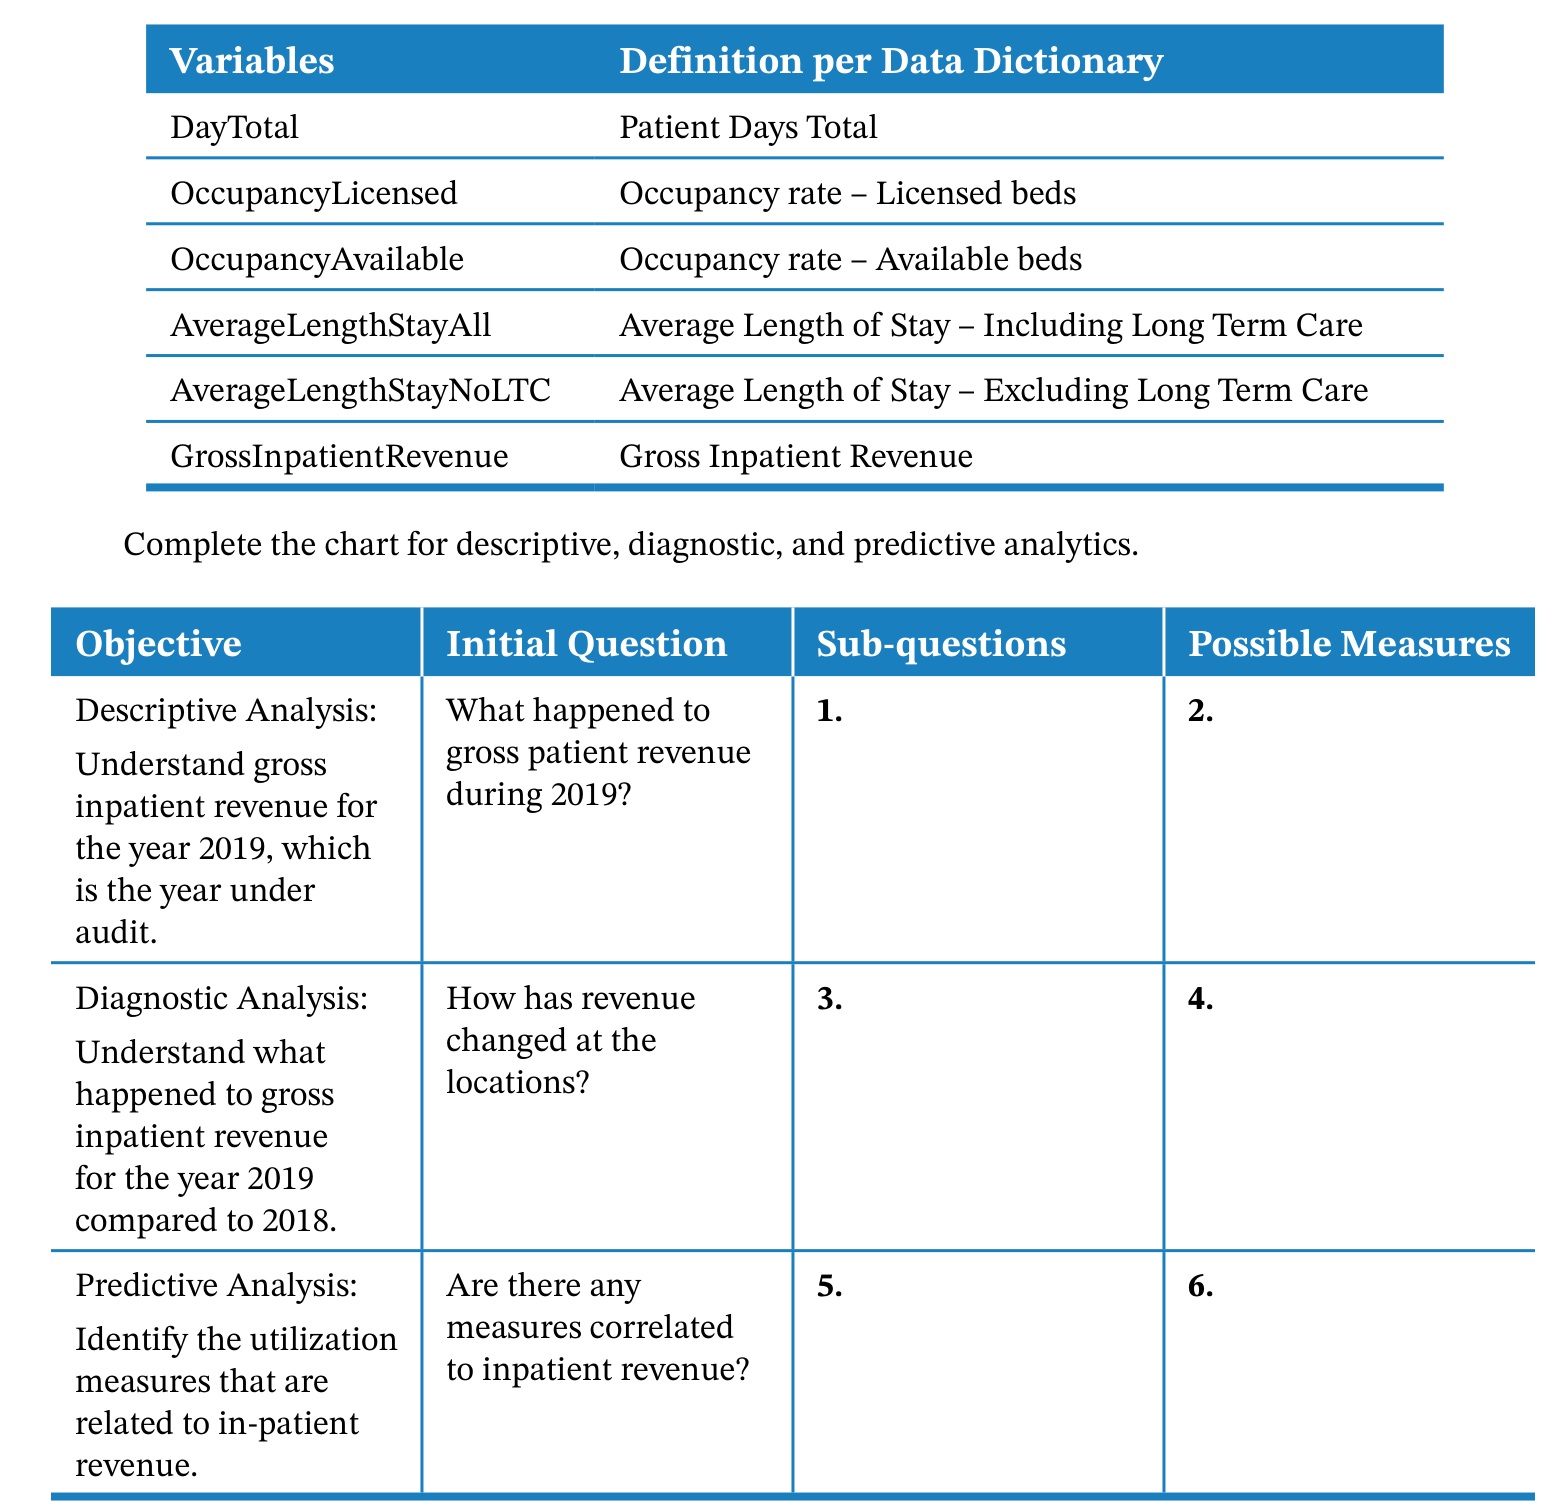
\includegraphics[width=\textwidth,height=0.7\textheight,keepaspectratio]{../textbookForPractice/Figures/Ch_03/PAC 3.3.png}
            \end{figure}
        \end{column}
        \begin{column}{0.5\textwidth}
            \begin{figure}[h]
                \centering
                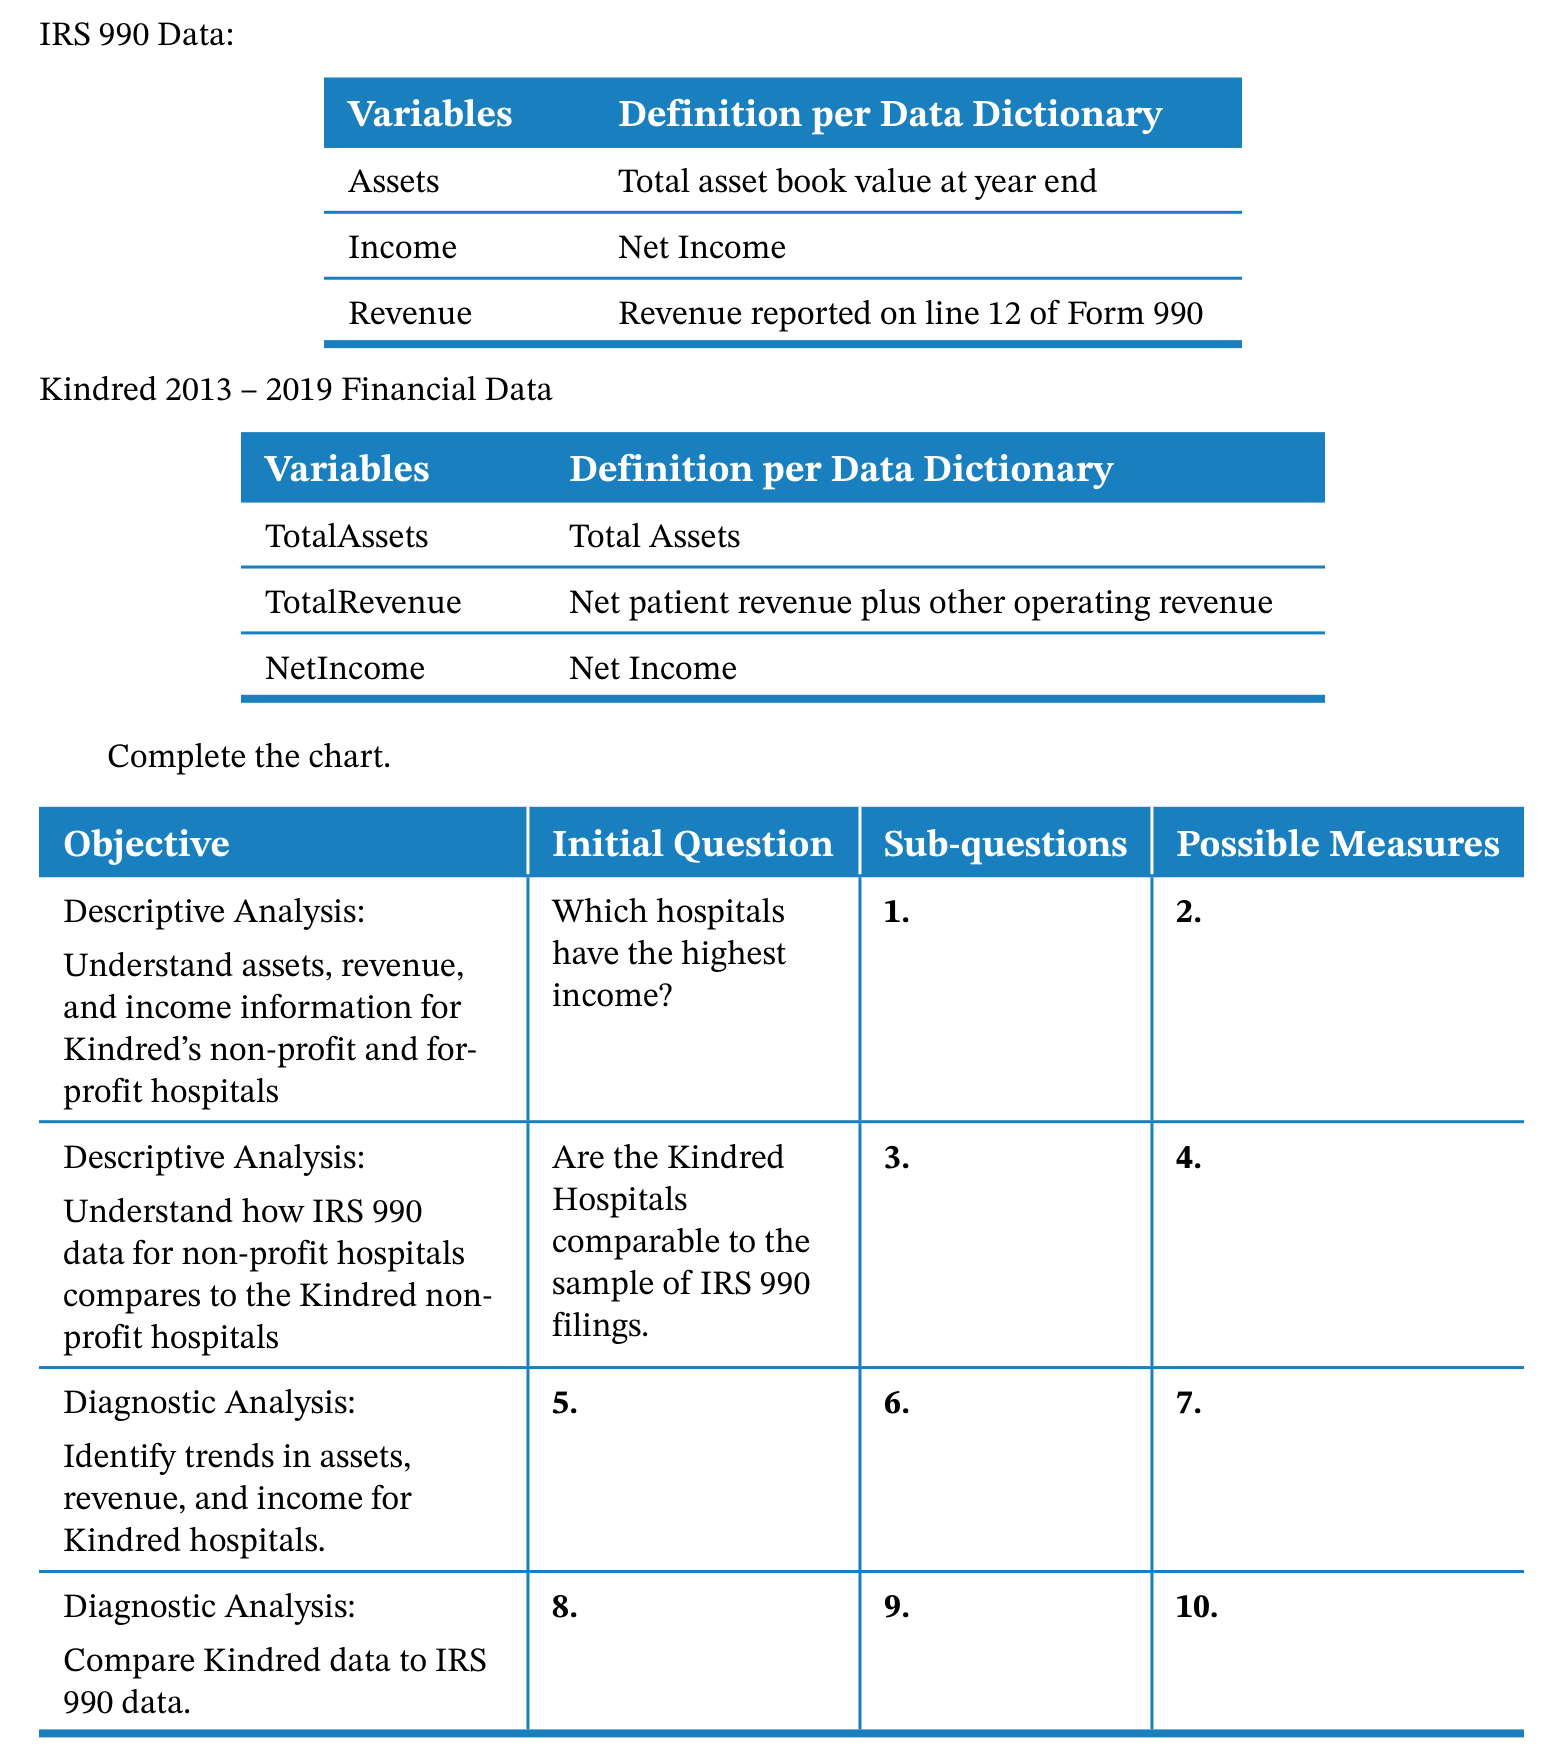
\includegraphics[width=\textwidth,height=0.7\textheight,keepaspectratio]{../textbookForPractice/Figures/Ch_03/PAC 3.4.png}
            \end{figure}
        \end{column}
    \end{columns}
\end{frame}

\begin{frame}{Các Tài liệu \& Tình huống Khác}
\begin{center}
    \Huge \textbf{Tài liệu Bổ sung}
\end{center}
\end{frame}

\begin{frame}{Case 3.13}

    \begin{figure}[h]
        \centering
        
\includegraphics[width=0.95\textwidth,height=0.75\textheight,keepaspectratio]{../textbookForPractice/Figures/Ch_03/Case 3.13.png}
    \end{figure}
\end{frame}

\begin{frame}{Healthcare service company 3.1}

    \begin{figure}[h]
        \centering
        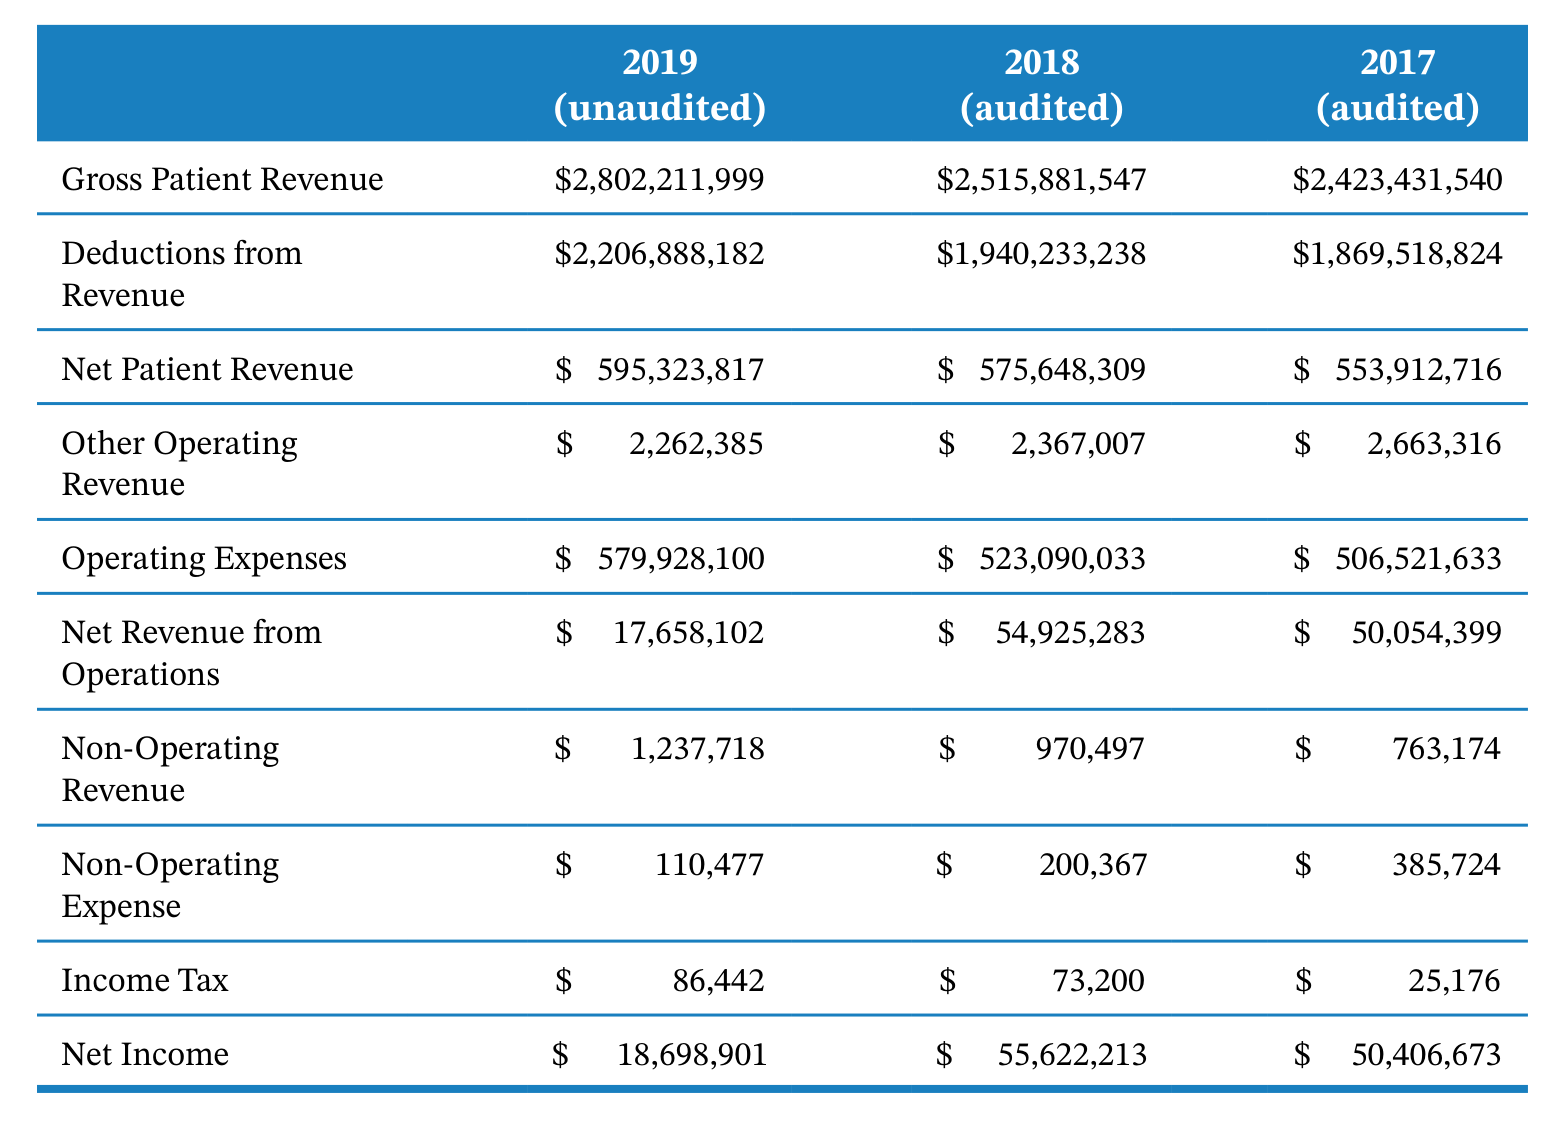
\includegraphics[width=0.95\textwidth,height=0.75\textheight,keepaspectratio]{../textbookForPractice/Figures/Ch_03/Healthcare service company 3.1.png}
    \end{figure}
\end{frame}

\begin{frame}{Info 3.1}

    \begin{figure}[h]
        \centering
        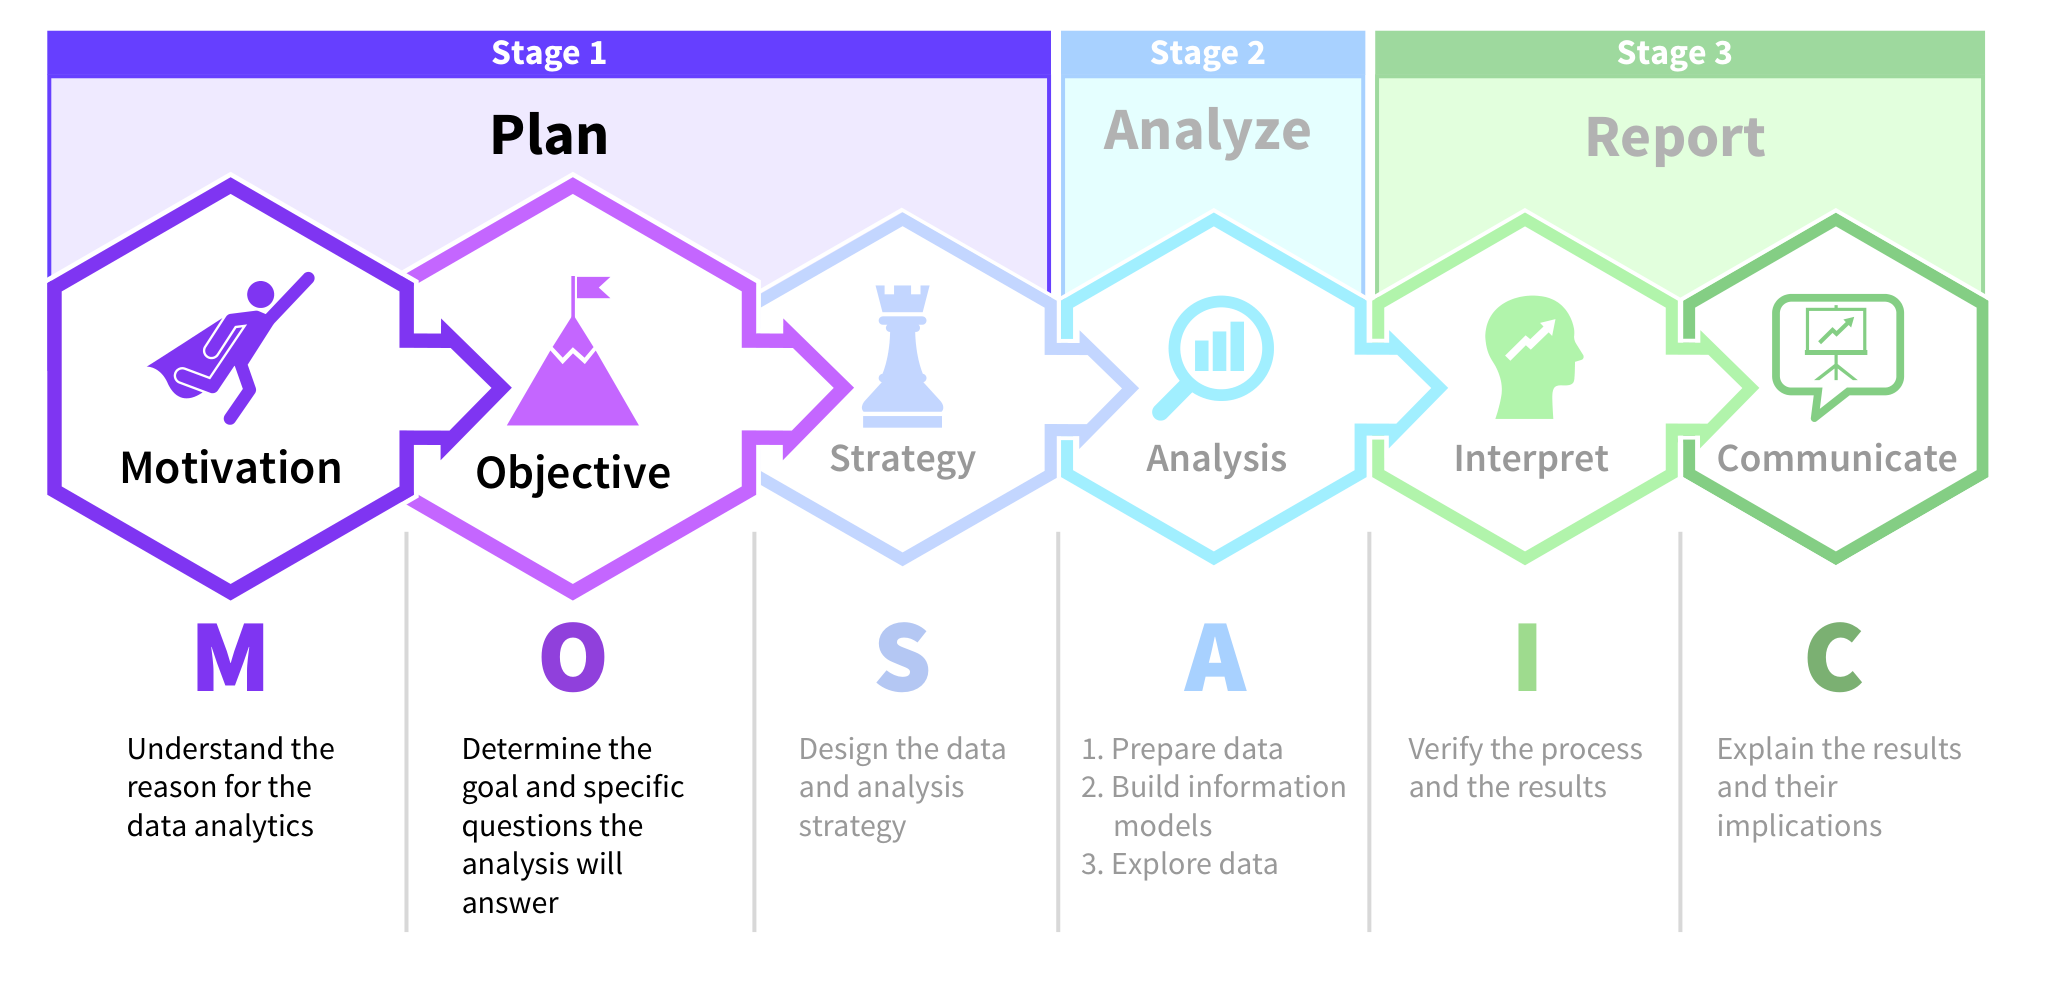
\includegraphics[width=0.95\textwidth,height=0.75\textheight,keepaspectratio]{../textbookForPractice/Figures/Ch_03/Info 3.1.png}
    \end{figure}
\end{frame}

\begin{frame}{Kết thúc}
    \begin{center}
        \Huge \textbf{Hỏi \& Đáp} \\
        \vspace{1cm}
        \Large Cảm ơn các bạn đã lắng nghe!
    \end{center}
\end{frame}

\end{document}
